\documentclass[12pt, twoside]{Thesis} 

\graphicspath{{Pictures/}} 

\usepackage[square, numbers, comma, sort&compress]{natbib} % Use the natbib reference package - read up on this to edit the reference style; if you want text (e.g. Smith et al., 2012) for the in-text references (instead of numbers), remove 'numbers' 
\usepackage{caption}
\usepackage{url}
\usepackage{subcaption}
\usepackage{notoccite,adjustbox}
\usepackage[croatian, british]{babel}
\selectlanguage{british}

\setlength\parindent{24pt}
\hypersetup{urlcolor=blue, colorlinks=true} % Colors hyperlinks in blue - change to black if annoying
\title{\ttitle} % Defines the thesis title - don't touch this
%\usepackage[left=2.5cm,right=2.5cm,top=2.5cm,bottom=2.5cm]{geometry}
\begin{document}

\frontmatter % Use roman page numbering style (i, ii, iii, iv...) for the pre-content pages

\setstretch{1.5} % Line spacing of 1.5

% Define the page headers using the FancyHdr package and set up for one-sided printing
\fancyhead{} % Clears all page headers and footers
%\rfoot{\thepage} % Sets the right side header to show the page number
%\lhead{} % Clears the left side page header
\fancyfoot[LE,RO]{\thepage}
\pagestyle{fancy} % Finally, use the "fancy" page style to implement the FancyHdr headers

\newcommand{\HRule}{\rule{\linewidth}{0.5mm}} % New command to make the lines in the title page

% PDF meta-data
\hypersetup{pdftitle={\ttitle}}
\hypersetup{pdfsubject=\subjectname}
\hypersetup{pdfauthor=\authornames}
\hypersetup{pdfkeywords=\keywordnames}

%----------------------------------------------------------------------------------------
%	TITLE PAGE
%----------------------------------------------------------------------------------------

%\begin{titlepage}
%\begin{center}
%
%\textsc{\LARGE \univname}\\[1.5cm] % University name
%\textsc{\Large Doctoral Thesis}\\[0.5cm] % Thesis type
%
%\HRule \\[0.4cm] % Horizontal line
%{\huge \bfseries \ttitle}\\[0.4cm] % Thesis title
%\HRule \\[1.5cm] % Horizontal line
% 
%\begin{minipage}{0.4\textwidth}
%\begin{flushleft} \large
%\emph{Author:}\\
%{\authornames} % Author name - remove the \href bracket to remove the link
%\end{flushleft}
%\end{minipage}
%\begin{minipage}{0.4\textwidth}
%\begin{flushright} \large
%\emph{Supervisor:} \\
%{\supname} % Supervisor name - remove the \href bracket to remove the link  
%\end{flushright}
%\end{minipage}\\[3cm]
% 
%\large \textit{A thesis submitted in fulfilment of the requirements\\ for the degree of \degreename}\\[0.3cm] % University requirement text
%\textit{in the}\\[0.4cm]
%\groupname\\\deptname\\[2cm] % Research group name and department name
% 
%{\large \today}\\[4cm] % Date
%%\includegraphics{Logo} % University/department logo - uncomment to place it
% 
%\vfill
%\end{center}
%
%\end{titlepage}

%----------------------------------------------------------------------------------------
%	DECLARATION PAGE
%	Your institution may give you a different text to place here
%----------------------------------------------------------------------------------------

%\Declaration{
%
%\addtocontents{toc}{\vspace{1em}} % Add a gap in the Contents, for aesthetics
%
%I, \authornames, declare that this thesis titled, '\ttitle' and the work presented in it are my own. I confirm that:
%
%\begin{itemize} 
%\item[\tiny{$\blacksquare$}] This work was done wholly or mainly while in candidature for a research degree at this University.
%\item[\tiny{$\blacksquare$}] Where any part of this thesis has previously been submitted for a degree or any other qualification at this University or any other institution, this has been clearly stated.
%\item[\tiny{$\blacksquare$}] Where I have consulted the published work of others, this is always clearly attributed.
%\item[\tiny{$\blacksquare$}] Where I have quoted from the work of others, the source is always given. With the exception of such quotations, this thesis is entirely my own work.
%\item[\tiny{$\blacksquare$}] I have acknowledged all main sources of help.
%\item[\tiny{$\blacksquare$}] Where the thesis is based on work done by myself jointly with others, I have made clear exactly what was done by others and what I have contributed myself.\\
%\end{itemize}
% 
%Signed:\\
%\rule[1em]{25em}{0.5pt} % This prints a line for the signature
% 
%Date:\\
%\rule[1em]{25em}{0.5pt} % This prints a line to write the date
%}
%
%\clearpage % Start a new page
\begin{titlepage}
  \fontsize{16pt}{20pt}\selectfont
  \fontfamily{phv}\fontseries{mc}\selectfont
  %\newgeometry{left=3cm,right=3cm,top=3cm,bottom=2.5cm}
  \setlength{\intextsep}{0pt plus 0pt minus 0pt}

  \begin{center}
    \begin{figure}[ht!]
      \begin{center}
        
\includegraphics[height=4.1184cm, width=5.94cm]{logo_unizg_eng}
      \end{center}
    \end{figure}
    \vspace{0cm}
    {FACULTY OF SCIENCE} \\
    \vspace{3cm}
    Jelena Luetić \\
    \vspace{2cm}
    {\fontsize{22pt}{22pt}\selectfont\textbf{Measurement of the cross section for associated production of a W boson and two b quarks with the CMS detector at the Large Hadron Collider}} \\
    \vspace{2cm}  
    DOCTORAL THESIS \\    
    \vfill{Zagreb, 2015.}
  \end{center}
  %\restoregeometry
\end{titlepage}
%%%%%%%%%%%%%% Prva UNUTARNJA STRANICA / SECOND INNER PAGE %%%%%%%%%%%%%%%
\begin{titlepage}
  \fontsize{16pt}{20pt}\selectfont
  \fontfamily{phv}\fontseries{mc}\selectfont
  %\newgeometry{left=3cm,right=3cm,top=3cm,bottom=2.5cm}
  \setlength{\intextsep}{0pt plus 0pt minus 0pt}

  \begin{center}
    \begin{figure}[ht!]
      \begin{center}
        
\includegraphics[height=4.1184cm, width=5.94cm]{logo_unizg_eng}
      \end{center}
    \end{figure}		
    \vspace{0cm}
    {\fontsize{16pt}{16pt}{FACULTY OF SCIENCE}} \\
    \vspace{1.8cm}
    Jelena Luetić \\
    \vspace{1.8cm}
    {\fontsize{22pt}{22pt}\selectfont\textbf{Measurement of the cross section for associated production of a W boson and two b quarks with the CMS detector at the Large Hadron Collider}} \\
    \vspace{2cm}   
    DOCTORAL THESIS \\  
    \vspace{2cm}   % adjust this spacing if necessary
    Supervisor:\\Professor Vuko Brigljević, PhD \\
    \vfill{Zagreb, 2015}
  \end{center}
  %\restoregeometry
\end{titlepage}
%%%%%%%%%%%%%%% Druga UNUTARNJA STRANICA / FIRST INNER PAGE %%%%%%%%%%%%%%%%
\begin{titlepage}
  \fontsize{16pt}{20pt}\selectfont
  \fontfamily{phv}\fontseries{mc}\selectfont
  %\newgeometry{left=3cm,right=3cm,top=3cm,bottom=2.5cm}
  \setlength{\intextsep}{0pt plus 0pt minus 0pt}

  \begin{center}
    \begin{figure}[ht!]
      \begin{center}
        
\includegraphics[height=4.1184cm, width=5.94cm]{logo_unizg2}
      \end{center}
    \end{figure}		
    \vspace{0cm}
    {PRIRODOSLOVNO MATEMATIČKI FAKULTET} \\
    \vspace{1.8cm}
    Jelena Luetić \\
    \vspace{1.8cm}
    {\fontsize{22pt}{22pt}\selectfont\textbf{Mjerenje udarnog presjeka zajedničke tvorbe W bozona i para b kvarkova detektorom CMS na Velikom hadronskom sudarivaču}} \\
    \vspace{2cm}    
    DOKTORSKI RAD \\
    \vspace{2cm}    % adjust this spacing if necessary
    Mentor:\\Prof. dr. sc. Vuko Brigljević \\
    \vfill{Zagreb, 2015.}
  \end{center}
  %\restoregeometry
\end{titlepage}


%----------------------------------------------------------------------------------------
%	QUOTATION PAGE
%----------------------------------------------------------------------------------------

\pagestyle{empty} % No headers or footers for the following pages

\null\vfill % Add some space to move the quote down the page a bit

%\textit{``Thanks to my solid academic training, today I can write hundreds of words on virtually any topic without possessing a shred of information, which is how I got a good job in journalism."}
\textit{``Each time new experiments are observed to agree with the predictions, the theory survives and our confidence in it is increased; but if ever a new observation is found to disagree, we have to abandon or modify the theory. \\ At least that is what it is supposed to happen, but you can always question the competence of the person who carried out the observation."}

\begin{flushright}
Stephan Hawking
\end{flushright}

\vfill\vfill\vfill\vfill\vfill\vfill\null % Add some space at the bottom to position the quote just right

\clearpage % Start a new page

%----------------------------------------------------------------------------------------
%	ABSTRACT PAGE
%----------------------------------------------------------------------------------------

\addtotoc{Abstract} % Add the "Abstract" page entry to the Contents

\abstract{\addtocontents{toc}{\vspace{1em}} % Add a gap in the Contents, for aesthetics
   
\par The goal of this thesis is a measurement of the cross section of the $pp\rightarrow W+bb+X$ process using the data collected during 2012 at $\sqrt{s} = 8$ TeV. The data is provided by the Large Hadron Collider (LHC) accelerator at CERN, Geneva and collected by the Compact Muon Solenoid (CMS). The production of a W boson in association with a pair of b quarks (Wbb) in proton collisions has been the topic of many theoretical calculations and simulations. It is however still not well described due to divergences which arise in theoretical calculations, in cases where b quarks are collinear or there is a low energy massless particle irradiated. A precise measurement of Wbb production will allow to further constrain theoretical predictions in the framework of perturbative quantum chromodynamics (pQCD). On the other hand, Wbb is a background in the measurements of different standard model processes as well as in several searches for physics beyond standard model. 
\par The presence of a W boson is identified through the detection of an energetic, isolated lepton (muon or electron) and a significant amount of missing energy, which indicates the presence of a neutrino. Jets in the detector are identified as collimated sprays of particles. Selected jets are required to be tagged as jets originating from b quarks. 
\par The cross section measurement was performed in the fiducial region defined by a presence of a lepton and exactly two 2 b-tagged jets. The result is quoted separately in the muon and electron channel. The measured values in the two channels are compatible, as predicted by the standard model. The theoretical cross section was derived using MCFM. The measured values are around one standard deviation higher than the predicted theoretical values. 
The uncertainty on the measured values is dominated by the systematic effects. The largest uncertainties are associated with the b tagging procedure, jet energy scale and jet energy resolution. Reducing these uncertainties in the future, would allow for more sensitive test of perturbative QCD calculation at next-to-leading order.
}

\textbf{Keywords:} LHC, CMS, Standard model, Wbb, cross section

\clearpage % Start a new page

%----------------------------------------------------------------------------------------
%	ACKNOWLEDGEMENTS
%----------------------------------------------------------------------------------------

\setstretch{1.5} % Reset the line-spacing to 1.3 for body text (if it has changed)

\acknowledgements{\addtocontents{toc}{\vspace{1em}} % Add a gap in the Contents, for aesthetics

I would like to thank all the people who helped make this thesis see the light of day. Thanks to the colegues from University of Wisconsin-Madison, University of Trieste and CERN, specially to Tom , Andrea and others for all their effort and help during past year. Big thanks to Michele for his guidance, patience and precious comments.
\par I would like to thank to all the CMS group from Ruđer Bošković Institute. Thanks to Lucija for being a good friend and listener when I needed one. Thanks to Tanja for all her help and hard work and fruitful discussions, without you this would be nearly half as fun. Thanks to Srećko, Senka, Darko, Saša and Benjamin for all the help and interesting discussions over the past few years. 
Special thanks to my supervisor Vuko Brigljević for helping me and believing in me over the past few years. 
\par Thanks to the Pixel group, specially to Danek, Viktor, Gino, Janos, Urs, Annapaola and others for giving me a chance to work on something new and exciting. 
\par Special thanks to my family for all their support and patience. Without you none of this would be possible.
\par Goran, thank you for being there for me and making me happy. 
}
\clearpage % Start a new page

%----------------------------------------------------------------------------------------
%	LIST OF CONTENTS/FIGURES/TABLES PAGES
%----------------------------------------------------------------------------------------

\pagestyle{fancy} % The page style headers have been "empty" all this time, now use the "fancy" headers as defined before to bring them back

\fancyhead[LE,RO]{\emph{Contents}} % Set the left side page header to "Contents"
\tableofcontents % Write out the Table of Contents

\fancyhead[LE,RO]{\emph{List of Figures}} % Set the left side page header to "List of Figures"
\listoffigures % Write out the List of Figures

\fancyhead[LE,RO]{\emph{List of Tables}} % Set the left side page header to "List of Tables"
\listoftables % Write out the List of Tables

%----------------------------------------------------------------------------------------
%	ABBREVIATIONS
%----------------------------------------------------------------------------------------

\clearpage % Start a new page

\setstretch{1.5} % Set the line spacing to 1.5, this makes the following tables easier to read

\fancyhead[LE,RO]{\emph{Abbreviations}} % Set the left side page header to "Abbreviations"
\listofsymbols{ll} % Include a list of Abbreviations (a table of two columns)
{
\textbf{SM} & Standard Model \\
\textbf{CERN} & European Organization for Nuclear Research \\
\textbf{LHC} & Large Hadron Collider \\
\textbf{CMS} & Compact Muon Solenoid \\
\textbf{CP} & Charge-parity \\
\textbf{CKM} & Cabibbo-Kobayashi-Maskawa matrix \\
\textbf{QCD} & Quantum chromodynamics \\
\textbf{LO} & Leading order \\
\textbf{NLO} & Next-to-leading order \\ 
\textbf{DPS} & Double Parton Scattering \\
\textbf{ECAL} & Electromagnetic Calorimeter \\
\textbf{HCAL} & Hadronic Calorimeter \\
\textbf{CSC} & Cathode Strip Chamber \\ 
\textbf{RPC} & Resistive Plate Chambers \\  
\textbf{DT} & Drift Tubes \\
\textbf{L1} & Level 1 Trigger \\
\textbf{HLT} & High Level Trigger \\
\textbf{PF} & Particle Flow \\
\textbf{GSF} & Gaussian Sum Filter \\
\textbf{CSV} & Combined Secondary Vertex \\
\\
}

%----------------------------------------------------------------------------------------
%	PHYSICAL CONSTANTS/OTHER DEFINITIONS
%----------------------------------------------------------------------------------------
%
%\clearpage % Start a new page
%
%\lhead{\emph{Physical Constants}} % Set the left side page header to "Physical Constants"
%
%\listofconstants{lrcl} % Include a list of Physical Constants (a four column table)
%{
%Speed of Light & $c$ & $=$ & $2.997\ 924\ 58\times10^{8}\ \mbox{ms}^{-\mbox{s}}$ (exact)\\
%% Constant Name & Symbol & = & Constant Value (with units) \\
%}

%----------------------------------------------------------------------------------------
%	SYMBOLS
%----------------------------------------------------------------------------------------

%\clearpage % Start a new page
%
%\lhead{\emph{Symbols}} % Set the left side page header to "Symbols"
%
%\listofnomenclature{lll} % Include a list of Symbols (a three column table)
%{
%$a$ & distance & m \\
%$P$ & power & W (Js$^{-1}$) \\
%% Symbol & Name & Unit \\\fancyhead[LE,RO]\fancyhead[LE,RO]
%
%& & \\ % Gap to separate the Roman symbols from the Greek
%
%$\omega$ & angular frequency & rads$^{-1}$ \\
%% Symbol & Name & Unit \\
%}

%----------------------------------------------------------------------------------------
%	DEDICATION
%----------------------------------------------------------------------------------------

%\setstretch{1.5} % Return the line spacing back to 1.3

%\pagestyle{empty} % Page style needs to be empty for this page

%\dedicatory{For my Gogi.} % Dedication text

%\addtocontents{toc}{\vspace{2em}} % Add a gap in the Contents, for aesthetics

%----------------------------------------------------------------------------------------
%	THESIS CONTENT - CHAPTERS
%----------------------------------------------------------------------------------------

\mainmatter % Begin numeric (1,2,3...) page numbering

\pagestyle{fancy} % Return the page headers back to the "fancy" style

% Include the chapters of the thesis as separate files from the Chapters folder
% Uncomment the lines as you write the chapters

% Chapter 1

\chapter{Introduction} % Main chapter title

\label{Chapter1} % For referencing the chapter elsewhere, use \ref{Chapter1} 

\lhead{Chapter 1. \emph{Introduction}} % This is for the header on each page - perhaps a shortened title

% Filozofija
The standard model of particle physics tries to give an answer to the questions what is the matter made of and how does it interact. The predictions of the standard model have been thoroughly tested many times and various precision measurements were performed at different experiments. Nevertheless every time the standard model predictions were confirmed. The only missing link, the long sought Higgs boson, was found in 2012, with its properties measured in the following years thus completing the picture of elementary particles. However, standard model still leaves some unexplained phenomena, e.g. neutrino oscillations, matter-antimatter asymmetry, the existence of dark matter and dark energy, giving rise to the physics beyond standard model. The sensitivity of such processes in the high energy physics experiments strongly depends on the precise measurements of known processes. In such measurements, poorly known yields and kinematics of the known processes would lead to high uncertainties, and thus reducing the sensitivity of the experiment. 
% Zasto b kvark - QCD
\par The production of a W boson in association with a pair of b quarks (Wbb) has
been the topic of many theoretical studies and simulations. It is however still not well described due to collinear and infrared divergences. Several theoretical
approaches, implemented in different simulation packages, have been used to describe the Wbb production mechanism. A precise measurement of Wbb production will allow to
further constrain theoretical predictions in the framework of perturbative quantum chromodynamics (pQCD) and to test the validity of different theoretical models used in simulations. On the other hand, Wbb is a background to different standard model processes as well as beyond standard model searches. It is one of the main backgrounds to top quark  and Higgs boson measurements, in particular, events in which Higgs boson is produced in association with a W boson and decays to a pair of b quarks.
% Sto je pokazano
\par This thesis is focused on the measurement of the cross section of $pp\rightarrow W+bb+X$ process using the data collected during 2012 at $\sqrt{s} = 8$ TeV. W boson is decaying either to an electron or muon, and a corresponding neutrino. The presence of a W boson is identified through the detection of an energetic, isolated lepton, i.e. lepton without any additional activity in some predefined cone around it, and a significant amount of missing energy, which indicates the presence of a neutrino. Jets in the detector are identified as a collimated spray of particles. Selected jets are required to be tagged as jets originating from b quarks. This procedure is called b-tagging and it exploits unique b quark properties to derive a single discriminator value to distinguish between b jets and jets from lighter quarks, or gluons. 
% Organizacija teze

The thesis is organized as follows. Chapter 2 shows a brief introduction to the standard model, with the emphasis on the discovery and the role of W boson and b quarks within the standard model. An overview of the phenomenology of the proton collisions at hadron colliders is shown. Steps for the theoretical calculation of the $pp\rightarrow W+bb+X$ process are given for both, single parton scattering and double parton scattering production mechanisms. The end of the chapter summarizes all previous measurements of W boson and b quarks in the final state. Chapters 3 and 4 are focused on the description of the LHC and CMS respectively. All CMS subsystems are described and their role is explained. Chapter 5 describes the procedure for reconstruction of various physics objects, including electrons, muons and jets, and estimation of missing energy. Chapter 6 lists all data and Monte Carlo samples used. Criteria for the signal selection is described and all major backgrounds are identified. Chapter 7 describes all steps in the cross section determination, including the fitting procedure used to extract final yields, and the acceptance and efficiency estimation. In the end, the results are presented, together with the comparison to theoretical predictions. Final chapter briefly summarizes the results, and shows the prospects for the future research on this topic.

% Chapter Template

\chapter{Standard Model} % Main chapter title

\label{Chapter2} % Change X to a consecutive number; for referencing this chapter elsewhere, use \ref{ChapterX}

\lhead{Chapter X. \emph{Chapter Title Here}} % Change X to a consecutive number; this is for the header on each page - perhaps a shortened title

%----------------------------------------------------------------------------------------
%	SECTION 1
%----------------------------------------------------------------------------------------

\section{Standard model}

Lorem ipsum dolor sit amet, consectetur adipiscing elit. Aliquam ultricies lacinia euismod. Nam tempus risus in dolor rhoncus in interdum enim tincidunt. Donec vel nunc neque. In condimentum ullamcorper quam non consequat. Fusce sagittis tempor feugiat. Fusce magna erat, molestie eu convallis ut, tempus sed arcu. Quisque molestie, ante a tincidunt ullamcorper, sapien enim dignissim lacus, in semper nibh erat lobortis purus. Integer dapibus ligula ac risus convallis pellentesque.

%-----------------------------------
%	SUBSECTION 1
%-----------------------------------
\subsection{Wbb at hadron collider}

Nunc posuere quam at lectus tristique eu ultrices augue venenatis. Vestibulum ante ipsum primis in faucibus orci luctus et ultrices posuere cubilia Curae; Aliquam erat volutpat. Vivamus sodales tortor eget quam adipiscing in vulputate ante ullamcorper. Sed eros ante, lacinia et sollicitudin et, aliquam sit amet augue. In hac habitasse platea dictumst.

%-----------------------------------
%	SUBSECTION 2
%-----------------------------------

\subsection{Previous measurements}
Morbi rutrum odio eget arcu adipiscing sodales. Aenean et purus a est pulvinar pellentesque. Cras in elit neque, quis varius elit. Phasellus fringilla, nibh eu tempus venenatis, dolor elit posuere quam, quis adipiscing urna leo nec orci. Sed nec nulla auctor odio aliquet consequat. Ut nec nulla in ante ullamcorper aliquam at sed dolor. Phasellus fermentum magna in augue gravida cursus. Cras sed pretium lorem. Pellentesque eget ornare odio. Proin accumsan, massa viverra cursus pharetra, ipsum nisi lobortis velit, a malesuada dolor lorem eu neque.

%----------------------------------------------------------------------------------------
%	SECTION 2
%----------------------------------------------------------------------------------------

\section{Main Section 2}

Sed ullamcorper quam eu nisl interdum at interdum enim egestas. Aliquam placerat justo sed lectus lobortis ut porta nisl porttitor. Vestibulum mi dolor, lacinia molestie gravida at, tempus vitae ligula. Donec eget quam sapien, in viverra eros. Donec pellentesque justo a massa fringilla non vestibulum metus vestibulum. Vestibulum in orci quis felis tempor lacinia. Vivamus ornare ultrices facilisis. Ut hendrerit volutpat vulputate. Morbi condimentum venenatis augue, id porta ipsum vulputate in. Curabitur luctus tempus justo. Vestibulum risus lectus, adipiscing nec condimentum quis, condimentum nec nisl. Aliquam dictum sagittis velit sed iaculis. Morbi tristique augue sit amet nulla pulvinar id facilisis ligula mollis. Nam elit libero, tincidunt ut aliquam at, molestie in quam. Aenean rhoncus vehicula hendrerit. 
% Chapter Template

\chapter{Large Hadron Collider} % Main chapter title

\label{Chapter3} % Change X to a consecutive number; for referencing this chapter elsewhere, use \ref{ChapterX}

\lhead{Chapter 3. \emph{Large Hadron Collider}} % Change X to a consecutive number; this is for the header on each page - perhaps a shortened title

CERN is the largest particle physics laboratory in the world, located near the city of Genava, on the French-Swiss border. It was founded in 1953 by 12 countries and today it has 21 member states. It's main function is to provide particle accelerators and infrastructure for high energy physics experiments. Current accelerator complex is a chain of smaller accelerators with increasingly higher energies of which the largest one is Large Hadron Collider (LHC) (Figure \ref{LHC}). Protons accelerated in the chain are obtained by taking hydrogen atoms and stripping them of the orbiting electrons. Protons are then accelerated by a small linear accelerator Linac2 to 50 MeV and injected to PS Booster. After reaching 1.4 GeV, protons are injected to Proton Synchrotron and accelerated to 25 GeV. Next accelerators in chain are Super Proton Synchrotron (SPS) with energy of 450 GeV, and Large Hadron collider with beam energy of 7 TeV. 
Some of the major physics results at CERN include the discovery of neutral currents, discovery of W and Z bosons, creation of antihydrogen atom and direct observation of CP violation among others. 
In this chapter, we will briefly go through the motivation for the LHC design, building blocks of the LHC will be presented together with the accelerator performance during the past few years.   
\begin{figure}[htbp]
	\centering
		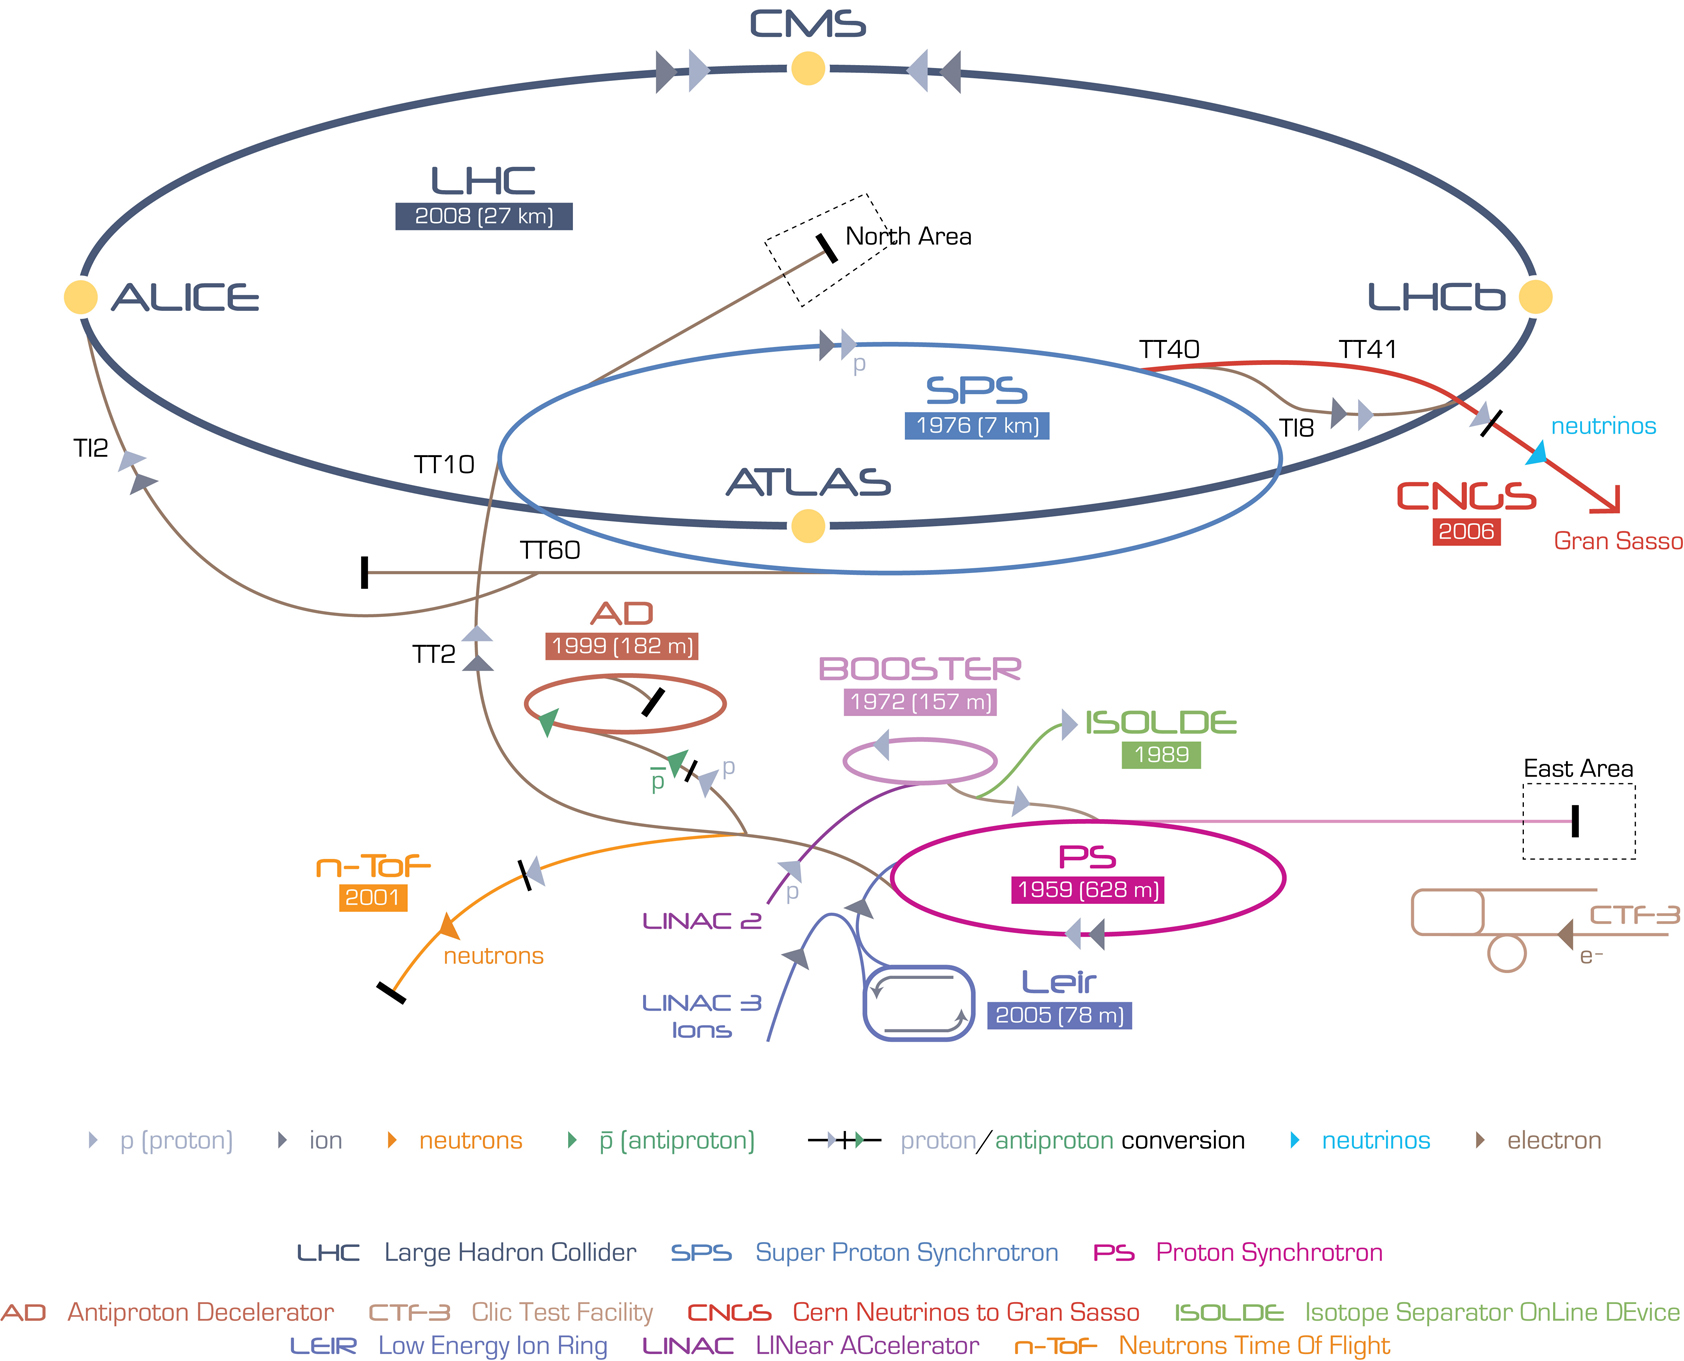
\includegraphics[width=0.8\textwidth]{Figures/LHC.jpg}
		%\rule{35em}{0.5pt}
	\caption[Schematics of Large Hadron Collider]{Schematics of Large Hadron Collider}
	\label{fig:LHC}
\end{figure}
%----------------------------------------------------------------------------------------
%	SECTION 1
%----------------------------------------------------------------------------------------

\section{Design of the Large Hadron Collider}

The Standard model of elementary particles describes nicely all known particles and interactions, however there are still some unanswered questions. One of the major question was the existence of Higgs boson which was solved in the past few years with the discovery of a new particle at 125 GeV. Other questions that is still open is the unification of fundamental forces, as it is difficult to construct a theory of gravity which would be similar to those of other fundamental interactions. One attempt to achieve this goal is the theory of supersymmetry which predicts that each particle has its heavier supersymetric partner which according to some theories could unify all fundamental forces. If the theory of supersymetry is correct, lightest supersymetic particles could be found at the LHC.  



\begin{figure}[htbp]
	\centering
		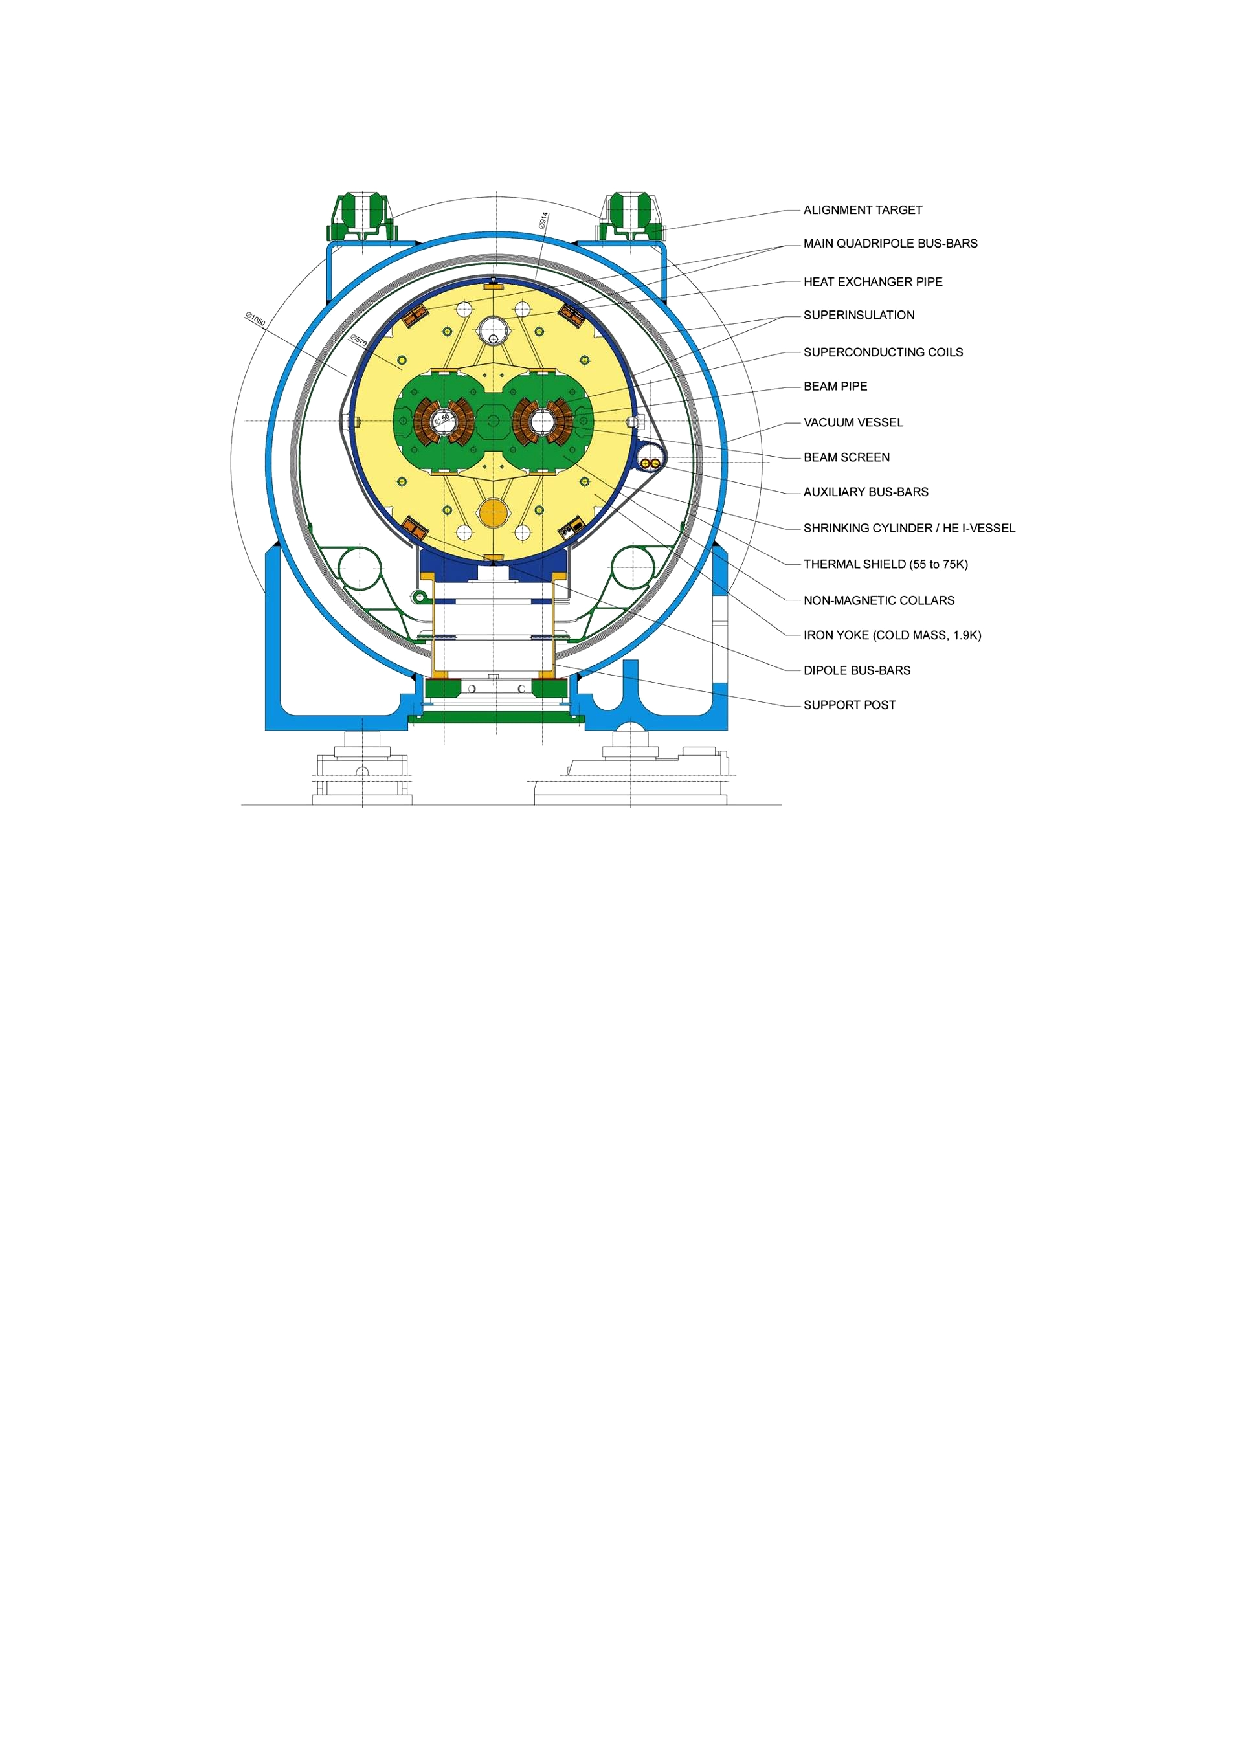
\includegraphics[width=0.7\textwidth]{Figures/LHC_magnet.pdf}
		%\rule{35em}{0.5pt}
	\caption[Schematics of dipole magnets]{Schematics of Dipole magnets}
	\label{fig:LHC_mag}
\end{figure}

%-----------------------------------
%	SECTION 2
%-----------------------------------

\section{Performance}

Since the start of the LHC in 2009, there were three years of machine operation, which yielded many physics results among which the discovery of Higgs boson reported by ATLAS and CMS collaborations. should be highlighted. First year of operation was devoted to commissioning and understanding machine characteristics with the emphasis on safety and testing machine protection systems. In 2011 new energy and instantaneous luminosity records were reached. These numbers were increased once again in 2012 with center of mass energy going to 8 TeV.
\par High bunch intensity with 50 ns bunch spacing was used in order to get a good instantaneous luminosity performance. This came at a cost of high number of collisions in one bunch crossing (pile-up) which was in 2012 around 12 collisions, and in some cases this number went as high as 20 interactions. With the increase of instantaneous luminosity in 2012, number of pile-up interactions was on the average around 30. Besides proton-proton collisions, LHC successfully delivered lead-lead ion runs in 2010 and 2011. primarily for the ALICE experiment, but also for CMS and ATLAS. At the start of 2013. there was also a successful proton-lead run performed for the first time. 

\begin{table}[h]
\centering
  \caption{LHC performance in 2012}
  \begin{tabular}{ l  c  c }
      \hline
      \hline
      Parameter & Design value & Value in 2012 \\
      \hline
      Beam energy [TeV] & 7 & 4 \\
      Bunch spacing [ns] & 25 & 50 \\
      Number of bunches & 2808 & 1374 \\
      Protons per bunch & 1.15$\times 10^{11}$ & 1.6-1.7$\times 10^{11}$ \\
      Peak luminosity [cm$^{-2}$s$^{-1}$] & 1$\times 10^{34}$ & 7.7$\times 10^{33}$ \\
      Max. number of events per bunch crossing & 19 & $\approx 40$ \\
      Stored beam energy [MJ] & 362 & $\approx$ 140 \\
      \hline
      \hline 
  \end{tabular}
\end{table}

LHC head achieved very good luminosity performance during pat years mainly because of the excellent beam quality delivered by the injectors with significantly more protons than nominal and with lower emittances. Since the LHC was capable to absorb these beams, it was chosen to continue to operate with 50 ns bunch spacing. This meant higher pile-up which had to be dealt with by the experiments. 


\begin{table}[h]
\centering
  \caption{LHC performance highlights}
  \begin{tabular}{ l  c }
      \hline
      \hline
      Max. luminosity delivered in one fill & 237 pb$^{-1}$  \\
      Max. luminosity delivered in 7 days & 1.35 fb$^{-1}$  \\
      Longest time in stable beams (2012) & 22.8 hours \\
      Longest time in stable beams over 7 days & 91.8 hours (55$\%$) \\
      \hline
      \hline 
  \end{tabular}
\end{table}

\begin{figure}[htbp]
	\centering
		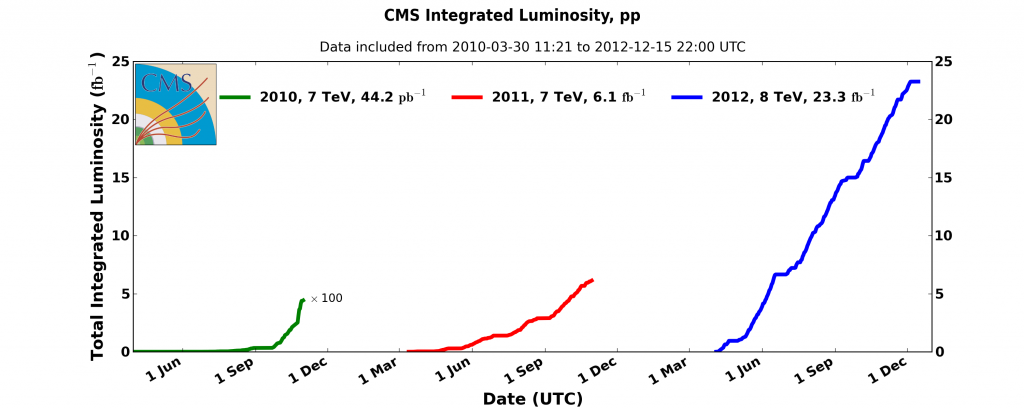
\includegraphics[width=0.7\textwidth]{Figures/lumi.png}
		%\rule{35em}{0.5pt}
	\caption[Luminosity delivered to the CMS experiment]{Luminosity delivered to the CMS experiment}
	\label{fig:LHC_lumi}
\end{figure}
 
Following a two year shutdown, LHC is anticipating operations at even higher energies of 6.5 TeV and later 7 TeV. The long term plan includes even higher peak luminosities, installation of the new injector complex and later the beginning of HL-LHC era. The timeline will, of course, be highly affected by the performance and results of the next run.
\chapter{The Compact muon solenoid} % Main chapter title

\label{Chapter4} % Change X to a consecutive number; for referencing this chapter elsewhere, use \ref{ChapterX}

\fancyhead[LE,RO]{Chapter 4. \emph{Compact Muon Solenoid}} % Change X to a consecutive number; this is for the header on each page - perhaps a shortened title

The Compact Muon Solenoid (CMS) is a general purpose detector designed to cover a wide range of physics topics at the LHC with a layered design approach and coverage of a large portion of the solid angle around the interaction point. The tracking system and calorimeters are placed inside a large soleonid in order to improve the resolution of the momentum and energy measurements. The detector outside the solenoid is aimed primarily to detection of muons. A drawing of the CMS detector is shown in Figure \ref{fig:CMS}. 
\begin{figure}[htbp]
	\centering
		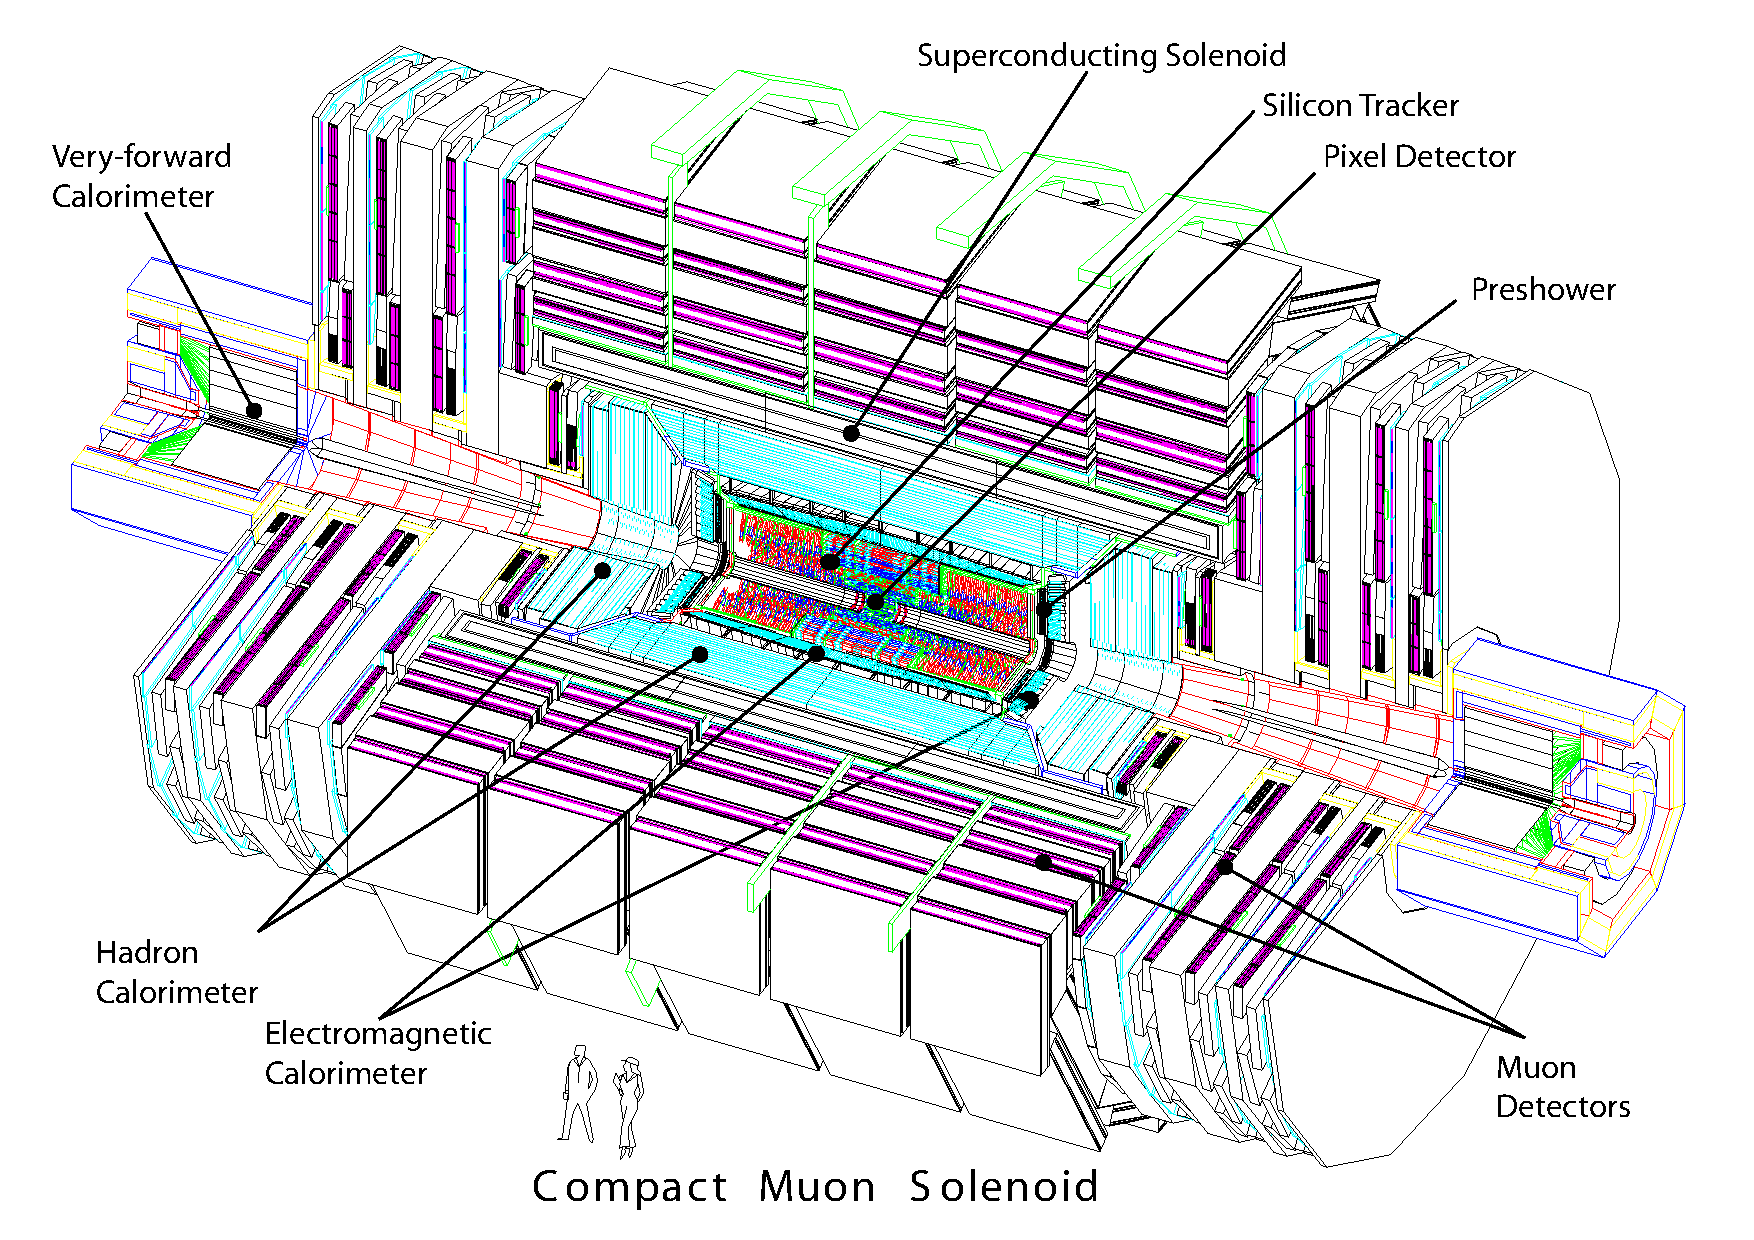
\includegraphics[width=0.9\textwidth]{Figures/CMS.pdf}
		%\rule{35em}{0.5pt}
	\caption[CMS detector]{A drawing of the CMS detector. \cite{Chatrchyan:2008aa}}
	\label{fig:CMS}
\end{figure}
\par The motivation for the CMS design with respect to its purpose in the LHC program is a very good muon identification and good momentum resolution over wide range of phase space and unambiguous determination of muon charge. Very good inner tracking system allows for detection of charged particles and high efficiency offline b quark and $\tau$ tagging. Other important requirements, specially for Higgs searches, is diphoton mass resolution, and photon and electron identification and isolation at high energies. 
CMS detector with its design meets all these requirements as is shown in following sections of this chapter. 

%----------------------------------------------------------------------------------------
%	SECTION 0
%----------------------------------------------------------------------------------------

\section{CMS coordinate system}

CMS uses a right-handed coordinate system with the origin in the nominal interaction point. $z-$axis is pointing along the beam line. $x-$axis is pointing towards the center of the LHC ring while y-axis points upwards. Two angles are used to describe position inside the detector, azimuthal angle $\phi$ and polar angle $\theta$. $\phi$ angle lies in $x-y$ plane with a range $[-\pi,\pi]$  and is defined as $\phi=$arctan$(y/x)$. The other angle $\theta$ is usually not used in high-energy physics because differences in $\theta$ are not Lorentz invariant.
The variable that is Lorentz invariant is rapidity:
\begin{equation}
y=\frac{1}{2}ln\left[ \frac{E+p_z}{E-p_z}\right]
\end{equation}
In high energy experiments in the relativistic limit where $E>>m$, a quantity called pseudorapidity is a good approximation of rapidity:
\begin{equation}
\eta = -ln \left[ tan \frac{\theta}{2} \right]
\end{equation}
The Lorentz invariance of pseudorapidity means that a measurement of $\Delta\eta$ between particles is not dependent on specifying a reference frame, such as the rest frame of a particle or the laboratory frame. The term "forward" direction refers to regions of the detector that are close to the beam axis, at high $|\eta|$. When the distinction between "forward" and "backward" is relevant, the former refers to the positive $z$-direction and the latter to the negative $z$-direction.
\par In proton-proton collisions, colliding objects are partons and gluons. Given the energy-momentum conservation and the fact that the proton momentum in the plane perpendicular to the beam axis is negligible, the momenta of the final state particles have to be balanced in the $x-y$ plane. This is why transverse momentum is often used in various analyses and is computed as $p_T=\sqrt{p_x^2+p_y^2}$.


%----------------------------------------------------------------------------------------
%	SECTION 1
%----------------------------------------------------------------------------------------

\section{Solenoid magnet}

The CMS solenoid magnet has the length of 12.9 m, an inner diameter of 5.9 m and provides a magnetic field of 3.8 T. The solenoid is large enough to contain inner tracking system and calorimeters  which reduces the material budget before the energy measurement in the calorimeters. The strong magnetic field increases the curvature of the trajectories of the highly energetic particles created in the collision thus improving the momentum resolution.
\par Solenoid magnet is built of superconducting materials with the operational temperature of 4.6 K. It is composed of four layers of superconducting material inserted in aluminum. Muon detectors outside the solenoid operate in 2 T magnetic field enhanced by the 10 000 t iron yoke.  

%----------------------------------------------------------------------------------------
%	SECTION 2
%----------------------------------------------------------------------------------------

\section{Inner tracker system}

The role of inner tracking system is to provide a precise measurement of the trajectories of charged particles with $p_T>1$ GeV and the pseudorapidity $|\eta|<2.5$. Additionally, it allows for precise secondary vertex positions reconstruction and impact parameter determination which allows for example to b-tag a jet. The size of CMS inner tracker is 5.8 m in length with a diameter of 2.5 m. Large magnetic field of 3.8 T is provided by the surrounding solenoid and is homogeneous across the entire inner tracking system. With the design LHC luminosity, expected occupancy of inner tracking system amounts to more than 1000 particles from 20 primary interactions in each bunch crossing. This requires high granularity detectors with fast responses and low dead time. In addition the amount of material in the detector has to be kept at minimum and the radiation hardness must be taken into account which lead to the solution of building an all-silicon detector with high granularity. CMS inner tracking system has two separate parts, Pixel detector and Strip detector, both described below.    


%-----------------------------------
%	SUBSECTION 2.1
%-----------------------------------
\subsection{Pixel Detector}

The pixel detector is the innermost part of the CMS, closest to the interaction point. The central part, called barrel pixel, consists of three layers located at radii of 4.4 cm, 7.3 cm and 11 cm. On each side of the barrel pixel, there are two discs at $z=$ 34.5 cm and 46.5 cm. The detector covers pseudorapidity range $-2.5<\eta<2.5$ which is illustrated in figure \ref{fig:pixels_eta}. Its purpose is to provide precise three dimensional space points for charged particle tracking and vertex position determination.
\begin{figure}[htbp]
	\centering
		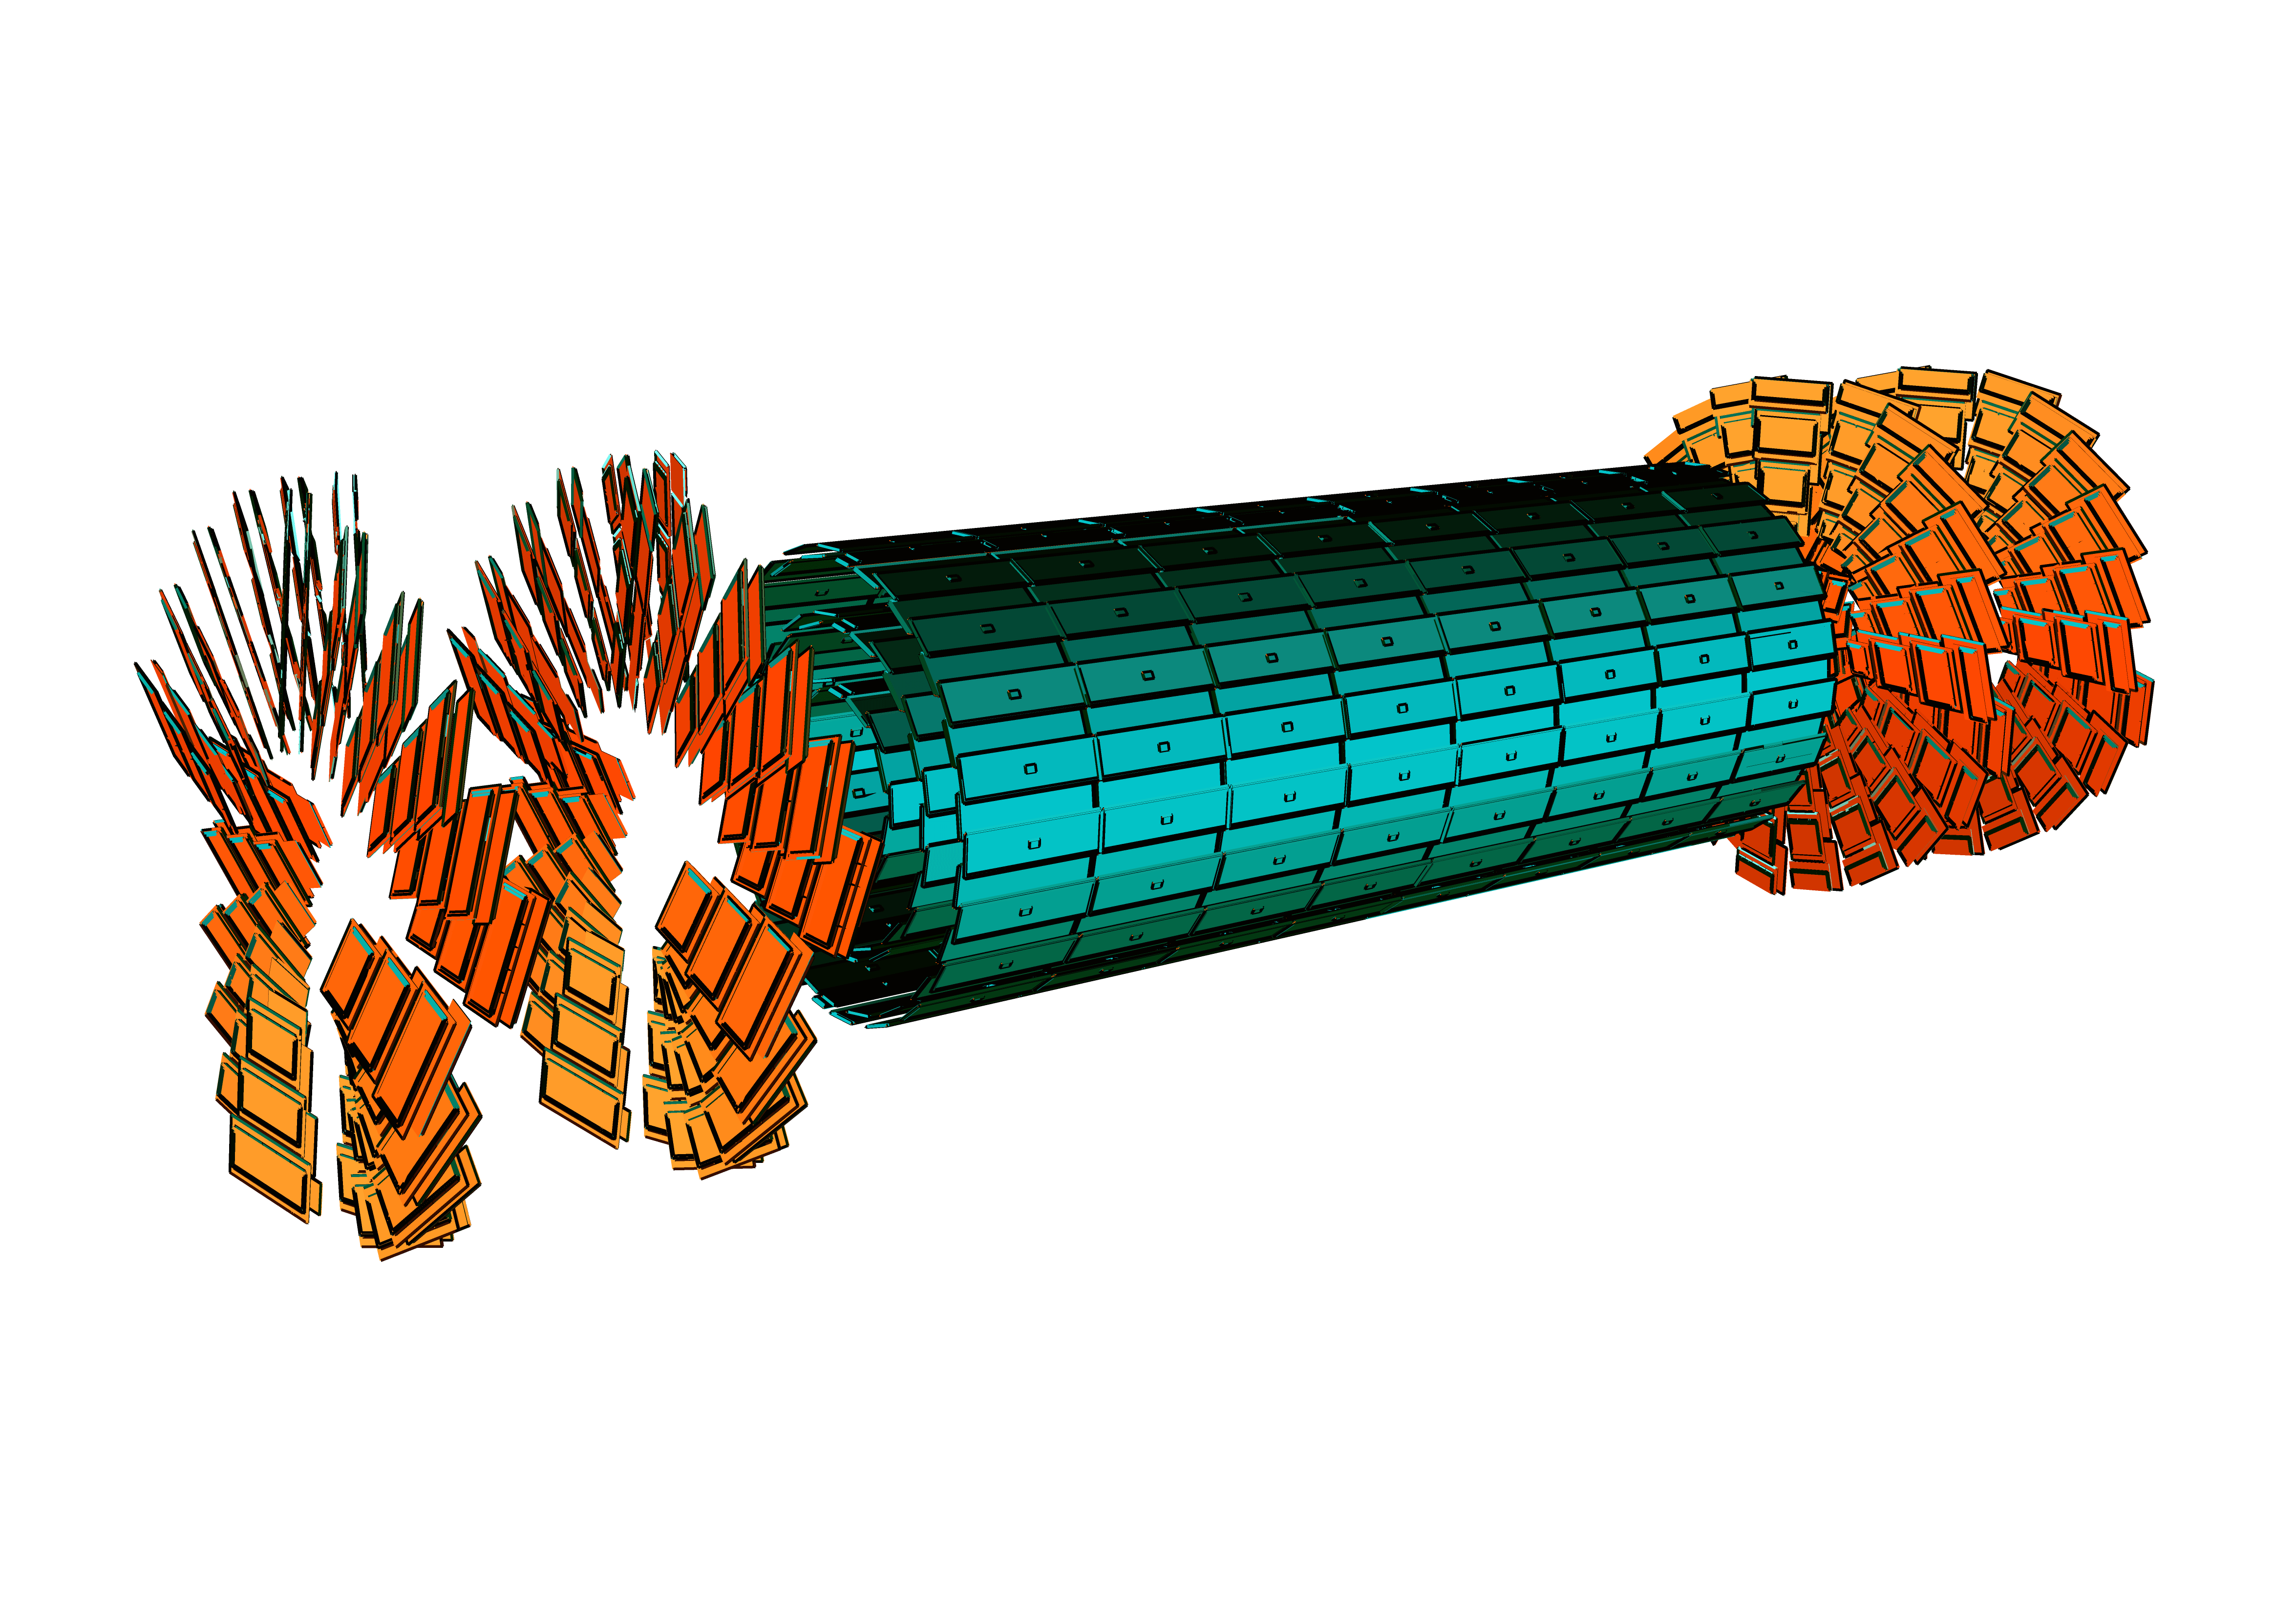
\includegraphics[width=0.8\textwidth]{Figures/pixel_detector.png}
		%\rule{35em}{0.5pt}
	\caption[CMS Pixel Detector]{A drawing of the CMS pixel detector. \cite{Chatrchyan:2008aa}}
	\label{fig:pixels}
\end{figure}
\begin{figure}[htbp]
	\centering
		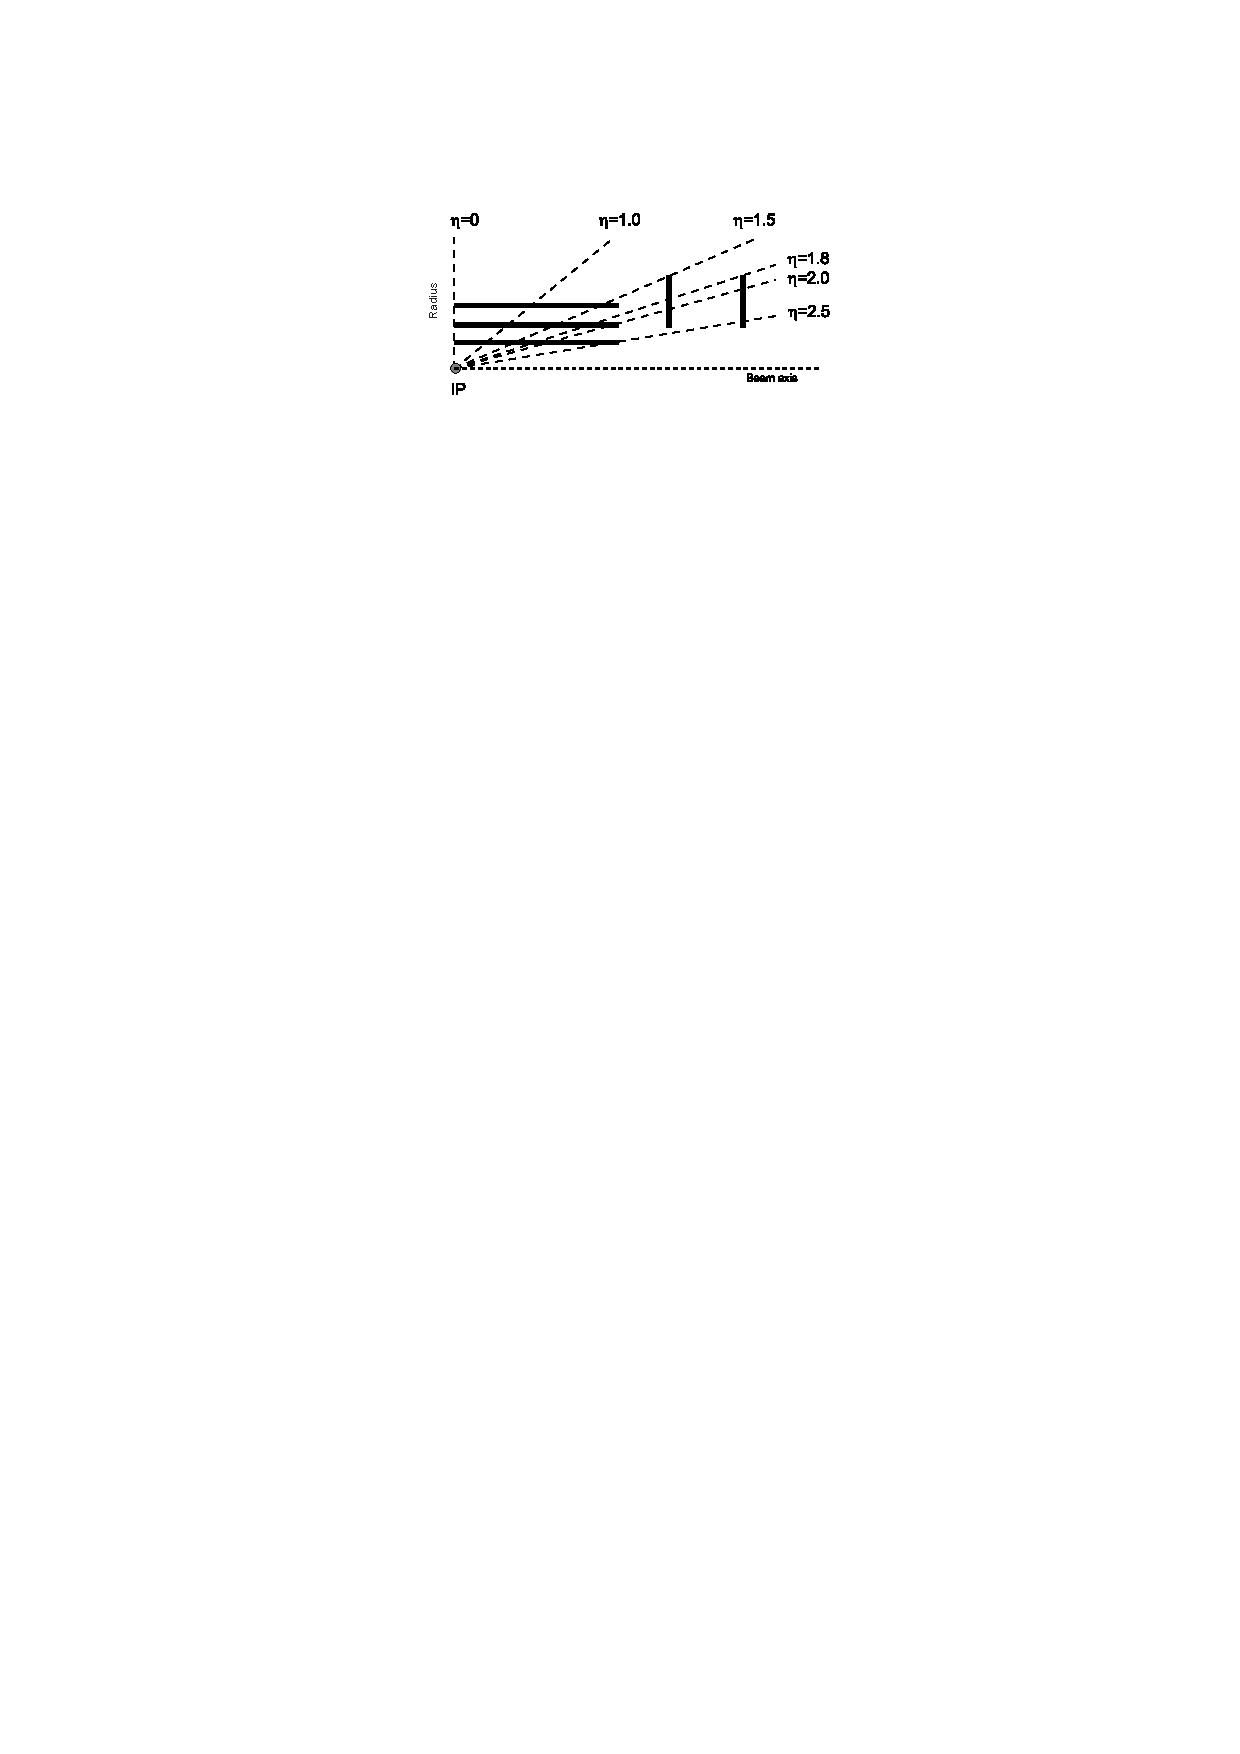
\includegraphics[width=0.49\textwidth]{Figures/pixel_eta.pdf}
		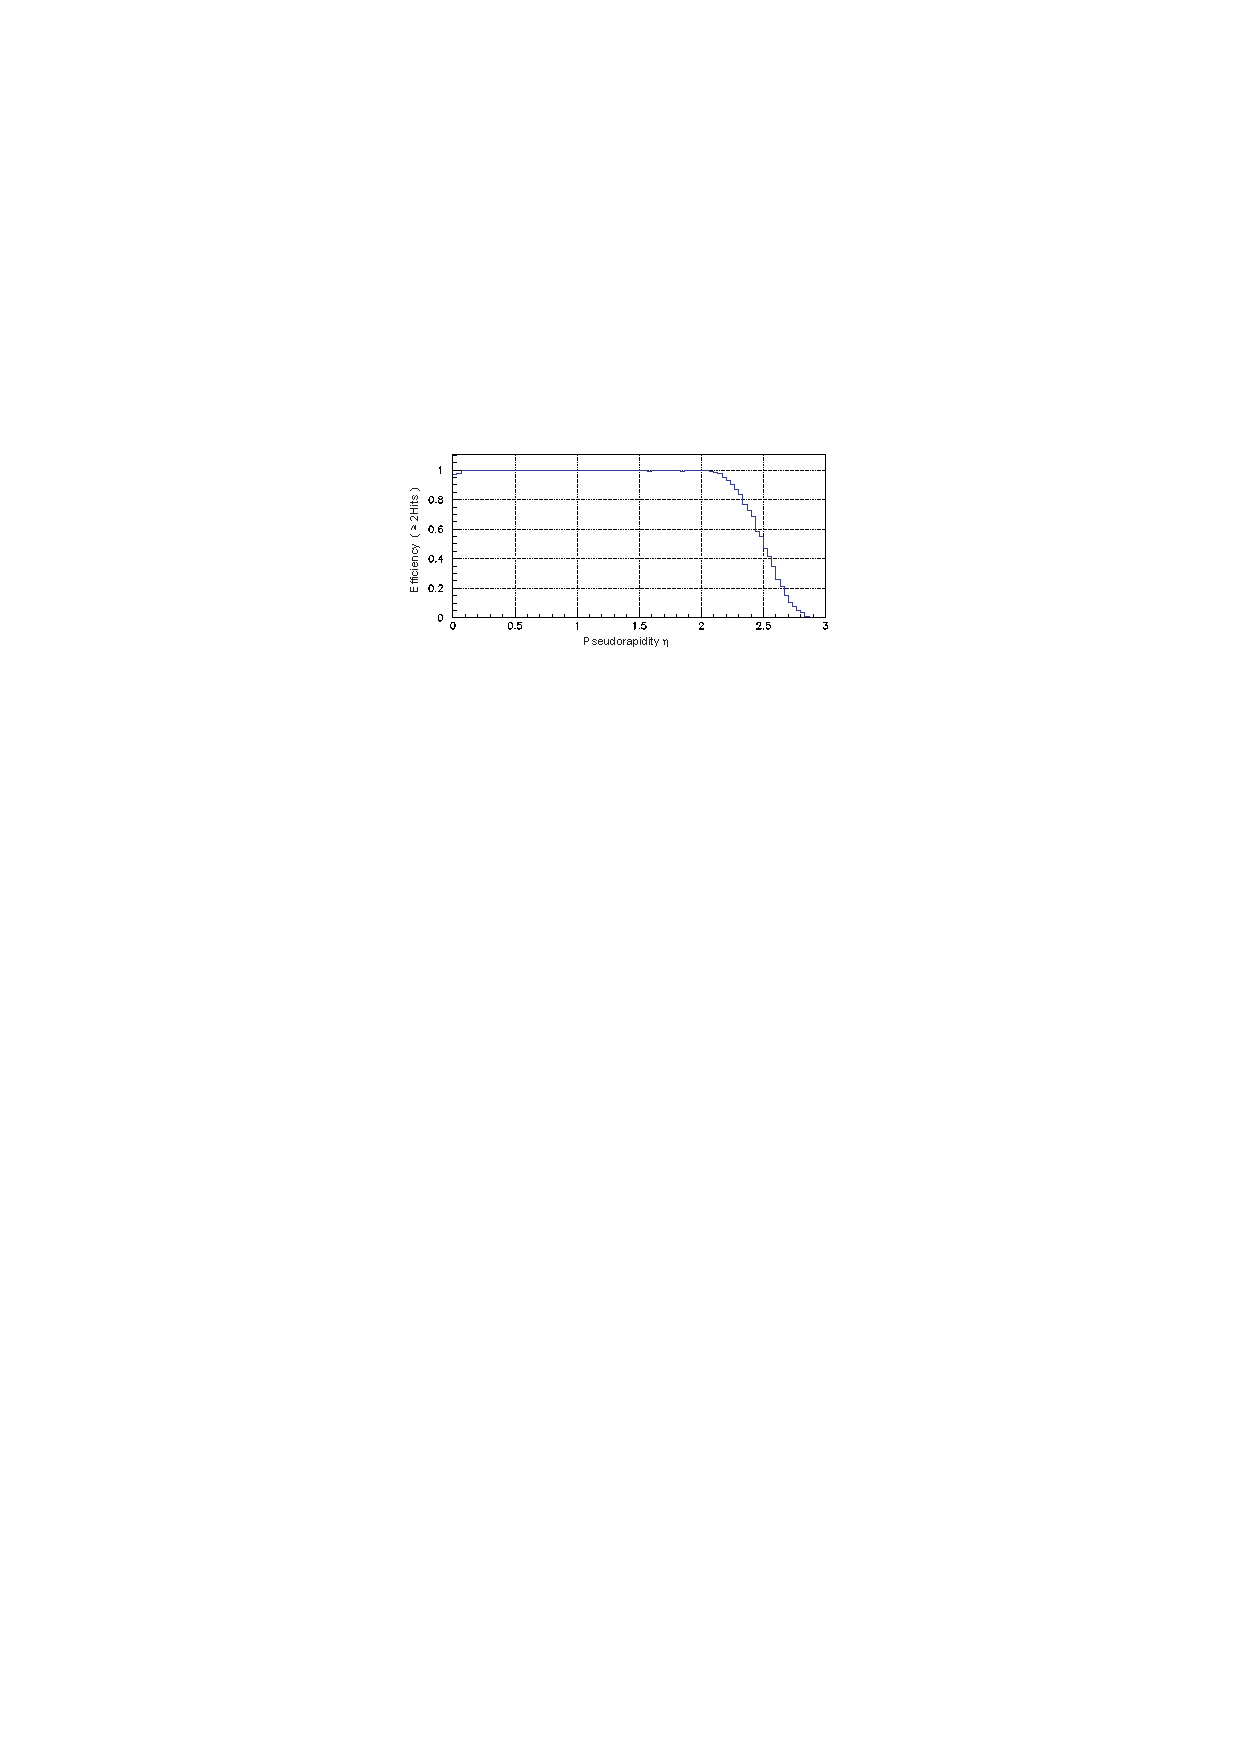
\includegraphics[width=0.49\textwidth]{Figures/pixel_eta2.pdf}
		%\rule{35em}{0.5pt}
	\caption[CMS Pixel Detector psudorapidity range coverage and efficiency]{A sketch of CMS Pixel Detector psudorapidity range coverage(\textit{left}) and hit efficiency as a function of pseudorapidity(\textit{right}). \cite{Chatrchyan:2008aa}}
	\label{fig:pixels_eta}
\end{figure}
\par Pixel detector is fully modular, consisting of rectangular modules in barrel part and quasi-triangular modules in the discs. Modules are arranged in a way to ensure measurements in at least three layers for each of the trajectories passing through the detector. Pixel size of $100\times150$ $\mu$m$^2$ results in similar resolution in $z$ and $r-\phi$ directions. In the barrel part the resolution of $15-20$ $\mu$m is achieved due to  charge sharing. Electrons inside the silicon shift under Lorentz force which is used in the reconstruction to determine the correct hit position. Detailed measurement of the Lorentz angle is described in the Appendix \ref{app:LA}. Pixel detector consists of 66 million pixels in total with 48 million being in the barrel pixel and 18 million in the forward. The closeness to the interaction point implies high track occupancy and necessity for radiation resistant materials. 
\par The readout of the pixel detector goes through read-out chips (ROC) to which each pixel is bump bonded and read out individually. There are around 16000 ROCs in the detector. Each ROC consists of 52$\times$80 pixels. Only pixels with signal above certain threshold are read out which can be tuned manually for each pixel. The average noise level in the detector is around 170 electrons at T$=-$10$^\circ$C. The information for each event is stored in a temporary buffer awaiting the signal from the Level-1 trigger in order to be read-out. Data is read out serially, with packets containing all hits corresponding to a single trigger. Each pixel hit uses six values, five to encode pixel position, and sixth value is the analog signal charge. ROC header is added at the beginning of each ROC sequence in order to make ROC hit-association possible. Signal is than digitized and sent to central data acquisition for further processing. Various other systems are installed in order to monitor and adjust the temperature, humidity, voltages, etc. 
\par With the design LHC luminosity, there are more than 1000 particles hitting the detector in every bunch-crossing. Very small pixel size results in the occupancy for each pixel of the order $10^{-4}$. The Pixel detector has been operational for several years and shows very little drop in performance due to irradiation. The plan is to keep the present detector during the Run 2, until 2017, and than replace it with new, four-layer pixel detector which is currently being built.

%-----------------------------------
%	SUBSECTION 2.2
%-----------------------------------

\subsection{Strip detector}

The silicon strip tracker is built in layers around Pixel detector where track particle flux is lower and a lower granularity detector can be used instead. The detector is built of strips in which a passing charged particle induces current. This resulting current is than transferred to silicon detectors connected to the wires. The barrel section of the strip detector consists of four layers in the inner part (TIB) and 6 layer in the outer part (TOB). In the forward regions there are three tracker inner discs (TID) on each side of the barrel and 9 layers in the tracker endcap (TEC). 
\par Some strips are built in double layers tilted against each other by an angle of 100 mrad to precisely measure the position of both $r\phi$ and $rz$ directions. The pitch size between strips varies from 80 $\mu m$ in the TIB to 184 $\mu$m in TOB and TEC. With the increasing distance from the interaction point, both strip pitch and strip length increase and sensor thickness becomes larger hence affecting the resolution.    

\begin{figure}[htbp]
	\centering
		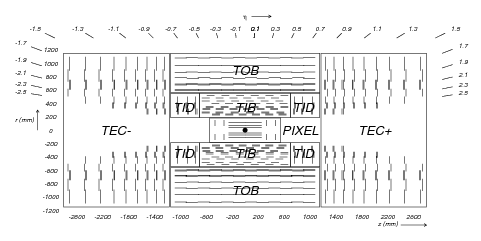
\includegraphics[width=0.9\textwidth]{Figures/strip_detector.png}
		%\rule{35em}{0.5pt}
	\caption[CMS Strip Detector]{A drawing of the CMS strip detector. \cite{Chatrchyan:2008aa}}
	\label{fig:strips}
\end{figure}

%----------------------------------------------------------------------------------------
%	SECTION 3
%----------------------------------------------------------------------------------------

\section{The electromagnetic calorimeter}

The electromagnetic calorimeter (ECAL) has the role of precisely measuring electrons and photons. It is built from lead tungstate (PbWO$_4$), a material with very high density (8.28 g$/$cm$^3$) and a small Moliere radius (0.89 cm) which is a scale characteristic of transverse dimension of the fully contained electromagnetic showers. The scintillation light emitted within a single bunch crossing of 25 ns is about 80$\%$ of the total light which means the response time of the detector is very small that represents a large advantage of this material. The calorimeters is built of 61 200 crystals in the barrel region and 14 670 crystals in the endcaps. Each crystal has a size of 22$\times $22 mm$^2$ in the front, 26$\times$26 mm$^2$ at the back side and length on 23 cm in the barrel region. In the endcaps, the size of the crystals varies from $28.62\times 28.62$ in the front to $30\times 30$ mm$^2$ in the back with a length of 22 cm. The whole systems covers the range $|\eta|<3$.
\begin{figure}[htbp]
	\centering
		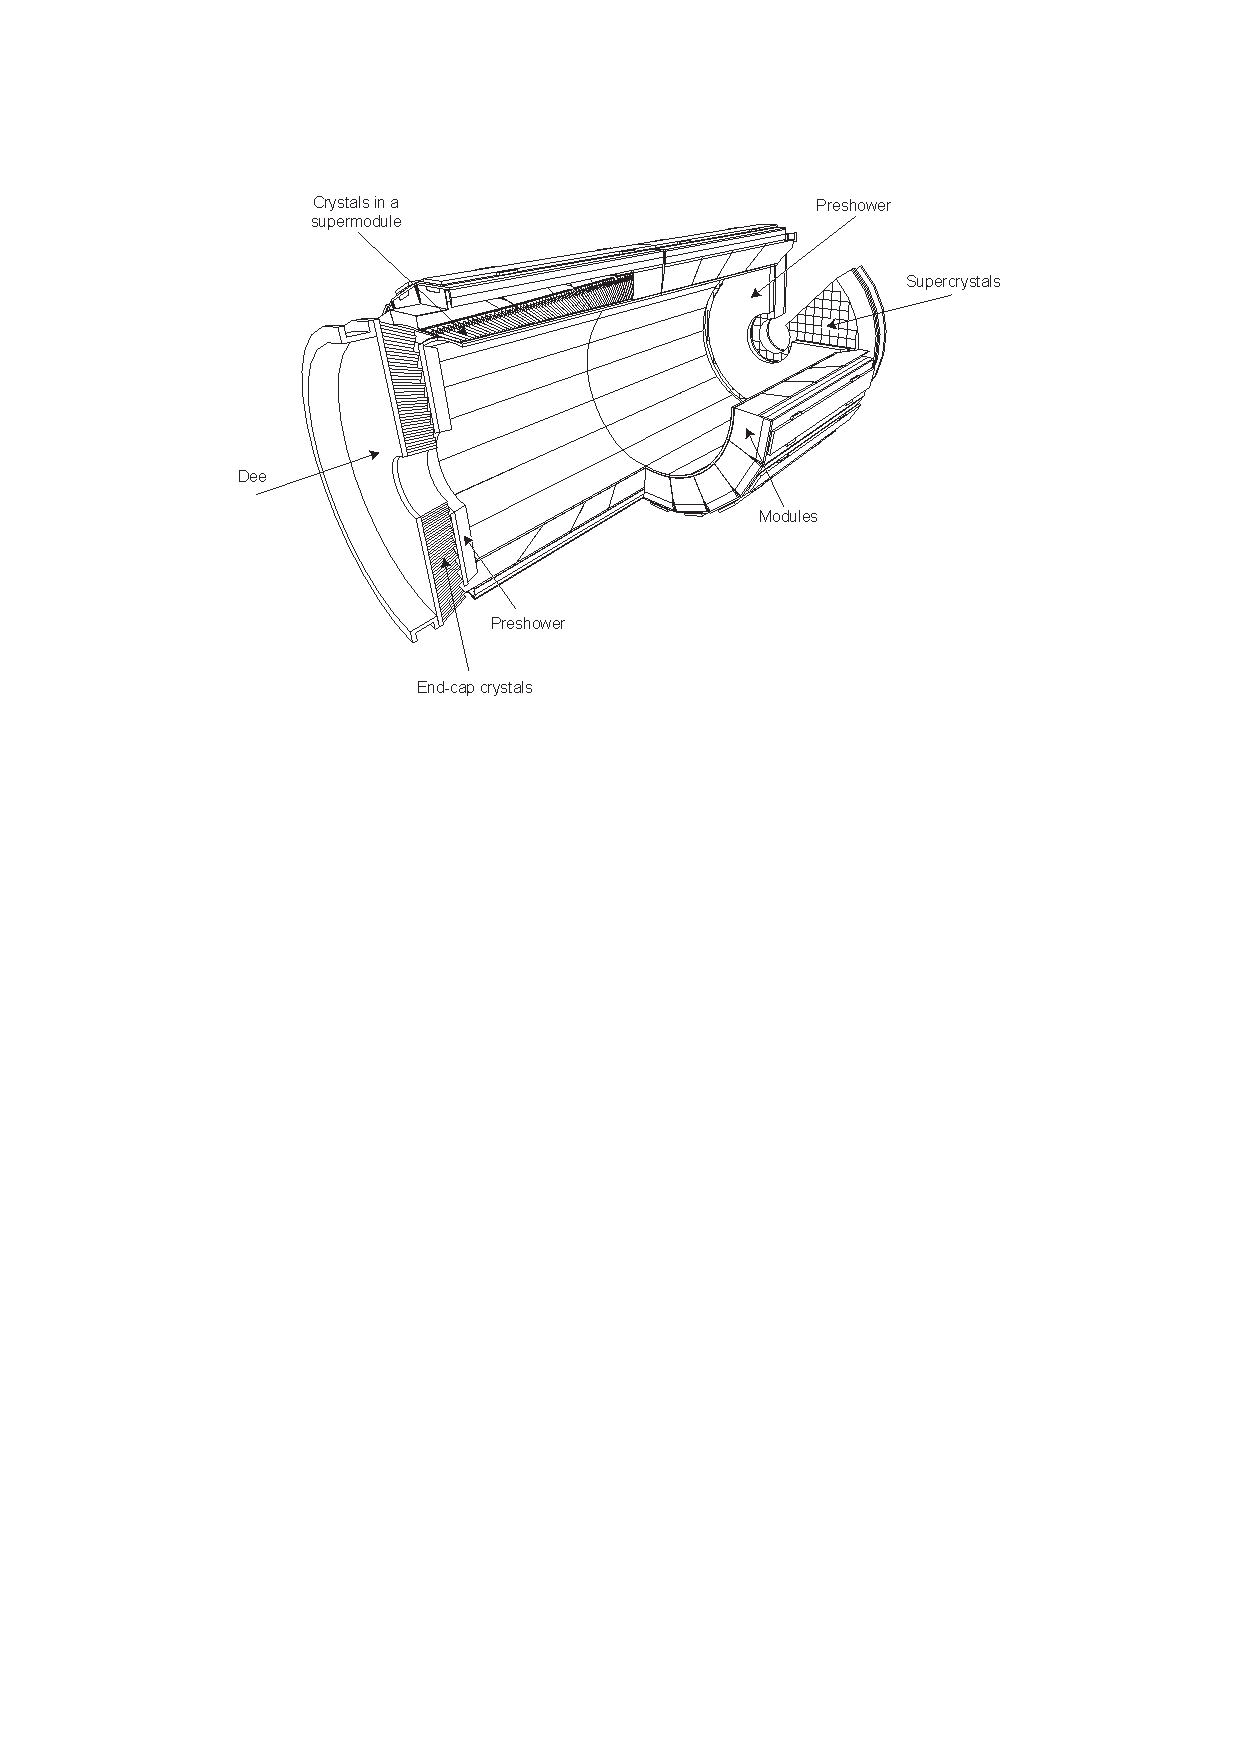
\includegraphics[width=0.8\textwidth]{Figures/ECAL.pdf}
		%\rule{35em}{0.5pt}
	\caption[CMS Electromagnetic Calorimeter]{A drawing of the CMS electromagnetic calorimeter. \cite{Chatrchyan:2008aa}}
	\label{fig:ECAL}
\end{figure}
\par Operation temperature of the detector is 18$^\circ$C at which $\sim$4.5 photoelectrons are collected per MeV of deposited energy. The blue-green scintillation light is measured by the avalanche photodiodes in the barrel and vacuum phototriodes in the endcaps.   
\par The ECAL energy resolution is affected by three uncorrelated sources and can be described by the relation \ref{eq:ECAL_res}. Parameters $a$, $b$ and $c$ are determined from the test beam. The stochastic term $a$ is very low for the lead tungstate crystals ($a$ = 2.83$\pm$0.3$\%$), which means that showers are mostly contained within the crystals. The noise term $b$ is determined from the electronics and amounts to $b=124$ MeV. The last term $c$ is the constant term which limits the ECAL accuracy at high energies.   
\begin{equation}
\left(\frac{\sigma_E}{E}\right)^2 = \left(\frac{a}{\sqrt{E}}\right)^2 + \left(\frac{b}{E}\right)^2 + c^2
\label{eq:ECAL_res}
\end{equation}   

%----------------------------------------------------------------------------------------
%	SECTION 4
%----------------------------------------------------------------------------------------

\section{The hadronic calorimeter}

The hadronic calorimeter (HCAL) is used to measure energies of hadron particles such as pions, kaons, protons, neutrons etc. Barrel and endcap hadronic calorimeters cover the pseudorapidity rande to $|\eta|=3$. 
Since the absorber in the transverse direction thickness is only 5.82 interaction lengths, additional layer was placed outside the solenoid and is called HO. HCAL is a sampling calorimeter which consists of layers of brass and plastic scintillator layers. Showers are produced mostly in brass and are detected in the scintillator and reemitted in the narrow wavelength range in which photodetectors operate. In the endcap region, steel and quartz are used because of their higher radiation hardness. There is an additional part of the detector placed 11.2 meters from the interaction point on both sides called forward HCAL which extends the coverage to $|\eta|=5.2$. Large HCAL coverage and good energy measurement are very important for jet reconstruction as well as for missing transverse energy determination.  
\begin{figure}[htbp]
	\centering
		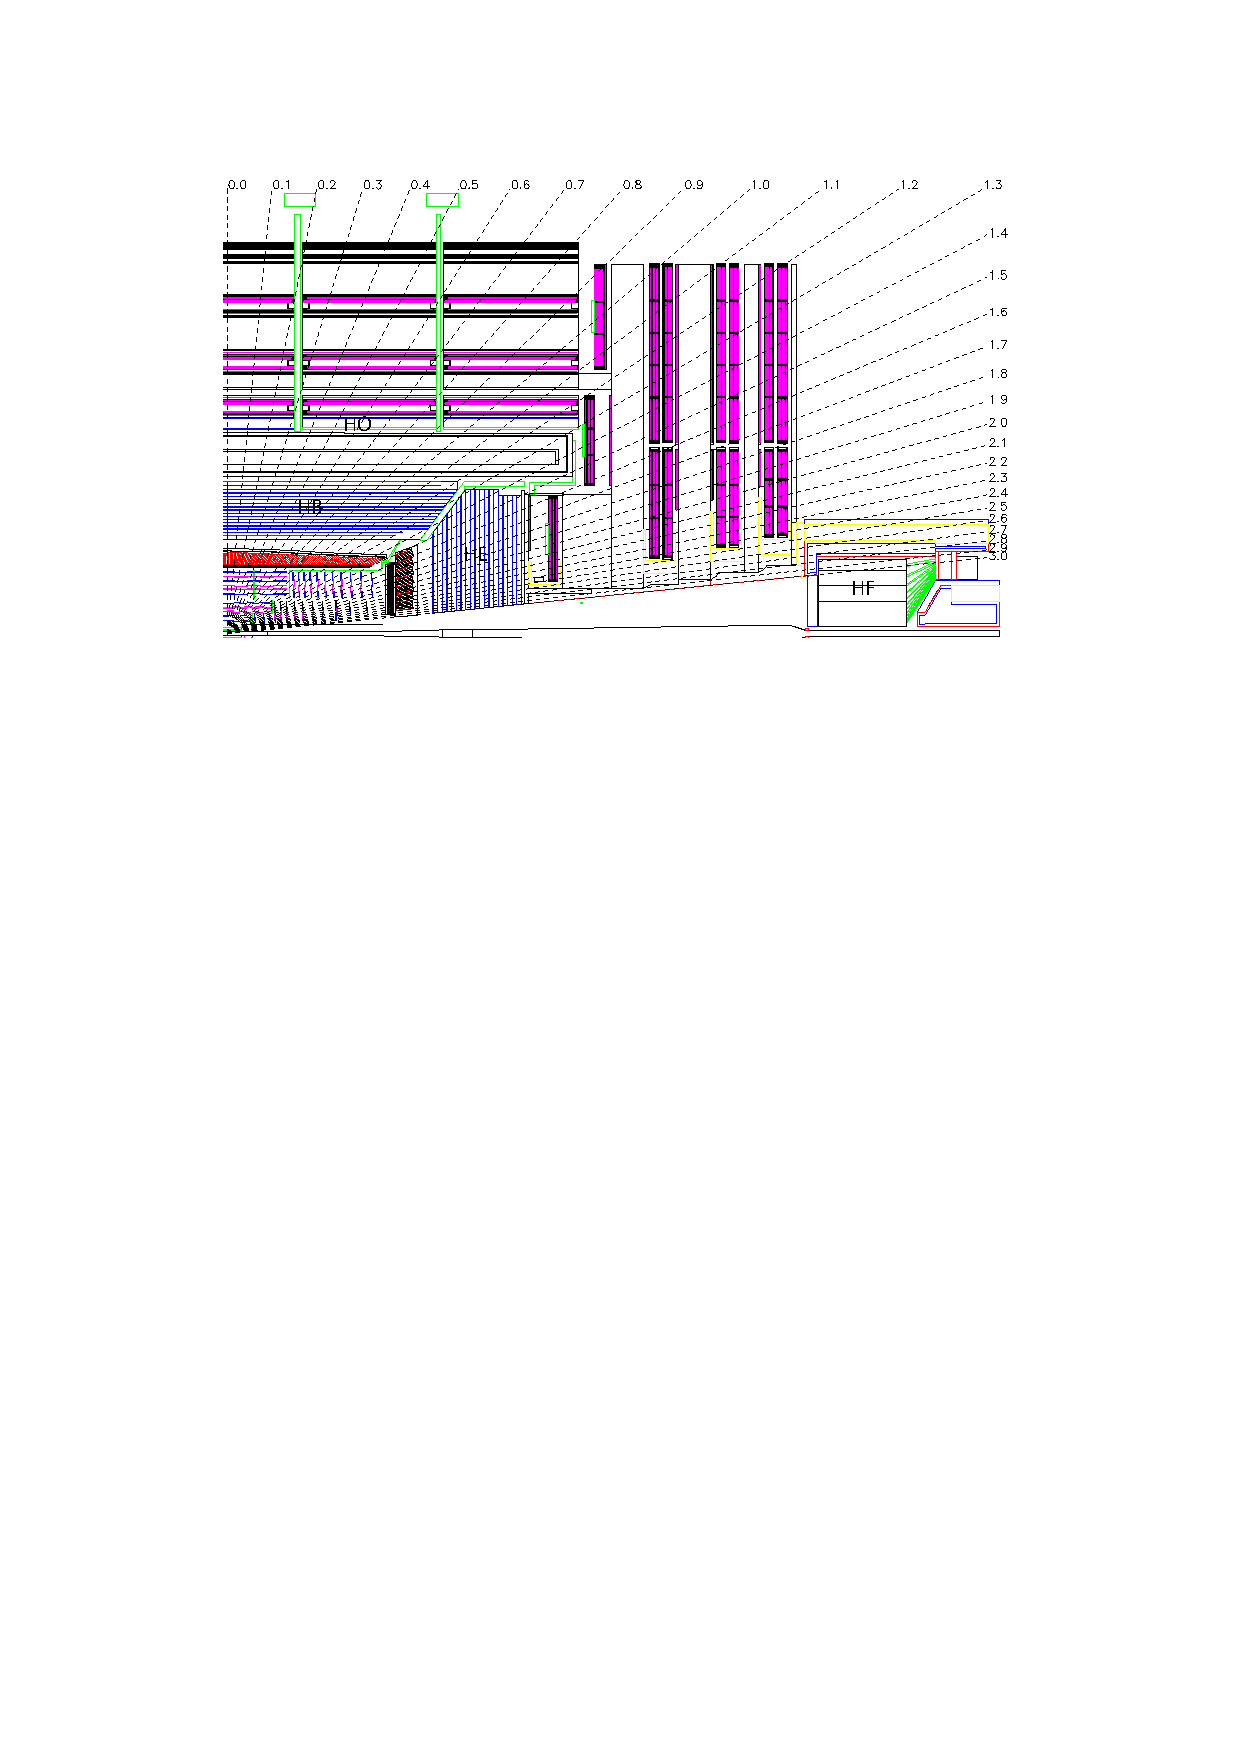
\includegraphics[width=0.8\textwidth]{Figures/HCAL.pdf}
		%\rule{35em}{0.5pt}
	\caption[CMS Hadronic Calorimeter]{A drawing of the CMS Hadronic Calorimeter. \cite{Chatrchyan:2008aa}}
	\label{fig:HCAL}
\end{figure}


%----------------------------------------------------------------------------------------
%	SECTION 5
%----------------------------------------------------------------------------------------

\section{The muon chambers}

Muons are the only particles that can pass the calorimeters and the solenoid. Their charge and momentum is measured also in the outer part of the detector by the muon chambers. There are three different types of the gaseous detectors used in the muon system, Drift tubes (DT), Resistive Plate Chambers (RPC) and Cathode Strip Chambers (CSC). Drift tubes are used in the barrel region where muon rate is relatively low and covers pseudorapidity range of $|\eta|<1.2$. The signal in Drift tubes is generated when a particle ionizes the gas inside the tube and the charge is collected by wires which are at high voltages. Cathode Strip Chambers are used in the endcap region where muon rate is much higher and magnetic field is not uniform. These are multi-wire proportional chambers with anodes that collect charge from the gas ionization. Resistive Plate Chambers are placed both in barrel and endcap region. These detectors are designed as two parallel plates which create a uniform electric field in the gas between them. The electrodes on the plates are highly resistive so  when charged particle passes, it causes an electron avalanche which passes through the plates and is collected by the external metallic strips. Their time resolution is of the order $\sim$1 ns which makes RPCs a good choice for triggering although their spatial resolution is not so good.
\begin{figure}[htbp]
	\centering
		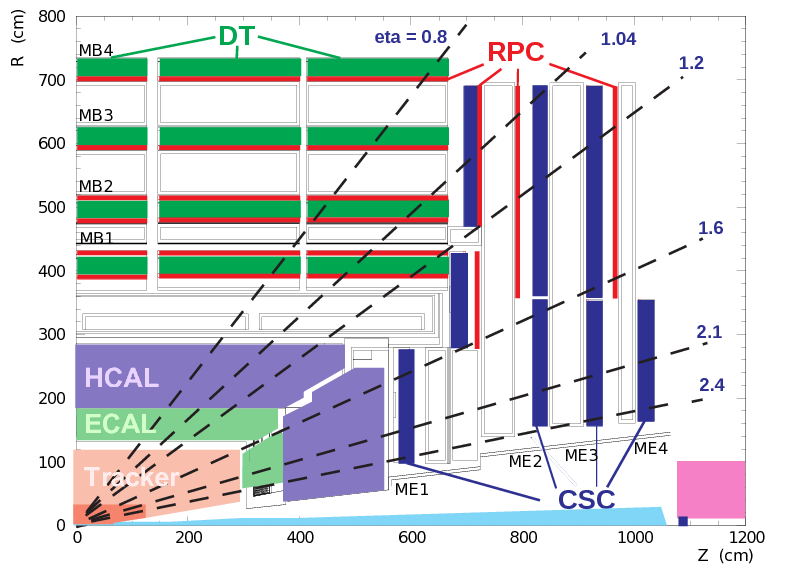
\includegraphics[width=0.8\textwidth]{Figures/Muon_chambres.png}
		%\rule{35em}{0.5pt}
	\caption[CMS Muon Chambers]{A drawing of the CMS muon chambers which consist of three different types of the detectors: Drift tubes, Cathode Strip Chambers and Resistive Plate chambers. \cite{Chatrchyan:2008aa}}
	\label{fig:Mu}
\end{figure} 
\par Large magnetic field enables even for high $p_T$ muons to be measured with a reasonable cell size in the muon chambers. The limiting factor for a good resolution of low $p_T$ muons is multiple scattering, and for high $p_T$ muons the chamber resolution. The momentum resolution as a function of muon $p_T$ is shown in Figure \ref{fig:MU_pt} for both muon chambers and inner tracking as well as the combined result. 
\begin{figure}[htbp]
	\centering
		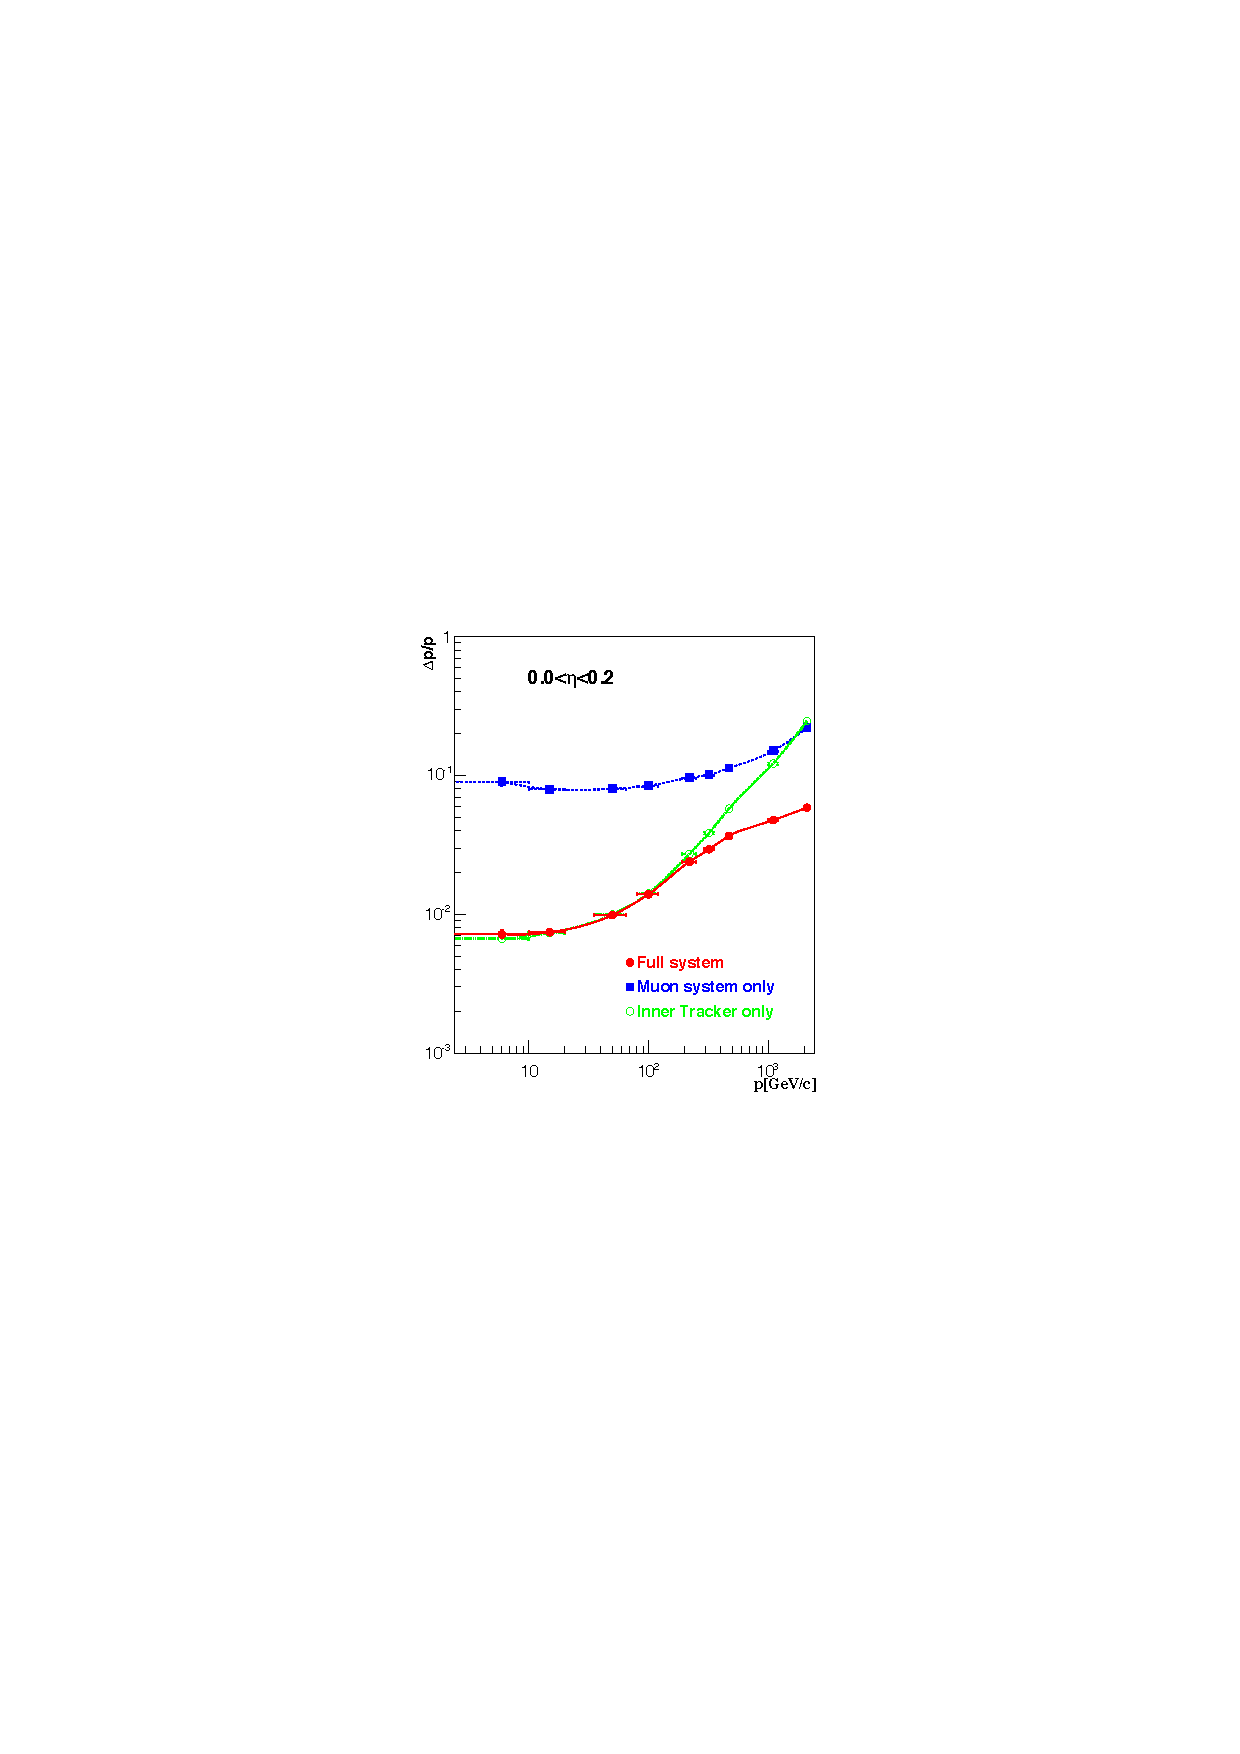
\includegraphics[width=0.5\textwidth]{Figures/MU_pt_res.pdf}
		%\rule{35em}{0.5pt}
	\caption[Muon resolution measurements for tracker, muon chambers and combined]{Muon resolution measurements for tracker, muon chambers and combined \cite{Chatrchyan:2008aa}}
	\label{fig:MU_pt}
\end{figure} 


%----------------------------------------------------------------------------------------
%	SECTION 6
%----------------------------------------------------------------------------------------

\section{The trigger}

The design rate of the proton collisions at the LHC is 40 MHz, although during Run 1 data taking period, the rate was 20 MHz which corresponds to 50 ns bunch spacing. Data collected in the same bunch crossing is called an event. Since there are huge amounts of data coming from the subdetectors, it is necessary to apply some selections which can reduce the rate to about 100 events per second. This is done by two level triggering system, the first one called Level 1 (L1) trigger and the second one called High Level Trigger (HLT). L1 trigger uses a special custom made electronics designed to reduce the output rate from 40 MHz to 100 kHz. Events which pass some loose criteria are than passed to the HLT. The L1 trigger uses the information from calorimeters and muon chambers to take the decision whether the event should be accepted or rejected usually searching for the presence of muons, jets above certain $p_T$, or looking at the total amount of $E_T$ and $E_T^{miss}$. The time needed to send the signals to the electronics, run the L1 selection and send the information back to the subdetectors in 3.2 $\mu$s. If the L1 trigger accepts the event, that is stored in the readout buffers where partial reconstruction takes place and the event is than processed by the HLT, which is a software farm that reduces the number of events to about 100 per second. The schematic of the trigger system is shown in figure \ref{fig:trigger}.
\begin{figure}[htbp]
	\centering
		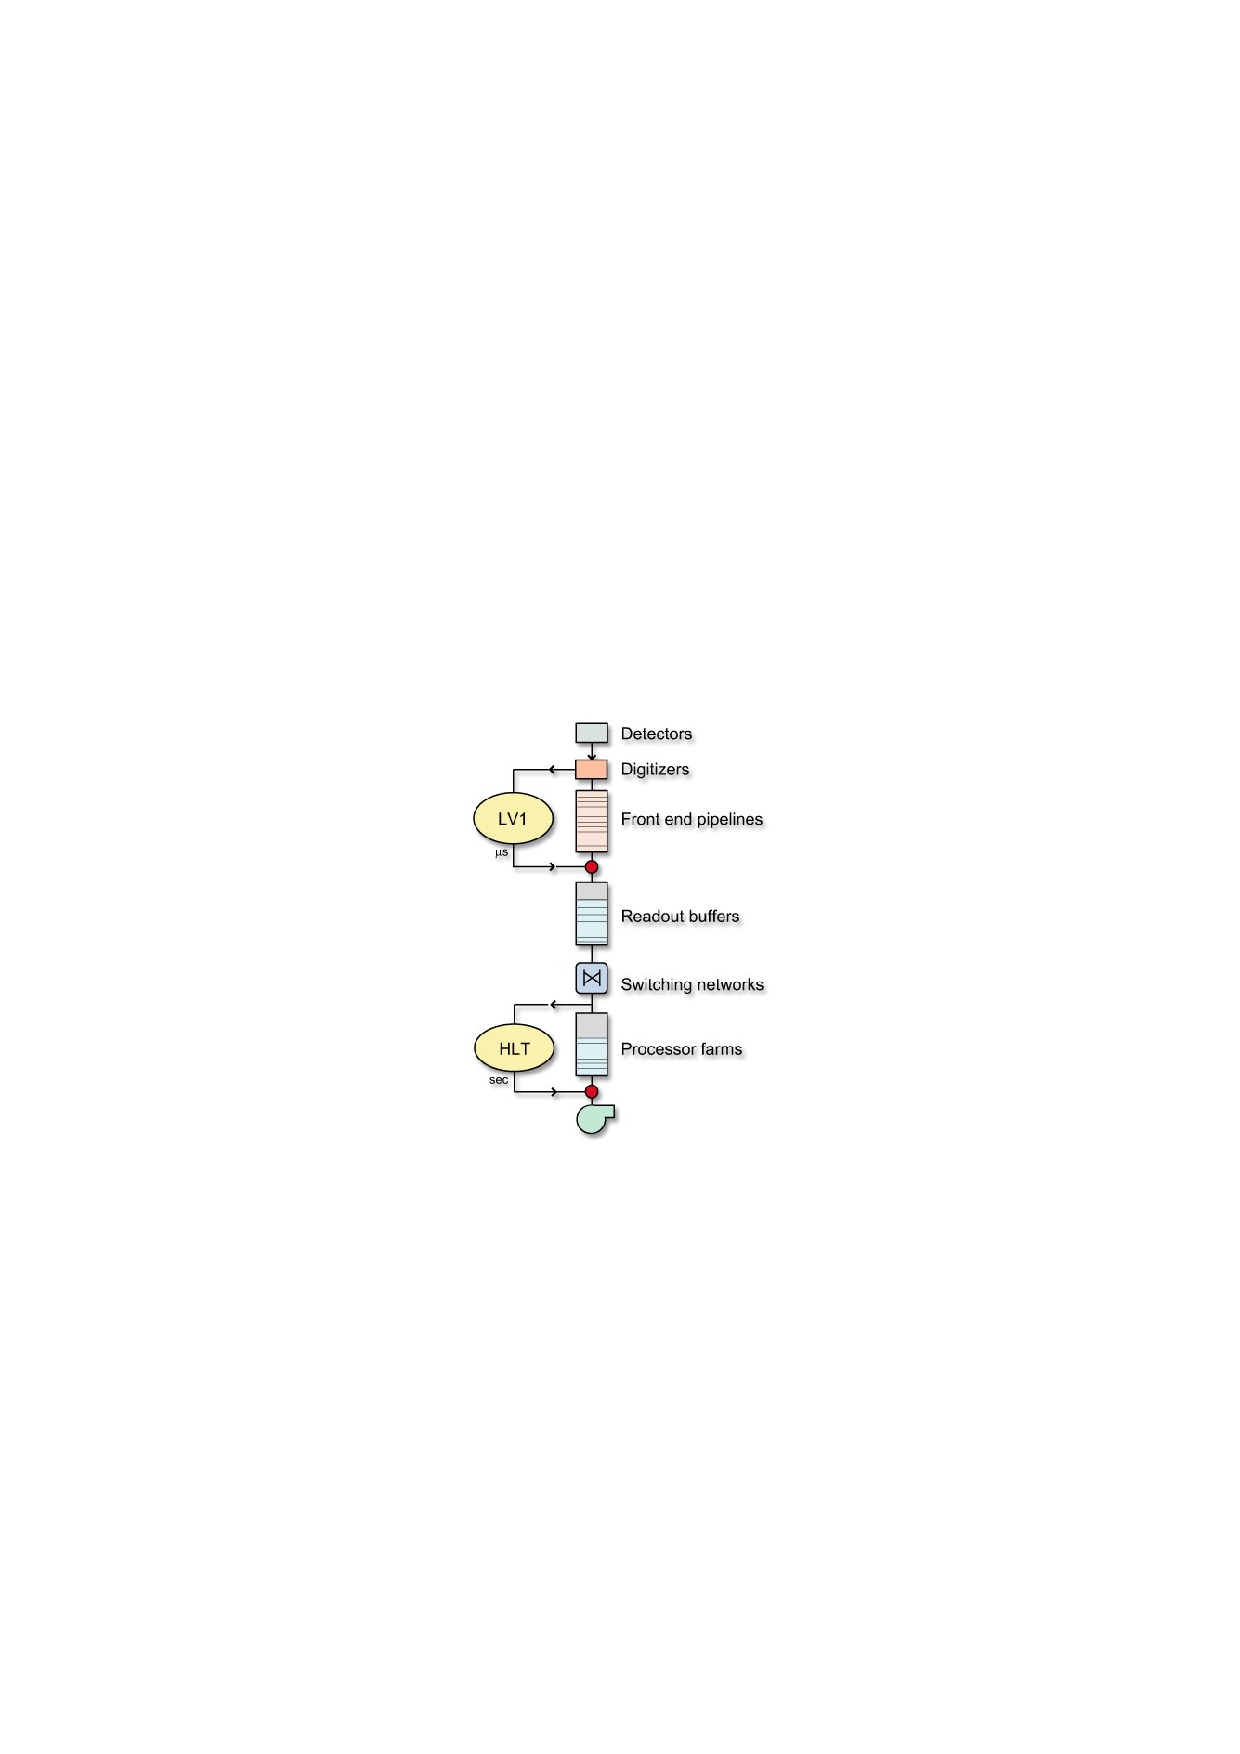
\includegraphics[width=0.4\textwidth]{Figures/trigger.pdf}
		%\rule{35em}{0.5pt}
	\caption[A drawing of CMS Trigger System.]{A schematic of CMS Trigger System. \cite{Chatrchyan:2008aa}}
	\label{fig:trigger}
\end{figure}

%----------------------------------------------------------------------------------------
%	SECTION 7
%----------------------------------------------------------------------------------------

\section{Luminosity measurement}
\label{sec:lumi}

Accurate and precise luminosity measurement is essential for physics analyses. CMS measurement is based either on the activity in the forward hadronic calorimeter (HF) or on the number of clusters in the pixel detector.
The forward calorimeter is placed in the high pseudorapidity region, covering range $3<|\eta|<5$. The measurement relies on the fraction of nonempty calorimeter towers to estimate the number of interactions. The uncertainty to this measurement comes from the nonlinear response of the HF to luminosity and the occurrence of the afterglow, the effect when the energy deposits created in a given bunch crossing produce a signal in subsequent bunch crossings. 
\par Luminosity measurement with the pixel detector is described in detail in \cite{CMS-PAS-SMP-12-008,CMS:2013gfa}. This method relies on the effective cross section measurement for pixel clusters determined with Van der Meer scan. This scan determines the shape and size of the interaction region by moving the beams across each other in transverse plane thus measuring the maximum available collision rate. The value of this cross section is then used to determine integrated luminosity for each lumi-section (23.3 seconds). This approach is not suitable for online luminosity measurements as pixel bias voltage is not turned on until the stable beams are declared and the data is not available if the central data acquisition system is busy. On the other hand, in the offline analysis this is not a problem as the data recorded without the pixel detector is discarded anyway.    
The total luminosity delivered in 2012 was around 24 fb$^{-1}$ while the luminosity recorded by the CMS was around 22 fb$^{-1}$. Ideally these two numbers would be the same, but due to the downtime of data acquisition or some of the subsystems, some of the delivered luminosity is not recorded.  
\chapter{Physics objects definitions} % Main chapter title

\label{Chapter5} % Change X to a consecutive number; for referencing this chapter elsewhere, use \ref{ChapterX}

\lhead{Chapter 5. \emph{Physics object definitions}} % Change X to a consecutive number; this is for the header on each page - perhaps a shortened title

CMS detector is designed to efficiently identify and reconstruct interesting physics objects. The reconstruction procedure which takes as input the signals from all subdetectors and combines them to get physics objects is called \textit{particle flow}. \cite{CMS:2009nxa} This algorithm classifies all the objects into one of the following categories: charged hadrons, neutral hadrons, photons, electrons and muons. These are built from reconstructed tracks, energy deposits in the calorimeters and signals in the muon chambers creating a global event description. Additionally, a set of cuts is imposed on both input signals and reconstructed object in order to minimize the misidentification, e.g wrongly identifying electron as a jet. 
\par Following sections show electron and muon reconstruction procedures and identification criteria. Additionally, jet reconstruction procedure is described together with necessary jet corrections and b-tagging algorithms. After the reconstruction of all other objects, missing transverse energy is computed.

%----------------------------------------------------------------------------------------
%	SECTION 1
%----------------------------------------------------------------------------------------

\section{Electrons}

Electrons in CMS are detected as a tracks in tracking system and an energy deposit in the electromagnetic calorimeter. Two different algorithms are used for electron reconstruction, \textit{tracker driven} seeding which is more suitable for low $p_T$ electrons and electrons inside jets and \textit{ECAL driven} seeding optimized for high $p_T$ isolated electrons. Both approaches take electromagnetic crystals with deposited energy and join them into \textit{clusters}. Electron passing through the detector bends due to magnetic field and interacts with the detector material emitting \textit{bremsstrahlung} photons. ECAL energy deposits from these photons are spread in $\phi$ direction in very narrow $\eta$ range and combined with the existing cluster forming a \textit{supercluster}. Trajectories are reconstructed using modeling of electron energy loss in detector material and fitted with a Gaussian Sum Filter(GSF)\cite{2005JPhG31N9A}.
\par Matching ECAL superclusters and reconstructed tracks is where the two approaches differ. Tracker driven seeding uses track from the tracking system and tries to match it with the supercluster in the ECAL while ECAL driven seeding starts from the superclusters.
Each electron candidate has to pass various quality cuts in order to maximize the probability of identifying the electron coming from the hard interaction, and reject electrons from jets or conversion. These selection cuts can be divided into three categories: identification, isolation and conversion cuts. Details on electron reconstruction and performance can be found in \cite{CMS:2010bta}.

%-----------------------------------
%	SUBSECTION 1.1
%-----------------------------------
\subsubsection*{Electron identification}
\label{sec:eleID}

Electron identification procedure first focuses on good matching between reconstructed track and supercluster, by imposing cuts on angular distance $\Delta \eta$ and $\Delta \phi$ between the two. These variables are computed as absolute $\eta$ and $\phi$ distance between the supercluster and electron track extrapolated to the ECAL surface. Additionally, a cut is imposed on $\sigma_{i\eta i\eta}$ which describes a shower shape spread in $\eta$ direction. This variable is particularly discriminating against clusters coming from electrons and energy deposits from photons and fakes. Shower shape is defined as:
\begin{equation}
\sigma_{i\eta i\eta} = \sqrt{\frac{\sum_{i}^{5\times 5} w_i(\eta_i-\eta_{seed})^2\times \Delta \eta^2_{xtal} }{\sum_{i}^{5\times 5}}}
\end{equation}
where $i$ runs over all crystals in $5\times5$ block around supercluster seed, $\eta_i-\eta_{seed}$ is the distance in number of crystals in $\eta$ direction between $i$-th crystal in supercluster and seed crystal and $\Delta \eta^2_{xtal}$ is the average width of a single crystal. Each crystal is given a weight defined as $w_i=max(0,4.7+ln(E_i/E_{5\times5}))$, where $E_i$ is a single crystal energy, and $E_{5\times 5}$ is the sum of energy deposits inside a 5$\times$5 crystal block. 
Additional cut on the ratio between the energy deposits in the hadronic and electromagnetic calorimeter for electrons is used to discard the events with significant hadron activity.
\par Electrons coming from photon conversions are rejected by requiring a hit in every layer of the inner tracking system. Additionally, for each electron track a fit is performed trying to combine it with another electron track under the hypothesis that both electrons originate from converted photon. Electron is selected only if this probability is sufficiently small. Electron compatibility with the primary vertex is estimated by looking at the impact parameters in both $xy$ and $z$ planes. Due to the gap in the electromagnetic calorimeter in 1.4442 $< |\eta| <$ 1.566, all electrons which have a supercluster position reconstructed in this range are rejected. A full list of identification criteria is summarized in Table \ref{tab:eleID}.
 \begin{table}[h]
\centering
  \caption{A summary of electron identification criteria.}
  \label{tab:eleID}
  \begin{tabular}{ l  c c}
      \hline
      \hline
      	Variable & Barrel & Endcap \\
      	\hline
    		$\Delta\eta$ $<$ &  0.004 & 0.005 \\
     	$\Delta\phi$ $<$ &  0.03 & 0.02 \\
     	$\sigma_{i\eta i\eta}$ $<$ & 0.01 & 0.03 \\
		$H/E$ $<$ & 0.12 & 0.10 \\
		$d_{xy}$ $<$ & 0.02 cm & 0.02 cm \\
		$d_{z}$ $<$  & 0.1 cm & 0.1 cm \\
		$(1/E - 1/p)$ $<$ & 0.05 & 0.05\\
		Missing hits  & 0 & 1 \\
		Vertex Fit Probability & $10^{-6}$ & $10^{-6}$ \\    	

      \hline
      \hline 
  \end{tabular}
\end{table}


%----------------------------------------------------------------------------------------
%	SECTION 2
%----------------------------------------------------------------------------------------

\section{Muons}

Muons in CMS are reconstructed by combining a reconstructed track inside the tracker(\textit{tracker track}) and track in muon chambers (\textit{standalone muon track}). Individual track segments in the muon chambers are fitted using Kalman fitter technique \cite{Fruhwirth1987444}  in order to obtain a standalone muon track. Similar as with electrons, two approaches are used for combining track from tracker and standalone track. 
\par \textit{Global muon reconstruction} approach uses a standalone muon track in the muon chambers and tries to find a matching tracker track by combining parameters of two tracks by projecting it to the common surface. This \textit{outside-in} approach uses Kalman fitter technique to combine these two objects in an object called \textit{global muon}. Muon momentum is then determined from this global muon track using all available systems which shows improved precision in comparison to other approaches.  
\par The second approach for muon reconstruction is \textit{tracker muon reconstruction} which starts from tracks inside the tracker with $p_T>0.5$ GeV/c and total momentum $p>2.5$ GeV/c as potential muon candidates. Extrapolation is than performed to the muon chambers taking into account the magnetic field, Coulomb scattering in the material and other energy losses. \textit{Tracker moun} is found if at least one muon segment matches the extrapolated track. The efficiency of the \textit{Tracker muon} reconstruction is higher for low energy muons than the efficiency for the global muons, because only a single muon segment in the muon chambers is required. For high energy muons where more there are more segments inside muon chambers, \textit{global muon} algorithm is designed to have high efficiency. Detailed muon reconstruction procedure is shown in \cite{2012JInst7P0002T}.    

%-----------------------------------
%	SUBSECTION 2.1
%-----------------------------------

\subsubsection*{Muon identification}
\label{sec:muID}

In this analysis \textit{particle flow} muon identification selection is applied to the \textit{global muons}. Selection is applied in order to minimize misidentification of charged hadrons as muons, maximize the efficiency of muon identification inside jets and ensure good momentum measurement. Muons used in the analysis have $|\eta|<2.1$ and transverse momentum $p_T>30$ GeV with more than 5 hits in the inner tracker system and at least one hit in pixel detector. At least one good muon chamber hit in the \textit{global muon} track fit is required to have $\chi^2/ndof<10$, at least two segments in two different muon stations should be matched to a track in order to suppress muons from in-flight decays. Cosmic muons are rejected by applying cuts on the impact parameter with respect to the primary vertex of $|d_{xy}|<$0.2 cm and $|d_z|<$ 0.5 cm. Muon identification criteria are summarized in Table \ref{tab:muID}.

  \begin{table}[h]
\centering
  \caption{A summary of muon identification criteria.}
  \label{tab:muID}
  \begin{tabular}{ l  c c}
      \hline
      \hline
      	Variable & Requirement \\
      	\hline
    		number of pixel hits $>$ &  0 \\
     	number of inner tracker hits $>$ &  5 \\
     	$\chi^2/ndof$ $<$ & 10 \\
		number of muon hits $>$ & 0  \\
		chambers with matched segments $>$ & 1  \\		
		$d_{xy}$ $<$ & 0.2 cm \\
		$d_{z}$ $<$  & 0.5 cm \\
      \hline
      \hline 
  \end{tabular}
\end{table}
 

%-----------------------------------
%	SUBSECTION 2.2
%-----------------------------------

\section{Lepton isolation}
Leptons from W decays are in general expected to be well isolated. The degree of isolation is calculated using \textit{particle flow} approach by summing the transverse momenta contributions of particles around the lepton inside a specific cone. All charged particles are considered as well as photons and neutral hadrons with $p_T>$0.5 GeV. The cone used for determination of energy deposits is defined as $\Delta R = \sqrt{\Delta \phi^2+ \Delta \eta^2}$ around the lepton axis and isolation measure is defined as:
\begin{equation}
I_{PF}^{rel} = \frac{\sum p_T^{charged} + max(0, \sum E_T^{\gamma}+\sum E_T^{neutral}-0.5\sum E_T^{PU})}{p_T^l}
\end{equation}
where $p_T^{charged}$ is the sum of the momenta of charged hadrons and $E_T^{\gamma} $ and $E_T^{neutral}$ are the sums of photon and neutral hadron momenta. $E_T^{PU}$ is the sum of the pile-up transverse energies from neutral particles and is calculated as a sum of track transverse momenta not coming from the primary vertex inside the isolation cone. This is divided by the factor of 0.5 which corresponds approximately to the ratio of neutral to charged hadron production in the hadronization process of pile-up interactions. Selected muons are required to pass isolation cut $I_{rel}^{PF}<0.12$. On the other hand, if there is a requirement that there be no leptons in the event, the isolation cut is $I_{PF}^{rel}<0.2$. Electron isolation is computed in the same way with cut of $I_{rel}^{PF}<0.1$ for selected electrons and $I_{rel}^{PF}<0.15$ for vetoed additional electrons.


%----------------------------------------------------------------------------------------
%	SECTION 3
%----------------------------------------------------------------------------------------

\section{Jets}

In high energy physics, jet is a collimated group of hadrons which emerges as a result of quark or gluon fragmentation and hadronization process. Hadrons reconstructed in a particle detector need to be combined in order to form a jet and give information about the initial parton. A set of rules has to be created which define how to group particles and how to assign momentum to the jet. Usually this is done by summing the four-momentum of each particle in a jet.

%-----------------------------------
%	SUBSECTION 3.1
%-----------------------------------

\subsection{Jet algorithms}

Jet algorithms take into account the distance between particles and define rules to determine which particle belongs to what jet. Same jet algorithms should be applicable to both, experimental data and theoretical calculation.  Other important properties of jet algorithms are \textit{infrared safety} and \textit{collinear safety} which means if an event is modified by addition of soft emission of collinear splitting, the final number of hard jets will remain unchanged. These two properties together are called \textit{IRC safety}. IRC unsafe jet algorithms may break the cancellation of divergences by yielding one set of jets for tree-level splitting while loop diagrams lead to another, as shown if figure \ref{fig:jet_unsafe}, giving infinite cross-sections in the final calculations. Jet definitions, jet relation to partons and an overview of different jet algorithms are summarized in \cite{Salam:2009jx}.
\begin{figure}[htbp]
	\centering
		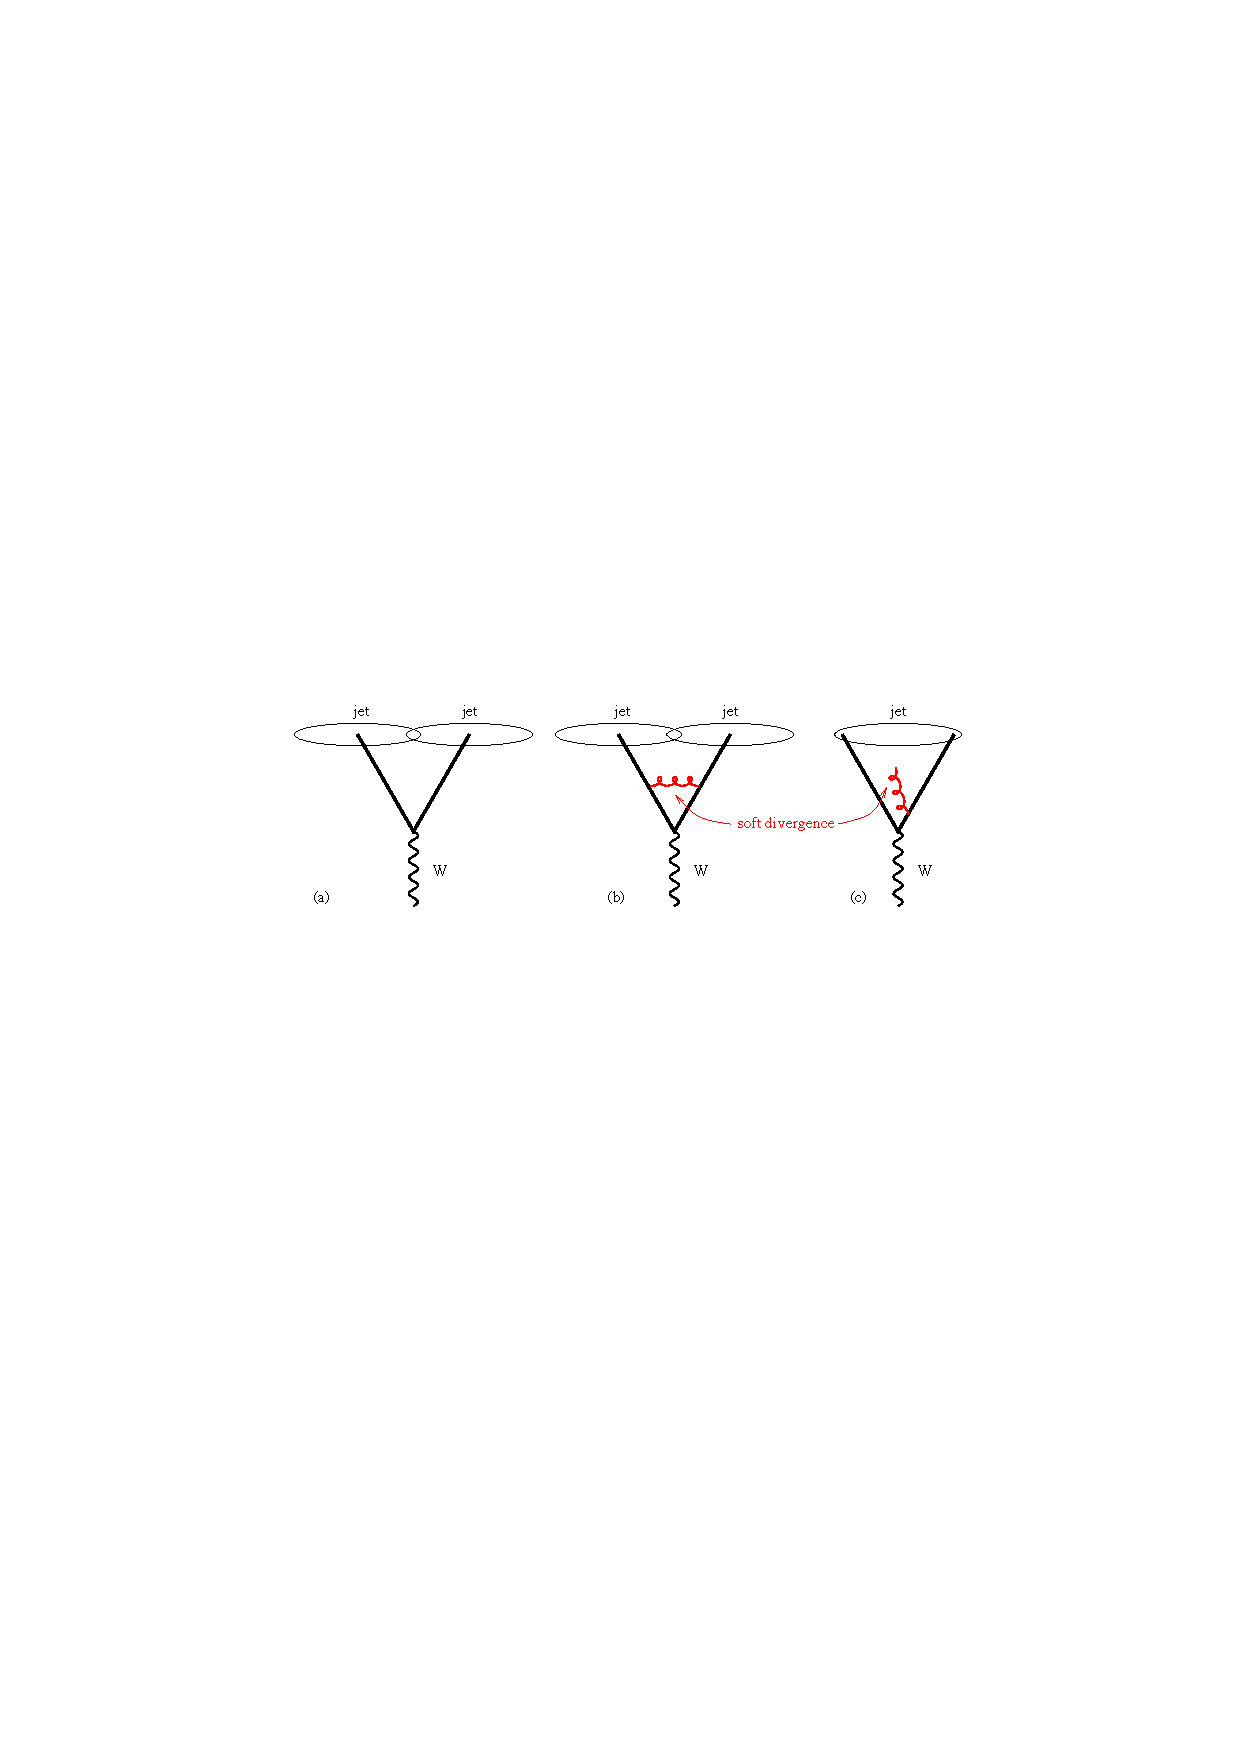
\includegraphics[width=0.8\textwidth]{Figures/jet_unsafe2.pdf}
		%\rule{35em}{0.5pt}
	\caption[An example of configuration of IRC unsafe jet algorithm.]{Configuration showing IC  unsafety with W boson and two partons. Adding a soft gluon causes two jets to be reconstructed as one. \cite{Salam:2009jx}}
	\label{fig:jet_unsafe}
\end{figure}

\par There are two types of jet algorithms which are most commonly used: \textit{cone algorithms} and \textit{sequential recombination algorithms}. In the case of \textit{cone algorithms}, a jet is defined as a set of particles inside a stable cone around their center of mass. Most popular cone algorithm is \textit{iterative cones} (IC) where a seed particle is chosen and momenta of all particles around that initial particle inside a cone of radius $R$ are summed. After adding each new particle to the sum, the direction of the new sum is taken as a seed direction, and the procedure repeats until the direction of the resulting cone is stable. Particles inside the cone are than removed from the list of available particles and the procedure repeats. This approach is not IRC safe given that nearly collinear splitting of the hardest particle in the event can be reconstructed as two jets. In that case, a less energetic, particle, pointing in another direction, can become the hardest particle in the event, yielding different set of jets. Cone algorithms can be IRC safe using a \textit{seedless cone} (SC) algorithm where all stable cone solutions are identified at once. However this approach is very time consuming even for small number of particles and thus very impractical to use.
In the \textit{sequential recombination algorithms} at hadron colliders two longitudinally invariant distances are introduced: $d_{ij}$ which is the distance between each pair of particles and $d_{iB}$ which is the particle-beam distance. These distances are defined as: 
\begin{equation}
d_{ij} = min(k_{T,i}^{2p},k_{T,j}^{2p}) \frac{\Delta R_{ij}^2}{R^2}
\end{equation}
\begin{equation}
d_{iB}=k_{T,i}^{2p}
\end{equation}
where $\Delta R_{ij}$ denotes the distance in the $\eta -\phi$ plane and is computed as $$\Delta R_{ij}^2 = (\eta_i-\eta_j)^2+(\phi_i-\phi_j)^2.$$ $k_T$ is transverse momentum of the particle, $R$ is an angular cut-off similar to the one in \textit{cone algorithms},  and $p$ defines which particles are clustered first and is described below. Both $R$ and $p$ are free parameters of the algorithm. The algorithm is applied using the following approach: first two distances $d_{ij}$ and $d_iB$ are computed and minimal values are found. If $d_{ij}$ is smaller, that two particles are combined, treated as a new particle and the distance with next particle in the list is computed. In case of $d_iB$ being smaller, $i$ is declared to be the final jet is removed from the list of particles. The procedure continues until there are no more particles in the list.
\begin{figure}[htbp]
	\centering
		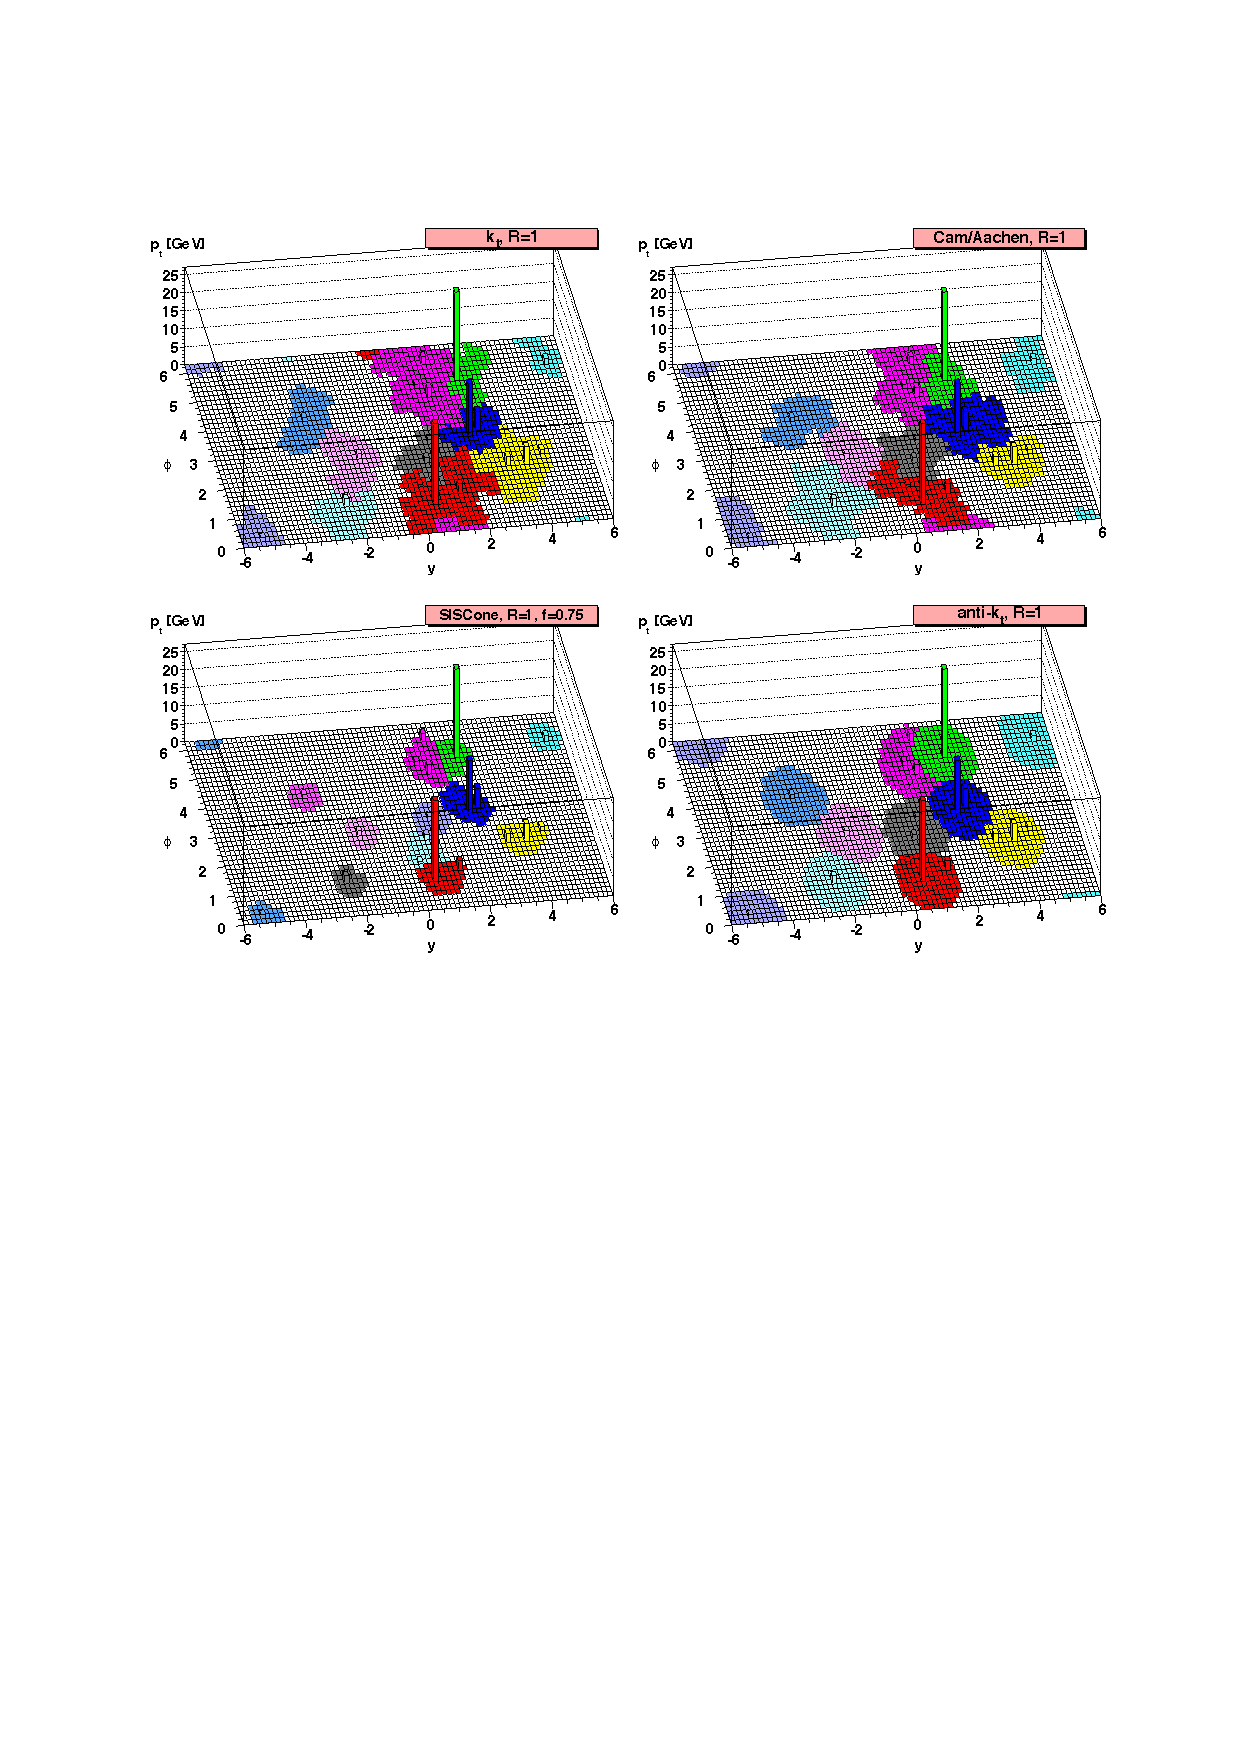
\includegraphics[width=0.9\textwidth]{Figures/diff_algos.pdf}
		%\rule{35em}{0.5pt}
	\caption[Clustering particles into jets with different algorithms.]{Clustering same set of reconstructed particles into jets using different jet algorithms. \cite{Salam:2009jx}}
	\label{fig:jetAlgos}
\end{figure}
\par Parameter $p$ defines which particles are clustered first thus defining the type of algorithm. The $k_T$ algorithm uses $p=1$, clustering soft particles first. This results in irregularly shaped jets, as shown in figure \ref{fig:jetAlgos}, which are sensitive to radiation in the event and difficult to calibrate. The \textit{Cambridge-Aachen} algorithm (CA) uses $p=0$ thus relying only on angular distribution of the input particles. This approach is particularly useful for jet substructure analysis and is less sensitive to radiation. The algorithm used in this analysis is $anti-k_T$ algorithm where $p=-1$ clusterizing the hardest particles first \cite{Cacciari:2008gp}. $Anti-k_T$ is an IRC safe algorithm with jets that are circular in shape because they are not affected by the softer components of the jet.       


%-----------------------------------
%	SUBSECTION 3.2
%-----------------------------------

\subsection{Jet corrections}
\label{sec:jetCorr}

Measured jet energy at detector level in general doesn't correspond to the energy of the originating particle. Jet calibration procedure is introduced to compensate for the nonlinear response of the calorimeters. This is done using a factorized approach where corrections on each level of correction are determined separately as described in \cite{Chatrchyan:2011ds}. Final corrected jet momentum is obtained from measured $p^{raw}$ according to:
\begin{equation}
p^{corr} = C_{offset}(p_T^{raw},\eta)\times C_{rel}(\eta) \times C_{abs}(p'_T) \times C_{res}(p_T'',\eta) \times p^{raw}
\end{equation}     
where offset correction $C_{offset}$ and calibration factors $C_{rel}$ and $C_{abs}$ are applied to both data and simulation, $C_{res}$ is applied only to data. Corrections are applied sequentially, in a fixed order such that $p_T' = C_{offset} \times C_{rel}(\eta) \times p^{raw}$ , and $p_T'' = C_{rel}(\eta) \times C_{abs}(p'_T)$. Correction factors used in this analysis can be found in \cite{CMS-DP-2013-033}.
Each level of corrections is summarized below:
\begin{itemize}
\item Offset correction $C_{offset}$ compensates for energy contributions arising from pile-up events or instrument noise. The offset is determined in dependence of pseudorapidity, jet area $p_T density$ which is described in \cite{Cacciari2008119}.
\item Relative correction $C_{rel}$ is aimed to flattening the jet scale in pseudorapidity. The correction is determined from simulation, adjusting the jet scale in all $\eta$ regions to one of the jets in $|\eta|<1.3$ without changing the absolute scale.
\item Absolute correction $C_{abs}$ flattens the jet scale in $p_T$. This correction is also determined from QCD multijet events as inverse of average response at fixed $p_T^{gen}$.
\item Residual correction $C_{res}$ is applied only to data in order to account for possible residual differences in data and simulation agreement after applying absolute and relative corrections. These corrections are derived using events with momentum balance in transverse plane, like dijet events or $Z/\gamma$ + jet events.
\end{itemize}
The total jet correction for a fixed jet $p_T$ as a function of pseudorapidity is shown in figure \ref{fig:tot_corr_eta}.
\begin{figure}[htbp]
	\centering
		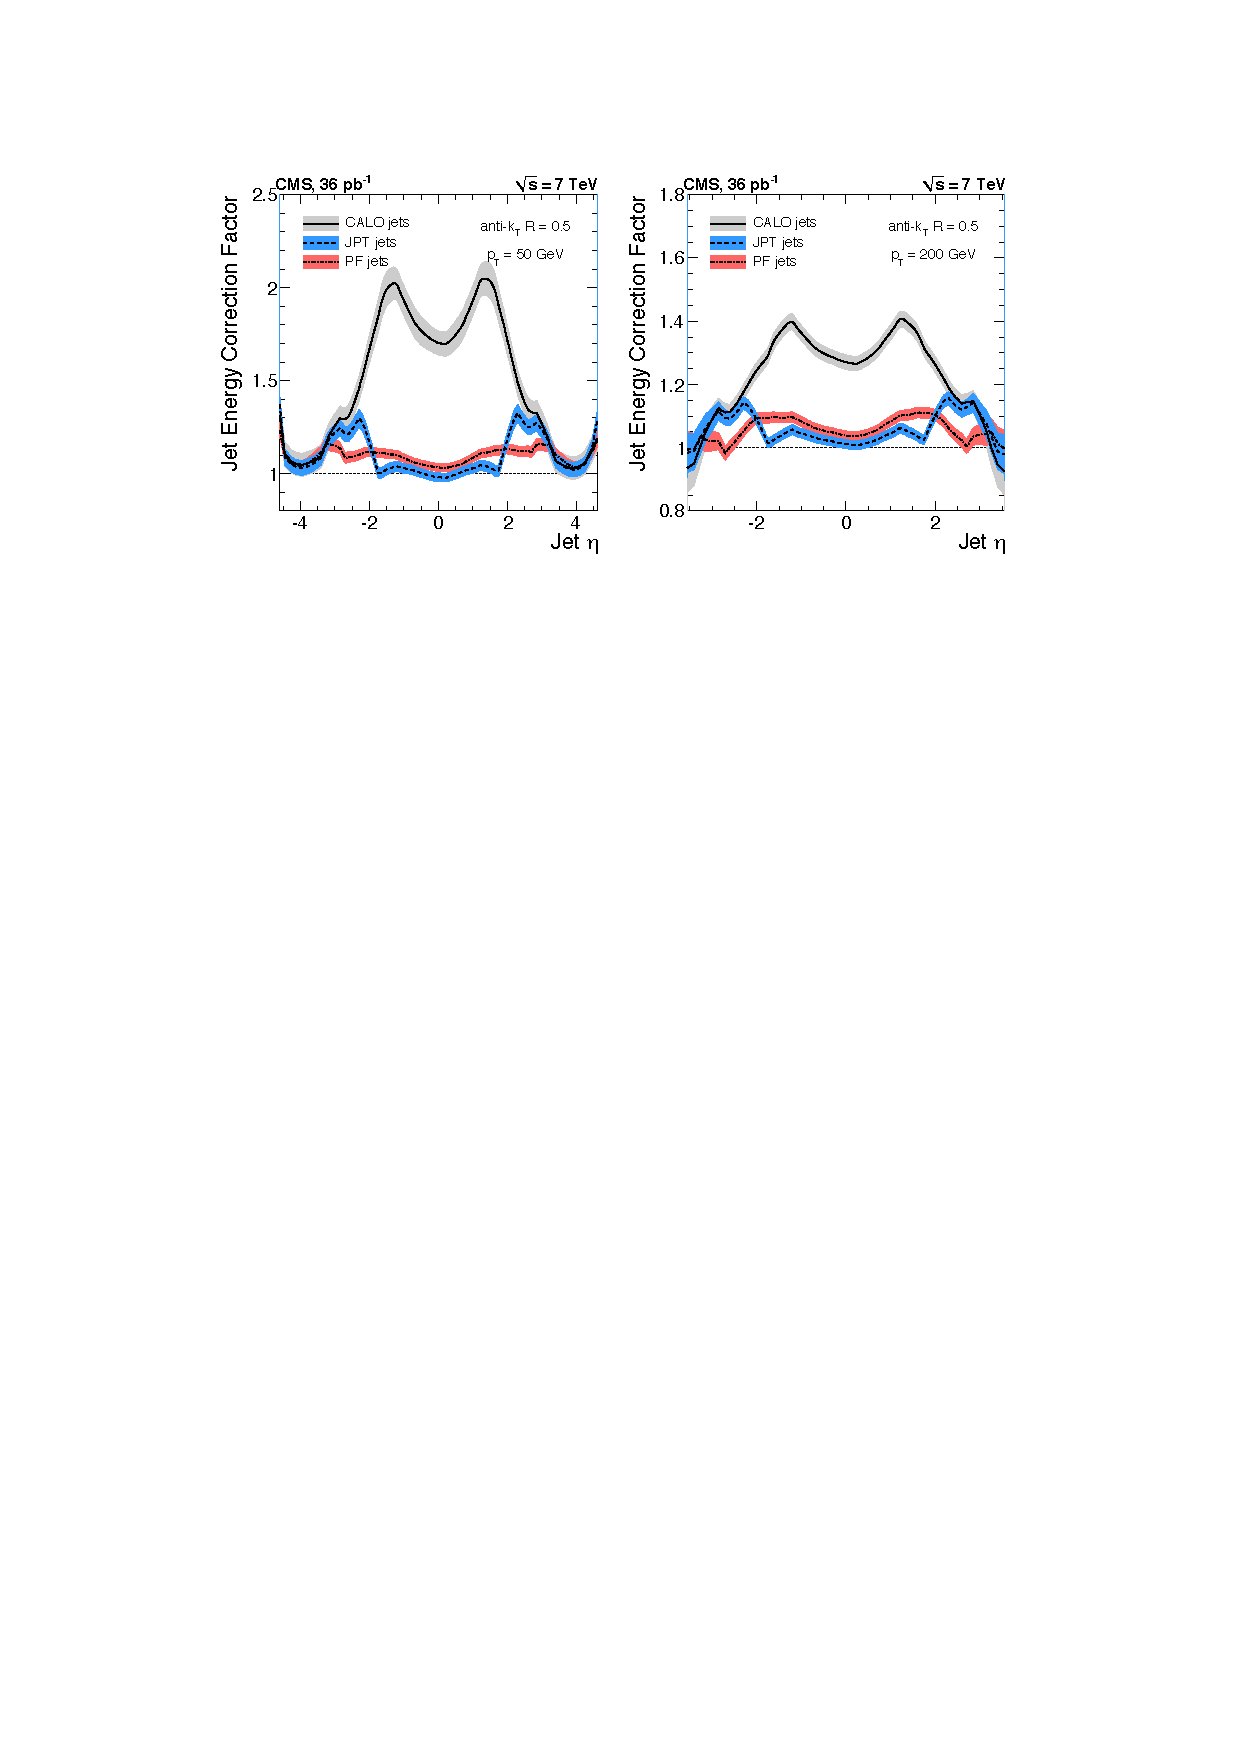
\includegraphics[width=0.9\textwidth]{Figures/jet_tot_corr_eta.pdf}
		%\rule{35em}{0.5pt}
	\caption[Total jet energy correction as a function of pseudorapidity of two different jet $p_T$ values.]{Total jet energy correction as a function of pseudorapidity of two different jet $p_T$ values. Corrections are shown for all three types of jets, calo, JPT and PF jets. Bands indicate corresponding uncertainty.}
	\label{fig:tot_corr_eta}
\end{figure}

\begin{figure}[htbp]
	\centering
		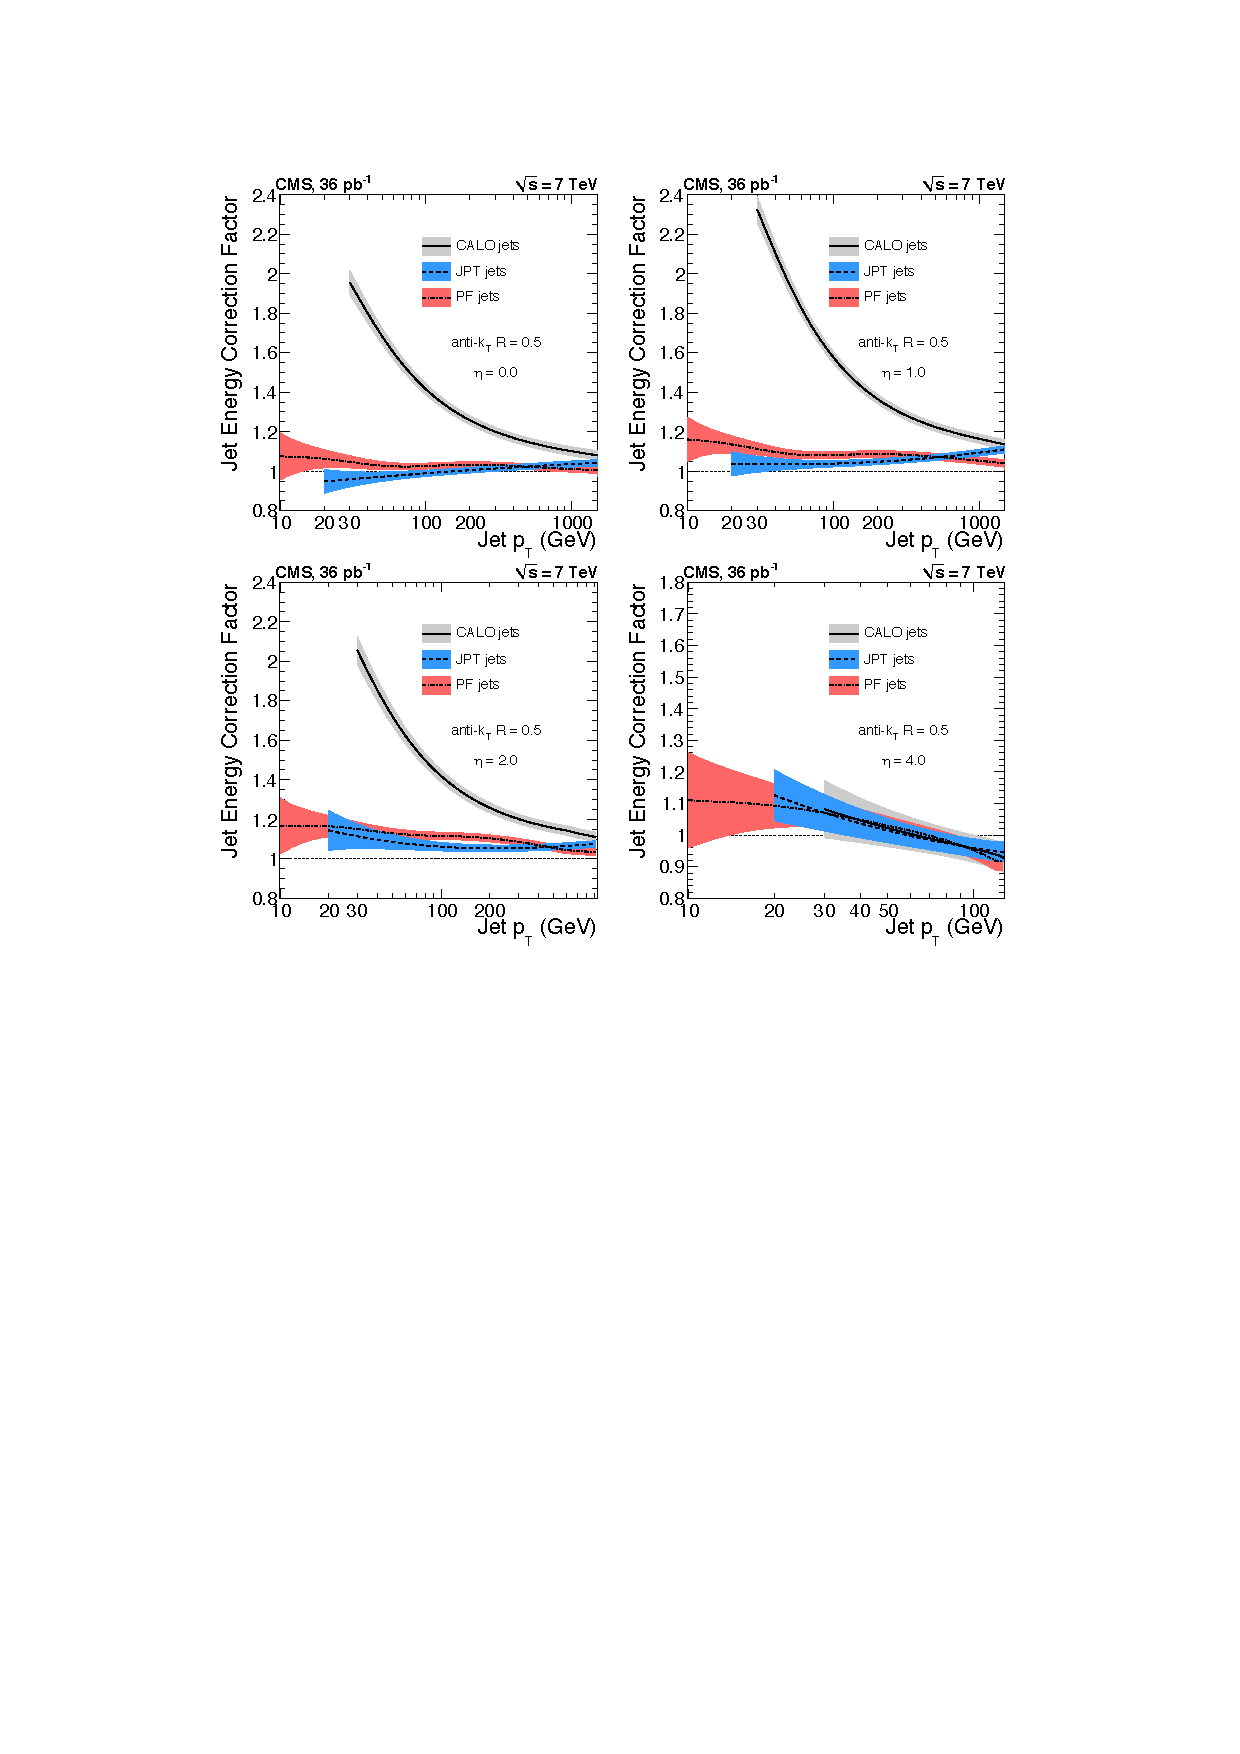
\includegraphics[width=0.9\textwidth]{Figures/jet_tot_corr_pt.pdf}
		%\rule{35em}{0.5pt}
	\caption[Total jet energy correction as a function of transverse momentum for four different $\eta$ values.]{Total jet energy correction as a function of transverse momentum for four different $\eta$ values. Corrections are shown for all three types of jets, calo, JPT and PF jets. Bands indicate corresponding uncertainty.}
	\label{fig:tot_corr_pt}
\end{figure}
%-----------------------------------
%	SUBSECTION 3.3
%-----------------------------------

\subsection{Jet identification}
\label{sec:jetID}
This analysis uses $anti-k_T$ algorithm with cone size $R=0.5$. Jet algorithm implementation is done in the \textit{Fast-jet} package \cite{Cacciari:2011ma}. Depending on which signals is the algorithm applied to, there are different kinds of jets: calo jets (using calorimeter deposits), jet-plus-track jets (calorimeter deposits complemented with tracker information) and most widely used \textit{particle flow} jets (PF). These jets are clustered from PF particles identified with PF algorithm, thus using the information not only from HCAL, but also from tracking system and ECAL which show much better resolution. Only neutral fraction of the jet is measured only with HCAL which makes about 15$\%$ of the total jet composition. PF jets show excellent performance and are the default jets for most CMS analysis. Pile-up information is also taken into account by removing charged hadrons originating from pile-up vertices from the list of particles available for the jet clusterization. This procedure is called \textit{charged hadron subtraction}. Some additional cuts to the jet composition are applied in order to endure good jet identification.  
  \begin{table}[h]
\centering
  \caption{A summary of jet identification criteria.}
  \label{tab:jetID}
  \begin{tabular}{ l  c c}
      \hline
      \hline
      	Variable & Requirement \\
      	\hline
    		Neutral hadron fraction & $<$ 0.99  \\
     	Neutral EM fraction & $<$ 0.99 \\
     	Number of Constituents & $>$ 1 \\		
		\hline
		Additional cuts for $|\eta|<2.4$ \\
		\hline
		Charged hadron fraction & $>$ 0 \\ 
		Charged multiplicity & $>$ 0 \\
		Charged EM fraction & $<$ 0.99 \\
      \hline
      \hline 
  \end{tabular}
\end{table}

%-----------------------------------
%	SUBSECTION 3.4
%-----------------------------------

\subsection{Jets from b quarks}
\label{sec:btagging}

Unique properties of the bottom quark can be used to identify hadronic jets originating from b quarks which are usually referred to as b-jets. Long lifetime of B hadrons is a consequence of weak force decay which results in their displacement by few micrometers at the LHC energies. B hadron decays show a large number of tracks with hard $p_T$ spectrum and soft leptons emerging from semi-leptonic decays. The process of b-jet identification is called $b-tagging$. This process takes one or more variables and produces a single discriminant value for each jet. This value shows how much the observed jet looks like a b-jet. There are several \textit{b-tagging} algorithms in use at CMS which are described in detail in \cite{Chatrchyan:2012jua} and the following were used in 2012 data analysis:
\begin{itemize}
	\item \textit{Track counting}(TC) - The discriminant value is the impact parameter significance which is calculated as impact parameter value divided by the respective impact parameter uncertainty. Impact parameter values are sorted in the decreasing order. Depending on whether second or third value is chosen, the algorithm is denoted as high efficiency or high purity. 
	\item \textit{Jet Probability}(JP) - This algorithm combines information from several tracks inside a jet by computing a likelihood thet all tracks originated from the primary vertex.  
	\item \textit{Combined secondary vertex}(CSV) - This is the most efficient \textit{b-tagging} algorithm currently used at CMS. Both secondary vertex and track related information are combined to build a CSV discriminant value. It shows high efficiency even when no good secondary vertex can be reconstructed. Some of the variables used in CSV algorithm are flight distance, vertex mass, impact parameter significance, track multiplicity at the vertex and track multiplicity in a jet. The distribution of CSV discriminant value is shown in figure \ref{fig:csv}.
\end{itemize}
\begin{figure}[ht]
	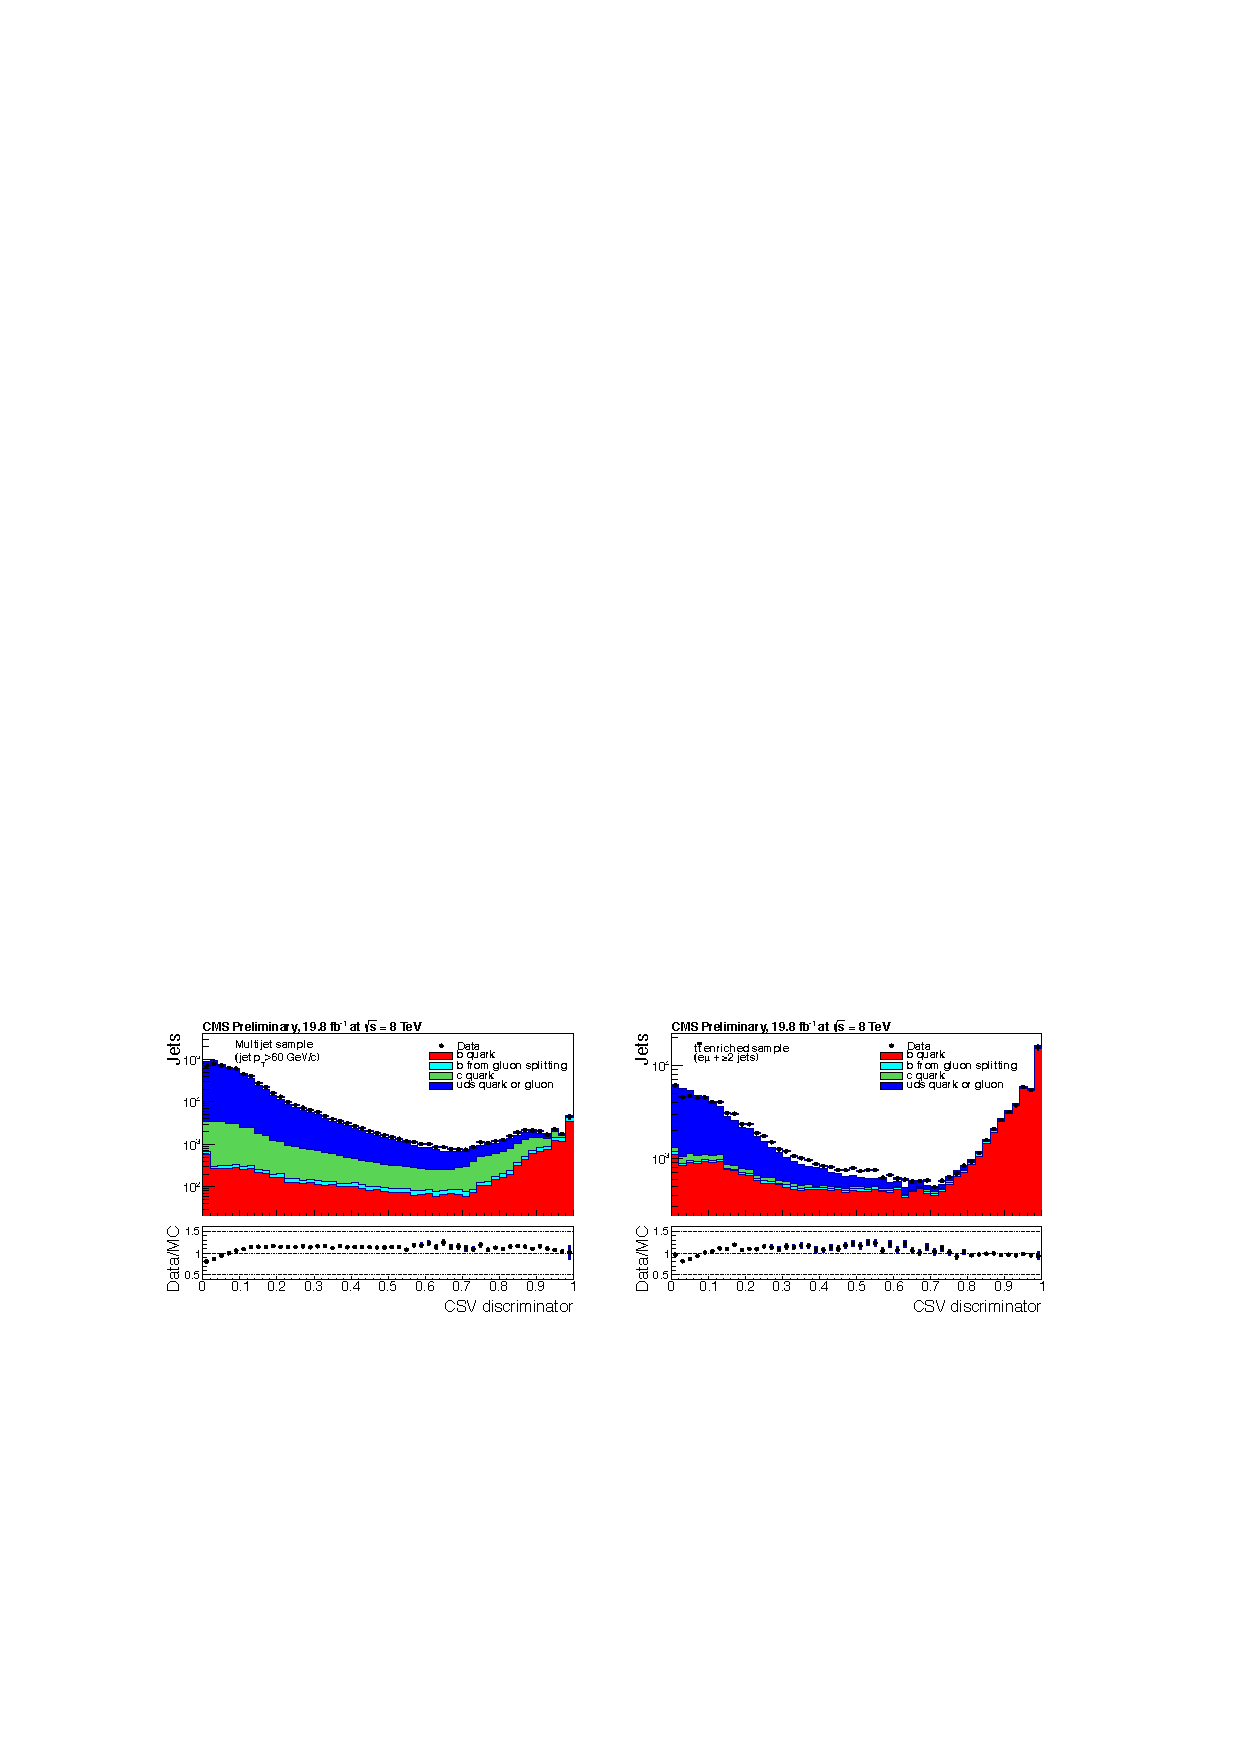
\includegraphics[width=\textwidth]{Figures/b-tag_csv.pdf}
	\caption{Combined secondary vertex discriminant value for multijet QCD sample (left) and tt enriched sample(right)\cite{CMS:2013vea}}
	\label{fig:csv}
\end{figure}
For each non-b-jet there is a chance that it would be identified as b-jet. Based on this misidentification rate, three operating points have been defined for the discriminant value: loose, medium and tight. For an average jet of 80 GeV, these values correspond to misidentification rates of 10\%, 1\% and 0.1\% respectively. Misidentification probabilities as a function of b-jer efficiency for several algorithms are shown in figure \ref{fig:misID}. 
\begin{figure}[ht]
\centering
	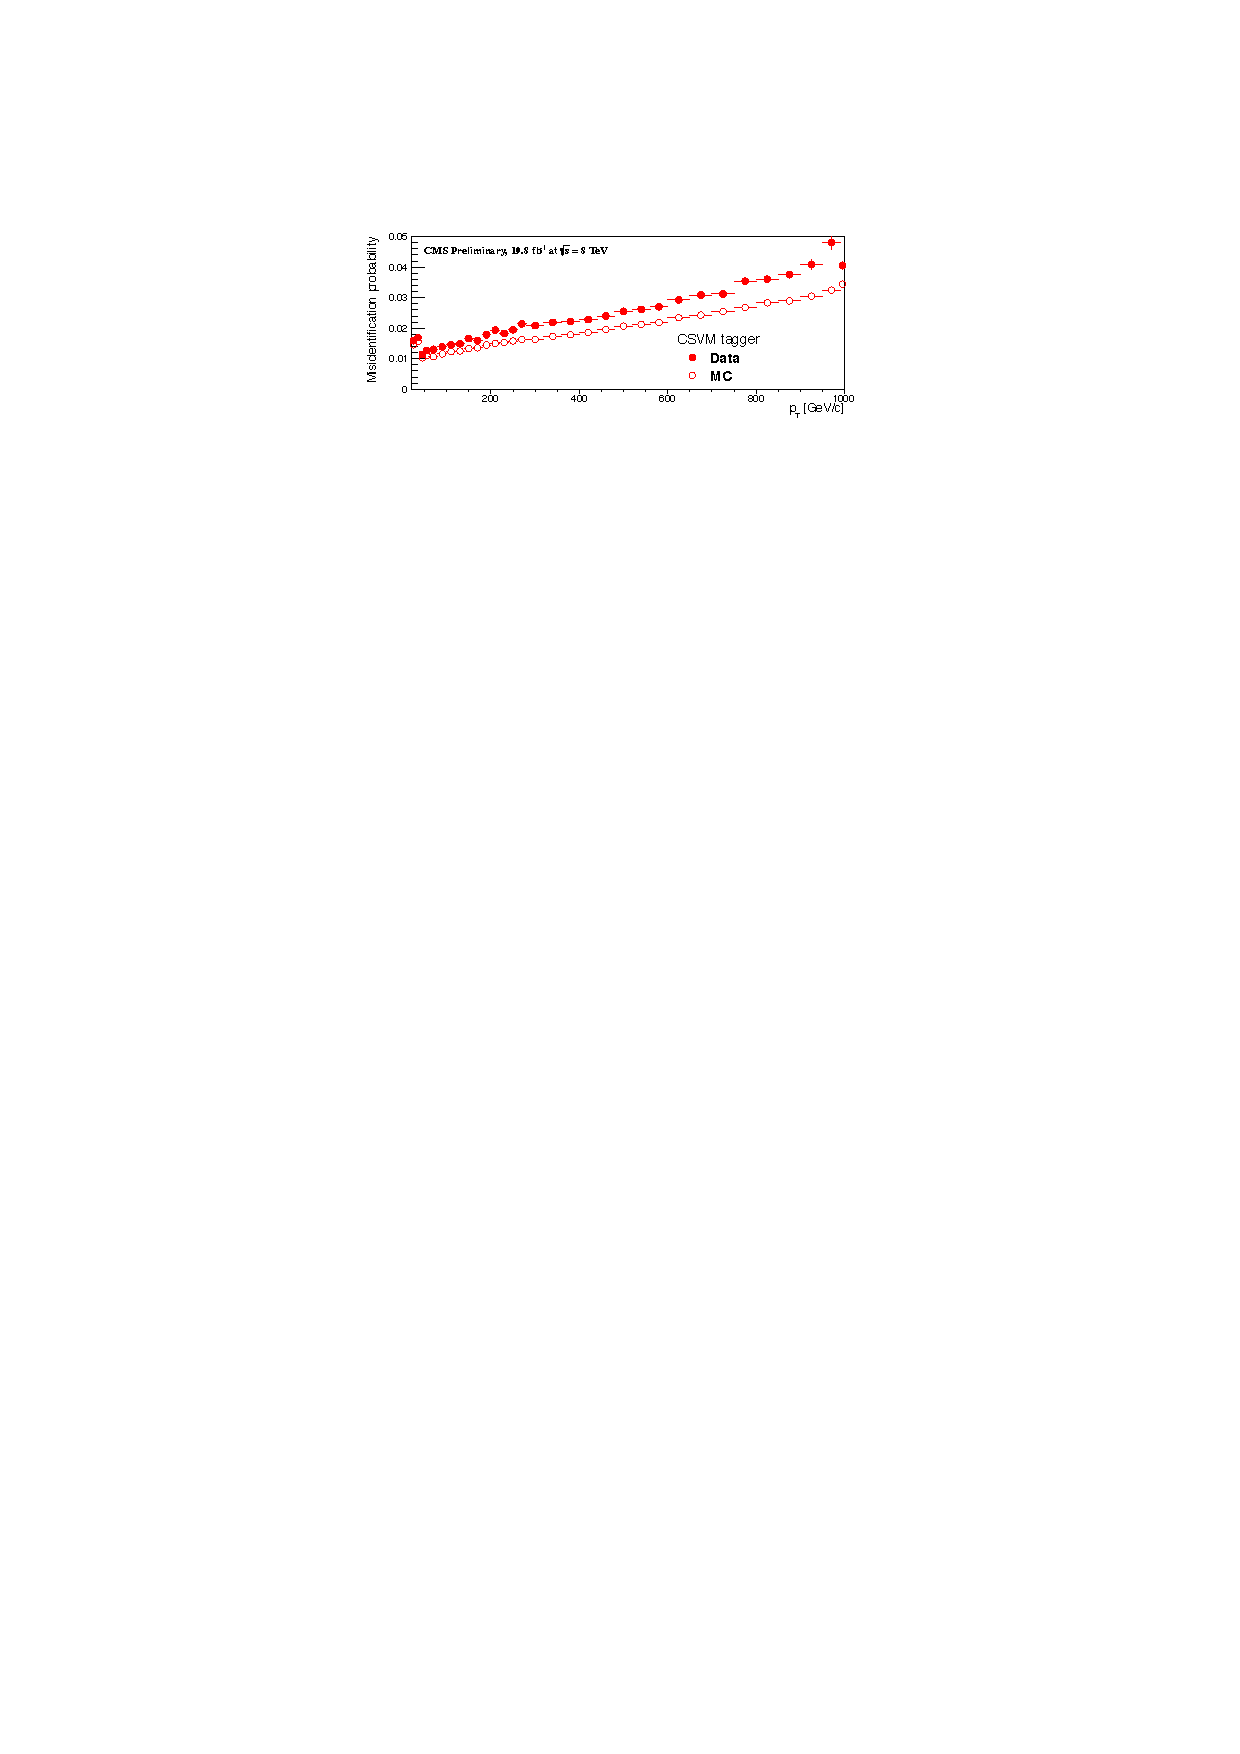
\includegraphics[width=0.6\textwidth]{Figures/MisID_CSVM.pdf}
	\caption{Combined secondary vertex misidentification probability for data and MC for medium working point.\cite{CMS:2013vea}}
	\label{fig:misID}
\end{figure}



%----------------------------------------------------------------------------------------
%	SECTION 4
%----------------------------------------------------------------------------------------

\section{Missing transverse energy}

Missing transverse momentum is the imbalance in the vectorial sum of transverse momenta of all measured particles. Momentum conservation delegates that the imbalance arises from weakly interacting neutral particles such as neutrinos. Missing transverse energy is the magnitude of the missing transverse momentum and is calculated as:
\begin{equation}
E_T^{miss}= |-\sum_{i} \vec{p}_i|
\end{equation}
where $i$ goes over all visible particles. Measurement of the missing transverse energy relies on the good measurement of all other particles in the event and as such is very sensitive to detector inefficiencies, particle missmeasurements, limited acceptance of the detector, cosmic-ray particles all of which can cause artificial missing energy. There are several approaches to determine $E_T^{miss}$. In this analysis, particle flow technique is used which tries to identify each particle in the event by combining the information from all subdetectors and gives the best missing energy resolution.\cite{CMS-PAS-PFT-09-001,Chatrchyan:2011tn} Several corrections are applied to the $E_T^{miss}$ which correct for the possible bias in the missing energy measurement:
\begin{itemize}
\item Type-I correction: propagates jet energy corrections described in Section \ref{sec:jetCorr} to missing energy. This correction replaces the missing energy calculated by summing transverse momenta of particles in a jet by transverse momentum of a jet to which JEC were applied.
\item xy-shift correction: aimed at correcting the observed missing energy $\phi$ modulation. True missing energy distribution is expected not to depend not to depend of $\phi$ because of the rotational symmetry of collisions around the beam axis. The possible cause for such modulation  include unisotropic detector response, detector misalignment, the displacement of the beam spot. The amplitude of the modulation is observed to increase with the number of pile-up interactions so this correction can be seen as mitigation for the pile-up effects.
\end{itemize}




 
% Chapter Template

\chapter{Event selection and analysis strategy} % Main chapter title

\label{Chapter6} % Change X to a consecutive number; for referencing this chapter elsewhere, use \ref{ChapterX}

\lhead{Chapter 6. \emph{Event selection and analysis strategy}} % Change X to a consecutive number; this is for the header on each page - perhaps a shortened title

%----------------------------------------------------------------------------------------
%	SECTION 1
%----------------------------------------------------------------------------------------

\section{Analysis strategy}


%-----------------------------------
%	SUBSECTION 1
%-----------------------------------
\subsection{Subsection 1}



%-----------------------------------
%	SUBSECTION 2
%-----------------------------------

\subsection{Subsection 2}


%----------------------------------------------------------------------------------------
%	SECTION 2
%----------------------------------------------------------------------------------------

\section{Background estimation}

 
% Chapter Template

\chapter{Prosireni sazetak:} % Main chapter title

\label{Chapter7} % Change X to a consecutive number; for referencing this chapter elsewhere, use \ref{ChapterX}

\lhead{Chapter X. \emph{Chapter Title Here}} % Change X to a consecutive number; this is for the header on each page - perhaps a shortened title

%----------------------------------------------------------------------------------------
%	SECTION 1
%----------------------------------------------------------------------------------------

\section{Main Section 1}

Lorem ipsum dolor sit amet, consectetur adipiscing elit. Aliquam ultricies lacinia euismod. Nam tempus risus in dolor rhoncus in interdum enim tincidunt. Donec vel nunc neque. In condimentum ullamcorper quam non consequat. Fusce sagittis tempor feugiat. Fusce magna erat, molestie eu convallis ut, tempus sed arcu. Quisque molestie, ante a tincidunt ullamcorper, sapien enim dignissim lacus, in semper nibh erat lobortis purus. Integer dapibus ligula ac risus convallis pellentesque.

%-----------------------------------
%	SUBSECTION 1
%-----------------------------------
\subsection{Subsection 1}

Nunc posuere quam at lectus tristique eu ultrices augue venenatis. Vestibulum ante ipsum primis in faucibus orci luctus et ultrices posuere cubilia Curae; Aliquam erat volutpat. Vivamus sodales tortor eget quam adipiscing in vulputate ante ullamcorper. Sed eros ante, lacinia et sollicitudin et, aliquam sit amet augue. In hac habitasse platea dictumst.

%-----------------------------------
%	SUBSECTION 2
%-----------------------------------

\subsection{Subsection 2}
Morbi rutrum odio eget arcu adipiscing sodales. Aenean et purus a est pulvinar pellentesque. Cras in elit neque, quis varius elit. Phasellus fringilla, nibh eu tempus venenatis, dolor elit posuere quam, quis adipiscing urna leo nec orci. Sed nec nulla auctor odio aliquet consequat. Ut nec nulla in ante ullamcorper aliquam at sed dolor. Phasellus fermentum magna in augue gravida cursus. Cras sed pretium lorem. Pellentesque eget ornare odio. Proin accumsan, massa viverra cursus pharetra, ipsum nisi lobortis velit, a malesuada dolor lorem eu neque.

%----------------------------------------------------------------------------------------
%	SECTION 2
%----------------------------------------------------------------------------------------

\section{Main Section 2}

Sed ullamcorper quam eu nisl interdum at interdum enim egestas. Aliquam placerat justo sed lectus lobortis ut porta nisl porttitor. Vestibulum mi dolor, lacinia molestie gravida at, tempus vitae ligula. Donec eget quam sapien, in viverra eros. Donec pellentesque justo a massa fringilla non vestibulum metus vestibulum. Vestibulum in orci quis felis tempor lacinia. Vivamus ornare ultrices facilisis. Ut hendrerit volutpat vulputate. Morbi condimentum venenatis augue, id porta ipsum vulputate in. Curabitur luctus tempus justo. Vestibulum risus lectus, adipiscing nec condimentum quis, condimentum nec nisl. Aliquam dictum sagittis velit sed iaculis. Morbi tristique augue sit amet nulla pulvinar id facilisis ligula mollis. Nam elit libero, tincidunt ut aliquam at, molestie in quam. Aenean rhoncus vehicula hendrerit. 
% Chapter Template

\chapter{Conclusions} % Main chapter title

\label{Chapter8} % Change X to a consecutive number; for referencing this chapter elsewhere, use \ref{ChapterX}

\lhead{Chapter 8. \emph{Conclusions}} 

% sto je prezentirano i zasto
This thesis presents the inclusive cross section measurement for W boson production in association with two b jets in proton-proton collisions at $\sqrt{s}=$8 TeV. The analyzed data is collected with the CMS detector during 2012, corresponding to the integrated luminosity of 19.8 fb$^{-1}$. From the theoretical point of view, this process is important as a probe into the perturbative QCD calculations and can lead to improvement of theoretical calculations. On the other hand, from the experimental  point of view of an experimentalist, accurate  knowledge of Wbb process leads to more precise measurements of other processes to which this one is a background, such as the top quark or associated Higgs and W boson production, with Higgs boson  decaying to a pair of b quarks.

% koji su rezultati
\par The cross section measurement was performed in the fiducial region defined by a presence of a lepton and exactly two 2 b-tagged jets. The result is quoted separately in muon and electron channel. The measured values in the two channels are compatible, as predicted by the standard model. The theoretical cross section was derived using MCFM and was compared to the measured values. The measured values are around one standard deviation higher than the predicted theoretical values. Several measurements including a W boson and b jets in the final state were performed in the past, however the results cannot be directly compared because of different phase space and slightly different final states.

% kako popraviti rezultate
The uncertainty on the measured values is dominated by the systematic effects. The largest uncertainties are associated with the b tagging procedure and jet related uncertainties, jet energy scale and jet energy resolution. Reducing these uncertainties in the future, would allow for sensitive test of perturbative QCD calculation at next-to-leading order level.

% sto ce se dogadjati u buducnosti
After the long shutdown, which started in 2013, LHC has just restarted its operations, reaching the highest energy of $\sqrt{s}=$ 13 TeV. This marks the start of another exciting period, which is aimed at Higgs boson precision measurements, supersymmetry and dark matter searches. As for the measurements of W boson produced in association with b quarks, one of the main goals for the future is reducing the large systematic uncertainties as stated previously. Measuring differential cross section as a function of various variables, like leading jet transverse momentum, would be of great interest to theorists. Another goal would be to probe different final states, for example studying events with two B hadrons in the same jet, or using track based tagging without requiring jets. This would allow us to study collinear final state in depth.


% Chapter Template

\chapter{Strukturirani sažetak - Mjerenje udarnog presjeka zajedničke produkcije W bozona i para b kvarkova} % Main chapter title

\label{Chapter9} % Change X to a consecutive number; for referencing this chapter elsewhere, use \ref{ChapterX}

\fancyhead[LE,RO]{Chapter 9. \emph{Strukturirani sažetak}} % Change X to a consecutive number; this is for the header on each page - perhaps a shortened title
\begin{otherlanguage}{croatian}
%----------------------------------------------------------------------------------------
%	SECTION 1
%----------------------------------------------------------------------------------------

\section{Uvod}
Standardni model fizike elementarnih čestica je teorija nastala šezdesetih i sedamdesetih godina dvadesetog stoljeća, pokušavajući odgovoriti na pitanje od čega je materija načinjena i kako interagira. Predviđanja Standardnog modela testirana su veliki put puta različitim eksperimentima, međutim nikada nisu opovrgnuta. Jedina nedostajuća karika bio je Higgsov bozon, čestica čije je postojanje portvrđeno 2012. godine, a svojstva su joj izmjerena narednih godina. Time je zaokružena slika Standardnog modela. Međutim, postoje različiti fenomeni koji ne se ne mogu opisati u okviru Standardnog modela kao što su postojanje neutrinskih oscilacija, asimetrije između materija i antimaterije, postojanje tamne materije i tamne energije. Ovi fenomeni upućuju na postojanje fizike izvan Standardnog modela. Osjetljivost pojedinog eksperimenta na opažanje takvih fenomena izravno je povezano s preciznim mjerenjem već postojećih procesa. 

Događaji u kojima je W bozon produciran zajedno s b kvarkvima u središtu je različitih teorijskih i eksperimentalnih istraživanja. Međutim, teorijska predviđanja još uvijek ne objašnjavaju dovoljno dobro  eksperimentalne rezultate zbog pojave divergencija u slučaju kada izračeni gluoni imaju jako malu energiju ili je par kvarkova kolinearan. Nadalje, precizno mjerenje W bozona produciranog s parom b kvarkova omogućava bolje razumijevanje i teorijska predviđanja u okviru perturbativne kvantne kromodinamike (pQCD) i provjere valjanosti različitih teorijskih modela korištenih u simulacijama. Ovaj proces je i pozadina za različita mjerenja u okviru Standardnog modela, uključujući mjerenja povezana s top kvarkom i Higgsovim bozonom koji se raspada u par b kvarkova. 

Tema ove teze je mjerenje udarnog presjeka za proces $pp\rightarrow W+bb+X$ koristeći podatke prikupljene CMS detektorom tijekom 2012 godine na energiji $\sqrt{s} = 8$ TeV. W bozon se raspada na elektron ili mion i odgovarajući neutrino. Prisutnost W bozona se očituje kroz postojanje izoliranog leptona visokog impulsa te nedostajuće energije koja dolazi od slabo interagirajućeg neutrina. Kvarkovi se u detektoru vide kao usmjereni mlazovi čestica te prolaze kroz posebne algoritme koji identificiraju mlazove nastale od b kvarkova.

\section{Teorijski uvod i prethodna mjerenja}

Složenost sudara protona proizlazi iz njihove unutarnje strukture. Iako je proton najvećim dijelom sastavljen od $uud$ valentnih kvarkova, ostali kvakovi koje nazivamo kvarkovima mora, te gluoni također mogu sudjelovati u sudarima. Točna predviđanja konačnih stanja u sudarima protona uvelike ovise o kombinaciji teorijskih izračuna i eksperimentalnih rezultata. Opis takvih konačnih stanja se dijeli u nekoliko stupnjeva koji se odvijaju na različitim energijskim skalama. Na najvišim energijama se odvija tvrdi proces koji rezultira produkcijom teških ili visoko-energetskih čestica. Teške čestice se potom raspadaju na lakše. Ova dva procesa opisuju se matrični elementom. Pljusak partona je idući stupanj u opisu sudara protona i označava proces u kojem su izračene lagane čestice, fotoni i gluoni, koji su često kolinearni s originalnom česticom. Zadnji stupanj je hadronizacija tijekom koje partoni formiraju hadrone čijim se raspadima produciraju stabilne čestice opažene u detektoru.
\par Prethodna mjerenja procesa koji u konačnom stanju sadrže W bozon i b kvarkove izvršena su na Tevatronu, eksperimentima CDF i D0 \cite{Aaltonen:2009qi,D0:2012qt} te na LHC-u, eksperimentima ATLAS i CMS \cite{Aad:2013vka,Chatrchyan:2013uza}. Prethodna mjerenja ne mogu se izravno uspoređivati, budući da su proučavana različita konačna stanja u različitim faznim prostorima. Međutim, usporedba sa teorijskim predviđanjima ukazuje na slaganje. 

\section{LHC}
Veliki hadronski sudarivač je ubrzivač protona smješten na švicarsko-francuskoj granici, u blizini Ženeve \cite{Evans:2008zzb}. Nalazi se u podzemnom tunelu promjera 27 km, na prosječnoj dubini od 100 m. Veliki hadnonski sudarivač je najveći u nizu akceleratora čija je zadaća postupno ubrzavanje čestica, do maksimalne energije $\sqrt{s}=$ 14 TeV. Snopovi čestica, kada dosegnu ciljanu energiju, sudaraju se na četiri mjesta gdje su izgrađeni detektori koji mjere čestice nastale u sudarima. Na dva mjesta nalaze se detektori široke namjene ATLAS (A Toroidal LHC Apparatus) \cite{Aad:2008zzm} i CMS (Compact Muon Solenoid) \cite{Chatrchyan:2008aa}.  Ovi detektori pokrivaju široki spektar tema iz fizike visokih energija, uključujući potragu za Higgsovim bozonom, supersimetričnim česticama, te detaljna mjerenja svojstava Standardnog modela. ALICE (A Large Ion Collider Experiment) detektor proučava kvarkovsko-gluonsku plazmu u sudarima iona olova \cite{Aamodt:2008zz}. LHCb (LHC Beauty) je usmjeren na pručavanje B fizike kroz raspade B mezona \cite{Alves:2008zz}. LHC je modularni ubrzivač sastavljen od oko 10000 različitih supravodljivih magneta koji fokusiraju i usmjeravaju snop čestica.
\par Snopovi se ubrizgavaju u LHC u obliku paketa protona te se ubrzavaju pomoću radiofrekventnih komora (RF). Tijekom 2012. godine, prosječan broj sudara je bio oko 21 unutar jednog sudara paketa protona. Broj sudara po jedinici vremena se naziva luminozitet, a ukupan broj sudara se u nekom vremenskom periodu se naziva integrirani luminozitet. Tijekom 2012. godine ukupno je prikupljeno više od 24 fb$^{-1}$ inegriranog luminoziteta. 

 
\section{CMS detektor}
Kompaktni mionski solenoid (CMS) izgrađen je oko jedne od četiri točaka interakcije na velikom hadronskom sudarivaču. Detektor je slojevitog cilindričnog dizajna, hermetički zatvoren i gotovo potpuno pokriva cijeli prostorni kut oko točke interakcije. CMS detektor koristi desni koordinatni sustav s ishodištem u središtu detektora. $z$ os je postavljena duž smjera snopa, $x$ os je usmjerena prema središtu prstena, a $y$ os je okomita na njih. Detektor je podijeljen na centralni dio ($barrel$) koji se proteže do $\eta \approx \pm 1.5$, te bočne dijelove ($endcaps$). Unutar CMS-a nalazi se solenoid koji generira polje od 3.8 T u unutarnjem volumenu i oko 2 T izvan.  Unutar solenoida nalaze se detektor tragova i kalorimetri, a izvan mionske komore. Jako magnetsko polje zakreće putanje nabijenih čestica nastalih u sudarima i omogučava mjerenje njihovog impulsa. 
\par U samom središtu detektora, oko točke interakcije, smješten je silicijski piksel detektor. Sastoji se od tri sloja u središnjem dijelu i dva diska sa svake strane i sadrži oko 66 milijuna piksela. Oko njega nalazi se silicijski $strip$ detektor, koji se sastoji od niza žica. U žicama se prolaskom nabijene čestice inducira naboj koji se potom dovodi do silicijskih detektora. 
\par Elektromagnetski kalorimetar (ECAL) izgrađen je od olovnog volframata, kristala velike gustoće i malog Moliereovog radijusa, što rezultira kratkim i uskim pljuskovima prilikom upada fotona ili elektrona. Hadronski kalorimetar (HCAL) sastoji se od slojeva mjedenih absorbera i plastičnih scintilatora u središnjem dijelu, te čeličnih absorbera i kvarcnih scintilatora u bočnim dijelovima. Svrha hadronskog kalorimetra je zastavljanje hadronskih snopova, što se događa u absorberima, a rezultirajući pljusak čestica se detektira scintilatorima. 
\par Mionske komore sastoje se od nekoliko vrsta detektora punjenih plinom. Driftne komore smještene su u središnjem dijelu i napunjene su plinom koji se ionizira prolaskom čestice. Katodne trakaste komore nalaze se u bočnim dijelovima te funkcioniraju na isti način kao i driftne komore, ali su dodatno isprepletene velikim brojem žica za prikupljanje naboja. Komore s otpornim pločama sastoje se od paralelnih ploča velike otpornosti između kojih je plin. U slučaju prolaska čestice dolazi do ionizacije plina i stvaranja pljuska elektrona. Ove detektore karakterizira visoka vremenska razlučivost, te su pogodni za korištenje kao dio sustava za okidanje. 
\par Protoni u LHC-u se sudaraju frekvencijom od 40 MHz i generaju veliku količinu podataka koju nije moguće pohraniti. Uzimajući u obzir da su udarni presjeci za zanimljive fizikalne procese redove veličina manji od udarnog presjeka za sudar protona, potrebno je konstruirati sustav okidača koji će zapisivati samo zanimljive događaje. Ovaj sustav je dizajniran na dvije razine. Prva razina koristi posebnu elektroniku i pomoću jednostavnih zahtjeva na svaki događaj, uspijeva unutar 3 $\mu$s smanjiti broj događaja s 40 MHz na oko 100 kHz. Iduća razina se naziva \textit{High Level Trigger} (HLT), čija je zadaća smanjiti broj sudara na oko 100 u sekundi.       

\section{Rekonstrukcija fizikalnih objekata}
\par Elektoni u detektoru ostavljaju trag u detektoru tragova i deponiraju energiju u elektromagnetskom kalorimetru. Elektron prolaskom kroz materijal može emitirati i tzv. zakočno zračenje, odnosno fotone koji također deponiraju energiju u elektromagnetskom kalorimetru. Svi energetski depoziti od jednog elektrona formiraju tzv. $supercluster$ koji se potom kombinira s tragom u detektoru tragova koristeći GSM (\textit{Gaussian Sum Filter}) algoritam \cite{CMS:2010bta,2005JPhG31N9A}.
\par Mione karakterizira trag u detektoru tragova i signali u mionskim komorama. Rekonstrukcija kreće od mionskih komora gdje se prilagodbama iz signala rekonstruira trag (tzv. \textit{stanalone muon}). Zatim se izgrađuje globalni mion kombiniranjem traga iz detektora tragova i traga iz mionskih komora \cite{2012JInst7P0002T,Fruhwirth1987444}.   
\par Mlazovi su usmjerena grupa hadrona koja nastaje kao rezultat fragmentacije i hadronizacije kvarkova. Detektirani hadroni se kombiniraju u mlaz posebnim algoritmima, čime se pokušavaju saznati informacije o početnom partonu. Najpopularniji takav algoritam je anti$-k_T$ algoritam koji na osnovu udaljenosti čestica i njihovih impulsa grupira čestice unutar unaprijed definiranog konusa oko čestice najvišeg impulsa \cite{Cacciari:2008gp}. Proces je iterativan i nastavlja se sve dok svi hadroni ne budu pridruženi nekom mlazu. 
\par Mlazovi iz b kvarkova se identificiraju pomoću posebnih algoritama \cite{Chatrchyan:2012jua}. Ti algoritmi koriste karakteristična svojstva b kvarkova kao što su njihova masa i dugo vrijeme života za formiranje jedinstvene varijable koja definira koliko je neki mlaz nalik na mlaz nastao iz b kvarka. Algoritam korišten u ovoj tezi je CSV (\textit{Combined secondary vertex}) koji traga za sekundarnim točkama interakcije koje su odmaknute od mjesta sudara i gleda tragove čestica iz tog mjesta sudara.
\par Nedostajuća transverzalna energija je neravnoteža u transverzalnom impulsu svih detektiranih čestica i određuje se kao:
\begin{equation}
E_T^{miss}= |-\sum_{i} \vec{p}_i|.
\end{equation}
Budući da je trasverzalni impuls očuvan, nedostajuća energija mjeri impuls kojeg odnose nevidljive čestice. Određivanje nedostajuće energije je ovisno o rezoluciji detektora, ograničenoj pokrivenosti prostornog kuta, pogrešnom interpretacijom detektiranog signala ili kozmičkim zrakama. Ove pojave mogu umjetno povećati iznos nedostajuće energije što treba uzeti u obzir \cite{Chatrchyan:2011tn}.  

\section{Selekcija događaja i navažnije pozadine}
 
U tezi su predstavljeni rezultati mjerenja udarnog presjeka za produkciju W bozona zajedno s parom mlazova nastalih iz b kvarka u sudarima protona na energiji $\sqrt{s}=$ 8 TeV. Podaci su prikupljeni 2012. godine CMS detektorom i odgovaraju integriranom luminozitetu od 19.8 fb$^{-1}$. Za simuliranje signala i pozadine korišteni su generatori Madgraph \cite{Alwall:2011uj}, Powheg \cite{Oleari:2010nx} i Pythia \cite{Sjostrand:2006za}. 
\par Zbog boljeg slaganja podataka i simulacija, na simulacije se primjenjuje niz korekcija:
\begin{itemize}
\item Korekcije zbog različitog broja primarnih interakcija. Budući da su simulirani uzorci često generirani prije nego što su uvjeti tijekom prikupljanja podataka poznati, kao što je trenutni luminozitet, potrebno je korigirati simulirane događaje. Korekcija se provodi pridavanjem težine svakom simuliranom događaju tako da raspodjela broja primarnih interakcija u događaju izgleda jednako u podacima i simulacijama \cite{CMS:2013wea}.
\item Efikasnost identifikacije, izolacije i okidača za leptone. Efikasnosti su određene iz podataka korištenjem tzv. \textit{Tag-and-probe} metode, ovisne su o transverzalnom impulsu i pseudorapiditetu te se primjenjuju kao težine za svaki simulirani događaj.
\item Efikasnost algoritma za određivanje b mlazova. Budući da je teško točno modelirati sve parametre koji ulaze u algoritam za određivanje b mlazova, potrebno je korigirati simulirane događaje za omjer efikasnosti algoritma u podacima i simulacijama \cite{CMS:2013vea}.
\end{itemize}
\par Događaji korišteni za mjerenje udarnog presjeka moraju sadržavati W bozon koji se raspada na mion ili elektron, te značajnu količinu nedostajuće energije koja ukazuje na postojanje neutrina. Rekonstruirani mlazovi čestica trebaju zadovoljavati kriterije za b mlazove. Svi kriteriji za selekciju događaja sabrani su ovdje:
\begin{itemize}
\item Jedan mion ili elektron s $p_T>$ 30 GeV i $|\eta|<$2.1  i izolacijskom varijablom $I_{rel}^{PF}<0.12\ (0.10)$ za mione (elektrone),
\item Točno dva mlaza s $p_T>$ 25 GeV i $|\eta|<$2.4 i konusom između mlaza i leptona većim od 0.5,
\item Događaji koji sadrže više od dva mlaza s $p_T>$ 25 GeV i $|\eta|<$2.4 su odbačeni,
\item Događaji koji sadrže dodatni lepton s $p_T>$ 10 GeV i $|\eta|<$2.1 su odbačeni,
\item Oba mlaza moraju imati disktiminantu za određivanje b-mlazova veću od 0.898,
\item Iznos transverzalne mase mora biti veći od 45 GeV.
\end{itemize}  

Najvažnije pozadine uključuju procese s t kvarkovima, Z i W bozone producirane zajedno s mlazovima, dvobozonske događaje te QCD događaje. Pozadine s t kvarkovima su reducirane zahtjevima za točno jednim leptonom i dva mlaza, međutim nakon toga zahjeva, doprinos od tih procesa u konačnom uzorku je oko 60$\%$. Zbog toga je konstruirano posebno kontrolno područje dominirano doprinosom procesa s t kvarkovima u konačnom stanju s ciljem provjere normalizacije tih procesa. Kontrolno područje je dobiveno zahtjevom za više od dva mlaza u konačnom stanju. Uočeno je da je razlika između podataka i simulacija oko 12$\%$ što je uzeto u obzit prilikom određivanja broja događaja signala. 
\par Događaji koji sadrže Z bozon i mlazove u konačnom stanju mogu proći selekciju ako jedan lepton nije dobro rekonstruiran, čime se umjetno stvara nedostajuća energija. Procesi s W bozonom i mlazovima nastalim od lakih kvarkova u konačnom stanju reducirani su na zanemarive vrijednosti postavljanjem zahtjeva na diskriminatornu varijablu b tagging algoritma. Dvobozonski procesi u kojima nastaju W i Z bozon koji se potom raspada na par b kvarkova čine ireducibilnu pozadinu. QCD procesi u konačnom stanju sadrže lepton koji uspjeva proći konačnu selekciju, ali nije nastao raspadom W bozona. Ova pozadina se određuje direktno iz podataka. Oblik raspodjele je određen invertiranjem izolacije na lepton i oduzimanjem MC doprinosa od podataka. Normalizacija raspodjele određuje se u području niskih vrijednosti transverzne mase $M_T<$ 30 GeV.

\section{Rezultati}

Udarni presjek za proces pp$\rightarrow$W+bb+$X$ mjeren je odvojeno u elektronskom i mionskom kanalu i određen je izrazom:
\begin{equation}
\sigma = \frac{N_{sig}}{A\times \epsilon \cdot \mathcal{L}}
\label{equ:xsec_hr}
\end{equation}
gdje je $N_{sig}$ ukupni broj događaja signala koji je određen prilagodbom. $A\times \epsilon$ definira aktivno područje i efikasnost detektora, a $\mathcal{L}$ integrirani luminozitet. 
Aktivno područje i efikasnost detektora definirano je kao:
\begin{equation}
A\times \epsilon=\frac{\mathrm{broj\ izabranih\ Wbb\ događaja}}{\mathrm{broj\ generiranih\ Wbb\ događaja}}
\end{equation}
Ova se vrijednost određuje iz simulacija za svaki kanal posebno. Rezultat je naveden u tablici \ref{tab:AE_hr}.
\begin{table}[!htb]
\begin{center}
   \begin{tabular} {r c} \hline \hline
        Channel         & A$\times \epsilon$ \\
        \hline
        Mionski kanal         & 9.14 $\pm$ 0.18 $\%$ \\
        Elektronski kanal     & 7.66 $\pm$ 0.17 $\%$ \\
        \hline\hline
   \end{tabular}
\caption{Rezultati određivanja A$\times \epsilon$ za mionski i elektronski kanal.}
\label{tab:AE_hr}
\end{center}
\end{table}
Broj događaja signala određen je prilagodbom distribucije transverzne mase koristeći metodu najveće vjerodostojnosti (\textit{maximum likelihood fit}). Prilagodba je izvedena istovremeno u signalnom području i u prethodno opisanom kontrolnom području koristeći distribucije prikazane na slici \ref{fig:mt_hr}. Sistematski efekti su također uzeti u obzir na način da su za svaki doprinos i za svaku pozadinu producirane dvije dodatne distribucijem koje odgovaraju pomaku od jedne standardne devijacije gore i dolje u odnosu na nominalnu vrijednost. Promatrani izvori sistematskih neodređenosti su:
\begin{itemize}
\item Mjerenje energije mlazova,
\item Rezulucija mlazova,
\item Efikasnost određivanja b mlazova,
\item Mjerenje energije leptona,
\item Efikasnost okidača te identifikacije i izolacije leptona,
\item Nedostajuća energija od mlazova niskih energija,
\item Normalizacije simuliranih uzoraka,
\item Mjerenje luminoziteta.
\end{itemize}
\begin{figure}[htbp]
	\centering
		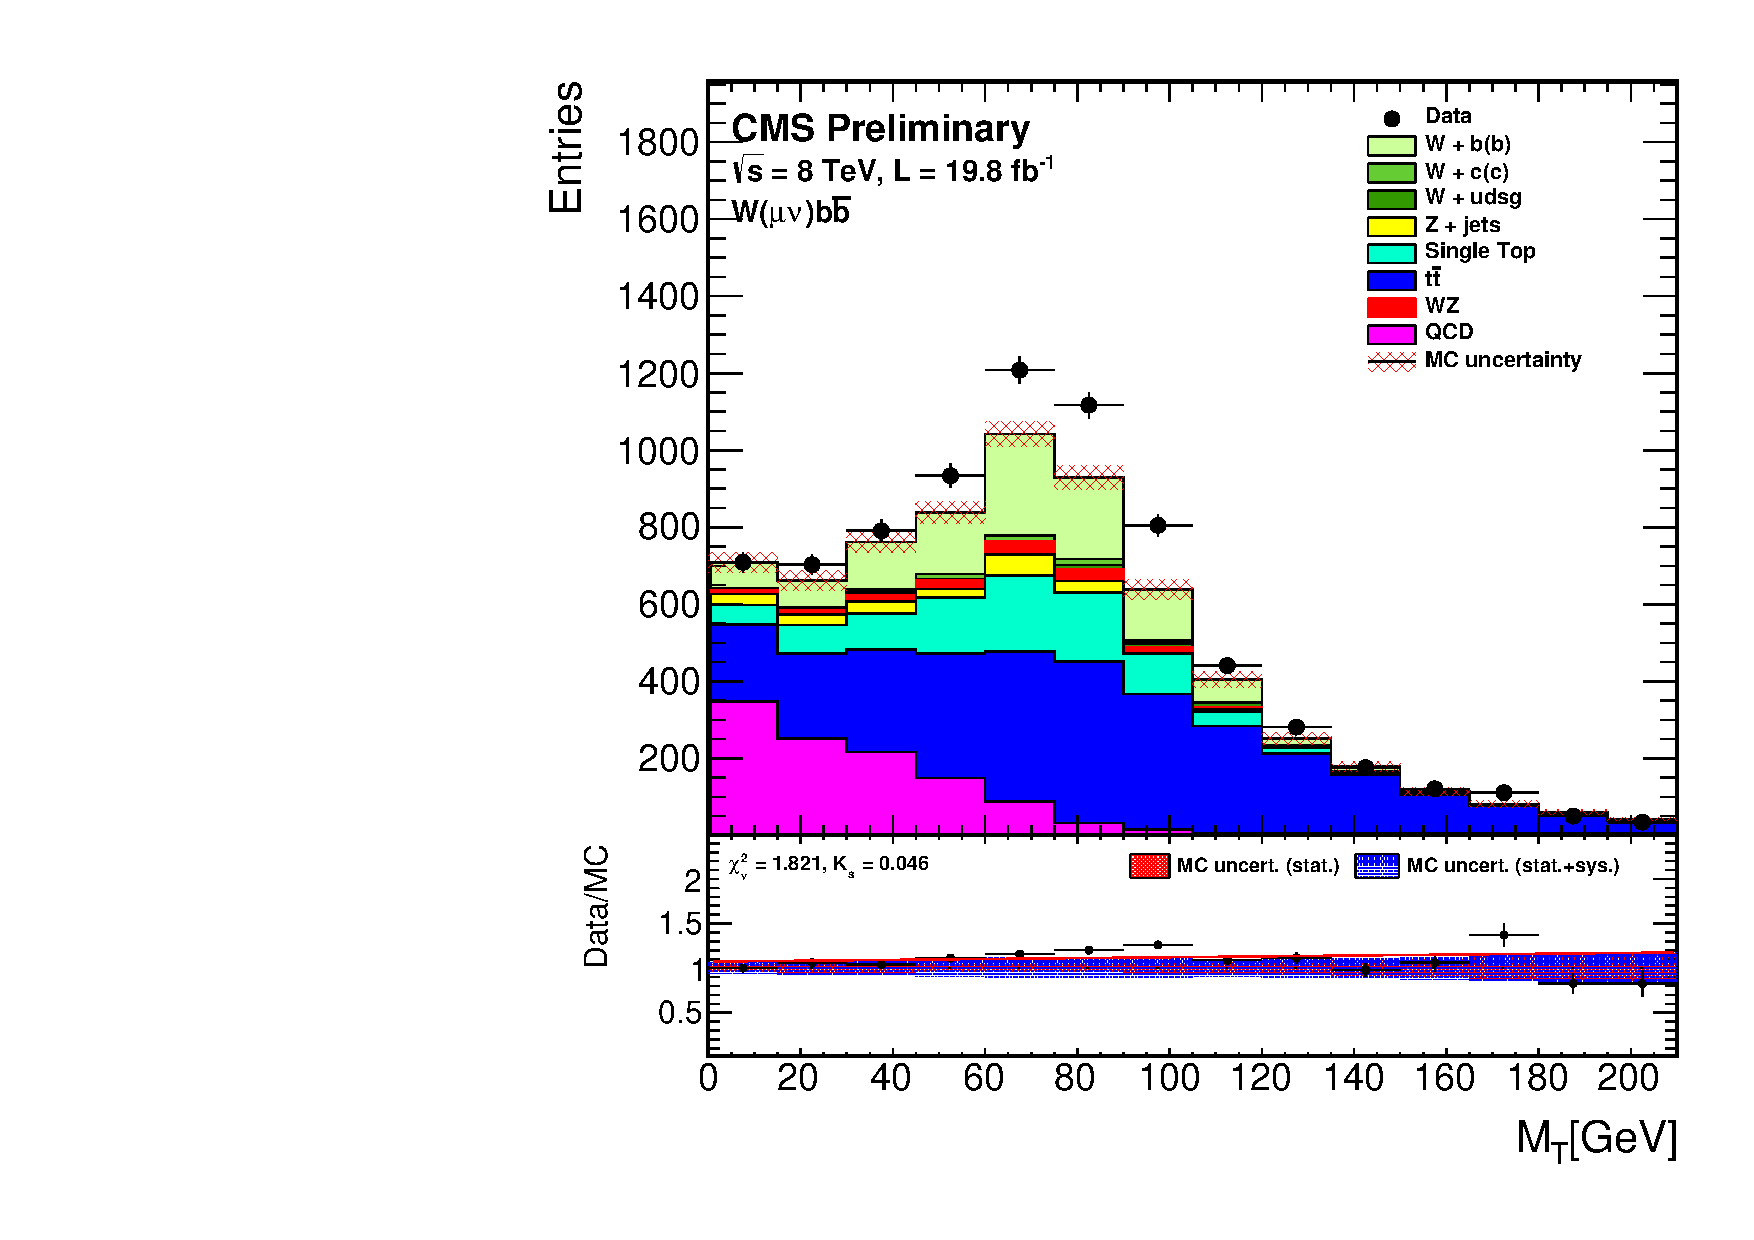
\includegraphics[width=0.48\textwidth]{Figures/Results/Muon/prefit/Wbb_GetVMt_doQCD1.pdf}
		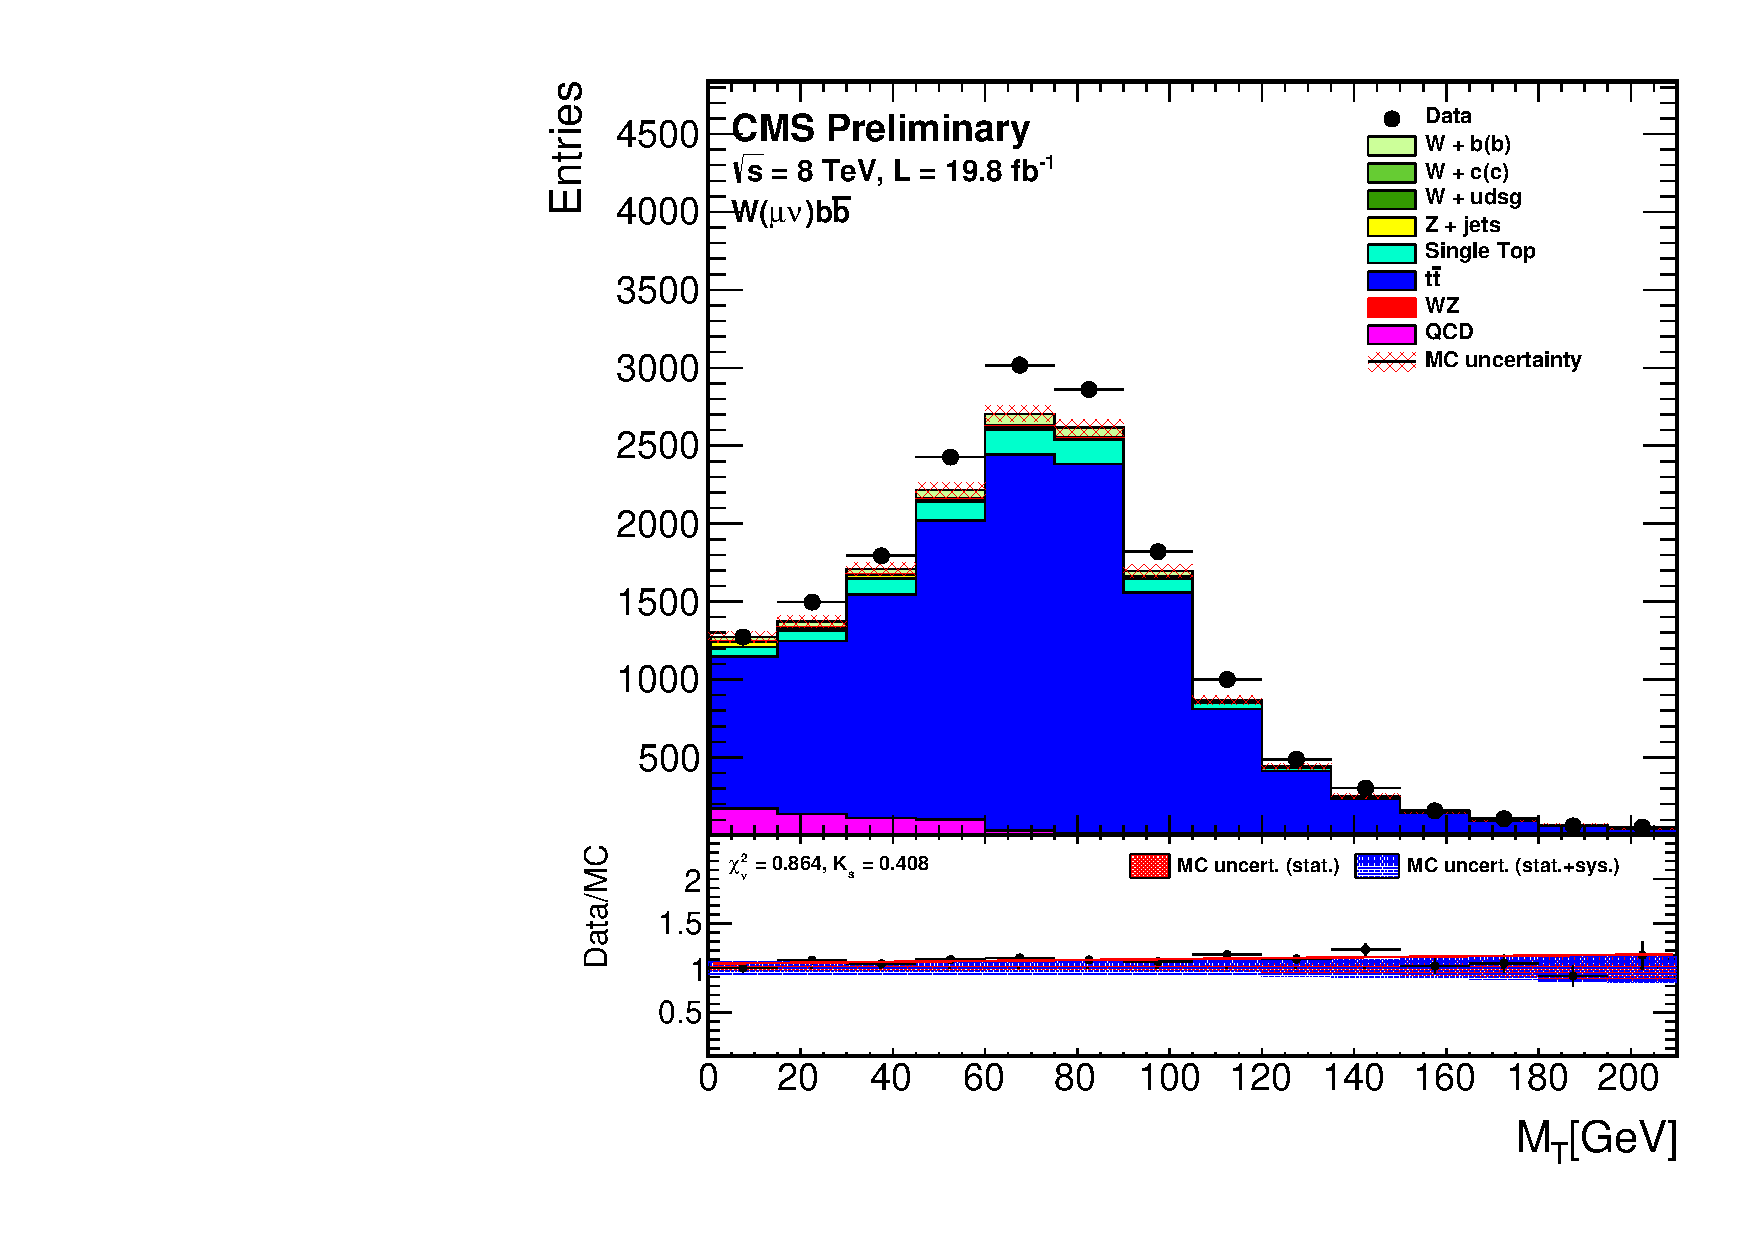
\includegraphics[width=0.48\textwidth]{Figures/Results/Muon/prefit/TT_GetVMt_doQCD1.pdf}
		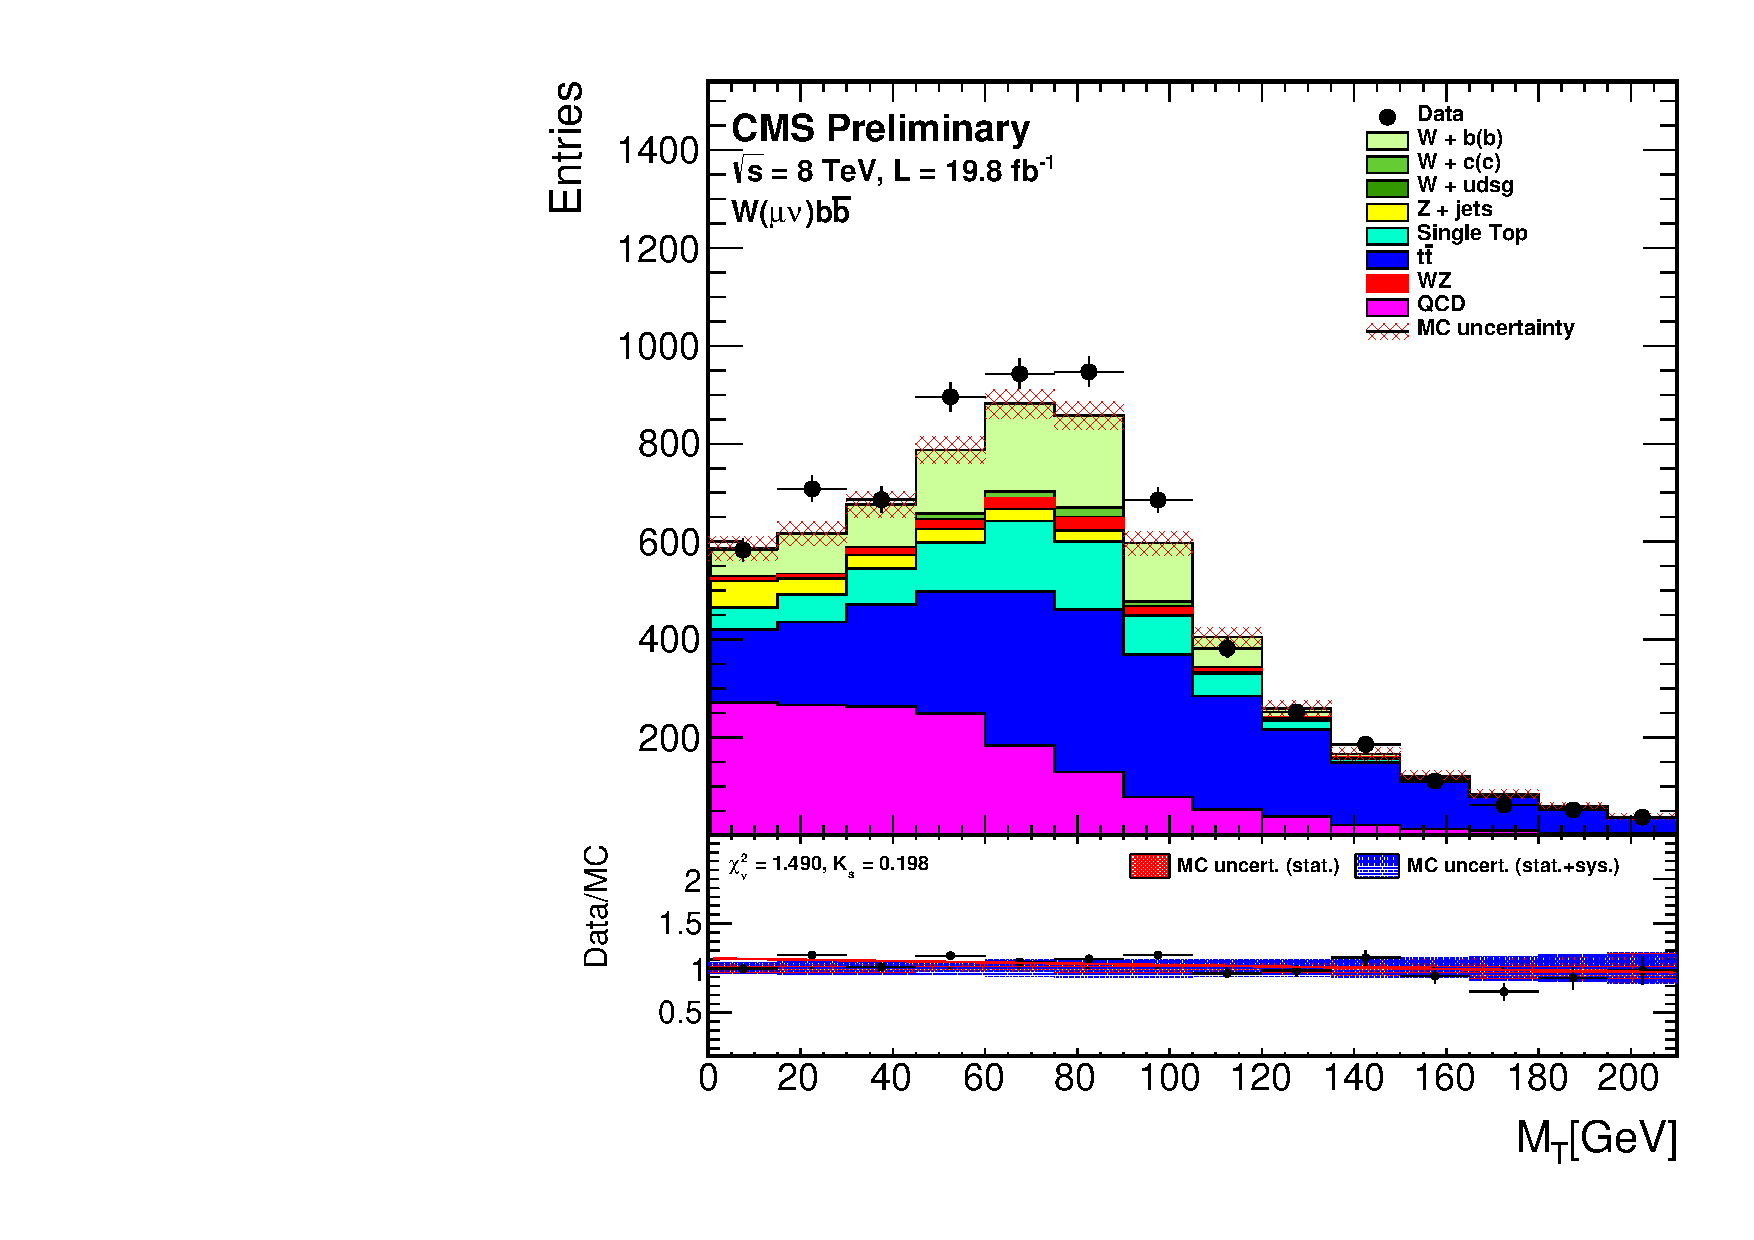
\includegraphics[width=0.48\textwidth]{Figures/Results/Electron/prefit/Wbb_GetVMt_doQCD1.pdf}
		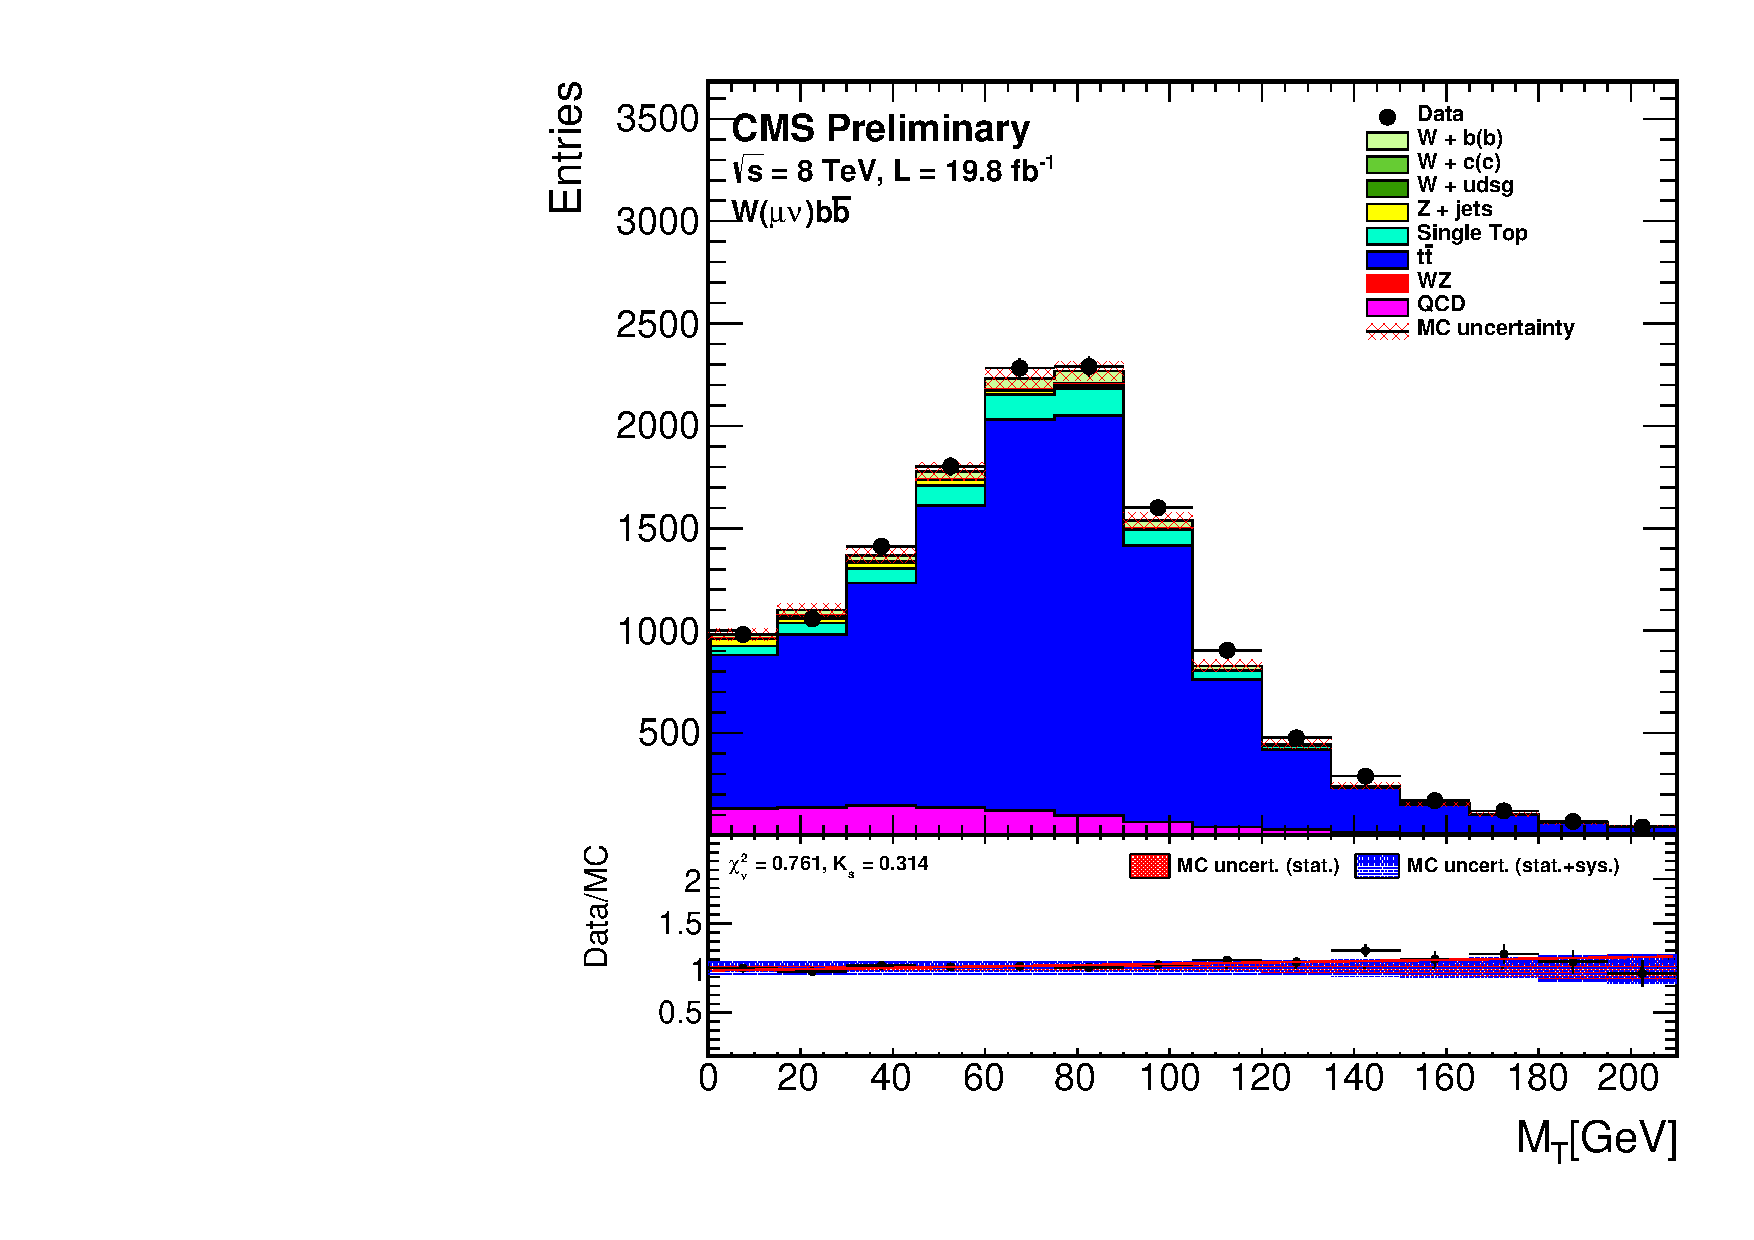
\includegraphics[width=0.48\textwidth]{Figures/Results/Electron/prefit/TT_GetVMt_doQCD1.pdf}
		%\rule{35em}{0.5pt}
	\caption[Transverse mass distributions]{Distribucije transverzne mase za mionski (\textit{gore}) i elektronski (\textit{dolje}) za signalno područje i kontrolno područje dominitanu top kvark pozadinom.}
	\label{fig:mt_hr}
\end{figure}

U konačnoj prilagodbi svi doprinosi variraju unutar neodređenosti osim signala koji je slobodan. Konačni rezultat, iskazan kao omjer mjerenog udarnog presjeka i teorijskog predviđanja (\textit{signal strength}), označava se sa $\mu$ i iznosi:
\begin{align*}
\mu_{mu} &= 1.37 \pm 0.07\mathrm{(stat.)} \pm 0.20 \mathrm{(syst.)}\\\
\mu_{ele} &= 1.67 \pm 0.08\mathrm{(stat.)} \pm 0.27\mathrm{(syst.)}
\end{align*}
Korištenjem relacije \ref{equ:xsec_hr} može se sada odrediti udarni presjek. Broj događaja signala je definiran kao broj događaja prije prilagodbe pomnožen s $\mu$. Aktivni dio detektora i efikasnost se uzimaju iz tablice $\ref{tab:AE_hr}$, a integrirani luminozitet iznosi 19.8 fb$^{-1}$. Dobiveni vrijednost udarnog presjeka je:
\begin{align*}
\sigma(pp\rightarrow W+bb)\times \mathcal{B}(W\rightarrow \mu\nu) = 0.66 \pm 0.03(\mathrm{stat.}) \pm 0.10(\mathrm{syst.})\\
\sigma(pp\rightarrow W+bb)\times \mathcal{B}(W\rightarrow e\nu) = 0.78 \pm 0.04(\mathrm{stat.}) \pm 0.13(\mathrm{syst.})
\end{align*} 
Navedeni rezultati uključuju sve prethodno navedene sistematske neodređenosti. Međutim, u obzir nisu uključene sistematske neodređenosti na određivanje aktivnog dijela detektora i efikasnosti prilikom različitog odabira partonske distribucijske funkcije i varijacije renormalizacijske i faktorizacijske skale.
\par Teorijsko predviđanje određeno je MCFM paketom na NLO preciznost s faktorizacijskom i renormalizacijskom skalom postavljenom na masu W bozona. Uzimajući u obzir i doprinos događaja u kojima su se sudarila po dva partona iz svakog protona (\textit{Double parton scattering - DPS}) \cite{Chatrchyan:2013xxa}, udarni presjek tada iznosi:
\begin{equation*}
\sigma_{TH}(pp\rightarrow W+bb)\times \mathcal{B}(W\rightarrow l\nu) = 0.55 \pm 0.03 \mathrm{(theor.)} \pm 0.02 \mathrm{(DPS)} \mathrm{\ pb}.
\end{equation*}

 

\section{Zaključak}

Ova teza predstavlje rezultate mjerenja udarnog presjeka za produkciju W bozona zajedno s parom mlazova nastalih iz b kvarka u sudarima protona na energiji $\sqrt{s}=$ 8 TeV. Podaci su prikupljeni 2012. godine CMS detektorom i odgovaraju integriranom luminozitetu od 19.8 fb$^{-1}$. Udarni presjek je mjeren posebno u elektronskom i mionskom kanalu, a dva su rezultata kompatibilna unutar neodređenosti. Teorijsko predviđanje za ovaj proces izračunato je pomoću MCFM paketa. Mjerena vrijednost je za jednu standardnu devijaciju viša od predviđene teorijske vrijednosti. Neodređenost mjerenja udarnog presjeka je dominirana sistematskim pogreškama, prvenstveno neodređenošću identifikacije b mlazova. Smanjanje ovih efekata bi omogućilo testiranje predviđanja perturbativne kromodinamike. Daljnja istraživanja ovog i sličnih procesa uključuju i mjerenje diferencijalnog udarnog predjeka u ovisnosti o npr. transverzalnom impulsu vodećeg b mlaza što bi dovelo do unapređenja torijskih modela. Nadalje, mogu se proučavati i stanja u kojim su dva B hadrona u istom mlazu što bi dovelo do boljeg razumijevanja kolinearnih konačnih stanja. 

\end{otherlanguage}


%----------------------------------------------------------------------------------------
%	THESIS CONTENT - APPENDICES
%----------------------------------------------------------------------------------------

\addtocontents{toc}{\vspace{2em}} % Add a gap in the Contents, for aesthetics

\appendix % Cue to tell LaTeX that the following 'chapters' are Appendices

% Include the appendices of the thesis as separate files from the Appendices folder
% Uncomment the lines as you write the Appendices

% Appendix A

\chapter{Lorentz angle measurement in Pixel detector} % Main appendix title

\label{AppendixA} % For referencing this appendix elsewhere, use \ref{AppendixA}

\lhead{Appendix A. \emph{Lorentz angle measurement in Pixel detector}} 

\section{Grazing angle method}
Lorentz angle is measured by using grazing angle method described in detail in \cite{Henrich}. From the individual signals in the detector, using reconstruction algorithms, tracks of muon candidates are obtained. From these reconstructed track it is possible to extract the entry point ($x_{reco}$,$y_{reco}$) to each layer of the detector. 
Distance between reconstructed entry point and the actual hit in the detector is then defined as ($\Delta x$,$\Delta y$):
\begin{equation}
\Delta x = x_{center}-x_{reco}
\end{equation} 
\begin{equation}
\Delta y = y_{center}-y_{reco}
\end{equation} 

where ($x_{center}$,$y_{center}$) is the position of each individual pixel center in the observed cluster. Drift of the electrons can be determined using three impact angles defined in the following way:

\begin{equation}
\text{tan} \alpha = \frac{p_z}{p_x}
\end{equation}
\begin{equation}
\text{tan} \beta = \frac{p_z}{p_y}
\end{equation}
\begin{equation}
\text{tan} \gamma = \frac{p_x}{p_y}
\end{equation}

where $p_x$,$p_y$ and $p_z$ are momentum components in local coordinate system which are calculated from reconstructed track parameters (Fig. \ref{fig:kut}). \\
\begin{figure}[ht!]
\centering
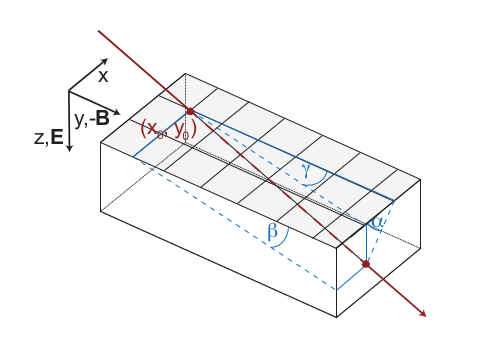
\includegraphics[width=0.5\textwidth]{Figures/kut.png}
\caption{Angle definitions for grazing angle method.}
\label{fig:kut}
\end{figure}
Drift of the electrons depends on the depth at which electrons are created. Depth of the electron production $z$ and drift due to magnetic field $d$ are defined:

\begin{equation}
z = \Delta y \text{ tan}\beta
\end{equation}
\begin{equation}
d=\Delta x-\Delta y \text{ tan}\gamma
\end{equation}

This procedure is repeated for each pixel over many tracks in order to obtain charge drift distance vs depth. The Lorentz angle is the slope of this distribution.  Without a magnetic field, the
direction of the clusters largest extension is parallel to the track projection on the (x, y) plane. The average drift distance of an electron created at a certain depth is obtained from Fig. \ref{fig:2D}. A linear fit is
performed over the total depth of the detector excluding the first and last 50 $\mu$ where the charge drift is systematically displaced by the finite size of the pixel cell (Fig:\ref{fig:profile}). 

\begin{figure}[ht!]
\centering
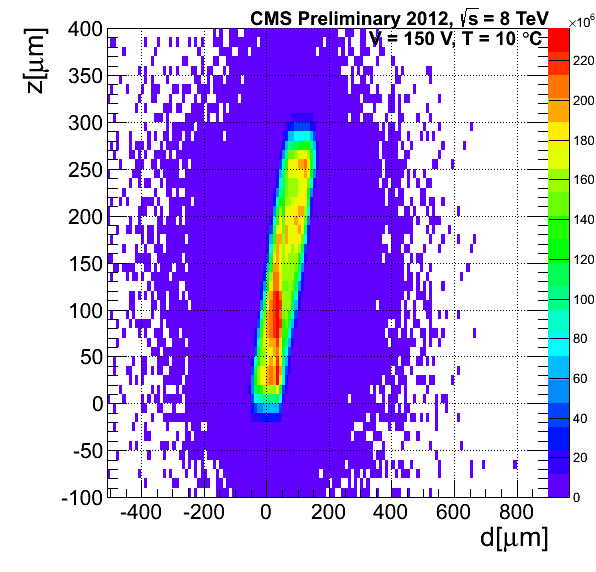
\includegraphics[width=0.5\textwidth]{Figures/LA2012_2D.png}
\caption{Depth at which electrons in silicon bulk were produced as a function of Lorentz drift.}
\label{fig:2D}
\end{figure}

\begin{figure}[ht!]
\centering
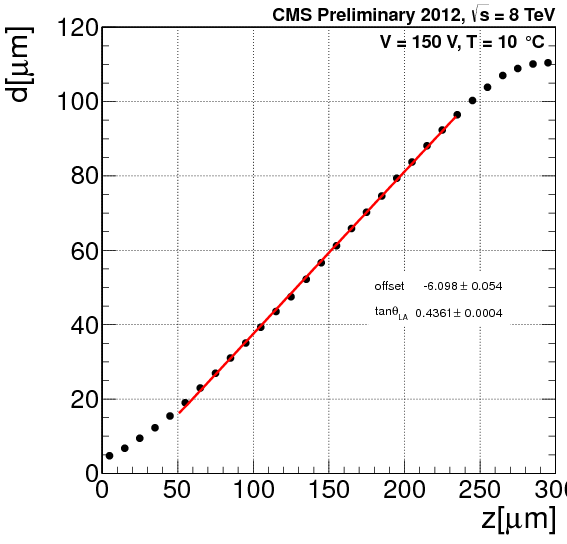
\includegraphics[width=0.5\textwidth]{Figures/LA2012_Profile.png}
\caption{The average drift of electrons as a function of the production depth. Slope of the linear fit result is the $tan \theta_L$.}
\label{fig:profile}
\end{figure}

In order to obtain a good measurement, it is important to use clean tracks. Therefore, it required to have a well reconstructed muon tracks with $p_T>3$GeV and $\chi^2/ndof<2$ which are required to have shallow impact angle with respect to local $y$ direction with cluster size of at least 4 pixels in this direction. Summary of the selection criteria can be found in table \ref{tab:sel}.

\begin{table}[ht!]
  \caption{Selection criteria for Lorentz angle measurement}
  \centering
  \begin{tabular}{l|c}
\hline
\hline
        Cluster size in y & $>3$  \\
	Track $p_t$ & $>3$GeV$/$c \\
	$\chi^2$/ndof & $<2$ \\
	Hit residuals & $<50\mu m$ \\
	Cluster charge & $<120000$e \\
\hline
\hline
  \end{tabular}
  \label{tab:sel}
\end{table}

Figure \ref{fig:La2012} shows how Lorentz angle changes with integrated luminosity. Results are shown for 23fb$^{-1}$ of delivered luminosity in 2012. Increase in Lorentz angle measured with grazing angle method has been observed in all layers, with largest effect (~6\%) visible in layer 1 over this period of data taking.  
\begin{figure}[ht!]
\centering
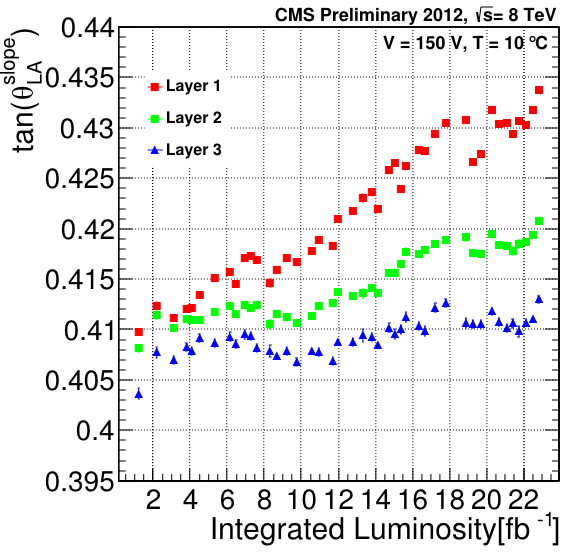
\includegraphics[width=0.5\textwidth]{Figures/LA2012.png}
\caption{Lorentz angle as a function of integrated luminosity for 2012.}
\label{fig:La2012}
\end{figure}

\section{Minimum cluster size method (V-method)}
The pixel cluster size in the drift direction depends on the incident
angle and is minimal when incident angle is equal to the Lorentz angle. Thus, measuring the average cluster size in drift direction as a function of incident angle and obtaining a minimum of that
distribution is an alternative and direct method of measuring the Lorentz angle. The method is usually referred to as V-method due
to a shape of distribution which in the simple case can be approximated with formula

\begin{equation}
p_1*abs(tan(\theta) - p_0) + p_2
\end{equation}
where $p_0$, $p_1$ and $p_2$ are parameters obtained from the fit and $p_0$ = $tan(\theta_{LA})$.

The method was successfully applied to cosmic muon tracks during CMS commissioning period in 2008 and again in 2015. The fit result is shown in figure \ref{fig:LA_VMethod}.

\begin{figure}[hbtp!]
	\centering
	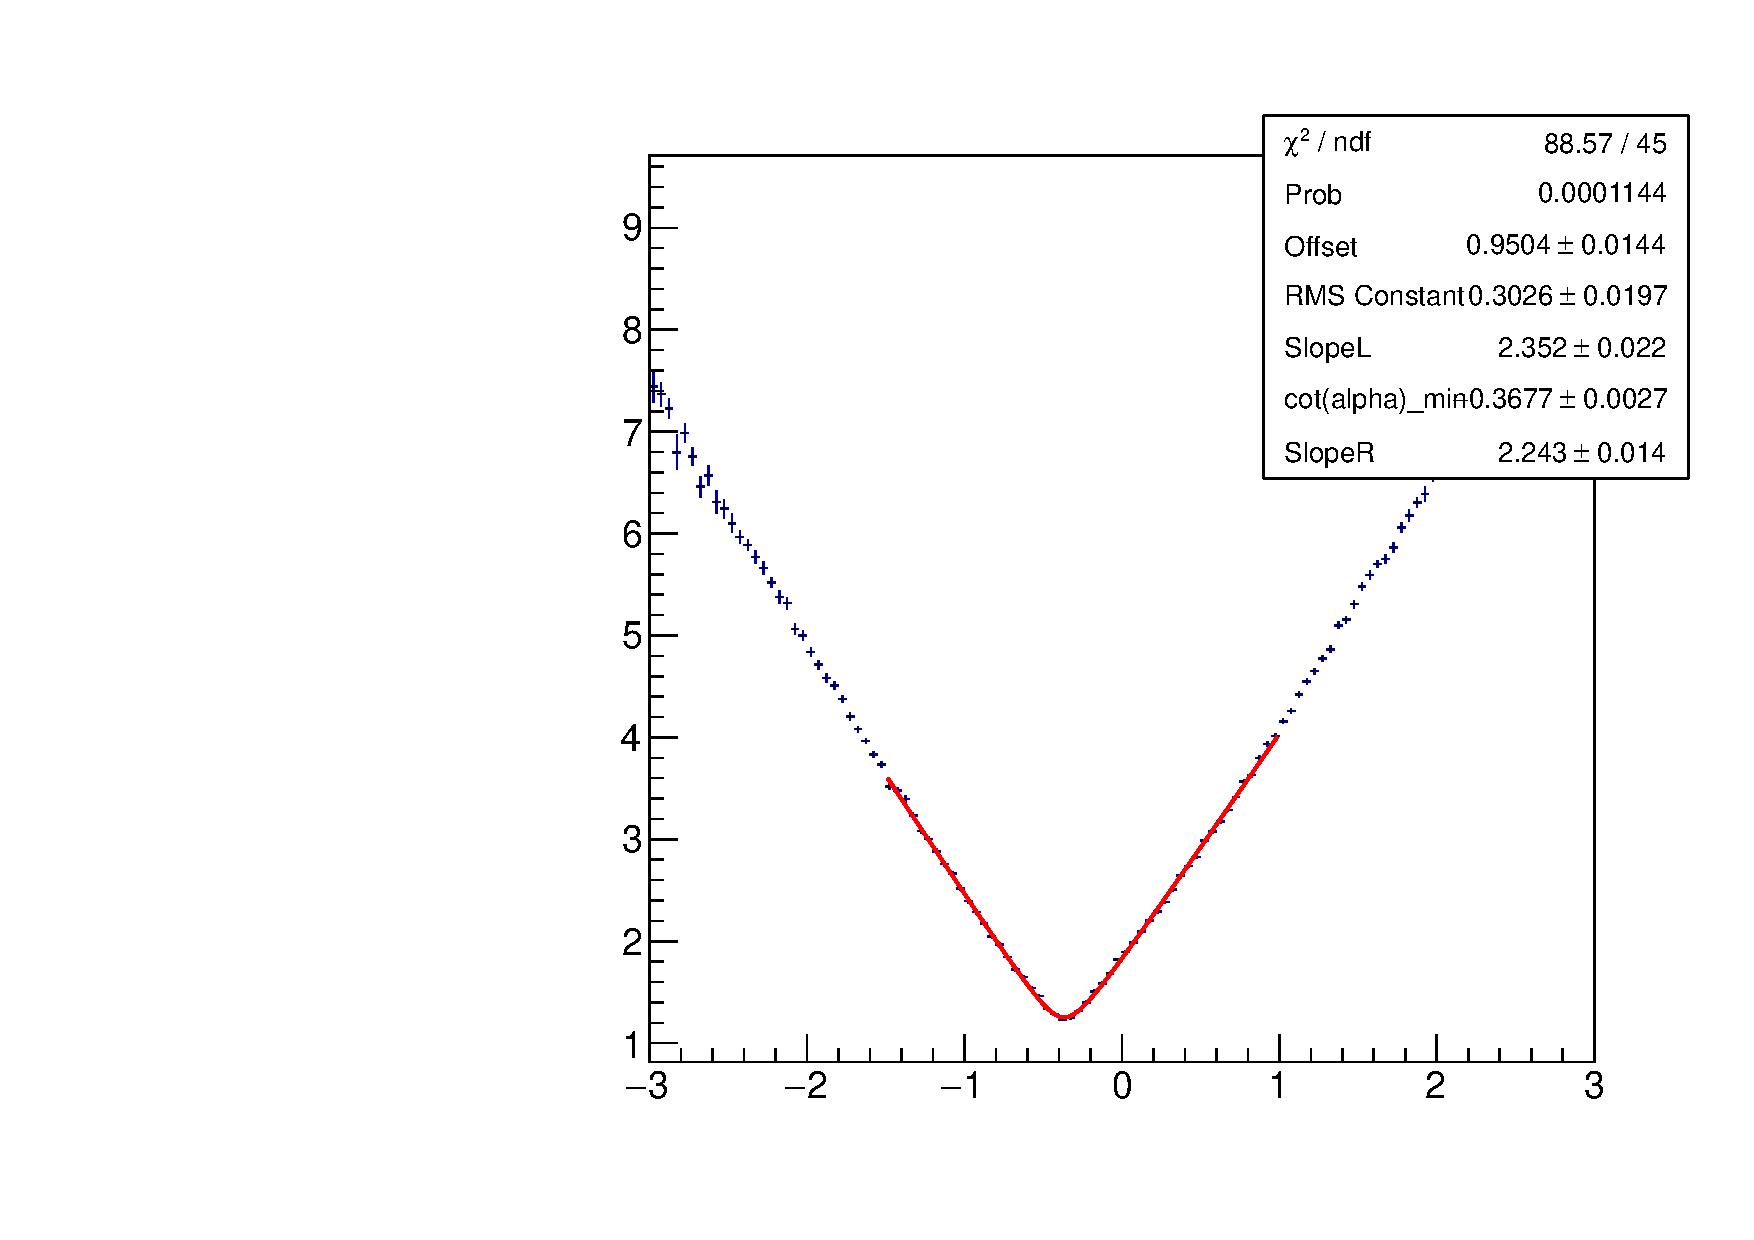
\includegraphics[width=0.5\textwidth]{Figures/LA_VMethod_2015.pdf}
\end{figure}

Application to collision data is more challenging. Coordinates of a track passing through the detector, its incoming angle, and its $p_T$ are
correlated and therefore incoming angles from collision tracks have limited range. With
standard running conditions the value of Lorentz angle is at the edge of that range where tracks with very low $p_T$ (<0.5 GeV) dominate. Because
of that average cluster size as a function of incoming angle cannot be described by a simple model like above mentioned for cosmic data.
While  results for collision data obtained with V-method are in general agreement with the default calculation,  the uncertainty of
the method at present is too big to be used as a viable alternative.


%% Appendix Template

\chapter{Acceptance and efficiency error calculation} % Main appendix title

\label{AppendixB} % Change X to a consecutive letter; for referencing this appendix elsewhere, use \ref{AppendixX}

\lhead{Appendix B. \emph{Acceptance and efficiency error calculation}} % Change X to a consecutive letter; this is for the header on each page - perhaps a shortened title

Write your Appendix content here.
%\input{Appendices/AppendixC}

\addtocontents{toc}{\vspace{2em}} % Add a gap in the Contents, for aesthetics

\backmatter

%----------------------------------------------------------------------------------------
%	BIBLIOGRAPHY
%----------------------------------------------------------------------------------------

\label{Bibliography}

\lhead{\emph{Bibliography}} % Change the page header to say "Bibliography"

%\bibliographystyle{unsrtnat} % Use the "unsrtnat" BibTeX style for formatting the Bibliography
\bibliographystyle{unsrtnat}

\bibliography{Bibliography} % The references (bibliography) information are stored in the file named "Bibliography.bib"

%% LaTeX Curriculum Vitae Template
%%
%% Copyright (C) 2004-2009 Jason Blevins <jrblevin@sdf.lonestar.org>
%% http://jblevins.org/projects/cv-template/
%%
%% You may use use this document as a template to create your own CV
%% and you may redistribute the source code freely. No attribution is
%% required in any resulting documents. I do ask that you please leave
%% this notice and the above URL in the source code if you choose to
%% redistribute this file.
%
%\documentclass[letterpaper,12pt]{article}
%
%\usepackage{hyperref}
%\usepackage{geometry}
%
%
%% Comment the following lines to use the default Computer Modern font
%% instead of the Palatino font provided by the mathpazo package.
%% Remove the 'osf' bit if you don't like the old style figures.
%\usepackage[T1]{fontenc}
%\usepackage[utf8]{inputenc}
%\usepackage[sc]{mathpazo}
%\usepackage[croatian]{babel}
%% Set your name here
%\def\name{Jelena Luetić}
%
%% Replace this with a link to your CV if you like, or set it empty
%% (as in \def\footerlink{}) to remove the link in the footer:
%\def\footerlink{}
%
%% The following metadata will show up in the PDF properties
%\hypersetup{
%  colorlinks = true,
%  urlcolor = black,
%  pdfauthor = {\name},
%  pdfkeywords = {physics, statistics, mathematics},
%  pdftitle = {\name: Curriculum Vitae},
%  pdfsubject = {Curriculum Vitae},
%  pdfpagemode = UseNone
%}
%
%\geometry{
%  body={6.5in, 8.5in},
%  left=1.0in,
%  top=1.25in
%}
%
%% Customize page headers
%\pagestyle{myheadings}
%\markright{\name}
%\thispagestyle{empty}
%
%% Custom section fonts
%\usepackage{sectsty}
%\sectionfont{\rmfamily\mdseries\Large}
%\subsectionfont{\rmfamily\mdseries\itshape\large}
%
%% Other possible font commands include:
%% \ttfamily for teletype,
%% \sffamily for sans serif,
%% \bfseries for bold,
%% \scshape for small caps,
%% \normalsize, \large, \Large, \LARGE sizes.
%
%% Don't indent paragraphs.
%\setlength\parindent{0em}
%
%% Make lists without bullets
%%\renewenvironment{itemize}{
%%  \begin{list}{}{
%%    \setlength{\leftmargin}{1.5em}
%%  }
%%}{
%%  \end{list}
%%}
%
%\begin{document}
%
%% Place name at left
%{\huge \name}
%
%% Alternatively, print name centered and bold:
%%\centerline{\huge \bf \name}
%
%\vspace{0.25in}
%
%%\begin{minipage}{0.45\linewidth}
%%  \href{http://www.irb.hr/}{Ruđer Bošković Institute} \\
%%  Department of experimental physics \\
%%  Bijenička 54, 10000 Zagreb
%%\end{minipage}

\chapter*{Curriculum vitae}
\lhead{\emph{Curriculum vitae}}
\section*{Personal}


  \begin{tabular}{r|l}
    Name & Jelena Luetić \\
	Address & Supilova 7, 10000 Zagreb, Croatia \\   
    Date of Birth & April 5, 1987 \\
    Place of birth & Split, Croatia \\
    Citizenship & Croatian \\
    Phone & +385 91 1480103 \\
    Email & \href{mailto:jelena.luetic@cern.ch}{\tt jelena.luetic@cern.ch} \\
    Languages & English, basic Italian and French, Croatian - native \\
  \end{tabular}



\section*{Education}

\begin{table}[h!]
 \centering
\begin{tabular}{r | l}
2011 - & \textbf{PhD}, Faculty of Science, Physics department \\ & \textit{Title}: 
Measurement of the cross section for associated production of a W boson \\ & and two b quarks with the CMS detector at the Large Hadron Collider \\ &  \textit{Advisor:} Prof. Vuko Brigljević, thesis defence is scheduled for July, 15th 2015. \\[5pt] 
2005 - 2010 & \textbf{MSc}, Faculty of Science, Physics department \\  & \textit{Title}: Measurement of Z boson cross section in proton-proton collisions \\ & with CMS detector at Large Hadron Collider \\ &  \textit{Advisor:} Prof. Ivica Puljak, thesis defended on November, 30th 2010. \\ 
\end{tabular}
\end{table}


\section*{Professional experience}

Since 2009 I've been a part of the CMS group at Ruđer Bošković Institute, working on gauge boson produced in association with jets measurements and on technical aspects of CMS detector:
\begin{itemize}
\item One of the main contributors to Wbb cross section measurement at $\sqrt{s} =$ 8 TeV. Collaboration with University of Wisconsin-Madison, University of Trieste and CERN.
\item Responsible for Lorentz angle monitoring and calibration for CMS Pixel detector.
\item Responsible for development and maintenance of technical tools used in the offline analysis shared with other members of CMS Pixel group.
\item Participated in pixel detector recommissioning during the long shutdown. 
\item Paricipated in CMS Pixel Operations
\end{itemize}



\section*{Teaching}

\begin{tabular}{r | l}
  2011 - 2015 & Faculty of Science, Zagreb, Croatia \\ & Teaching assistant in 2 courses - \textit{Introductory laboratory exercises} (2011.- 2012.) \\ & and \textit{Programming in C} (2011.-2015.) \\[5pt]
  2010 - 2011 & Faculty of Electrical Engineering, Mechanical Engineering and Naval \\ & Architecture in Split, Croatia \\ & Teaching assistant - \textit{Laboratory exercises in Modern physics} 
\end{tabular}

\section*{Schools and Conferences}

\begin{tabular}{r | l}
  2009 & CERN Summer Student Programme, Geneva, Switzerland \\[5pt]
  2010 & CERN School of Computing, London, UK \\[5pt]
  2011 & CMSDAS - Data analysis school, Pisa, Italy \\[5pt]
  2012 & Silicon Detector Workshop, Split, Croatia \\
  	   & \textit{Talk:} Lorentz angle measurement in CMS Pixel detector\\[5pt] 
  2013 & EDIT - Excellence in Detectors, Tsukuba, Japan \\
  	   & \textit{Poster}: CMS Pixel detector and Lorentz angle determination \\[5pt]
  2014 & Fermilab - CERN Hadron Collider School, Fermilab, USA\\
\end{tabular}

\section*{Computer skills}
\begin{itemize}
\item Computer languages: C, C++, Fortran, Python 
\item Software: ROOT, Mathematica, LabView
\end{itemize}

\section*{Other}

Participation in various physics and science outreach programs:
\begin{itemize}
	\item Organization of International Masterclasses: lectures and laboratory exercises for high school students covering various topics in high energy physics.
	\item Participated in several science fairs for general public demonstrating experiments. 
\end{itemize}


\section*{Publications}

\setstretch{1.}
\begin{enumerate}

%%   LIST OF PAPERS
%%   Please comment out anything between here and the
%%   first \item
%%   Please send any updates or corrections to the list to
%%   admin@inspirehep.net
%\cite{Aad:2015zhl}
\item%{Aad:2015zhl}
{\bf ``Combined Measurement of the Higgs Boson Mass in $pp$ Collisions at $\sqrt{s}=7$ and 8 TeV with the ATLAS and CMS Experiments''}, 
G.~Aad {\it et al.}  [ATLAS and CMS Collaborations], 
  %arXiv:1503.07589 [hep-ex]
    %{}10.1103/PhysRevLett.114.191803
Phys.\ Rev.\ Lett.\  {\bf 114}191803 (2015) %(Mar 262015)
%\href{http://inspirehep.net/record/1356276}{HEP entry}
%74 citations counted in INSPIRE as of 02 Jul 2015


%\cite{Khachatryan:2015axa}
\item%{Khachatryan:2015axa}
{\bf ``Search for vector-like T quarks decaying to top quarks and Higgs bosons in the all-hadronic channel using jet substructure''}, 
  V.~Khachatryan {\it et al.}  [CMS Collaboration], 
  %arXiv:1503.01952 [hep-ex]
    %{}10.1007/JHEP06(2015)080
JHEP {\bf 1506}080 (2015) %(Mar 62015)
%\href{http://inspirehep.net/record/1348542}{HEP entry}
%5 citations counted in INSPIRE as of 02 Jul 2015


%\cite{Khachatryan:2015rja}
\item%{Khachatryan:2015rja}
{\bf ``Study of final-state radiation in decays of Z bosons produced in $pp$ collisions at 7 TeV''}, 
  V.~Khachatryan {\it et al.}  [CMS Collaboration], 
  %arXiv:1502.07940 [hep-ex]
    %{}10.1103/PhysRevD.91.092012
Phys.\ Rev.\ D {\bf 91}no. 9092012 (2015) %(Feb 272015)
%\href{http://inspirehep.net/record/1346843}{HEP entry}



%\cite{Khachatryan:2015lwa}
\item%{Khachatryan:2015lwa}
{\bf ``Search for physics beyond the standard model in events with two leptonsjetsand missing transverse momentum in pp collisions at sqrt(s) = 8 TeV''}, 
  V.~Khachatryan {\it et al.}  [CMS Collaboration], 
  %arXiv:1502.06031 [hep-ex]
    %{}10.1007/JHEP04(2015)124
JHEP {\bf 1504}124 (2015) %(Feb 202015)
%\href{http://inspirehep.net/record/1345823}{HEP entry}
%21 citations counted in INSPIRE as of 02 Jul 2015


%\cite{Khachatryan:2015kea}
\item%{Khachatryan:2015kea}
{\bf ``Measurement of the Z$\gamma$ production cross section in pp collisions at 8 TeV and search for anomalous triple gauge boson couplings''}, 
  V.~Khachatryan {\it et al.}  [CMS Collaboration], 
  %arXiv:1502.05664 [hep-ex]
    %{}10.1007/JHEP04(2015)164
JHEP {\bf 1504}164 (2015) %(Feb 192015)
%\href{http://inspirehep.net/record/1345354}{HEP entry}
%2 citations counted in INSPIRE as of 02 Jul 2015


%\cite{Khachatryan:2015xaa}
\item%{Khachatryan:2015xaa}
{\bf ``Nuclear effects on the transverse momentum spectra of charged particles in pPb collisions at $\sqrt{s_{_\mathrm {NN}}} =5.02$ TeV''}, 
  V.~Khachatryan {\it et al.}  [CMS Collaboration], 
  %arXiv:1502.05387 [nucl-ex]
    %{}10.1140/epjc/s10052-015-3435-4
Eur.\ Phys.\ J.\ C {\bf 75}no. 5237 (2015) %(Feb 182015)
%\href{http://inspirehep.net/record/1345263}{HEP entry}
%4 citations counted in INSPIRE as of 02 Jul 2015


%\cite{Khachatryan:2015vra}
\item%{Khachatryan:2015vra}
{\bf ``Searches for supersymmetry using the M$_{T2}$ variable in hadronic events produced in pp collisions at 8 TeV''}, 
  V.~Khachatryan {\it et al.}  [CMS Collaboration], 
  %arXiv:1502.04358 [hep-ex]
    %{}10.1007/JHEP05(2015)078
JHEP {\bf 1505}078 (2015) %(Feb 152015)
%\href{http://inspirehep.net/record/1345027}{HEP entry}
%18 citations counted in INSPIRE as of 02 Jul 2015


%\cite{Khachatryan:2015rra}
\item%{Khachatryan:2015rra}
{\bf ``Measurement of J/$\psi$ and $\psi$(2S) Prompt Double-Differential Cross Sections in pp Collisions at $\sqrt{s}$=7 TeV''}, 
  V.~Khachatryan {\it et al.}  [CMS Collaboration], 
  %arXiv:1502.04155 [hep-ex]
    %{}10.1103/PhysRevLett.114.191802
Phys.\ Rev.\ Lett.\  {\bf 114}no. 19191802 (2015) %(Feb 132015)
%\href{http://inspirehep.net/record/1345023}{HEP entry}
%1 citations counted in INSPIRE as of 02 Jul 2015


%\cite{Khachatryan:2015hwa}
\item%{Khachatryan:2015hwa}
{\bf ``Performance of electron reconstruction and selection with the CMS detector in proton-proton collisions at $\sqrt{s}$ = 8  TeV''}, 
  V.~Khachatryan {\it et al.}  [CMS Collaboration], 
  %arXiv:1502.02701 [physics.ins-det]
    %{}10.1088/1748-0221/10/06/P06005
JINST {\bf 10}no. 06P06005 (2015) %(Feb 92015)
%\href{http://inspirehep.net/record/1343791}{HEP entry}
%25 citations counted in INSPIRE as of 02 Jul 2015


%\cite{Khachatryan:2015ila}
\item%{Khachatryan:2015ila}
{\bf ``Search for a standard model Higgs boson produced in association with a top-quark pair and decaying to bottom quarks using a matrix element method''}, 
  V.~Khachatryan {\it et al.}  [CMS Collaboration], 
  %arXiv:1502.02485 [hep-ex]
    %{}10.1140/epjc/s10052-015-3454-1
Eur.\ Phys.\ J.\ C {\bf 75}no. 6251 (2015) %(Feb 92015)
%\href{http://inspirehep.net/record/1343506}{HEP entry}
%10 citations counted in INSPIRE as of 02 Jul 2015


%\cite{Khachatryan:2015pwa}
\item%{Khachatryan:2015pwa}
{\bf ``Search for supersymmetry using razor variables in events with $b$-tagged jets in $pp$ collisions at $\sqrt{s} =$ 8 TeV''}, 
  V.~Khachatryan {\it et al.}  [CMS Collaboration], 
  %arXiv:1502.00300 [hep-ex]
    %{}10.1103/PhysRevD.91.052018
Phys.\ Rev.\ D {\bf 91}052018 (2015) %(Feb 12015)
%\href{http://inspirehep.net/record/1342447}{HEP entry}
%13 citations counted in INSPIRE as of 02 Jul 2015


%\cite{Khachatryan:2015jha}
\item%{Khachatryan:2015jha}
  {\bf ``Search for decays of stopped long-lived particles produced in proton–proton collisions at $\sqrt{s}= 8\,\text {TeV} $''}, 
  V.~Khachatryan {\it et al.}  [CMS Collaboration], 
  %arXiv:1501.05603 [hep-ex]
    %{}10.1140/epjc/s10052-015-3367-z
Eur.\ Phys.\ J.\ C {\bf 75}no. 4151 (2015) %(Jan 222015)
%\href{http://inspirehep.net/record/1340699}{HEP entry}
%8 citations counted in INSPIRE as of 02 Jul 2015


%\cite{Khachatryan:2015sja}
\item%{Khachatryan:2015sja}
{\bf ``Search for resonances and quantum black holes using dijet mass spectra in proton-proton collisions at $\sqrt{s} =$ 8 TeV''}, 
  V.~Khachatryan {\it et al.}  [CMS Collaboration], 
  %arXiv:1501.04198 [hep-ex]
    %{}10.1103/PhysRevD.91.052009
Phys.\ Rev.\ D {\bf 91}no. 5052009 (2015) %(Jan 172015)
%\href{http://inspirehep.net/record/1340084}{HEP entry}
%27 citations counted in INSPIRE as of 02 Jul 2015


%\cite{Khachatryan:2014jba}
\item%{Khachatryan:2014jba}
{\bf ``Precise determination of the mass of the Higgs boson and tests of compatibility of its couplings with the standard model predictions using proton collisions at 7 and 8 $\,\text {TeV}$''}, 
  V.~Khachatryan {\it et al.}  [CMS Collaboration], 
  %arXiv:1412.8662 [hep-ex]
    %{}10.1140/epjc/s10052-015-3351-7
Eur.\ Phys.\ J.\ C {\bf 75}no. 5212 (2015) %(Dec 302014)
%\href{http://inspirehep.net/record/1335811}{HEP entry}
%124 citations counted in INSPIRE as of 02 Jul 2015


%\cite{Khachatryan:2014lpa}
\item%{Khachatryan:2014lpa}
{\bf ``Search for pair-produced resonances decaying to jet pairs in proton-proton collisions at sqrt(s) = 8 TeV''}, 
  V.~Khachatryan {\it et al.}  [CMS Collaboration], 
  %arXiv:1412.7706 [hep-ex]
    %{}10.1016/j.physletb.2015.04.045
Phys.\ Lett.\ B {\bf 747}98 (2015) %(Dec 242014)
%\href{http://inspirehep.net/record/1335501}{HEP entry}
%14 citations counted in INSPIRE as of 02 Jul 2015


%\cite{Khachatryan:2014fba}
\item%{Khachatryan:2014fba}
{\bf ``Search for physics beyond the standard model in dilepton mass spectra in proton-proton collisions at $ \sqrt{s}=8 $ TeV''}, 
  V.~Khachatryan {\it et al.}  [CMS Collaboration], 
  %arXiv:1412.6302 [hep-ex]
    %{}10.1007/JHEP04(2015)025
JHEP {\bf 1504}025 (2015) %(Dec 192014)
%\href{http://inspirehep.net/record/1335131}{HEP entry}
%25 citations counted in INSPIRE as of 02 Jul 2015


%\cite{CMS:2014dpa}
\item%{CMS:2014dpa}
{\bf ``Searches for supersymmetry based on events with b jets and four W bosons in pp collisions at 8 TeV''}, 
  V.~Khachatryan {\it et al.}  [CMS Collaboration], 
  %arXiv:1412.4109 [hep-ex]
    %{}10.1016/j.physletb.2015.04.002
Phys.\ Lett.\ B {\bf 745}5 (2015) %(Dec 122014)
%\href{http://inspirehep.net/record/1334141}{HEP entry}
%5 citations counted in INSPIRE as of 02 Jul 2015


%\cite{CMS:2014mna}
\item%{CMS:2014mna}
{\bf ``Measurement of the inclusive 3-jet production differential cross section in proton–proton collisions at 7 TeV and determination of the strong coupling constant in the TeV range''}, 
  V.~Khachatryan {\it et al.}  [CMS Collaboration], 
  %arXiv:1412.1633 [hep-ex]
    %{}10.1140/epjc/s10052-015-3376-y
Eur.\ Phys.\ J.\ C {\bf 75}no. 5186 (2015) %(Dec 42014)
%\href{http://inspirehep.net/record/1332746}{HEP entry}
%6 citations counted in INSPIRE as of 02 Jul 2015


%\cite{CMS:2014jea}
\item%{CMS:2014jea}
{\bf ``Measurements of differential and double-differential Drell-Yan cross sections in proton-proton collisions at 8 TeV''}, 
  V.~Khachatryan {\it et al.}  [CMS Collaboration], 
  %arXiv:1412.1115 [hep-ex]
    %{}10.1140/epjc/s10052-015-3364-2
Eur.\ Phys.\ J.\ C {\bf 75}no. 4147 (2015) %(Dec 22014)
%\href{http://inspirehep.net/record/1332509}{HEP entry}
%4 citations counted in INSPIRE as of 02 Jul 2015


%\cite{CMS:2014exa}
\item%{CMS:2014exa}
{\bf ``Search for stealth supersymmetry in events with jetseither photons or leptonsand low missing transverse momentum in pp collisions at 8 TeV''}, 
  V.~Khachatryan {\it et al.}  [CMS Collaboration], 
  %arXiv:1411.7255 [hep-ex]
    %{}10.1016/j.physletb.2015.03.017
Phys.\ Lett.\ B {\bf 743}503 (2015) %(Nov 262014)
%\href{http://inspirehep.net/record/1330294}{HEP entry}
%6 citations counted in INSPIRE as of 02 Jul 2015


%\cite{CMS:2014hka}
\item%{CMS:2014hka}
{\bf ``Search for long-lived particles that decay into final states containing two electrons or two muons in proton-proton collisions at $\sqrt{s} =$ 8 TeV''}, 
  V.~Khachatryan {\it et al.}  [CMS Collaboration], 
  %arXiv:1411.6977 [hep-ex]
    %{}10.1103/PhysRevD.91.052012
Phys.\ Rev.\ D {\bf 91}no. 5052012 (2015) %(Nov 252014)
%\href{http://inspirehep.net/record/1329959}{HEP entry}
%15 citations counted in INSPIRE as of 02 Jul 2015


%\cite{CMS:2014wda}
\item%{CMS:2014wda}
{\bf ``Search for long-lived neutral particles decaying to quark-antiquark pairs in proton-proton collisions at $\sqrt{s} =$ 8 TeV''}, 
  V.~Khachatryan {\it et al.}  [CMS Collaboration], 
  %arXiv:1411.6530 [hep-ex]
    %{}10.1103/PhysRevD.91.012007
Phys.\ Rev.\ D {\bf 91}no. 1012007 (2015) %(Nov 242014)
%\href{http://inspirehep.net/record/1329792}{HEP entry}
%22 citations counted in INSPIRE as of 02 Jul 2015


%\cite{CMS:2014gxa}
\item%{CMS:2014gxa}
{\bf ``Search for disappearing tracks in proton-proton collisions at $ \sqrt{s}=8 $ TeV''}, 
  V.~Khachatryan {\it et al.}  [CMS Collaboration], 
  %arXiv:1411.6006 [hep-ex]
    %{}10.1007/JHEP01(2015)096
JHEP {\bf 1501}096 (2015) %(Nov 212014)
%\href{http://inspirehep.net/record/1329620}{HEP entry}
%20 citations counted in INSPIRE as of 02 Jul 2015


%\cite{CMS:2014yxa}
\item%{CMS:2014yxa}
{\bf ``Measurement of the cross section ratio $\sigma_{ttb\bar{b}}/\sigma_{ttjj}$ in $pp$ collisions at $\sqrt{s} =$ 8 TeV''}, 
  V.~Khachatryan {\it et al.}  [CMS Collaboration], 
  %arXiv:1411.5621 [hep-ex]
    %{}10.1016/j.physletb.2015.04.060
Phys.\ Lett.\ B {\bf 746}132 (2015) %(Nov 202014)
%\href{http://inspirehep.net/record/1328962}{HEP entry}
%1 citations counted in INSPIRE as of 02 Jul 2015


%\cite{CMS:2014xfa}
\item%{CMS:2014xfa}
{\bf ``Observation of the rare $B^0_s\to\mu^+\mu^-$ decay from the combined analysis of CMS and LHCb data''}, 
  V.~Khachatryan {\it et al.}  [CMS and LHCb Collaborations], 
  %arXiv:1411.4413 [hep-ex]
    %{}10.1038/nature14474
Nature {\bf 522}68 (2015) %(Nov 172014)
%\href{http://inspirehep.net/record/1328493}{HEP entry}
%50 citations counted in INSPIRE as of 02 Jul 2015


%\cite{Khachatryan:2014cja}
\item%{Khachatryan:2014cja}
{\bf ``Search for quark contact interactions and extra spatial dimensions using dijet angular distributions in proton–proton collisions at $\sqrt{s} =$ 8 TeV''}, 
  V.~Khachatryan {\it et al.}  [CMS Collaboration], 
  %arXiv:1411.2646 [hep-ex]
    %{}10.1016/j.physletb.2015.04.042
Phys.\ Lett.\ B {\bf 746}79 (2015) %(Nov 102014)
%\href{http://inspirehep.net/record/1327224}{HEP entry}
%9 citations counted in INSPIRE as of 02 Jul 2015


%\cite{Khachatryan:2014gga}
\item%{Khachatryan:2014gga}
{\bf ``Performance of the CMS missing transverse momentum reconstruction in pp data at $\sqrt{s}$ = 8 TeV''}, 
  V.~Khachatryan {\it et al.}  [CMS Collaboration], 
  %arXiv:1411.0511 [physics.ins-det]
    %{}10.1088/1748-0221/10/02/P02006
JINST {\bf 10}no. 02P02006 (2015) %(Nov 32014)
%\href{http://inspirehep.net/record/1325798}{HEP entry}
%5 citations counted in INSPIRE as of 02 Jul 2015


%\cite{Khachatryan:2014waa}
\item%{Khachatryan:2014waa}
{\bf ``Constraints on parton distribution functions and extraction of the strong coupling constant from the inclusive jet cross section in pp collisions at $\sqrt{s} = 7$ $\,\text {TeV}$''}, 
  V.~Khachatryan {\it et al.}  [CMS Collaboration], 
  %arXiv:1410.6765 [hep-ex]
    %{}10.1140/epjc/s10052-015-3499-1
Eur.\ Phys.\ J.\ C {\bf 75}no. 6288 (2015) %(Oct 242014)
%\href{http://inspirehep.net/record/1323630}{HEP entry}
%12 citations counted in INSPIRE as of 02 Jul 2015


%\cite{Khachatryan:2014aep}
\item%{Khachatryan:2014aep}
{\bf ``Search for a standard model$-$like Higgs boson in the $\mu ^{+}\mu ^{-}$ and $e^{+}e^{-}$ decay channels at the LHC''}, 
  V.~Khachatryan {\it et al.}  [CMS Collaboration], 
  %arXiv:1410.6679 [hep-ex]
    %{}10.1016/j.physletb.2015.03.048
Phys.\ Lett.\ B {\bf 744}184 (2015) %(Oct 242014)
%\href{http://inspirehep.net/record/1323624}{HEP entry}
%21 citations counted in INSPIRE as of 02 Jul 2015


%\cite{Khachatryan:2014sta}
\item%{Khachatryan:2014sta}
{\bf ``Study of vector boson scattering and search for new physics in events with two same-sign leptons and two jets''}, 
  V.~Khachatryan {\it et al.}  [CMS Collaboration], 
  %arXiv:1410.6315 [hep-ex]
    %{}10.1103/PhysRevLett.114.051801
Phys.\ Rev.\ Lett.\  {\bf 114}no. 5051801 (2015) %(Oct 232014)
%\href{http://inspirehep.net/record/1323444}{HEP entry}
%10 citations counted in INSPIRE as of 02 Jul 2015


%\cite{Khachatryan:2014nfa}
\item%{Khachatryan:2014nfa}
{\bf ``Measurement of the ratio of the production cross sections times branching fractions of $B_{c}^{\pm} \to J/\psi \pi^{\pm}$ and $B^{\pm} \to J/\psi K^{\pm}$ and $\mathcal{B}(B_{c}^{\pm} \to J/\psi \pi^{\pm}\pi^{\pm}\pi^{\mp})/\mathcal{B}(B_{c}^{\pm} \to J/\psi \pi^{\pm})$ in pp collisions at $\sqrt{s} =$ 7 TeV''}, 
  V.~Khachatryan {\it et al.}  [CMS Collaboration], 
  %arXiv:1410.5729 [hep-ex]
    %{}10.1007/JHEP01(2015)063
JHEP {\bf 1501}063 (2015) %(Oct 212014)
%\href{http://inspirehep.net/record/1323075}{HEP entry}
%2 citations counted in INSPIRE as of 02 Jul 2015


%\cite{Chatrchyan:2014csa}
\item%{Chatrchyan:2014csa}
{\bf ``Study of Z production in PbPb and pp collisions at $ \sqrt{s_{\mathrm{NN}}}=2.76 $ TeV in the dimuon and dielectron decay channels''}, 
  S.~Chatrchyan {\it et al.}  [CMS Collaboration], 
  %arXiv:1410.4825 [nucl-ex]
    %{}10.1007/JHEP03(2015)022
JHEP {\bf 1503}022 (2015) %(Oct 172014)
%\href{http://inspirehep.net/record/1322726}{HEP entry}
%6 citations counted in INSPIRE as of 02 Jul 2015


%\cite{Khachatryan:2014vla}
\item%{Khachatryan:2014vla}
{\bf ``Identification techniques for highly boosted W bosons that decay into hadrons''}, 
  V.~Khachatryan {\it et al.}  [CMS Collaboration], 
  %arXiv:1410.4227 [hep-ex]
    %{}10.1007/JHEP12(2014)017
JHEP {\bf 1412}017 (2014) %(Oct 152014)
%\href{http://inspirehep.net/record/1322563}{HEP entry}
%12 citations counted in INSPIRE as of 02 Jul 2015


%\cite{Khachatryan:2014dea}
\item%{Khachatryan:2014dea}
{\bf ``Measurement of electroweak production of two jets in association with a Z boson in proton-proton collisions at $\sqrt{s}=8\,\text {TeV}$''}, 
  V.~Khachatryan {\it et al.}  [CMS Collaboration], 
  %arXiv:1410.3153 [hep-ex]
    %{}10.1140/epjc/s10052-014-3232-5
Eur.\ Phys.\ J.\ C {\bf 75}no. 266 (2015) %(Oct 122014)
%\href{http://inspirehep.net/record/1321687}{HEP entry}
%7 citations counted in INSPIRE as of 02 Jul 2015


%\cite{Khachatryan:2014jya}
\item%{Khachatryan:2014jya}
{\bf ``Searches for heavy Higgs bosons in two-Higgs-doublet models and for $t\rightarrow ch$ decay using multilepton and diphoton final states in $pp$ collisions at 8 TeV''}, 
  V.~Khachatryan {\it et al.}  [CMS Collaboration], 
  %arXiv:1410.2751 [hep-ex]
    %{}10.1103/PhysRevD.90.112013
Phys.\ Rev.\ D {\bf 90}112013 (2014) %(Oct 102014)
%\href{http://inspirehep.net/record/1321537}{HEP entry}
%18 citations counted in INSPIRE as of 02 Jul 2015


%\cite{Khachatryan:2014bva}
\item%{Khachatryan:2014bva}
{\bf ``Measurement of Prompt $\psi(2S) \to J/\psi$ Yield Ratios in Pb-Pb and $p-p$ Collisions at $\sqrt {s_{NN}}=$ 2.76 TeV''}, 
  V.~Khachatryan {\it et al.}  [CMS Collaboration], 
  %arXiv:1410.1804 [nucl-ex]
    %{}10.1103/PhysRevLett.113.262301
Phys.\ Rev.\ Lett.\  {\bf 113}no. 26262301 (2014) %(Oct 72014)
%\href{http://inspirehep.net/record/1320775}{HEP entry}
%7 citations counted in INSPIRE as of 02 Jul 2015


%\cite{Khachatryan:2014vma}
\item%{Khachatryan:2014vma}
{\bf ``Measurement of the W boson helicity in events with a single reconstructed top quark in pp collisions at $ \sqrt{s}=8 $ TeV''}, 
  V.~Khachatryan {\it et al.}  [CMS Collaboration], 
  %arXiv:1410.1154 [hep-ex]
    %{}10.1007/JHEP01(2015)053
JHEP {\bf 1501}053 (2015) %(Oct 52014)
%\href{http://inspirehep.net/record/1320561}{HEP entry}
%6 citations counted in INSPIRE as of 02 Jul 2015


%\cite{Khachatryan:2014uma}
\item%{Khachatryan:2014uma}
{\bf ``Search for Monotop Signatures in Proton-Proton Collisions at $\sqrt s =$ 8 TeV''}, 
  V.~Khachatryan {\it et al.}  [CMS Collaboration], 
  %arXiv:1410.1149 [hep-ex]
    %{}10.1103/PhysRevLett.114.101801
Phys.\ Rev.\ Lett.\  {\bf 114}no. 10101801 (2015) %(Oct 52014)
%\href{http://inspirehep.net/record/1320560}{HEP entry}
%12 citations counted in INSPIRE as of 02 Jul 2015


%\cite{Khachatryan:2014sca}
\item%{Khachatryan:2014sca}
{\bf ``Search for standard model production of four top quarks in the lepton + jets channel in pp collisions at $\sqrt{s}$ = 8 TeV''}, 
  V.~Khachatryan {\it et al.}  [CMS Collaboration], 
  %arXiv:1409.7339 [hep-ex]
    %{}10.1007/JHEP11(2014)154
JHEP {\bf 1411}154 (2014) %(Sep 252014)
%\href{http://inspirehep.net/record/1318946}{HEP entry}
%10 citations counted in INSPIRE as of 02 Jul 2015


%\cite{Khachatryan:2014ofa}
\item%{Khachatryan:2014ofa}
{\bf ``Measurement of the production cross section ratio sigma(chi[b2](1P)) / sigma(chi[b1](1P)) in pp collisions at sqrt(s) = 8 TeV''}, 
  V.~Khachatryan {\it et al.}  [CMS Collaboration], 
  %arXiv:1409.5761 [hep-ex]
    %{}10.1016/j.physletb.2015.02.048
Phys.\ Lett.\ B {\bf 743}383 (2015) %(Sep 192014)
%\href{http://inspirehep.net/record/1318344}{HEP entry}
%3 citations counted in INSPIRE as of 02 Jul 2015


%\cite{Khachatryan:2014mea}
\item%{Khachatryan:2014mea}
{\bf ``Search for Displaced Supersymmetry in events with an electron and a muon with large impact parameters''}, 
  V.~Khachatryan {\it et al.}  [CMS Collaboration], 
  %arXiv:1409.4789 [hep-ex]
    %{}10.1103/PhysRevLett.114.061801
Phys.\ Rev.\ Lett.\  {\bf 114}no. 6061801 (2015) %(Sep 162014)
%\href{http://inspirehep.net/record/1317640}{HEP entry}
%14 citations counted in INSPIRE as of 02 Jul 2015


%\cite{Khachatryan:2014jra}
\item%{Khachatryan:2014jra}
{\bf ``Long-range two-particle correlations of strange hadrons with charged particles in pPb and PbPb collisions at LHC energies''}, 
  V.~Khachatryan {\it et al.}  [CMS Collaboration], 
  %arXiv:1409.3392 [nucl-ex]
    %{}10.1016/j.physletb.2015.01.034
Phys.\ Lett.\ B {\bf 742}200 (2015) %(Sep 112014)
%\href{http://inspirehep.net/record/1315947}{HEP entry}
%12 citations counted in INSPIRE as of 02 Jul 2015


%\cite{Khachatryan:2014mma}
\item%{Khachatryan:2014mma}
{\bf ``Searches for electroweak neutralino and chargino production in channels with HiggsZand W bosons in pp collisions at 8 TeV''}, 
  V.~Khachatryan {\it et al.}  [CMS Collaboration], 
  %arXiv:1409.3168 [hep-ex]
    %{}10.1103/PhysRevD.90.092007
Phys.\ Rev.\ D {\bf 90}no. 9092007 (2014) %(Sep 102014)
%\href{http://inspirehep.net/record/1315820}{HEP entry}
%29 citations counted in INSPIRE as of 02 Jul 2015


%\cite{Khachatryan:2014rra}
\item%{Khachatryan:2014rra}
{\bf ``Search for dark matterextra dimensionsand unparticles in monojet events in proton–proton collisions at $\sqrt{s} = 8$ TeV''}, 
  V.~Khachatryan {\it et al.}  [CMS Collaboration], 
  %arXiv:1408.3583 [hep-ex]
    %{}10.1140/epjc/s10052-015-3451-4
Eur.\ Phys.\ J.\ C {\bf 75}no. 5235 (2015) %(Aug 152014)
%\href{http://inspirehep.net/record/1311223}{HEP entry}
%82 citations counted in INSPIRE as of 02 Jul 2015


%\cite{Khachatryan:2014wca}
\item%{Khachatryan:2014wca}
{\bf ``Search for neutral MSSM Higgs bosons decaying to a pair of tau leptons in pp collisions''}, 
  V.~Khachatryan {\it et al.}  [CMS Collaboration], 
  %arXiv:1408.3316 [hep-ex]
    %{}10.1007/JHEP10(2014)160
JHEP {\bf 1410}160 (2014) %(Aug 142014)
%\href{http://inspirehep.net/record/1310838}{HEP entry}
%65 citations counted in INSPIRE as of 02 Jul 2015


%\cite{Khachatryan:2014zya}
\item%{Khachatryan:2014zya}
{\bf ``Measurements of jet multiplicity and differential production cross sections of $Z +$ jets events in proton-proton collisions at $\sqrt{s} =$ 7 TeV''}, 
  V.~Khachatryan {\it et al.}  [CMS Collaboration], 
  %arXiv:1408.3104 [hep-ex]
    %{}10.1103/PhysRevD.91.052008
Phys.\ Rev.\ D {\bf 91}no. 5052008 (2015) %(Aug 132014)
%\href{http://inspirehep.net/record/1310737}{HEP entry}
%6 citations counted in INSPIRE as of 02 Jul 2015


%\cite{Khachatryan:2014tva}
\item%{Khachatryan:2014tva}
{\bf ``Search for physics beyond the standard model in final states with a lepton and missing transverse energy in proton-proton collisions at sqrt(s) = 8 TeV''}, 
  V.~Khachatryan {\it et al.}  [CMS Collaboration], 
  %arXiv:1408.2745 [hep-ex]
    %{}10.1103/PhysRevD.91.092005
Phys.\ Rev.\ D {\bf 91}no. 9092005 (2015) %(Aug 122014)
%\href{http://inspirehep.net/record/1310653}{HEP entry}
%40 citations counted in INSPIRE as of 02 Jul 2015


%\cite{Khachatryan:2014qaa}
\item%{Khachatryan:2014qaa}
{\bf ``Search for the associated production of the Higgs boson with a top-quark pair''}, 
  V.~Khachatryan {\it et al.}  [CMS Collaboration], 
  %arXiv:1408.1682 [hep-ex]
    %{}10.1007/JHEP09(2014)08710.1007/JHEP10(2014)106
JHEP {\bf 1409}087 (2014)[JHEP {\bf 1410}106 (2014)] %(Aug 72014)
%\href{http://inspirehep.net/record/1310104}{HEP entry}
%47 citations counted in INSPIRE as of 02 Jul 2015


%\cite{Khachatryan:2014ura}
\item%{Khachatryan:2014ura}
{\bf ``Search for pair production of third-generation scalar leptoquarks and top squarks in proton-proton collisions at sqrt(s) = 8 TeV''}, 
  V.~Khachatryan {\it et al.}  [CMS Collaboration], 
  %arXiv:1408.0806 [hep-ex]
    %{}10.1016/j.physletb.2014.10.063
Phys.\ Lett.\ B {\bf 739}229 (2014) %(Aug 42014)
%\href{http://inspirehep.net/record/1309874}{HEP entry}
%25 citations counted in INSPIRE as of 02 Jul 2015


%\cite{Khachatryan:2014loa}
\item%{Khachatryan:2014loa}
{\bf ``Measurement of the $t \bar t$ production cross section in $pp$ collisions at $\sqrt s = 8$ TeV in dilepton final states containing one $\tau$ lepton''}, 
  V.~Khachatryan {\it et al.}  [CMS Collaboration], 
  %arXiv:1407.6643 [hep-ex]
    %{}10.1016/j.physletb.2014.10.032
Phys.\ Lett.\ B {\bf 739}23 (2014) %(Jul 242014)
%\href{http://inspirehep.net/record/1307759}{HEP entry}
%6 citations counted in INSPIRE as of 02 Jul 2015


%\cite{Khachatryan:2014dka}
\item%{Khachatryan:2014dka}
{\bf ``Search for heavy neutrinos and $\mathrm {W}$ bosons with right-handed couplings in proton-proton collisions at $\sqrt{s} = 8\,\text {TeV} $''}, 
  V.~Khachatryan {\it et al.}  [CMS Collaboration], 
  %arXiv:1407.3683 [hep-ex]
    %{}10.1140/epjc/s10052-014-3149-z
Eur.\ Phys.\ J.\ C {\bf 74}no. 113149 (2014) %(Jul 142014)
%\href{http://inspirehep.net/record/1306295}{HEP entry}
%58 citations counted in INSPIRE as of 02 Jul 2015


%\cite{Khachatryan:2014xja}
\item%{Khachatryan:2014xja}
{\bf ``Search for new resonances decaying via WZ to leptons in proton-proton collisions at $\sqrt s =$ 8 TeV''}, 
  V.~Khachatryan {\it et al.}  [CMS Collaboration], 
  %arXiv:1407.3476 [hep-ex]
    %{}10.1016/j.physletb.2014.11.026
Phys.\ Lett.\ B {\bf 740}83 (2015) %(Jul 132014)
%\href{http://inspirehep.net/record/1306289}{HEP entry}
%22 citations counted in INSPIRE as of 02 Jul 2015


%\cite{Khachatryan:2014ika}
\item%{Khachatryan:2014ika}
{\bf ``Study of hadronic event-shape variables in multijet final states in pp collisions at sqrt(s) = 7 TeV''}, 
  V.~Khachatryan {\it et al.}  [CMS Collaboration], 
  %arXiv:1407.2856 [hep-ex]
    %{}10.1007/JHEP10(2014)087
JHEP {\bf 1410}87 (2014) %(Jul 102014)
%\href{http://inspirehep.net/record/1305624}{HEP entry}
%4 citations counted in INSPIRE as of 02 Jul 2015


%\cite{Khachatryan:2014ira}
\item%{Khachatryan:2014ira}
{\bf ``Observation of the diphoton decay of the Higgs boson and measurement of its properties''}, 
  V.~Khachatryan {\it et al.}  [CMS Collaboration], 
  %arXiv:1407.0558 [hep-ex]
    %{}10.1140/epjc/s10052-014-3076-z
Eur.\ Phys.\ J.\ C {\bf 74}no. 103076 (2014) %(Jul 22014)
%\href{http://inspirehep.net/record/1304454}{HEP entry}
%162 citations counted in INSPIRE as of 02 Jul 2015


%\cite{Khachatryan:2014ewa}
\item%{Khachatryan:2014ewa}
{\bf ``Measurement of top quark-antiquark pair production in association with a W or Z boson in pp collisions at $\sqrt{s} = 8$ $\,\text {TeV}$''}, 
  V.~Khachatryan {\it et al.}  [CMS Collaboration], 
  %arXiv:1406.7830 [hep-ex]
    %{}10.1140/epjc/s10052-014-3060-7
Eur.\ Phys.\ J.\ C {\bf 74}no. 93060 (2014) %(Jun 302014)
%\href{http://inspirehep.net/record/1303904}{HEP entry}
%22 citations counted in INSPIRE as of 02 Jul 2015


%\cite{Khachatryan:2014uva}
\item%{Khachatryan:2014uva}
{\bf ``Differential cross section measurements for the production of a W boson in association with jets in proton–proton collisions at $\sqrt s=7$ TeV''}, 
  V.~Khachatryan {\it et al.}  [CMS Collaboration], 
  %arXiv:1406.7533 [hep-ex]
    %{}10.1016/j.physletb.2014.12.003
Phys.\ Lett.\ B {\bf 741}12 (2015) %(Jun 292014)
%\href{http://inspirehep.net/record/1303894}{HEP entry}
%16 citations counted in INSPIRE as of 02 Jul 2015


%\cite{Khachatryan:2014aka}
\item%{Khachatryan:2014aka}
{\bf ``Search for excited quarks in the $\gamma +$jet final state in proton–proton collisions at $\sqrt s=8$ TeV''}, 
  V.~Khachatryan {\it et al.}  [CMS Collaboration], 
  %arXiv:1406.5171 [hep-ex]
    %{}10.1016/j.physletb.2014.09.048
Phys.\ Lett.\ B {\bf 738}274 (2014) %(Jun 192014)
%\href{http://inspirehep.net/record/1301560}{HEP entry}
%9 citations counted in INSPIRE as of 02 Jul 2015


%\cite{Chatrchyan:2014ava}
\item%{Chatrchyan:2014ava}
{\bf ``Measurement of jet fragmentation in PbPb and pp collisions at $\sqrt{s_{NN}}=2.76$ TeV''}, 
  S.~Chatrchyan {\it et al.}  [CMS Collaboration], 
  %arXiv:1406.0932 [nucl-ex]
    %{}10.1103/PhysRevC.90.024908
Phys.\ Rev.\ C {\bf 90}no. 2024908 (2014) %(Jun 32014)
%\href{http://inspirehep.net/record/1299142}{HEP entry}
%24 citations counted in INSPIRE as of 02 Jul 2015


%\cite{Khachatryan:2014iia}
\item%{Khachatryan:2014iia}
{\bf ``Measurement of prompt $J/\psi$ pair production in pp collisions at $ \sqrt{s} $ = 7 Tev''}, 
  V.~Khachatryan {\it et al.}  [CMS Collaboration], 
  %arXiv:1406.0484 [hep-ex]
    %{}10.1007/JHEP09(2014)094
JHEP {\bf 1409}094 (2014) %(Jun 22014)
%\href{http://inspirehep.net/record/1298812}{HEP entry}
%9 citations counted in INSPIRE as of 02 Jul 2015


%\cite{Chatrchyan:2014gia}
\item%{Chatrchyan:2014gia}
{\bf ``Measurement of the ratio of inclusive jet cross sections using the anti-$k_T$ algorithm with radius parameters R=0.5 and 0.7 in pp collisions at $\sqrt{s}=7$ TeV''}, 
  S.~Chatrchyan {\it et al.}  [CMS Collaboration], 
  %arXiv:1406.0324 [hep-ex]
    %{}10.1103/PhysRevD.90.072006
Phys.\ Rev.\ D {\bf 90}no. 7072006 (2014) %(Jun 22014)
%\href{http://inspirehep.net/record/1298810}{HEP entry}
%6 citations counted in INSPIRE as of 02 Jul 2015


%\cite{CMS:2014xja}
\item%{CMS:2014xja}
{\bf ``Measurement of the $pp \to ZZ$ production cross section and constraints on anomalous triple gauge couplings in four-lepton final states at $\sqrt s=$8 TeV''}, 
  V.~Khachatryan {\it et al.}  [CMS Collaboration], 
  %arXiv:1406.0113 [hep-ex]
    %{}10.1016/j.physletb.2014.11.059
Phys.\ Lett.\ B {\bf 740}250 (2015) %(May 312014)
%\href{http://inspirehep.net/record/1298807}{HEP entry}
%19 citations counted in INSPIRE as of 02 Jul 2015


%\cite{Khachatryan:2014uwa}
\item%{Khachatryan:2014uwa}
{\bf ``Search for jet extinction in the inclusive jet-$p_t$ spectrum from proton-proton collisions at $\sqrt s =$ 8 TeV''}, 
  V.~Khachatryan {\it et al.}  [CMS Collaboration], 
  %arXiv:1405.7653 [hep-ex]
    %{}10.1103/PhysRevD.90.032005 
Phys.\ Rev.\ D {\bf 90}no. 3032005 (2014) %(May 292014)
%\href{http://inspirehep.net/record/1298512}{HEP entry}
%2 citations counted in INSPIRE as of 02 Jul 2015


%\cite{Khachatryan:2014qwa}
\item%{Khachatryan:2014qwa}
{\bf ``Searches for electroweak production of charginos, neutralinos and sleptons decaying to leptons and WZ and Higgs bosons in pp collisions at 8 TeV''}, 
  V.~Khachatryan {\it et al.}  [CMS Collaboration], 
  %arXiv:1405.7570 [hep-ex]
    %{}10.1140/epjc/s10052-014-3036-7
Eur.\ Phys.\ J.\ C {\bf 74}no. 93036 (2014) %(May 292014)
%\href{http://inspirehep.net/record/1298508}{HEP entry}
%98 citations counted in INSPIRE as of 02 Jul 2015


%\cite{Chatrchyan:2014fsa}
\item%{Chatrchyan:2014fsa}
{\bf ``Measurement of differential cross sections for the production of a pair of isolated photons in pp collisions at $\sqrt{s}=7\,\text {TeV} $''}, 
  S.~Chatrchyan {\it et al.}  [CMS Collaboration], 
  %arXiv:1405.7225 [hep-ex]
    %{}10.1140/epjc/s10052-014-3129-3
Eur.\ Phys.\ J.\ C {\bf 74}no. 113129 (2014) %(May 282014)
%\href{http://inspirehep.net/record/1298393}{HEP entry}
%10 citations counted in INSPIRE as of 02 Jul 2015


%\cite{Chatrchyan:2014fea}
\item%{Chatrchyan:2014fea}
{\bf ``Description and performance of track and primary-vertex reconstruction with the CMS tracker''}, 
  S.~Chatrchyan {\it et al.}  [CMS Collaboration], 
  %arXiv:1405.6569 [physics.ins-det]
    %{}10.1088/1748-0221/9/10/P10009
JINST {\bf 9}no. 10P10009 (2014) %(May 262014)
%\href{http://inspirehep.net/record/1298029}{HEP entry}
%56 citations counted in INSPIRE as of 02 Jul 2015


%\cite{Chatrchyan:2014goa}
\item%{Chatrchyan:2014goa}
{\bf ``Search for supersymmetry with razor variables in pp collisions at $\sqrt{s}$=7 TeV''}, 
  S.~Chatrchyan {\it et al.}  [CMS Collaboration], 
  %arXiv:1405.3961 [hep-ex]
    %{}10.1103/PhysRevD.90.112001
Phys.\ Rev.\ D {\bf 90}no. 11112001 (2014) %(May 152014)
%\href{http://inspirehep.net/record/1296262}{HEP entry}
%10 citations counted in INSPIRE as of 02 Jul 2015


%\cite{Khachatryan:2014doa}
\item%{Khachatryan:2014doa}
{\bf ``Search for top-squark pairs decaying into Higgs or Z bosons in pp collisions at $\sqrt{s}$=8 TeV''}, 
  V.~Khachatryan {\it et al.}  [CMS Collaboration], 
  %arXiv:1405.3886 [hep-ex]
    %{}10.1016/j.physletb.2014.07.053
Phys.\ Lett.\ B {\bf 736}371 (2014) %(May 152014)
%\href{http://inspirehep.net/record/1296259}{HEP entry}
%34 citations counted in INSPIRE as of 02 Jul 2015


%\cite{Khachatryan:2014iha}
\item%{Khachatryan:2014iha}
{\bf ``Constraints on the Higgs boson width from off-shell production and decay to Z-boson pairs''}, 
  V.~Khachatryan {\it et al.}  [CMS Collaboration], 
  %arXiv:1405.3455 [hep-ex]
    %{}10.1016/j.physletb.2014.06.077
Phys.\ Lett.\ B {\bf 736}64 (2014) %(May 142014)
%\href{http://inspirehep.net/record/1296082}{HEP entry}
%72 citations counted in INSPIRE as of 02 Jul 2015


%\cite{Khachatryan:2014gha}
\item%{Khachatryan:2014gha}
{\bf ``Search for massive resonances decaying into pairs of boosted bosons in semi-leptonic final states at $\sqrt{s} =$ 8 TeV''}, 
  V.~Khachatryan {\it et al.}  [CMS Collaboration], 
  %arXiv:1405.3447 [hep-ex]
    %{}10.1007/JHEP08(2014)174
JHEP {\bf 1408}174 (2014) %(May 142014)
%\href{http://inspirehep.net/record/1296080}{HEP entry}
%41 citations counted in INSPIRE as of 02 Jul 2015


%\cite{Khachatryan:2014hpa}
\item%{Khachatryan:2014hpa}
{\bf ``Search for massive resonances in dijet systems containing jets tagged as W or Z boson decays in pp collisions at $ \sqrt{s} $ = 8 TeV''}, 
  V.~Khachatryan {\it et al.}  [CMS Collaboration], 
  %arXiv:1405.1994 [hep-ex]
    %{}10.1007/JHEP08(2014)173
JHEP {\bf 1408}173 (2014) %(May 82014)
%\href{http://inspirehep.net/record/1294937}{HEP entry}
%41 citations counted in INSPIRE as of 02 Jul 2015


%\cite{Chatrchyan:2014qka}
\item%{Chatrchyan:2014qka}
{\bf ``Measurement of pseudorapidity distributions of charged particles in proton-proton collisions at $\sqrt{s}$ = 8 TeV by the CMS and TOTEM experiments''}, 
  S.~Chatrchyan {\it et al.}  [CMS and TOTEM Collaborations], 
  %arXiv:1405.0722 [hep-ex]
    %{}10.1140/epjc/s10052-014-3053-6
Eur.\ Phys.\ J.\ C {\bf 74}no. 103053 (2014) %(May 42014)
%\href{http://inspirehep.net/record/1294140}{HEP entry}
%9 citations counted in INSPIRE as of 02 Jul 2015


%\cite{Chatrchyan:2014aea}
\item%{Chatrchyan:2014aea}
{\bf ``Search for anomalous production of events with three or more leptons in $pp$ collisions at $\sqrt(s) =$ 8 TeV''}, 
  S.~Chatrchyan {\it et al.}  [CMS Collaboration], 
  %arXiv:1404.5801 [hep-ex]
    %{}10.1103/PhysRevD.90.032006
Phys.\ Rev.\ D {\bf 90}032006 (2014) %(Apr 232014)
%\href{http://inspirehep.net/record/1291940}{HEP entry}
%45 citations counted in INSPIRE as of 02 Jul 2015


%\cite{Chatrchyan:2014bza}
\item%{Chatrchyan:2014bza}
{\bf ``Search for $WW \gamma$ and $WZ \gamma$ production and constraints on anomalous quartic gauge couplings in $pp$ collisions at $\sqrt s =$ 8 TeV''}, 
  S.~Chatrchyan {\it et al.}  [CMS Collaboration], 
  %arXiv:1404.4619 [hep-ex]
    %{}10.1103/PhysRevD.90.032008
Phys.\ Rev.\ D {\bf 90}no. 3032008 (2014) %(Apr 172014)
%\href{http://inspirehep.net/record/1291135}{HEP entry}
%18 citations counted in INSPIRE as of 02 Jul 2015


%\cite{Chatrchyan:2014gma}
\item%{Chatrchyan:2014gma}
{\bf ``Measurement of jet multiplicity distributions in $\mathrm {t}\overline{\mathrm {t}}$ production in pp collisions at $\sqrt{s} = 7\,\text {TeV} $''}, 
  S.~Chatrchyan {\it et al.}  [CMS Collaboration], 
  %arXiv:1404.3171 [hep-ex]
    %{}10.1140/epjc/s10052-014-3014-010.1140/epjc/s10052-015-3437-2
Eur.\ Phys.\ J.\ C {\bf 74}3014 (2015)[Eur.\ Phys.\ J.\ C {\bf 75}no. 5216 (2015)] %(Apr 112014)
%\href{http://inspirehep.net/record/1290126}{HEP entry}
%12 citations counted in INSPIRE as of 02 Jul 2015


%\cite{Khachatryan:2014nda}
\item%{Khachatryan:2014nda}
{\bf ``Measurement of the ratio $B(t \to Wb)/B(t \to Wq)$ in pp collisions at $\sqrt{s}$ = 8 TeV''}, 
  V.~Khachatryan {\it et al.}  [CMS Collaboration], 
  %arXiv:1404.2292 [hep-ex]
    %{}10.1016/j.physletb.2014.06.076
Phys.\ Lett.\ B {\bf 736}33 (2014) %(Apr 82014)
%\href{http://inspirehep.net/record/1289223}{HEP entry}
%15 citations counted in INSPIRE as of 02 Jul 2015


%\cite{Chatrchyan:2014tja}
\item%{Chatrchyan:2014tja}
{\bf ``Search for invisible decays of Higgs bosons in the vector boson fusion and associated ZH production modes''}, 
  S.~Chatrchyan {\it et al.}  [CMS Collaboration], 
  %arXiv:1404.1344 [hep-ex]
    %{}10.1140/epjc/s10052-014-2980-6
Eur.\ Phys.\ J.\ C {\bf 74}2980 (2014) %(Apr 42014)
%\href{http://inspirehep.net/record/1288709}{HEP entry}
%94 citations counted in INSPIRE as of 02 Jul 2015


%\cite{Khachatryan:2014iya}
\item%{Khachatryan:2014iya}
{\bf ``Measurement of the t-channel single-top-quark production cross section and of the $\mid V_{tb} \mid$ CKM matrix element in pp collisions at $\sqrt{s}$= 8 TeV''}, 
  V.~Khachatryan {\it et al.}  [CMS Collaboration], 
  %arXiv:1403.7366 [hep-ex]
    %{}10.1007/JHEP06(2014)090
JHEP {\bf 1406}090 (2014) %(Mar 282014)
%\href{http://inspirehep.net/record/1287736}{HEP entry}
%42 citations counted in INSPIRE as of 02 Jul 2015


%\cite{Chatrchyan:2014aqa}
\item%{Chatrchyan:2014aqa}
{\bf ``Measurement of WZ and ZZ production in pp collisions at $\sqrt{s} = 8\,\text {TeV} $ in final states with b-tagged jets''}, 
  S.~Chatrchyan {\it et al.}  [CMS Collaboration], 
  %arXiv:1403.3047 [hep-ex]
    %{}10.1140/epjc/s10052-014-2973-5
Eur.\ Phys.\ J.\ C {\bf 74}no. 82973 (2014) %(Mar 122014)
%\href{http://inspirehep.net/record/1285492}{HEP entry}
%16 citations counted in INSPIRE as of 02 Jul 2015


%\cite{Chatrchyan:2014wfa}
\item%{Chatrchyan:2014wfa}
{\bf ``Alignment of the CMS tracker with LHC and cosmic ray data''}, 
  S.~Chatrchyan {\it et al.}  [CMS Collaboration], 
  %arXiv:1403.2286 [physics.ins-det]
    %{}10.1088/1748-0221/9/06/P06009
JINST {\bf 9}P06009 (2014) %(Mar 102014)
%\href{http://inspirehep.net/record/1285228}{HEP entry}
%4 citations counted in INSPIRE as of 02 Jul 2015


%\cite{Chatrchyan:2014lfa}
\item%{Chatrchyan:2014lfa}
{\bf ``Search for new physics in the multijet and missing transverse momentum final state in proton-proton collisions at $\sqrt{s}$= 8 TeV''}, 
  S.~Chatrchyan {\it et al.}  [CMS Collaboration], 
  %arXiv:1402.4770 [hep-ex]
    %{}10.1007/JHEP06(2014)055
JHEP {\bf 1406}055 (2014) %(Feb 192014)
%\href{http://inspirehep.net/record/1281837}{HEP entry}
%140 citations counted in INSPIRE as of 02 Jul 2015


%\cite{Chatrchyan:2014yta}
\item%{Chatrchyan:2014yta}
{\bf ``Measurements of the $t\bar{t}$ charge asymmetry using the dilepton decay channel in pp collisions at $\sqrt{s} =$ 7 TeV''}, 
  S.~Chatrchyan {\it et al.}  [CMS Collaboration], 
  %arXiv:1402.3803 [hep-ex]
    %{}10.1007/JHEP04(2014)191
JHEP {\bf 1404}191 (2014) %(Feb 162014)
%\href{http://inspirehep.net/record/1281538}{HEP entry}
%23 citations counted in INSPIRE as of 02 Jul 2015


%\cite{Chatrchyan:2014koa}
\item%{Chatrchyan:2014koa}
{\bf ``Search for W' $\to $ tb decays in the lepton + jets final state in pp collisions at $\sqrt{s}$ = 8 TeV''}, 
  S.~Chatrchyan {\it et al.}  [CMS Collaboration], 
  %arXiv:1402.2176 [hep-ex]
    %{}10.1007/JHEP05(2014)108
JHEP {\bf 1405}108 (2014) %(Feb 102014)
%\href{http://inspirehep.net/record/1280718}{HEP entry}
%25 citations counted in INSPIRE as of 02 Jul 2015


%\cite{Chatrchyan:2014dha}
\item%{Chatrchyan:2014dha}
{\bf ``Measurement of the production cross sections for a Z boson and one or more b jets in pp collisions at sqrt(s) = 7 TeV''}, 
  S.~Chatrchyan {\it et al.}  [CMS Collaboration], 
  %arXiv:1402.1521 [hep-ex]
    %{}10.1007/JHEP06(2014)120
JHEP {\bf 1406}120 (2014) %(Feb 62014)
%\href{http://inspirehep.net/record/1280529}{HEP entry}
%21 citations counted in INSPIRE as of 02 Jul 2015


%\cite{Chatrchyan:2014mua}
\item%{Chatrchyan:2014mua}
{\bf ``Measurement of inclusive W and Z boson production cross sections in pp collisions at $\sqrt{s}$ = 8 TeV''}, 
  S.~Chatrchyan {\it et al.}  [CMS Collaboration], 
  %arXiv:1402.0923 [hep-ex]
    %{}10.1103/PhysRevLett.112.191802
Phys.\ Rev.\ Lett.\  {\bf 112}191802 (2014) %(Feb 42014)
%\href{http://inspirehep.net/record/1280200}{HEP entry}
%23 citations counted in INSPIRE as of 02 Jul 2015


%\cite{Chatrchyan:2014vua}
\item%{Chatrchyan:2014vua}
{\bf ``Evidence for the direct decay of the 125 GeV Higgs boson to fermions''}, 
  S.~Chatrchyan {\it et al.}  [CMS Collaboration], 
  %arXiv:1401.6527 [hep-ex]
    %{}10.1038/nphys3005
Nature Phys.\  {\bf 10}557 (2014) %(Jan 252014)
%\href{http://inspirehep.net/record/1278857}{HEP entry}
%81 citations counted in INSPIRE as of 02 Jul 2015


%\cite{Chatrchyan:2014nva}
\item%{Chatrchyan:2014nva}
{\bf ``Evidence for the 125 GeV Higgs boson decaying to a pair of $\tau$ leptons''}, 
  S.~Chatrchyan {\it et al.}  [CMS Collaboration], 
  %arXiv:1401.5041 [hep-ex]
    %{}10.1007/JHEP05(2014)104
JHEP {\bf 1405}104 (2014) %(Jan 202014)
%\href{http://inspirehep.net/record/1278199}{HEP entry}
%141 citations counted in INSPIRE as of 02 Jul 2015


%\cite{Chatrchyan:2014hqa}
\item%{Chatrchyan:2014hqa}
{\bf ``Studies of dijet transverse momentum balance and pseudorapidity distributions in pPb collisions at $\sqrt{s_{\mathrm{NN}}} = 5.02$ $\,\text {TeV}$''}, 
  S.~Chatrchyan {\it et al.}  [CMS Collaboration], 
  %arXiv:1401.4433 [nucl-ex]
    %{}10.1140/epjc/s10052-014-2951-y
Eur.\ Phys.\ J.\ C {\bf 74}no. 72951 (2014) %(Jan 172014)
%\href{http://inspirehep.net/record/1278063}{HEP entry}
%35 citations counted in INSPIRE as of 02 Jul 2015


%\cite{Chatrchyan:2014tua}
\item%{Chatrchyan:2014tua}
{\bf ``Observation of the associated production of a single top quark and a $W$ boson in $pp$ collisions at $\sqrt s = $8 TeV''}, 
  S.~Chatrchyan {\it et al.}  [CMS Collaboration], 
  %arXiv:1401.2942 [hep-ex]
    %{}10.1103/PhysRevLett.112.231802
Phys.\ Rev.\ Lett.\  {\bf 112}no. 23231802 (2014) %(Jan 132014)
%\href{http://inspirehep.net/record/1276827}{HEP entry}
%49 citations counted in INSPIRE as of 02 Jul 2015


%\cite{Chatrchyan:2013faa}
\item%{Chatrchyan:2013faa}
{\bf ``Measurement of the $t \bar{t}$ production cross section in the dilepton channel in pp collisions at $\sqrt{s}$ = 8 TeV''}, 
  S.~Chatrchyan {\it et al.}  [CMS Collaboration], 
  %arXiv:1312.7582 [hep-ex]arXiv:1312.7582
    %{}10.1007/JHEP02(2014)02410.1007/JHEP02(2014)102
JHEP {\bf 1402}024 (2014)[JHEP {\bf 1402}102 (2014)] %(Dec 292013)
%\href{http://inspirehep.net/record/1275617}{HEP entry}
%55 citations counted in INSPIRE as of 02 Jul 2015


%\cite{Chatrchyan:2013uza}
\item%{Chatrchyan:2013uza}
{\bf ``Measurement of the production cross section for a W boson and two b jets in pp collisions at $\sqrt{s}$=7 TeV''}, 
  S.~Chatrchyan {\it et al.}  [CMS Collaboration], 
  %arXiv:1312.6608 [hep-ex]
    %{}10.1016/j.physletb.2014.06.041
Phys.\ Lett.\ B {\bf 735}204 (2014) %(Dec 232013)
%\href{http://inspirehep.net/record/1273578}{HEP entry}
%15 citations counted in INSPIRE as of 02 Jul 2015


%\cite{Chatrchyan:2013qza}
\item%{Chatrchyan:2013qza}
{\bf ``Measurement of four-jet production in proton-proton collisions at $\sqrt{s}=7$ TeV''}, 
  S.~Chatrchyan {\it et al.}  [CMS Collaboration], 
  %arXiv:1312.6440 [hep-ex]
    %{}10.1103/PhysRevD.89.092010
Phys.\ Rev.\ D {\bf 89}no. 9092010 (2014) %(Dec 222013)
%\href{http://inspirehep.net/record/1273574}{HEP entry}
%17 citations counted in INSPIRE as of 02 Jul 2015


%\cite{Chatrchyan:2013nza}
\item%{Chatrchyan:2013nza}
{\bf ``Event activity dependence of Y(nS) production in $\sqrt{s_{NN}}$=5.02 TeV pPb and $\sqrt{s}$=2.76 TeV pp collisions''}, 
  S.~Chatrchyan {\it et al.}  [CMS Collaboration], 
  %arXiv:1312.6300 [nucl-ex]
    %{}10.1007/JHEP04(2014)103
JHEP {\bf 1404}103 (2014) %(Dec 212013)
%\href{http://inspirehep.net/record/1273571}{HEP entry}
%23 citations counted in INSPIRE as of 02 Jul 2015


%\cite{Chatrchyan:2013mza}
\item%{Chatrchyan:2013mza}
{\bf ``Measurement of the muon charge asymmetry in inclusive $pp \to W+X$ production at $\sqrt s =$ 7 TeV and an improved determination of light parton distribution functions''}, 
  S.~Chatrchyan {\it et al.}  [CMS Collaboration], 
  %arXiv:1312.6283 [hep-ex]
    %{}10.1103/PhysRevD.90.032004
Phys.\ Rev.\ D {\bf 90}no. 3032004 (2014) %(Dec 212013)
%\href{http://inspirehep.net/record/1273570}{HEP entry}
%38 citations counted in INSPIRE as of 02 Jul 2015


%\cite{Chatrchyan:2013xxa}
\item%{Chatrchyan:2013xxa}
{\bf ``Study of double parton scattering using W + 2-jet events in proton-proton collisions at $\sqrt{s}$ = 7 TeV''}, 
  S.~Chatrchyan {\it et al.}  [CMS Collaboration], 
  %arXiv:1312.5729 [hep-ex]
    %{}10.1007/JHEP03(2014)032
JHEP {\bf 1403}032 (2014) %(Dec 192013)
%\href{http://inspirehep.net/record/1272853}{HEP entry}
%33 citations counted in INSPIRE as of 02 Jul 2015


%\cite{Chatrchyan:2013mxa}
\item%{Chatrchyan:2013mxa}
{\bf ``Measurement of the properties of a Higgs boson in the four-lepton final state''}, 
  S.~Chatrchyan {\it et al.}  [CMS Collaboration], 
  %arXiv:1312.5353 [hep-ex]
    %{}10.1103/PhysRevD.89.092007
Phys.\ Rev.\ D {\bf 89}no. 9092007 (2014) %(Dec 182013)
%\href{http://inspirehep.net/record/1272842}{HEP entry}
%262 citations counted in INSPIRE as of 02 Jul 2015


%\cite{Chatrchyan:2013exa}
\item%{Chatrchyan:2013exa}
{\bf ``Evidence of b-Jet Quenching in PbPb Collisions at $\sqrt{s_{NN}}=2.76$ TeV''}, 
  S.~Chatrchyan {\it et al.}  [CMS Collaboration], 
  %arXiv:1312.4198 [nucl-ex]
    %{}10.1103/PhysRevLett.113.132301
Phys.\ Rev.\ Lett.\  {\bf 113}no. 13132301 (2014) %(Dec 152013)
%\href{http://inspirehep.net/record/1269454}{HEP entry}
%28 citations counted in INSPIRE as of 02 Jul 2015


%\cite{Chatrchyan:2013nwa}
\item%{Chatrchyan:2013nwa}
{\bf ``Search for Flavor-Changing Neutral Currents in Top-Quark Decays $t \to Zq$ in $pp$ Collisions at $\sqrt{s}=8$ TeV''}, 
  S.~Chatrchyan {\it et al.}  [CMS Collaboration], 
  %arXiv:1312.4194 [hep-ex]
    %{}10.1103/PhysRevLett.112.171802
Phys.\ Rev.\ Lett.\  {\bf 112}no. 17171802 (2014) %(Dec 152013)
%\href{http://inspirehep.net/record/1269437}{HEP entry}
%29 citations counted in INSPIRE as of 02 Jul 2015


%\cite{Chatrchyan:2013mya}
\item%{Chatrchyan:2013mya}
{\bf ``Search for top squark and higgsino production using diphoton Higgs boson decays''}, 
  S.~Chatrchyan {\it et al.}  [CMS Collaboration], 
  %arXiv:1312.3310 [hep-ex]
    %{}10.1103/PhysRevLett.112.161802
Phys.\ Rev.\ Lett.\  {\bf 112}161802 (2014) %(Dec 112013)
%\href{http://inspirehep.net/record/1268812}{HEP entry}
%37 citations counted in INSPIRE as of 02 Jul 2015


%\cite{Chatrchyan:2013wfa}
\item%{Chatrchyan:2013wfa}
{\bf ``Search for top-quark partners with charge 5/3 in the same-sign dilepton final state''}, 
  S.~Chatrchyan {\it et al.}  [CMS Collaboration], 
  %arXiv:1312.2391 [hep-ex]
    %{}10.1103/PhysRevLett.112.171801
Phys.\ Rev.\ Lett.\  {\bf 112}no. 17171801 (2014) %(Dec 92013)
%\href{http://inspirehep.net/record/1268328}{HEP entry}
%45 citations counted in INSPIRE as of 02 Jul 2015


%\cite{CMS:2013bza}
\item%{CMS:2013bza}
{\bf ``Studies of azimuthal dihadron correlations in ultra-central PbPb collisions at $\sqrt{s_{NN}} =$ 2.76 TeV''}, 
  S.~Chatrchyan {\it et al.}  [CMS Collaboration], 
  %arXiv:1312.1845 [nucl-ex]
    %{}10.1007/JHEP02(2014)088
JHEP {\bf 1402}088 (2014) %(Dec 62013)
%\href{http://inspirehep.net/record/1268151}{HEP entry}
%34 citations counted in INSPIRE as of 02 Jul 2015


%\cite{Chatrchyan:2013iaa}
\item%{Chatrchyan:2013iaa}
{\bf ``Measurement of Higgs boson production and properties in the WW decay channel with leptonic final states''}, 
  S.~Chatrchyan {\it et al.}  [CMS Collaboration], 
  %arXiv:1312.1129 [hep-ex]
    %{}10.1007/JHEP01(2014)096
JHEP {\bf 1401}096 (2014) %(Dec 42013)
%\href{http://inspirehep.net/record/1267508}{HEP entry}
%166 citations counted in INSPIRE as of 02 Jul 2015


%\cite{Chatrchyan:2013uxa}
\item%{Chatrchyan:2013uxa}
{\bf ``Inclusive search for a vector-like T quark with charge $\frac{2}{3}$ in pp collisions at $\sqrt{s}$ = 8 TeV''}, 
  S.~Chatrchyan {\it et al.}  [CMS Collaboration], 
  %arXiv:1311.7667 [hep-ex]
    %{}10.1016/j.physletb.2014.01.006
Phys.\ Lett.\ B {\bf 729}149 (2014) %(Nov 292013)
%\href{http://inspirehep.net/record/1266766}{HEP entry}
%96 citations counted in INSPIRE as of 02 Jul 2015


%\cite{Chatrchyan:2013fea}
\item%{Chatrchyan:2013fea}
{\bf ``Search for new physics in events with same-sign dileptons and jets in pp collisions at $\sqrt{s}$ = 8 TeV''}, 
  S.~Chatrchyan {\it et al.}  [CMS Collaboration], 
  %arXiv:1311.6736arXiv:1311.6736 [hep-ex]
    %{}10.1007/JHEP01(2015)01410.1007/JHEP01(2014)163
JHEP {\bf 1401}163 (2014)[JHEP {\bf 1501}014 (2015)] %(Nov 262013)
%\href{http://inspirehep.net/record/1266257}{HEP entry}
%69 citations counted in INSPIRE as of 02 Jul 2015


%\cite{Chatrchyan:2013mwa}
\item%{Chatrchyan:2013mwa}
{\bf ``Measurement of the triple-differential cross section for photon+jets production in proton-proton collisions at $\sqrt{s}$=7 TeV''}, 
  S.~Chatrchyan {\it et al.}  [CMS Collaboration], 
  %arXiv:1311.6141 [hep-ex]
    %{}10.1007/JHEP06(2014)009
JHEP {\bf 1406}009 (2014) %(Nov 242013)
%\href{http://inspirehep.net/record/1266056}{HEP entry}
%14 citations counted in INSPIRE as of 02 Jul 2015


%\cite{Chatrchyan:2013fha}
\item%{Chatrchyan:2013fha}
{\bf ``Probing color coherence effects in pp collisions at $\sqrt{s}=7\,\text {TeV} $''}, 
  S.~Chatrchyan {\it et al.}  [CMS Collaboration], 
  %arXiv:1311.5815 [hep-ex]
    %{}10.1140/epjc/s10052-014-2901-8
Eur.\ Phys.\ J.\ C {\bf 74}no. 62901 (2014) %(Nov 222013)
%\href{http://inspirehep.net/record/1265659}{HEP entry}
%8 citations counted in INSPIRE as of 02 Jul 2015


%\cite{Chatrchyan:2013oba}
\item%{Chatrchyan:2013oba}
{\bf ``Search for pair production of excited top quarks in the lepton + jets final state''}, 
  S.~Chatrchyan {\it et al.}  [CMS Collaboration], 
  %arXiv:1311.5357 [hep-ex]
    %{}10.1007/JHEP06(2014)125
JHEP {\bf 1406}125 (2014) %(Nov 212013)
%\href{http://inspirehep.net/record/1265512}{HEP entry}
%3 citations counted in INSPIRE as of 02 Jul 2015


%\cite{Chatrchyan:2013iqa}
\item%{Chatrchyan:2013iqa}
{\bf ``Search for supersymmetry in pp collisions at $\sqrt{s}$=8 TeV in events with a single leptonlarge jet multiplicityand multiple b jets''}, 
  S.~Chatrchyan {\it et al.}  [CMS Collaboration], 
  %arXiv:1311.4937 [hep-ex]
    %{}10.1016/j.physletb.2014.04.023
Phys.\ Lett.\ B {\bf 733}328 (2014) %(Nov 192013)
%\href{http://inspirehep.net/record/1265220}{HEP entry}
%54 citations counted in INSPIRE as of 02 Jul 2015


%\cite{Chatrchyan:2013wua}
\item%{Chatrchyan:2013wua}
{\bf ``Measurements of $t\bar{t}$ spin correlations and top-quark polarization using dilepton final states in $pp$ collisions at $\sqrt{s}$ = 7 TeV''}, 
  S.~Chatrchyan {\it et al.}  [CMS Collaboration], 
  %arXiv:1311.3924 [hep-ex]
    %{}10.1103/PhysRevLett.112.182001
Phys.\ Rev.\ Lett.\  {\bf 112}no. 18182001 (2014) %(Nov 152013)
%\href{http://inspirehep.net/record/1264662}{HEP entry}
%35 citations counted in INSPIRE as of 02 Jul 2015


%\cite{Chatrchyan:2013gia}
\item%{Chatrchyan:2013gia}
{\bf ``Searches for light- and heavy-flavour three-jet resonances in pp collisions at $\sqrt{s} = 8$ TeV''}, 
  S.~Chatrchyan {\it et al.}  [CMS Collaboration], 
  %arXiv:1311.1799 [hep-ex]
    %{}10.1016/j.physletb.2014.01.049
Phys.\ Lett.\ B {\bf 730}193 (2014) %(Nov 72013)
%\href{http://inspirehep.net/record/1263658}{HEP entry}
%23 citations counted in INSPIRE as of 02 Jul 2015


%\cite{Chatrchyan:2013kba}
\item%{Chatrchyan:2013kba}
{\bf ``Measurement of higher-order harmonic azimuthal anisotropy in PbPb collisions at $\sqrt{s_{NN}}$ = 2.76 TeV''}, 
  S.~Chatrchyan {\it et al.}  [CMS Collaboration], 
  %arXiv:1310.8651 [nucl-ex]
    %{}10.1103/PhysRevC.89.044906
Phys.\ Rev.\ C {\bf 89}no. 4044906 (2014) %(Oct 312013)
%\href{http://inspirehep.net/record/1262804}{HEP entry}
%41 citations counted in INSPIRE as of 02 Jul 2015


%\cite{Chatrchyan:2013tia}
\item%{Chatrchyan:2013tia}
{\bf ``Measurement of the differential and double-differential Drell-Yan cross sections in proton-proton collisions at $\sqrt{s} =$ 7 TeV''}, 
  S.~Chatrchyan {\it et al.}  [CMS Collaboration], 
  %arXiv:1310.7291 [hep-ex]
    %{}10.1007/JHEP12(2013)030
JHEP {\bf 1312}030 (2013) %(Oct 272013)
%\href{http://inspirehep.net/record/1262319}{HEP entry}
%36 citations counted in INSPIRE as of 02 Jul 2015


%\cite{Chatrchyan:2013ala}
\item%{Chatrchyan:2013ala}
{\bf ``Jet and underlying event properties as a function of charged-particle multiplicity in proton–proton collisions at $\sqrt{s}$ = 7 TeV''}, 
  S.~Chatrchyan {\it et al.}  [CMS Collaboration], 
  %arXiv:1310.4554 [hep-ex]
    %{}10.1140/epjc/s10052-013-2674-5
Eur.\ Phys.\ J.\ C {\bf 73}no. 122674 (2013) %(Oct 162013)
%\href{http://inspirehep.net/record/1261026}{HEP entry}
%20 citations counted in INSPIRE as of 02 Jul 2015


%\cite{Chatrchyan:2013zna}
\item%{Chatrchyan:2013zna}
{\bf ``Search for the standard model Higgs boson produced in association with a W or a Z boson and decaying to bottom quarks''}, 
  S.~Chatrchyan {\it et al.}  [CMS Collaboration], 
  %arXiv:1310.3687 [hep-ex]
    %{}10.1103/PhysRevD.89.012003
Phys.\ Rev.\ D {\bf 89}no. 1012003 (2014) %(Oct 142013)
%\href{http://inspirehep.net/record/1258399}{HEP entry}
%153 citations counted in INSPIRE as of 02 Jul 2015


%\cite{Chatrchyan:2013oda}
\item%{Chatrchyan:2013oda}
{\bf ``Rapidity distributions in exclusive Z + jet and $\gamma$ + jet events in $pp$ collisions at $\sqrt{s}$ = 7 TeV''}, 
  S.~Chatrchyan {\it et al.}  [CMS Collaboration], 
  %arXiv:1310.3082 [hep-ex]
    %{}10.1103/PhysRevD.88.112009
Phys.\ Rev.\ D {\bf 88}no. 11112009 (2013) %(Oct 112013)
%\href{http://inspirehep.net/record/1258128}{HEP entry}
%16 citations counted in INSPIRE as of 02 Jul 2015


%\cite{Chatrchyan:2013bba}
\item%{Chatrchyan:2013bba}
{\bf ``Search for baryon number violation in top-quark decays''}, 
  S.~Chatrchyan {\it et al.}  [CMS Collaboration], 
  %arXiv:1310.1618 [hep-ex]
    %{}10.1016/j.physletb.2014.02.033
Phys.\ Lett.\ B {\bf 731}173 (2014) %(Oct 62013)
%\href{http://inspirehep.net/record/1257387}{HEP entry}
%2 citations counted in INSPIRE as of 02 Jul 2015


%\cite{Chatrchyan:2013zja}
\item%{Chatrchyan:2013zja}
{\bf ``Measurement of the cross section and angular correlations for associated production of a Z boson with b hadrons in pp collisions at $\sqrt{s} =$ 7 TeV''}, 
  S.~Chatrchyan {\it et al.}  [CMS Collaboration], 
  %arXiv:1310.1349 [hep-ex]
    %{}10.1007/JHEP12(2013)039
JHEP {\bf 1312}039 (2013) %(Oct 42013)
%\href{http://inspirehep.net/record/1256943}{HEP entry}
%18 citations counted in INSPIRE as of 02 Jul 2015


%\cite{Chatrchyan:2013uja}
\item%{Chatrchyan:2013uja}
{\bf ``Measurement of associated W + charm production in pp collisions at $\sqrt{s}$ = 7 TeV''}, 
  S.~Chatrchyan {\it et al.}  [CMS Collaboration], 
  %arXiv:1310.1138 [hep-ex]
    %{}10.1007/JHEP02(2014)013
JHEP {\bf 1402}013 (2014) %(Oct 32013)
%\href{http://inspirehep.net/record/1256938}{HEP entry}
%35 citations counted in INSPIRE as of 02 Jul 2015


%\cite{Chatrchyan:2013kwa}
\item%{Chatrchyan:2013kwa}
{\bf ``Modification of jet shapes in PbPb collisions at $\sqrt {s_{NN}} = 2.76$ TeV''}, 
  S.~Chatrchyan {\it et al.}  [CMS Collaboration], 
  %arXiv:1310.0878 [nucl-ex]
    %{}10.1016/j.physletb.2014.01.042
Phys.\ Lett.\ B {\bf 730}243 (2014) %(Oct 22013)
%\href{http://inspirehep.net/record/1256590}{HEP entry}
%45 citations counted in INSPIRE as of 02 Jul 2015


%\cite{Chatrchyan:2013dma}
\item%{Chatrchyan:2013dma}
{\bf ``Observation of a peaking structure in the $J/\psi \phi$ mass spectrum from $B^{\pm} \to J/\psi \phi K^{\pm}$ decays''}, 
  S.~Chatrchyan {\it et al.}  [CMS Collaboration], 
  %arXiv:1309.6920 [hep-ex]
    %{}10.1016/j.physletb.2014.05.055
Phys.\ Lett.\ B {\bf 734}261 (2014) %(Sep 262013)
%\href{http://inspirehep.net/record/1255647}{HEP entry}
%36 citations counted in INSPIRE as of 02 Jul 2015


%\cite{Chatrchyan:2013lca}
\item%{Chatrchyan:2013lca}
{\bf ``Searches for new physics using the $t\bar{t}$ invariant mass distribution in pp collisions at $\sqrt{s}$=8 TeV''}, 
  S.~Chatrchyan {\it et al.}  [CMS Collaboration], 
  %arXiv:1309.2030 [hep-ex]
    %{}10.1103/PhysRevLett.111.21180410.1103/PhysRevLett.112.119903
Phys.\ Rev.\ Lett.\  {\bf 111}no. 21211804 (2013)[Phys.\ Rev.\ Lett.\  {\bf 112}no. 11119903 (2014)] %(Sep 82013)
%\href{http://inspirehep.net/record/1253367}{HEP entry}
%57 citations counted in INSPIRE as of 02 Jul 2015


%\cite{Chatrchyan:2013nda}
\item%{Chatrchyan:2013nda}
{\bf ``Measurement of the production cross section for $Z\gamma \to \nu\bar{\nu}\gamma$ in pp collisions at $\sqrt{s} =$ 7 TeV and limits on $ZZ\gamma$ and $Z\gamma\gamma$ triple gauge boson couplings''}, 
  S.~Chatrchyan {\it et al.}  [CMS Collaboration], 
  %arXiv:1309.1117 [hep-ex]
    %{}10.1007/JHEP10(2013)164
JHEP {\bf 1310}164 (2013) %(Sep 42013)
%\href{http://inspirehep.net/record/1252719}{HEP entry}
%13 citations counted in INSPIRE as of 02 Jul 2015


%\cite{Chatrchyan:2013mea}
\item%{Chatrchyan:2013mea}
{\bf ``Search for a new bottomonium state decaying to $\Upsilon(1S)\pi^+\pi^-$ in pp collisions at $\sqrt{s}$ = 8 TeV''}, 
  S.~Chatrchyan {\it et al.}  [CMS Collaboration], 
  %arXiv:1309.0250 [hep-ex]
    %{}10.1016/j.physletb.2013.10.016
Phys.\ Lett.\ B {\bf 727}57 (2013) %(Sep 12013)
%\href{http://inspirehep.net/record/1252068}{HEP entry}
%24 citations counted in INSPIRE as of 02 Jul 2015


%\cite{Chatrchyan:2013fya}
\item%{Chatrchyan:2013fya}
{\bf ``Measurement of the $W\gamma$ and $Z\gamma$ inclusive cross sections in $pp$ collisions at $\sqrt s=7$ TeV and limits on anomalous triple gauge boson couplings''}, 
  S.~Chatrchyan {\it et al.}  [CMS Collaboration], 
  %arXiv:1308.6832 [hep-ex]
    %{}10.1103/PhysRevD.89.092005
Phys.\ Rev.\ D {\bf 89}no. 9092005 (2014) %(Aug 302013)
%\href{http://inspirehep.net/record/1251905}{HEP entry}
%31 citations counted in INSPIRE as of 02 Jul 2015


%\cite{Chatrchyan:2013jna}
\item%{Chatrchyan:2013jna}
{\bf ``Measurement of the W-boson helicity in top-quark decays from $t\bar{t}$ production in lepton+jets events in pp collisions at $\sqrt{s} =$ 7 TeV''}, 
  S.~Chatrchyan {\it et al.}  [CMS Collaboration], 
  %arXiv:1308.3879 [hep-ex]
    %{}10.1007/JHEP10(2013)167
JHEP {\bf 1310}167 (2013) %(Aug 182013)
%\href{http://inspirehep.net/record/1249595}{HEP entry}
%24 citations counted in INSPIRE as of 02 Jul 2015


%\cite{Chatrchyan:2013cda}
\item%{Chatrchyan:2013cda}
{\bf ``Angular analysis and branching fraction measurement of the decay $B^0 \to K^{*0} \mu^+\mu^-$''}, 
  S.~Chatrchyan {\it et al.}  [CMS Collaboration], 
  %arXiv:1308.3409 [hep-ex]
    %{}10.1016/j.physletb.2013.10.017
Phys.\ Lett.\ B {\bf 727}77 (2013) %(Aug 152013)
%\href{http://inspirehep.net/record/1247976}{HEP entry}
%34 citations counted in INSPIRE as of 02 Jul 2015


%\cite{Chatrchyan:2013xna}
\item%{Chatrchyan:2013xna}
{\bf ``Search for top-squark pair production in the single-lepton final state in pp collisions at $\sqrt{s}$ = 8 TeV''}, 
  S.~Chatrchyan {\it et al.}  [CMS Collaboration], 
  %arXiv:1308.1586 [hep-ex]
    %{}10.1140/epjc/s10052-013-2677-2
Eur.\ Phys.\ J.\ C {\bf 73}no. 122677 (2013) %(Aug 72013)
%\href{http://inspirehep.net/record/1246905}{HEP entry}
%166 citations counted in INSPIRE as of 02 Jul 2015


%\cite{Chatrchyan:2013cla}
\item%{Chatrchyan:2013cla}
{\bf ``Measurement of the prompt $J/\psi$ and $\psi$(2S) polarizations in $pp$ collisions at $\sqrt{s}$ = 7 TeV''}, 
  S.~Chatrchyan {\it et al.}  [CMS Collaboration], 
  %arXiv:1307.6070 [hep-ex]
    %{}10.1016/j.physletb.2013.10.055
Phys.\ Lett.\ B {\bf 727}381 (2013) %(Jul 232013)
%\href{http://inspirehep.net/record/1244128}{HEP entry}
%56 citations counted in INSPIRE as of 02 Jul 2015


%\cite{Chatrchyan:2013vaa}
\item%{Chatrchyan:2013vaa}
{\bf ``Search for a Higgs boson decaying into a Z and a photon in pp collisions at $\sqrt{s}$ = 7 and 8 TeV''}, 
  S.~Chatrchyan {\it et al.}  [CMS Collaboration], 
  %arXiv:1307.5515 [hep-ex]
    %{}10.1016/j.physletb.2013.09.057
Phys.\ Lett.\ B {\bf 726}587 (2013) %(Jul 212013)
%\href{http://inspirehep.net/record/1243861}{HEP entry}
%83 citations counted in INSPIRE as of 02 Jul 2015


%\cite{Chatrchyan:2013bka}
\item%{Chatrchyan:2013bka}
{\bf ``Measurement of the B(s) to mu+ mu- branching fraction and search for B0 to mu+ mu- with the CMS Experiment''}, 
  S.~Chatrchyan {\it et al.}  [CMS Collaboration], 
  %arXiv:1307.5025 [hep-ex]
    %{}10.1103/PhysRevLett.111.101804
Phys.\ Rev.\ Lett.\  {\bf 111}101804 (2013) %(Jul 182013)
%\href{http://inspirehep.net/record/1243425}{HEP entry}
%205 citations counted in INSPIRE as of 02 Jul 2015


%\cite{Chatrchyan:2013xza}
\item%{Chatrchyan:2013xza}
{\bf ``Measurement of the top-quark mass in all-jets $t\bar{t}$ events in pp collisions at $\sqrt{s}$=7 TeV''}, 
  S.~Chatrchyan {\it et al.}  [CMS Collaboration], 
  %arXiv:1307.4617 [hep-ex]
    %{}10.1140/epjc/s10052-014-2758-x
Eur.\ Phys.\ J.\ C {\bf 74}no. 42758 (2014) %(Jul 172013)
%\href{http://inspirehep.net/record/1243161}{HEP entry}
%47 citations counted in INSPIRE as of 02 Jul 2015


%\cite{Chatrchyan:2013eya}
\item%{Chatrchyan:2013eya}
{\bf ``Study of the production of charged pions, kaons and protons in pPb collisions at $\sqrt{s_{NN}} =\  $ 5.02 $\,\text {TeV}$''}, 
  S.~Chatrchyan {\it et al.}  [CMS Collaboration], 
  %arXiv:1307.3442 [hep-ex]
    %{}10.1140/epjc/s10052-014-2847-x
Eur.\ Phys.\ J.\ C {\bf 74}no. 62847 (2014) %(Jul 122013)
%\href{http://inspirehep.net/record/1242440}{HEP entry}
%57 citations counted in INSPIRE as of 02 Jul 2015


%\cite{Chatrchyan:2013haa}
\item%{Chatrchyan:2013haa}
{\bf ``Determination of the top-quark pole mass and strong coupling constant from the t t-bar production cross section in pp collisions at $\sqrt{s}$ = 7 TeV''}, 
  S.~Chatrchyan {\it et al.}  [CMS Collaboration], 
  %arXiv:1307.1907 [hep-ex]
    %{}10.1016/j.physletb.2014.08.04010.1016/j.physletb.2013.12.009
Phys.\ Lett.\ B {\bf 728}496 (2014)[Phys.\ Lett.\ B {\bf 728}526 (2014)] %(Aug 212014)
%\href{http://inspirehep.net/record/1241819}{HEP entry}
%70 citations counted in INSPIRE as of 02 Jul 2015


%\cite{Chatrchyan:2013sba}
\item%{Chatrchyan:2013sba}
{\bf ``The performance of the CMS muon detector in proton-proton collisions at sqrt(s) = 7 TeV at the LHC''}, 
  S.~Chatrchyan {\it et al.}  [CMS Collaboration], 
  %arXiv:1306.6905 [physics.ins-det]
    %{}10.1088/1748-0221/8/11/P11002
JINST {\bf 8}P11002 (2013) %(Jun 282013)
%\href{http://inspirehep.net/record/1240504}{HEP entry}
%9 citations counted in INSPIRE as of 02 Jul 2015


%\cite{Chatrchyan:2013xsw}
\item%{Chatrchyan:2013xsw}
{\bf ``Search for top squarks in $R$-parity-violating supersymmetry using three or more leptons and b-tagged jets''}, 
  S.~Chatrchyan {\it et al.}  [CMS Collaboration], 
  %arXiv:1306.6643 [hep-ex]
    %{}10.1103/PhysRevLett.111.221801
Phys.\ Rev.\ Lett.\  {\bf 111}no. 22221801 (2013) %(Jun 272013)
%\href{http://inspirehep.net/record/1240497}{HEP entry}
%36 citations counted in INSPIRE as of 02 Jul 2015


%\cite{Chatrchyan:2013dga}
\item%{Chatrchyan:2013dga}
{\bf ``Energy Calibration and Resolution of the CMS Electromagnetic Calorimeter in $pp$ Collisions at $\sqrt{s} = 7$ TeV''}, 
  S.~Chatrchyan {\it et al.}  [CMS Collaboration], 
  %arXiv:1306.2016 [hep-ex]
    %{}10.1088/1748-0221/8/09/P09009
JINST {\bf 8}P09009 (2013) %(Jun 92013)
%\href{http://inspirehep.net/record/1237915}{HEP entry}
%97 citations counted in INSPIRE as of 02 Jul 2015


%\cite{Chatrchyan:2013yaa}
\item%{Chatrchyan:2013yaa}
{\bf ``Measurement of the $W^+W^-$ Cross section in $pp$ Collisions at $\sqrt{s} = 7$ TeV and Limits on Anomalous $WW\gamma$ and $WWZ$ couplings''}, 
  S.~Chatrchyan {\it et al.}  [CMS Collaboration], 
  %arXiv:1306.1126 [hep-ex]
    %{}10.1140/epjc/s10052-013-2610-8
Eur.\ Phys.\ J.\ C {\bf 73}no. 102610 (2013) %(Jun 52013)
%\href{http://inspirehep.net/record/1237104}{HEP entry}
%63 citations counted in INSPIRE as of 02 Jul 2015


%\cite{Chatrchyan:2013jya}
\item%{Chatrchyan:2013jya}
{\bf ``Measurement of the hadronic activity in events with a Z and two jets and extraction of the cross section for the electroweak production of a Z with two jets in pp collisions at $\sqrt{s}$ = 7 TeV''}, 
  S.~Chatrchyan {\it et al.}  [CMS Collaboration], 
  %arXiv:1305.7389 [hep-ex]
    %{}10.1007/JHEP10(2013)062
JHEP {\bf 1310}062 (2013) %(May 312013)
%\href{http://inspirehep.net/record/1236361}{HEP entry}
%19 citations counted in INSPIRE as of 02 Jul 2015


%\cite{Chatrchyan:2013qsa}
\item%{Chatrchyan:2013qsa}
{\bf ``Measurement of neutral strange particle production in the underlying event in proton-proton collisions at sqrt(s) = 7 TeV''}, 
  S.~Chatrchyan {\it et al.}  [CMS Collaboration], 
  %arXiv:1305.6016 [hep-ex]
    %{}10.1103/PhysRevD.88.052001
Phys.\ Rev.\ D {\bf 88}052001 (2013) %(May 262013)
%\href{http://inspirehep.net/record/1235536}{HEP entry}
%6 citations counted in INSPIRE as of 02 Jul 2015


%\cite{Chatrchyan:2013foa}
\item%{Chatrchyan:2013foa}
{\bf ``Study of exclusive two-photon production of $W^+W^-$ in $pp$ collisions at $\sqrt{s} = 7$ TeV and constraints on anomalous quartic gauge couplings''}, 
  S.~Chatrchyan {\it et al.}  [CMS Collaboration], 
  %arXiv:1305.5596 [hep-ex]
    %{}10.1007/JHEP07(2013)116
JHEP {\bf 1307}116 (2013) %(May 232013)
%\href{http://inspirehep.net/record/1235421}{HEP entry}
%70 citations counted in INSPIRE as of 02 Jul 2015


%\cite{Chatrchyan:2013wxa}
\item%{Chatrchyan:2013wxa}
{\bf ``Search for gluino mediated bottom- and top-squark production in multijet final states in pp collisions at 8 TeV''}, 
  S.~Chatrchyan {\it et al.}  [CMS Collaboration], 
  %arXiv:1305.2390 [hep-ex]
    %{}10.1016/j.physletb.2013.06.058
Phys.\ Lett.\ B {\bf 725}243 (2013) %(May 102013)
%\href{http://inspirehep.net/record/1232968}{HEP entry}
%83 citations counted in INSPIRE as of 02 Jul 2015


%\cite{Chatrchyan:2013nka}
\item%{Chatrchyan:2013nka}
{\bf ``Multiplicity and transverse momentum dependence of two- and four-particle correlations in pPb and PbPb collisions''}, 
  S.~Chatrchyan {\it et al.}  [CMS Collaboration], 
  %arXiv:1305.0609 [nucl-ex]
    %{}10.1016/j.physletb.2013.06.028
Phys.\ Lett.\ B {\bf 724}213 (2013) %(May 22013)
%\href{http://inspirehep.net/record/1231945}{HEP entry}
%157 citations counted in INSPIRE as of 02 Jul 2015


%\cite{Chatrchyan:2013oca}
\item%{Chatrchyan:2013oca}
{\bf ``Searches for long-lived charged particles in pp collisions at $\sqrt{s}$=7 and 8 TeV''}, 
  S.~Chatrchyan {\it et al.}  [CMS Collaboration], 
  %arXiv:1305.0491 [hep-ex]
    %{}10.1007/JHEP07(2013)122
JHEP {\bf 1307}122 (2013) %(May 22013)
%\href{http://inspirehep.net/record/1231738}{HEP entry}
%94 citations counted in INSPIRE as of 02 Jul 2015


%\cite{Chatrchyan:2013txa}
\item%{Chatrchyan:2013txa}
{\bf ``Measurement of the ratio of the inclusive 3-jet cross section to the inclusive 2-jet cross section in pp collisions at $\sqrt{s}$ = 7 TeV and first determination of the strong coupling constant in the TeV range''}, 
  S.~Chatrchyan {\it et al.}  [CMS Collaboration], 
  %arXiv:1304.7498 [hep-ex]
    %{}10.1140/epjc/s10052-013-2604-6
Eur.\ Phys.\ J.\ C {\bf 73}no. 102604 (2013) %(Apr 282013)
%\href{http://inspirehep.net/record/1230937}{HEP entry}
%45 citations counted in INSPIRE as of 02 Jul 2015


%\cite{Chatrchyan:2013sxa}
\item%{Chatrchyan:2013sxa}
{\bf ``Measurement of the $\Lambda_{b}^0$ lifetime in pp collisions at $\sqrt{s} = 7$ TeV''}, 
  S.~Chatrchyan {\it et al.}  [CMS Collaboration], 
  %arXiv:1304.7495 [hep-ex]
    %{}10.1007/JHEP07(2013)163
JHEP {\bf 1307}163 (2013) %(Apr 282013)
%\href{http://inspirehep.net/record/1230936}{HEP entry}
%25 citations counted in INSPIRE as of 02 Jul 2015


%\cite{Chatrchyan:2013boa}
\item%{Chatrchyan:2013boa}
{\bf ``Measurement of masses in the $t \bar{t}$ system by kinematic endpoints in pp collisions at $\sqrt{s}$ = 7 TeV''}, 
  S.~Chatrchyan {\it et al.}  [CMS Collaboration], 
  %arXiv:1304.5783 [hep-ex]
    %{}10.1140/epjc/s10052-013-2494-7
Eur.\ Phys.\ J.\ C {\bf 73}2494 (2013) %(Apr 212013)
%\href{http://inspirehep.net/record/1229333}{HEP entry}
%49 citations counted in INSPIRE as of 02 Jul 2015


%\cite{Chatrchyan:2013yoa}
\item%{Chatrchyan:2013yoa}
{\bf ``Search for a standard-model-like Higgs boson with a mass in the range 145 to 1000 GeV at the LHC''}, 
  S.~Chatrchyan {\it et al.}  [CMS Collaboration], 
  %arXiv:1304.0213 [hep-ex]
    %{}10.1140/epjc/s10052-013-2469-8
Eur.\ Phys.\ J.\ C {\bf 73}2469 (2013) %(Mar 312013)
%\href{http://inspirehep.net/record/1225976}{HEP entry}
%75 citations counted in INSPIRE as of 02 Jul 2015


%\cite{Chatrchyan:2013yna}
\item%{Chatrchyan:2013yna}
{\bf ``Measurement of the $\Upsilon(1S)\Upsilon(2S)$and $\Upsilon(3S)$ cross sections in pp collisions at $\sqrt{s}$ = 7 TeV''}, 
  S.~Chatrchyan {\it et al.}  [CMS Collaboration], 
  %arXiv:1303.5900 [hep-ex]
    %{}10.1016/j.physletb.2013.10.033
Phys.\ Lett.\ B {\bf 727}101 (2013) %(Mar 232013)
%\href{http://inspirehep.net/record/1225274}{HEP entry}
%34 citations counted in INSPIRE as of 02 Jul 2015


%\cite{Chatrchyan:2013xva}
\item%{Chatrchyan:2013xva}
{\bf ``Search for microscopic black holes in pp collisions at sqrt(s) = 8 TeV''}, 
  S.~Chatrchyan {\it et al.}  [CMS Collaboration], 
  %arXiv:1303.5338 [hep-ex]
    %{}10.1007/JHEP07(2013)178
JHEP {\bf 1307}178 (2013) %(Mar 212013)
%\href{http://inspirehep.net/record/1224805}{HEP entry}
%43 citations counted in INSPIRE as of 02 Jul 2015


%\cite{Chatrchyan:2013rla}
\item%{Chatrchyan:2013rla}
{\bf ``Studies of jet mass in dijet and W/Z + jet events''}, 
  S.~Chatrchyan {\it et al.}  [CMS Collaboration], 
  %arXiv:1303.4811 [hep-ex]
    %{}10.1007/JHEP05(2013)090
JHEP {\bf 1305}090 (2013) %(Mar 192013)
%\href{http://inspirehep.net/record/1224539}{HEP entry}
%43 citations counted in INSPIRE as of 02 Jul 2015


%\cite{Chatrchyan:2013lba}
\item%{Chatrchyan:2013lba}
{\bf ``Observation of a new boson with mass near 125 GeV in pp collisions at $\sqrt{s}$ = 7 and 8 TeV''}, 
  S.~Chatrchyan {\it et al.}  [CMS Collaboration], 
  %arXiv:1303.4571 [hep-ex]
    %{}10.1007/JHEP06(2013)081
JHEP {\bf 1306}081 (2013) %(Mar 192013)
%\href{http://inspirehep.net/record/1224273}{HEP entry}
%319 citations counted in INSPIRE as of 02 Jul 2015


%\cite{CMS:2012nga}
\item%{CMS:2012nga}
{\bf ``A New Boson with a Mass of 125 GeV Observed with the CMS Experiment at the Large Hadron Collider''}, 
  S.~Chatrchyan {\it et al.}  [CMS Collaboration], 
    %{}10.1126/science.1230816
Science {\bf 338}1569 (2012). %(2012)
%\href{http://inspirehep.net/record/1223729}{HEP entry}
%42 citations counted in INSPIRE as of 02 Jul 2015


%\cite{Chatrchyan:2013qca}
\item%{Chatrchyan:2013qca}
{\bf ``Measurement of associated production of vector bosons and top quark-antiquark pairs at sqrt(s) = 7 TeV''}, 
  S.~Chatrchyan {\it et al.}  [CMS Collaboration], 
  %arXiv:1303.3239 [hep-ex]
    %{}10.1103/PhysRevLett.110.172002
Phys.\ Rev.\ Lett.\  {\bf 110}172002 (2013) %(Mar 132013)
%\href{http://inspirehep.net/record/1223628}{HEP entry}
%48 citations counted in INSPIRE as of 02 Jul 2015


%\cite{Chatrchyan:2013lya}
\item%{Chatrchyan:2013lya}
{\bf ``Search for supersymmetry in hadronic final states with missing transverse energy using the variables $\alpha_T$ and b-quark multiplicity in pp collisions at $\sqrt s=8$ TeV''}, 
  S.~Chatrchyan {\it et al.}  [CMS Collaboration], 
  %arXiv:1303.2985 [hep-ex]
    %{}10.1140/epjc/s10052-013-2568-6
Eur.\ Phys.\ J.\ C {\bf 73}no. 92568 (2013) %(Mar 122013)
%\href{http://inspirehep.net/record/1223519}{HEP entry}
%161 citations counted in INSPIRE as of 02 Jul 2015


%\cite{Chatrchyan:2013yea}
\item%{Chatrchyan:2013yea}
{\bf ``Search for the standard model Higgs boson produced in association with a top-quark pair in pp collisions at the LHC''}, 
  S.~Chatrchyan {\it et al.}  [CMS Collaboration], 
  %arXiv:1303.0763 [hep-ex]
    %{}10.1007/JHEP05(2013)145
JHEP {\bf 1305}145 (2013) %(Mar 42013)
%\href{http://inspirehep.net/record/1222336}{HEP entry}
%61 citations counted in INSPIRE as of 02 Jul 2015


%\cite{Chatrchyan:2013qha}
\item%{Chatrchyan:2013qha}
{\bf ``Search for narrow resonances using the dijet mass spectrum in pp collisions at $\sqrt{s}$=8 TeV''}, 
  S.~Chatrchyan {\it et al.}  [CMS Collaboration], 
  %arXiv:1302.4794 [hep-ex]
    %{}10.1103/PhysRevD.87.114015
Phys.\ Rev.\ D {\bf 87}no. 11114015 (2013) %(Feb 192013)
%\href{http://inspirehep.net/record/1220378}{HEP entry}
%94 citations counted in INSPIRE as of 02 Jul 2015


%\cite{Chatrchyan:2013cld}
\item%{Chatrchyan:2013cld}
{\bf ``Measurement of the X(3872) production cross section via decays to J/psi pi pi in pp collisions at sqrt(s) = 7 TeV''}, 
  S.~Chatrchyan {\it et al.}  [CMS Collaboration], 
  %arXiv:1302.3968 [hep-ex]
    %{}10.1007/JHEP04(2013)154
JHEP {\bf 1304}154 (2013) %(Feb 162013)
%\href{http://inspirehep.net/record/1219950}{HEP entry}
%55 citations counted in INSPIRE as of 02 Jul 2015


%\cite{Chatrchyan:2013qga}
\item%{Chatrchyan:2013qga}
{\bf ``Search for a Higgs boson decaying into a b-quark pair and produced in association with b quarks in proton-proton collisions at 7 TeV''}, 
  S.~Chatrchyan {\it et al.}  [CMS Collaboration], 
  %arXiv:1302.2892 [hep-ex]
    %{}10.1016/j.physletb.2013.04.017
Phys.\ Lett.\ B {\bf 722}207 (2013) %(Feb 122013)
%\href{http://inspirehep.net/record/1219000}{HEP entry}
%50 citations counted in INSPIRE as of 02 Jul 2015


%\cite{Chatrchyan:2013lga}
\item%{Chatrchyan:2013lga}
{\bf ``Search for new physics in final states with a lepton and missing transverse energy in pp collisions at the LHC''}, 
  S.~Chatrchyan {\it et al.}  [CMS Collaboration], 
  %arXiv:1302.2812 [hep-ex]
    %{}10.1103/PhysRevD.87.072005
Phys.\ Rev.\ D {\bf 87}no. 7072005 (2013) %(Feb 122013)
%\href{http://inspirehep.net/record/1218995}{HEP entry}
%34 citations counted in INSPIRE as of 02 Jul 2015


%\cite{Chatrchyan:2013gfi}
\item%{Chatrchyan:2013gfi}
{\bf ``Study of the underlying event at forward rapidity in pp collisions at $\sqrt{s}$ = 0.9, 2.76 and 7 TeV''}, 
  S.~Chatrchyan {\it et al.}  [CMS Collaboration], 
  %arXiv:1302.2394 [hep-ex]
    %{}10.1007/JHEP04(2013)072
JHEP {\bf 1304}072 (2013) %(Feb 102013)
%\href{http://inspirehep.net/record/1218372}{HEP entry}
%31 citations counted in INSPIRE as of 02 Jul 2015


%\cite{Chatrchyan:2013sfs}
\item%{Chatrchyan:2013sfs}
{\bf ``Searches for Higgs bosons in pp collisions at sqrt(s) = 7 and 8 TeV in the context of four-generation and fermiophobic models''}, 
  S.~Chatrchyan {\it et al.}  [CMS Collaboration], 
  %arXiv:1302.1764 [hep-ex]
    %{}10.1016/j.physletb.2013.06.043
Phys.\ Lett.\ B {\bf 725}36 (2013) %(Feb 72013)
%\href{http://inspirehep.net/record/1218021}{HEP entry}
%21 citations counted in INSPIRE as of 02 Jul 2015


%\cite{Chatrchyan:2013izb}
\item%{Chatrchyan:2013izb}
{\bf ``Search for pair-produced dijet resonances in four-jet final states in pp collisions at $\sqrt{s}$=7 TeV''}, 
  S.~Chatrchyan {\it et al.}  [CMS Collaboration], 
  %arXiv:1302.0531 [hep-ex]
    %{}10.1103/PhysRevLett.110.141802
Phys.\ Rev.\ Lett.\  {\bf 110}no. 14141802 (2013) %(Feb 32013)
%\href{http://inspirehep.net/record/1217552}{HEP entry}
%41 citations counted in INSPIRE as of 02 Jul 2015


%\cite{Chatrchyan:2013ual}
\item%{Chatrchyan:2013ual}
{\bf ``Measurement of the $t\bar{t}$ production cross section in the all-jet final state in pp collisions at $\sqrt{s}$ = 7 TeV''}, 
  S.~Chatrchyan {\it et al.}  [CMS Collaboration], 
  %arXiv:1302.0508 [hep-ex]
    %{}10.1007/JHEP05(2013)065
JHEP {\bf 1305}065 (2013) %(Feb 32013)
%\href{http://inspirehep.net/record/1217551}{HEP entry}
%29 citations counted in INSPIRE as of 02 Jul 2015


%\cite{Chatrchyan:2013kff}
\item%{Chatrchyan:2013kff}
{\bf ``Measurement of the top-antitop production cross section in the tau+jets channel in pp collisions at sqrt(s) = 7 TeV''}, 
  S.~Chatrchyan {\it et al.}  [CMS Collaboration], 
  %arXiv:1301.5755 [hep-ex]
    %{}10.1140/epjc/s10052-013-2386-x
Eur.\ Phys.\ J.\ C {\bf 73}no. 42386 (2013) %(Jan 242013)
%\href{http://inspirehep.net/record/1216035}{HEP entry}
%27 citations counted in INSPIRE as of 02 Jul 2015


%\cite{Chatrchyan:2013muj}
\item%{Chatrchyan:2013muj}
{\bf ``Search for contact interactions using the inclusive jet $p_T$ spectrum in $pp$ collisions at $\sqrt{s} = 7$ TeV''}, 
  S.~Chatrchyan {\it et al.}  [CMS Collaboration], 
  %arXiv:1301.5023 [hep-ex]
    %{}10.1103/PhysRevD.87.052017
Phys.\ Rev.\ D {\bf 87}no. 5052017 (2013) %(Jan 212013)
%\href{http://inspirehep.net/record/1215599}{HEP entry}
%24 citations counted in INSPIRE as of 02 Jul 2015


%\cite{Chatrchyan:2013oev}
\item%{Chatrchyan:2013oev}
{\bf ``Measurement of W+W- and ZZ production cross sections in pp collisions at sqrt(s) = 8 TeV''}, 
  S.~Chatrchyan {\it et al.}  [CMS Collaboration], 
  %arXiv:1301.4698 [hep-ex]
    %{}10.1016/j.physletb.2013.03.027
Phys.\ Lett.\ B {\bf 721}190 (2013) %(Jan 202013)
%\href{http://inspirehep.net/record/1215317}{HEP entry}
%107 citations counted in INSPIRE as of 02 Jul 2015


%\cite{Chatrchyan:2013dsa}
\item%{Chatrchyan:2013dsa}
{\bf ``Search for physics beyond the standard model in events with $\tau$ leptonsjetsand large transverse momentum imbalance in pp collisions at $\sqrt{s}$ = 7 TeV''}, 
  S.~Chatrchyan {\it et al.}  [CMS Collaboration], 
  %arXiv:1301.3792 [hep-ex]
    %{}10.1140/epjc/s10052-013-2493-8
Eur.\ Phys.\ J.\ C {\bf 73}2493 (2013) %(Jan 2013)
%\href{http://inspirehep.net/record/1211187}{HEP entry}
%13 citations counted in INSPIRE as of 02 Jul 2015


%\cite{Chatrchyan:2013sza}
\item%{Chatrchyan:2013sza}
{\bf ``Interpretation of Searches for Supersymmetry with simplified Models''}, 
  S.~Chatrchyan {\it et al.}  [CMS Collaboration], 
  %arXiv:1301.2175 [hep-ex]
    %{}10.1103/PhysRevD.88.052017
Phys.\ Rev.\ D {\bf 88}no. 5052017 (2013) %(Jan 2013)
%\href{http://inspirehep.net/record/1210032}{HEP entry}
%72 citations counted in INSPIRE as of 02 Jul 2015


%\cite{Chatrchyan:2013tna}
\item%{Chatrchyan:2013tna}
{\bf ``Event shapes and azimuthal correlations in $Z$ + jets events in $pp$ collisions at $\sqrt{s}=7$ TeV''}, 
  S.~Chatrchyan {\it et al.}  [CMS Collaboration], 
  %arXiv:1301.1646 [hep-ex]
    %{}10.1016/j.physletb.2013.04.025
Phys.\ Lett.\ B {\bf 722}238 (2013) %(Jan 2013)
%\href{http://inspirehep.net/record/1209721}{HEP entry}
%32 citations counted in INSPIRE as of 02 Jul 2015


%\cite{Chatrchyan:2013kha}
\item%{Chatrchyan:2013kha}
{\bf ``Search for supersymmetry in events with opposite-sign dileptons and missing transverse energy using an artificial neural network''}, 
  S.~Chatrchyan {\it et al.}  [CMS Collaboration], 
  %arXiv:1301.0916 [hep-ex]
    %{}10.1103/PhysRevD.87.072001
Phys.\ Rev.\ D {\bf 87}no. 7072001 (2013) %(Jan 2013)
%\href{http://inspirehep.net/record/1209556}{HEP entry}
%11 citations counted in INSPIRE as of 02 Jul 2015


%\cite{Chatrchyan:2012ola}
\item%{Chatrchyan:2012ola}
{\bf ``Search for supersymmetry in $pp$ collisions at $\sqrt{s}=7$ TeV in events with a single leptonjetsand missing transverse momentum''}, 
  S.~Chatrchyan {\it et al.}  [CMS Collaboration], 
  %arXiv:1212.6428 [hep-ex]
    %{}10.1140/epjc/s10052-013-2404-z
Eur.\ Phys.\ J.\ C {\bf 73}2404 (2013) %(Dec 2012)
%\href{http://inspirehep.net/record/1208988}{HEP entry}
%21 citations counted in INSPIRE as of 02 Jul 2015


%\cite{Chatrchyan:2012jja}
\item%{Chatrchyan:2012jja}
{\bf ``Study of the Mass and Spin-Parity of the Higgs Boson Candidate Via Its Decays to Z Boson Pairs''}, 
  S.~Chatrchyan {\it et al.}  [CMS Collaboration], 
  %arXiv:1212.6639 [hep-ex]
    %{}10.1103/PhysRevLett.110.081803
Phys.\ Rev.\ Lett.\  {\bf 110}no. 8081803 (2013) %(Dec 2012)
%\href{http://inspirehep.net/record/1208931}{HEP entry}
%237 citations counted in INSPIRE as of 02 Jul 2015


%\cite{Chatrchyan:2012bja}
\item%{Chatrchyan:2012bja}
{\bf ``Measurements of differential jet cross sections in proton-proton collisions at $\sqrt{s}=7$ TeV with the CMS detector''}, 
  S.~Chatrchyan {\it et al.}  [CMS Collaboration], 
  %arXiv:1212.6660 [hep-ex]
    %{}10.1103/PhysRevD.87.11200210.1103/PhysRevD.87.119902
Phys.\ Rev.\ D {\bf 87}no. 11112002 (2013)[Phys.\ Rev.\ D {\bf 87}no. 11119902 (2013)] %(Dec 2012)
%\href{http://inspirehep.net/record/1208923}{HEP entry}
%90 citations counted in INSPIRE as of 02 Jul 2015


%\cite{Chatrchyan:2012ria}
\item%{Chatrchyan:2012ria}
{\bf ``Measurement of the $t\bar{t}$ production cross section in $pp$ collisions at $\sqrt{s}=7$ TeV with lepton + jets final states''}, 
  S.~Chatrchyan {\it et al.}  [CMS Collaboration], 
  %arXiv:1212.6682
    %{}10.1016/j.physletb.2013.02.021
Phys.\ Lett.\ B {\bf 720}83 (2013) %(Dec 2012)
%\href{http://inspirehep.net/record/1208913}{HEP entry}
%51 citations counted in INSPIRE as of 02 Jul 2015


%\cite{Chatrchyan:2012uea}
\item%{Chatrchyan:2012uea}
{\bf ``Inclusive search for supersymmetry using the razor variables in $pp$ collisions at $\sqrt{s}=7$ TeV''}, 
  S.~Chatrchyan {\it et al.}  [CMS Collaboration], 
  %arXiv:1212.6961 [hep-ex]
    %{}10.1103/PhysRevLett.111.081802
Phys.\ Rev.\ Lett.\  {\bf 111}no. 8081802 (2013) %(Dec 2012)
%\href{http://inspirehep.net/record/1208812}{HEP entry}
%57 citations counted in INSPIRE as of 02 Jul 2015


%\cite{Chatrchyan:2012paa}
\item%{Chatrchyan:2012paa}
{\bf ``Search for new physics in events with same-sign dileptons and $b$ jets in $pp$ collisions at $\sqrt{s}=8$ TeV''}, 
  S.~Chatrchyan {\it et al.}  [CMS Collaboration], 
  %arXiv:1212.6194 [hep-ex]
    %{}10.1007/JHEP03(2013)03710.1007/JHEP07(2013)041
JHEP {\bf 1303}037 (2013)[JHEP {\bf 1307}041 (2013)] %(Dec 2012)
%\href{http://inspirehep.net/record/1208703}{HEP entry}
%72 citations counted in INSPIRE as of 02 Jul 2015


%\cite{Chatrchyan:2012oaa}
\item%{Chatrchyan:2012oaa}
{\bf ``Search for heavy narrow dilepton resonances in $pp$ collisions at $\sqrt{s}=7$ TeV and $\sqrt{s}=8$ TeV''}, 
  S.~Chatrchyan {\it et al.}  [CMS Collaboration], 
  %arXiv:1212.6175 [hep-ex]
    %{}10.1016/j.physletb.2013.02.003
Phys.\ Lett.\ B {\bf 720}63 (2013) %(Dec 2012)
%\href{http://inspirehep.net/record/1208702}{HEP entry}
%86 citations counted in INSPIRE as of 02 Jul 2015


%\cite{Chatrchyan:2012hda}
\item%{Chatrchyan:2012hda}
{\bf ``Search for contact interactions in $\mu^+\mu^-$ events in $pp$ collisions at $\sqrt{s}=7$ TeV''}, 
  S.~Chatrchyan {\it et al.}  [CMS Collaboration], 
  %arXiv:1212.4563 [hep-ex]
    %{}10.1103/PhysRevD.87.032001
Phys.\ Rev.\ D {\bf 87}no. 3032001 (2013) %(Dec 2012)
%\href{http://inspirehep.net/record/1208097}{HEP entry}
%15 citations counted in INSPIRE as of 02 Jul 2015


%\cite{Chatrchyan:2012ypy}
\item%{Chatrchyan:2012ypy}
{\bf ``Search for heavy resonances in the W/Z-tagged dijet mass spectrum in pp collisions at 7 TeV''}, 
  S.~Chatrchyan {\it et al.}  [CMS Collaboration], 
  %arXiv:1212.1910 [hep-ex]
    %{}10.1016/j.physletb.2013.05.040
Phys.\ Lett.\ B {\bf 723}280 (2013) %(Dec 2012)
%\href{http://inspirehep.net/record/1206606}{HEP entry}
%36 citations counted in INSPIRE as of 02 Jul 2015


%\cite{Chatrchyan:2012jwg}
\item%{Chatrchyan:2012jwg}
{\bf ``Search for long-lived particles decaying to photons and missing energy in proton-proton collisions at $\sqrt{s}=7$ TeV''}, 
  S.~Chatrchyan {\it et al.}  [CMS Collaboration], 
  %arXiv:1212.1838 [hep-ex]
    %{}10.1016/j.physletb.2013.04.027
Phys.\ Lett.\ B {\bf 722}273 (2013) %(Dec 2012)
%\href{http://inspirehep.net/record/1206603}{HEP entry}
%25 citations counted in INSPIRE as of 02 Jul 2015


%\cite{Chatrchyan:2012rva}
\item%{Chatrchyan:2012rva}
{\bf ``Search for exotic resonances decaying into $WZ/ZZ$ in $pp$ collisions at $\sqrt{s}=7$ TeV''}, 
  S.~Chatrchyan {\it et al.}  [CMS Collaboration], 
  %arXiv:1211.5779 [hep-ex]
    %{}10.1007/JHEP02(2013)036
JHEP {\bf 1302}036 (2013) %(Nov 2012)
%\href{http://inspirehep.net/record/1203843}{HEP entry}
%21 citations counted in INSPIRE as of 02 Jul 2015


%\cite{Chatrchyan:2012sga}
\item%{Chatrchyan:2012sga}
{\bf ``Measurement of the $ZZ$ production cross section and search for anomalous couplings in 2 l2l ' final states in $pp$ collisions at $\sqrt{s}=7$ TeV''}, 
  S.~Chatrchyan {\it et al.}  [CMS Collaboration], 
  %arXiv:1211.4890 [hep-ex]
    %{}10.1007/JHEP01(2013)063
JHEP {\bf 1301}063 (2013) %(Nov 2012)
%\href{http://inspirehep.net/record/1203454}{HEP entry}
%57 citations counted in INSPIRE as of 02 Jul 2015


%\cite{Chatrchyan:2012bba}
\item%{Chatrchyan:2012bba}
{\bf ``Search for new physics in events with photonsjetsand missing transverse energy in $pp$ collisions at $\sqrt{s}=7$ TeV''}, 
  S.~Chatrchyan {\it et al.}  [CMS Collaboration], 
  %arXiv:1211.4784 [hep-ex]
    %{}10.1007/JHEP03(2013)111
JHEP {\bf 1303}111 (2013) %(Nov 2012)
%\href{http://inspirehep.net/record/1203307}{HEP entry}
%36 citations counted in INSPIRE as of 02 Jul 2015


%\cite{Chatrchyan:2012jua}
\item%{Chatrchyan:2012jua}
{\bf ``Identification of b-quark jets with the CMS experiment''}, 
  S.~Chatrchyan {\it et al.}  [CMS Collaboration], 
  %arXiv:1211.4462 [hep-ex]
    %{}10.1088/1748-0221/8/04/P04013
JINST {\bf 8}P04013 (2013) %(Nov 2012)
%\href{http://inspirehep.net/record/1203133}{HEP entry}
%288 citations counted in INSPIRE as of 02 Jul 2015


%\cite{Chatrchyan:2012yca}
\item%{Chatrchyan:2012yca}
{\bf ``Search for $Z$ ' resonances decaying to $t\bar{t}$ in dilepton+jets final states in $pp$ collisions at $\sqrt{s}=7$ TeV''}, 
  S.~Chatrchyan {\it et al.}  [CMS Collaboration], 
  %arXiv:1211.3338 [hep-ex]
    %{}10.1103/PhysRevD.87.072002
Phys.\ Rev.\ D {\bf 87}no. 7072002 (2013) %(Nov 2012)
%\href{http://inspirehep.net/record/1202680}{HEP entry}
%43 citations counted in INSPIRE as of 02 Jul 2015


%\cite{Chatrchyan:2012sca}
\item%{Chatrchyan:2012sca}
{\bf ``Search for supersymmetry in final states with a single lepton$b$-quark jetsand missing transverse energy in proton-proton collisions at $\sqrt{s}=7$ TeV''}, 
  S.~Chatrchyan {\it et al.}  [CMS Collaboration], 
  %arXiv:1211.3143 [hep-ex]
    %{}10.1103/PhysRevD.87.052006
Phys.\ Rev.\ D {\bf 87}no. 5052006 (2013) %(Nov 2012)
%\href{http://inspirehep.net/record/1202674}{HEP entry}
%22 citations counted in INSPIRE as of 02 Jul 2015


%\cite{Chatrchyan:2012jna}
\item%{Chatrchyan:2012jna}
{\bf ``Search in leptonic channels for heavy resonances decaying to long-lived neutral particles''}, 
  S.~Chatrchyan {\it et al.}  [CMS Collaboration], 
  %arXiv:1211.2472 [hep-ex]
    %{}10.1007/JHEP02(2013)085
JHEP {\bf 1302}085 (2013) %(Nov 2012)
%\href{http://inspirehep.net/record/1202275}{HEP entry}
%37 citations counted in INSPIRE as of 02 Jul 2015


%\cite{Chatrchyan:2012saa}
\item%{Chatrchyan:2012saa}
{\bf ``Measurement of differential top-quark pair production cross sections in $pp$ colisions at $\sqrt{s}=7$ TeV''}, 
  S.~Chatrchyan {\it et al.}  [CMS Collaboration], 
  %arXiv:1211.2220 [hep-ex]
    %{}10.1140/epjc/s10052-013-2339-4
Eur.\ Phys.\ J.\ C {\bf 73}no. 32339 (2013) %(Nov 2012)
%\href{http://inspirehep.net/record/1201946}{HEP entry}
%116 citations counted in INSPIRE as of 02 Jul 2015


%\cite{Chatrchyan:2012wa}
\item%{Chatrchyan:2012wa}
{\bf ``Search for supersymmetry in final states with missing transverse energy and 012or at least 3 b-quark jets in 7 TeV pp collisions using the variable alphaT''}, 
  S.~Chatrchyan {\it et al.}  [CMS Collaboration], 
  %arXiv:1210.8115 [hep-ex]
    %{}10.1007/JHEP01(2013)077
JHEP {\bf 1301}077 (2013) %(Oct 2012)
%\href{http://inspirehep.net/record/1194120}{HEP entry}
%58 citations counted in INSPIRE as of 02 Jul 2015


%\cite{Chatrchyan:2012cg}
\item%{Chatrchyan:2012cg}
{\bf ``Search for a non-standard-model Higgs boson decaying to a pair of new light bosons in four-muon final states''}, 
  S.~Chatrchyan {\it et al.}  [CMS Collaboration], 
  %arXiv:1210.7619 [hep-ex]
    %{}10.1016/j.physletb.2013.09.009
Phys.\ Lett.\ B {\bf 726}564 (2013) %(Oct 2012)
%\href{http://inspirehep.net/record/1193937}{HEP entry}
%35 citations counted in INSPIRE as of 02 Jul 2015


%\cite{Chatrchyan:2012bd}
\item%{Chatrchyan:2012bd}
{\bf ``Measurement of the sum of $W W$ and $WZ$ production with $W+$dijet events in $pp$ collisions at $\sqrt{s}=7$ TeV''}, 
  S.~Chatrchyan {\it et al.}  [CMS Collaboration], 
  %arXiv:1210.7544 [hep-ex]
    %{}10.1140/epjc/s10052-013-2283-3
Eur.\ Phys.\ J.\ C {\bf 73}no. 22283 (2013) %(Oct 2012)
%\href{http://inspirehep.net/record/1193935}{HEP entry}
%52 citations counted in INSPIRE as of 02 Jul 2015


%\cite{Chatrchyan:2012af}
\item%{Chatrchyan:2012af}
{\bf ``Search for heavy quarks decaying into a top quark and a $W$ or $Z$ boson using lepton + jets events in $pp$ collisions at $\sqrt{s}$ = 7 TeV''}, 
  S.~Chatrchyan {\it et al.}  [CMS Collaboration], 
  %arXiv:1210.7471 [hep-ex]
    %{}10.1007/JHEP01(2013)154
JHEP {\bf 1301}154 (2013) %(Oct 2012)
%\href{http://inspirehep.net/record/1193934}{HEP entry}
%38 citations counted in INSPIRE as of 02 Jul 2015


%\cite{Chatrchyan:2012nj}
\item%{Chatrchyan:2012nj}
{\bf ``Measurement of the inelastic proton-proton cross section at $\sqrt{s}=7$ TeV''}, 
  S.~Chatrchyan {\it et al.}  [CMS Collaboration], 
  %arXiv:1210.6718 [hep-ex]
    %{}10.1016/j.physletb.2013.03.024
Phys.\ Lett.\ B {\bf 722}5 (2013) %(Oct 2012)
%\href{http://inspirehep.net/record/1193338}{HEP entry}
%62 citations counted in INSPIRE as of 02 Jul 2015


%\cite{Chatrchyan:2012sv}
\item%{Chatrchyan:2012sv}
{\bf ``Search for pair production of third-generation leptoquarks and top squarks in $pp$ collisions at $\sqrt{s}=7$ TeV''}, 
  S.~Chatrchyan {\it et al.}  [CMS Collaboration], 
  %arXiv:1210.5629 [hep-ex]
    %{}10.1103/PhysRevLett.110.081801
Phys.\ Rev.\ Lett.\  {\bf 110}no. 8081801 (2013) %(Oct 2012)
%\href{http://inspirehep.net/record/1192034}{HEP entry}
%42 citations counted in INSPIRE as of 02 Jul 2015


%\cite{Chatrchyan:2012st}
\item%{Chatrchyan:2012st}
{\bf ``Search for third-generation leptoquarks and scalar bottom quarks in $pp$ collisions at $\sqrt{s}=7$ TeV''}, 
  S.~Chatrchyan {\it et al.}  [CMS Collaboration], 
  %arXiv:1210.5627 [hep-ex]
    %{}10.1007/JHEP12(2012)055
JHEP {\bf 1212}055 (2012) %(Oct 2012)
%\href{http://inspirehep.net/record/1192033}{HEP entry}
%25 citations counted in INSPIRE as of 02 Jul 2015


%\cite{CMS:2012qk}
\item%{CMS:2012qk}
{\bf ``Observation of long-range near-side angular correlations in proton-lead collisions at the LHC''}, 
  S.~Chatrchyan {\it et al.}  [CMS Collaboration], 
  %arXiv:1210.5482 [nucl-ex]
    %{}10.1016/j.physletb.2012.11.025
Phys.\ Lett.\ B {\bf 718}795 (2013) %(Oct 2012)
%\href{http://inspirehep.net/record/1191899}{HEP entry}
%218 citations counted in INSPIRE as of 02 Jul 2015


%\cite{CMS:2012bw}
\item%{CMS:2012bw}
{\bf ``Observation of Z decays to four leptons with the CMS detector at the LHC''}, 
  S.~Chatrchyan {\it et al.}  [CMS Collaboration], 
  %arXiv:1210.3844 [hep-ex]
    %{}10.1007/JHEP12(2012)034
JHEP {\bf 1212}034 (2012) %(Oct 2012)
%\href{http://inspirehep.net/record/1190671}{HEP entry}
%31 citations counted in INSPIRE as of 02 Jul 2015


%\cite{CMS:2012ad}
\item%{CMS:2012ad}
{\bf ``Search for excited leptons in $pp$ collisions at $\sqrt{s}=7$ TeV''}, 
  S.~Chatrchyan {\it et al.}  [CMS Collaboration], 
  %arXiv:1210.2422 [hep-ex]
    %{}10.1016/j.physletb.2013.02.031
Phys.\ Lett.\ B {\bf 720}309 (2013) %(Oct 2012)
%\href{http://inspirehep.net/record/1189987}{HEP entry}
%12 citations counted in INSPIRE as of 02 Jul 2015


%\cite{CMS:2012zv}
\item%{CMS:2012zv}
{\bf ``Search for heavy neutrinos and W[R] bosons with right-handed couplings in a left-right symmetric model in pp collisions at sqrt(s) = 7 TeV''}, 
  S.~Chatrchyan {\it et al.}  [CMS Collaboration], 
  %arXiv:1210.2402 [hep-ex]
    %{}10.1103/PhysRevLett.109.261802
Phys.\ Rev.\ Lett.\  {\bf 109}261802 (2012) %(Oct 2012)
%\href{http://inspirehep.net/record/1189986}{HEP entry}
%27 citations counted in INSPIRE as of 02 Jul 2015


%\cite{CMS:2012yf}
\item%{CMS:2012yf}
{\bf ``Search for narrow resonances and quantum black holes in inclusive and $b$-tagged dijet mass spectra from $pp$ collisions at $\sqrt{s}=7$ TeV''}, 
  S.~Chatrchyan {\it et al.}  [CMS Collaboration], 
  %arXiv:1210.2387 [hep-ex]
    %{}10.1007/JHEP01(2013)013
JHEP {\bf 1301}013 (2013) %(Oct 2012)
%\href{http://inspirehep.net/record/1189823}{HEP entry}
%44 citations counted in INSPIRE as of 02 Jul 2015


%\cite{CMS:2012xi}
\item%{CMS:2012xi}
{\bf ``Search for fractionally charged particles in $pp$ collisions at $\sqrt{s}=7$ TeV''}, 
  S.~Chatrchyan {\it et al.}  [CMS Collaboration], 
  %arXiv:1210.2311 [hep-ex]
    %{}10.1103/PhysRevD.87.092008
Phys.\ Rev.\ D {\bf 87}no. 9092008 (2013) %(Oct 2012)
%\href{http://inspirehep.net/record/1189819}{HEP entry}
%11 citations counted in INSPIRE as of 02 Jul 2015


%\cite{CMS:2012un}
\item%{CMS:2012un}
{\bf ``Search for supersymmetry in events with photons and low missing transverse energy in $pp$ collisions at $\sqrt{s}=7$ TeV''}, 
  S.~Chatrchyan {\it et al.}  [CMS Collaboration], 
  %arXiv:1210.2052 [hep-ex]
    %{}10.1016/j.physletb.2012.12.055
Phys.\ Lett.\ B {\bf 719}42 (2013) %(Oct 2012)
%\href{http://inspirehep.net/record/1189815}{HEP entry}
%26 citations counted in INSPIRE as of 02 Jul 2015


%\cite{CMS:2012ra}
\item%{CMS:2012ra}
{\bf ``Search for heavy lepton partners of neutrinos in proton-proton collisions in the context of the type III seesaw mechanism''}, 
  S.~Chatrchyan {\it et al.}  [CMS Collaboration], 
  %arXiv:1210.1797 [hep-ex]
    %{}10.1016/j.physletb.2012.10.070
Phys.\ Lett.\ B {\bf 718}348 (2012) %(Oct 2012)
%\href{http://inspirehep.net/record/1189663}{HEP entry}
%28 citations counted in INSPIRE as of 02 Jul 2015


%\cite{Chatrchyan:2012ub}
\item%{Chatrchyan:2012ub}
{\bf ``Measurement of the relative prompt production rate of chi(c2) and chi(c1) in $pp$ collisions at $\sqrt{s}=7$ TeV''}, 
  S.~Chatrchyan {\it et al.}  [CMS Collaboration], 
  %arXiv:1210.0875 [hep-ex]
    %{}10.1140/epjc/s10052-012-2251-3
Eur.\ Phys.\ J.\ C {\bf 72}2251 (2012) %(Oct 2012)
%\href{http://inspirehep.net/record/1189050}{HEP entry}
%35 citations counted in INSPIRE as of 02 Jul 2015


%\cite{Chatrchyan:2012tw}
\item%{Chatrchyan:2012tw}
{\bf ``Search for anomalous production of highly boosted $Z$ bosons decaying to dimuons in $pp$ collisions at $\sqrt{s}=7$ TeV''}, 
  S.~Chatrchyan {\it et al.}  [CMS Collaboration], 
  %arXiv:1210.0867 [hep-ex]
    %{}10.1016/j.physletb.2013.03.037
Phys.\ Lett.\ B {\bf 722}28 (2013) %(Oct 2012)
%\href{http://inspirehep.net/record/1189049}{HEP entry}
%6 citations counted in INSPIRE as of 02 Jul 2015


%\cite{Chatrchyan:2012pka}
\item%{Chatrchyan:2012pka}
{\bf ``Search for electroweak production of charginos and neutralinos using leptonic final states in $pp$ collisions at $\sqrt{s}=7$ TeV''}, 
  S.~Chatrchyan {\it et al.}  [CMS Collaboration], 
  %arXiv:1209.6620 [hep-ex]
    %{}10.1007/JHEP11(2012)147
JHEP {\bf 1211}147 (2012) %(Sep 2012)
%\href{http://inspirehep.net/record/1188683}{HEP entry}
%65 citations counted in INSPIRE as of 02 Jul 2015


%\cite{Chatrchyan:2012ep}
\item%{Chatrchyan:2012ep}
{\bf ``Measurement of the single-top-quark $t$-channel cross section in $pp$ collisions at $\sqrt{s}=7$ TeV''}, 
  S.~Chatrchyan {\it et al.}  [CMS Collaboration], 
  %arXiv:1209.4533 [hep-ex]
    %{}10.1007/JHEP12(2012)035
JHEP {\bf 1212}035 (2012) %(Sep 2012)
%\href{http://inspirehep.net/record/1186734}{HEP entry}
%123 citations counted in INSPIRE as of 02 Jul 2015


%\cite{Chatrchyan:2012cx}
\item%{Chatrchyan:2012cx}
{\bf ``Search for resonant $t\bar{t}$ production in lepton+jets events in $pp$ collisions at $\sqrt{s}=7$ TeV''}, 
  S.~Chatrchyan {\it et al.}  [CMS Collaboration], 
  %arXiv:1209.4397 [hep-ex]
    %{}10.1007/JHEP12(2012)015
JHEP {\bf 1212}015 (2012) %(Sep 2012)
%\href{http://inspirehep.net/record/1186730}{HEP entry}
%51 citations counted in INSPIRE as of 02 Jul 2015


%\cite{Chatrchyan:2012qr}
\item%{Chatrchyan:2012qr}
{\bf ``Search for the standard model Higgs boson produced in association with $W$ and $Z$ bosons in $pp$ collisions at $\sqrt{s}=7$ TeV''}, 
  S.~Chatrchyan {\it et al.}  [CMS Collaboration], 
  %arXiv:1209.3937 [hep-ex]
    %{}10.1007/JHEP11(2012)088
JHEP {\bf 1211}088 (2012) %(Sep 2012)
%\href{http://inspirehep.net/record/1186385}{HEP entry}
%10 citations counted in INSPIRE as of 02 Jul 2015


%\cite{Chatrchyan:2012baa}
\item%{Chatrchyan:2012baa}
{\bf ``Search for a narrow spin-2 resonance decaying to a pair of Z vector bosons in the semileptonic final state''}, 
  S.~Chatrchyan {\it et al.}  [CMS Collaboration], 
  %arXiv:1209.3807 [hep-ex]
    %{}10.1016/j.physletb.2012.11.063
Phys.\ Lett.\ B {\bf 718}1208 (2013) %(Sep 2012)
%\href{http://inspirehep.net/record/1186381}{HEP entry}
%16 citations counted in INSPIRE as of 02 Jul 2015


%\cite{Chatrchyan:2012zca}
\item%{Chatrchyan:2012zca}
{\bf ``Evidence for associated production of a single top quark and W boson in $pp$ collisions at $\sqrt{s}$ = 7 TeV''}, 
  S.~Chatrchyan {\it et al.}  [CMS Collaboration], 
  %arXiv:1209.3489 [hep-ex]
    %{}10.1103/PhysRevLett.110.022003
Phys.\ Rev.\ Lett.\  {\bf 110}022003 (2013) %(Sep 2012)
%\href{http://inspirehep.net/record/1185781}{HEP entry}
%86 citations counted in INSPIRE as of 02 Jul 2015


%\cite{Chatrchyan:2012woa}
\item%{Chatrchyan:2012woa}
{\bf ``Measurement of the $Y(1S)Y(2S)$ and $Y(3S)$ polarizations in $pp$ collisions at $\sqrt{s}=7$ TeV''}, 
  S.~Chatrchyan {\it et al.}  [CMS Collaboration], 
  %arXiv:1209.2922 [hep-ex]
    %{}10.1103/PhysRevLett.110.081802
Phys.\ Rev.\ Lett.\  {\bf 110}no. 8081802 (2013) %(Sep 2012)
%\href{http://inspirehep.net/record/1185414}{HEP entry}
%78 citations counted in INSPIRE as of 02 Jul 2015


%\cite{Chatrchyan:2012ea}
\item%{Chatrchyan:2012ea}
{\bf ``Measurement of the top-quark mass in $t\bar{t}$ events with dilepton final states in $pp$ collisions at $\sqrt{s}=7$ TeV''}, 
  S.~Chatrchyan {\it et al.}  [CMS Collaboration], 
  %arXiv:1209.2393 [hep-ex]
    %{}10.1140/epjc/s10052-012-2202-z
Eur.\ Phys.\ J.\ C {\bf 72}2202 (2012) %(Sep 2012)
%\href{http://inspirehep.net/record/1185104}{HEP entry}
%65 citations counted in INSPIRE as of 02 Jul 2015


%\cite{Chatrchyan:2012cz}
\item%{Chatrchyan:2012cz}
{\bf ``Measurement of the top-quark mass in $t\bar{t}$ events with lepton+jets final states in $pp$ collisions at $\sqrt{s}=7$ TeV''}, 
  S.~Chatrchyan {\it et al.}  [CMS Collaboration], 
  %arXiv:1209.2319 [hep-ex]
    %{}10.1007/JHEP12(2012)105
JHEP {\bf 1212}105 (2012) %(Sep 2012)
%\href{http://inspirehep.net/record/1185101}{HEP entry}
%81 citations counted in INSPIRE as of 02 Jul 2015


%\cite{Chatrchyan:2012vc}
\item%{Chatrchyan:2012vc}
{\bf ``Observation of a diffractive contribution to dijet production in proton-proton collisions at $\sqrt{s}=7$ TeV''}, 
  S.~Chatrchyan {\it et al.}  [CMS Collaboration], 
  %arXiv:1209.1805 [hep-ex]
    %{}10.1103/PhysRevD.87.012006
Phys.\ Rev.\ D {\bf 87}no. 1012006 (2013) %(Sep 2012)
%\href{http://inspirehep.net/record/1184941}{HEP entry}
%22 citations counted in INSPIRE as of 02 Jul 2015


%\cite{Chatrchyan:2012tv}
\item%{Chatrchyan:2012tv}
{\bf ``Search for exclusive or semi-exclusive photon pair production and observation of exclusive and semi-exclusive electron pair production in $pp$ collisions at $\sqrt{s}=7$ TeV''}, 
  S.~Chatrchyan {\it et al.}  [CMS Collaboration], 
  %arXiv:1209.1666 [hep-ex]
    %{}10.1007/JHEP11(2012)080
JHEP {\bf 1211}080 (2012) %(Sep 2012)
%\href{http://inspirehep.net/record/1184938}{HEP entry}
%41 citations counted in INSPIRE as of 02 Jul 2015


%\cite{Chatrchyan:2012fp}
\item%{Chatrchyan:2012fp}
{\bf ``Combined search for the quarks of a sequential fourth generation''}, 
  S.~Chatrchyan {\it et al.}  [CMS Collaboration], 
  %arXiv:1209.1062 [hep-ex]
    %{}10.1103/PhysRevD.86.112003
Phys.\ Rev.\ D {\bf 86}112003 (2012) %(Sep 2012)
%\href{http://inspirehep.net/record/1184487}{HEP entry}
%38 citations counted in INSPIRE as of 02 Jul 2015


%\cite{Chatrchyan:2012vu}
\item%{Chatrchyan:2012vu}
{\bf ``Search for pair produced fourth-generation up-type quarks in $pp$ collisions at $\sqrt{s}=7$ TeV with a lepton in the final state''}, 
  S.~Chatrchyan {\it et al.}  [CMS Collaboration], 
  %arXiv:1209.0471 [hep-ex]
    %{}10.1016/j.physletb.2012.10.038
Phys.\ Lett.\ B {\bf 718}307 (2012) %(Sep 2012)
%\href{http://inspirehep.net/record/1184341}{HEP entry}
%50 citations counted in INSPIRE as of 02 Jul 2015


%\cite{Chatrchyan:2012rg}
\item%{Chatrchyan:2012rg}
{\bf ``Search for supersymmetry in events with b-quark jets and missing transverse energy in pp collisions at 7 TeV''}, 
  S.~Chatrchyan {\it et al.}  [CMS Collaboration], 
  %arXiv:1208.4859 [hep-ex]
    %{}10.1103/PhysRevD.86.072010
Phys.\ Rev.\ D {\bf 86}072010 (2012) %(Aug 2012)
%\href{http://inspirehep.net/record/1181767}{HEP entry}
%34 citations counted in INSPIRE as of 02 Jul 2015


%\cite{Chatrchyan:2012jra}
\item%{Chatrchyan:2012jra}
{\bf ``Study of the dijet mass spectrum in $pp \to W +$ jets events at $\sqrt{s}=7$ TeV''}, 
  S.~Chatrchyan {\it et al.}  [CMS Collaboration], 
  %arXiv:1208.3477 [hep-ex]
    %{}10.1103/PhysRevLett.109.251801
Phys.\ Rev.\ Lett.\  {\bf 109}251801 (2012) %(Aug 2012)
%\href{http://inspirehep.net/record/1128019}{HEP entry}
%21 citations counted in INSPIRE as of 02 Jul 2015


%\cite{Chatrchyan:2012uxa}
\item%{Chatrchyan:2012uxa}
{\bf ``Search for three-jet resonances in $pp$ collisions at $\sqrt{s}=7$ TeV''}, 
  S.~Chatrchyan {\it et al.}  [CMS Collaboration], 
  %arXiv:1208.2931 [hep-ex]
    %{}10.1016/j.physletb.2012.10.048
Phys.\ Lett.\ B {\bf 718}329 (2012) %(Aug 2012)
%\href{http://inspirehep.net/record/1127510}{HEP entry}
%38 citations counted in INSPIRE as of 02 Jul 2015


%\cite{Chatrchyan:2012lxa}
\item%{Chatrchyan:2012lxa}
{\bf ``Observation of sequential Upsilon suppression in PbPb collisions''}, 
  S.~Chatrchyan {\it et al.}  [CMS Collaboration], 
  %arXiv:1208.2826 [nucl-ex]
    %{}10.1103/PhysRevLett.109.222301
Phys.\ Rev.\ Lett.\  {\bf 109}222301 (2012) %(Aug 2012)
%\href{http://inspirehep.net/record/1127501}{HEP entry}
%134 citations counted in INSPIRE as of 02 Jul 2015


%\cite{Chatrchyan:2012bra}
\item%{Chatrchyan:2012bra}
{\bf ``Measurement of the $t\bar{t}$ production cross section in the dilepton channel in $pp$ collisions at $\sqrt{s}=7$ TeV''}, 
  S.~Chatrchyan {\it et al.}  [CMS Collaboration], 
  %arXiv:1208.2671 [hep-ex]
    %{}10.1007/JHEP11(2012)067
JHEP {\bf 1211}067 (2012) %(Aug 2012)
%\href{http://inspirehep.net/record/1127335}{HEP entry}
%121 citations counted in INSPIRE as of 02 Jul 2015


%\cite{Chatrchyan:2012vqa}
\item%{Chatrchyan:2012vqa}
{\bf ``Measurement of the azimuthal anisotropy of neutral pions in PbPb collisions at $\sqrt{s_{NN}}=2.76$ TeV''}, 
  S.~Chatrchyan {\it et al.}  [CMS Collaboration], 
  %arXiv:1208.2470 [nucl-ex]
    %{}10.1103/PhysRevLett.110.042301
Phys.\ Rev.\ Lett.\  {\bf 110}no. 4042301 (2013) %(Aug 2012)
%\href{http://inspirehep.net/record/1127329}{HEP entry}
%18 citations counted in INSPIRE as of 02 Jul 2015


%\cite{Chatrchyan:2012hqa}
\item%{Chatrchyan:2012hqa}
{\bf ``Search for flavor changing neutral currents in top quark decays in pp collisions at 7 TeV''}, 
  S.~Chatrchyan {\it et al.}  [CMS Collaboration], 
  %arXiv:1208.0957 [hep-ex]
    %{}10.1016/j.physletb.2012.12.045
Phys.\ Lett.\ B {\bf 718}1252 (2013) %(Aug 2012)
%\href{http://inspirehep.net/record/1125963}{HEP entry}
%42 citations counted in INSPIRE as of 02 Jul 2015


%\cite{Chatrchyan:2012gqa}
\item%{Chatrchyan:2012gqa}
{\bf ``Search for a $W$ ' boson decaying to a bottom quark and a top quark in $pp$ collisions at $\sqrt{s}=7$ TeV''}, 
  S.~Chatrchyan {\it et al.}  [CMS Collaboration], 
  %arXiv:1208.0956 [hep-ex]
    %{}10.1016/j.physletb.2012.12.008
Phys.\ Lett.\ B {\bf 718}1229 (2013) %(Aug 2012)
%\href{http://inspirehep.net/record/1125962}{HEP entry}
%45 citations counted in INSPIRE as of 02 Jul 2015


%\cite{Chatrchyan:2012ufa}
\item%{Chatrchyan:2012ufa}
{\bf ``Observation of a new boson at a mass of 125 GeV with the CMS experiment at the LHC''}, 
  S.~Chatrchyan {\it et al.}  [CMS Collaboration], 
  %arXiv:1207.7235 [hep-ex]
    %{}10.1016/j.physletb.2012.08.021
Phys.\ Lett.\ B {\bf 716}30 (2012) %(Jul 2012)
%\href{http://inspirehep.net/record/1124338}{HEP entry}
%4498 citations counted in INSPIRE as of 02 Jul 2015


%\cite{Chatrchyan:2012fla}
\item%{Chatrchyan:2012fla}
{\bf ``Search for heavy Majorana neutrinos in $\mu^+\mu^+[\mu^-\mu^-]$ and $e^+e^+[e^-e^-]$ events in $pp$ collisions at $\sqrt{s} = 7$ TeV''}, 
  S.~Chatrchyan {\it et al.}  [CMS Collaboration], 
  %arXiv:1207.6079 [hep-ex]
    %{}10.1016/j.physletb.2012.09.012
Phys.\ Lett.\ B {\bf 717}109 (2012) %(Jul 2012)
%\href{http://inspirehep.net/record/1123803}{HEP entry}
%40 citations counted in INSPIRE as of 02 Jul 2015


%\cite{Chatrchyan:2012vza}
\item%{Chatrchyan:2012vza}
{\bf ``Search for pair production of first- and second-generation scalar leptoquarks in $pp$ collisions at $\sqrt{s}= 7$ TeV''}, 
  S.~Chatrchyan {\it et al.}  [CMS Collaboration], 
  %arXiv:1207.5406 [hep-ex]
    %{}10.1103/PhysRevD.86.052013
Phys.\ Rev.\ D {\bf 86}052013 (2012) %(Jul 2012)
%\href{http://inspirehep.net/record/1123507}{HEP entry}
%44 citations counted in INSPIRE as of 02 Jul 2015


%\cite{Chatrchyan:2012qb}
\item%{Chatrchyan:2012qb}
{\bf ``Study of the inclusive production of charged pionskaonsand protons in $pp$ collisions at $\sqrt{s}=0.9$2.76and 7 TeV''}, 
  S.~Chatrchyan {\it et al.}  [CMS Collaboration], 
  %arXiv:1207.4724 [hep-ex]
    %{}10.1140/epjc/s10052-012-2164-1
Eur.\ Phys.\ J.\ C {\bf 72}2164 (2012) %(Jul 2012)
%\href{http://inspirehep.net/record/1123117}{HEP entry}
%63 citations counted in INSPIRE as of 02 Jul 2015


%\cite{Chatrchyan:2012dc}
\item%{Chatrchyan:2012dc}
{\bf ``Forward-backward asymmetry of Drell-Yan lepton pairs in $pp$ collisions at $\sqrt{s} = 7$ TeV''}, 
  S.~Chatrchyan {\it et al.}  [CMS Collaboration], 
  %arXiv:1207.3973 [hep-ex]
    %{}10.1016/j.physletb.2012.10.082
Phys.\ Lett.\ B {\bf 718}752 (2013) %(Jul 2012)
%\href{http://inspirehep.net/record/1122847}{HEP entry}
%17 citations counted in INSPIRE as of 02 Jul 2015


%\cite{Chatrchyan:2012ya}
\item%{Chatrchyan:2012ya}
{\bf ``A search for a doubly-charged Higgs boson in $pp$ collisions at $\sqrt{s}=7$ TeV''}, 
  S.~Chatrchyan {\it et al.}  [CMS Collaboration], 
  %arXiv:1207.2666 [hep-ex]
    %{}10.1140/epjc/s10052-012-2189-5
Eur.\ Phys.\ J.\ C {\bf 72}2189 (2012) %(Jul 2012)
%\href{http://inspirehep.net/record/1122035}{HEP entry}
%106 citations counted in INSPIRE as of 02 Jul 2015


%\cite{Chatrchyan:2012tt}
\item%{Chatrchyan:2012tt}
{\bf ``Measurement of the underlying event activity in $pp$ collisions at $\sqrt{s} = 0.9$ and 7 TeV with the novel jet-area/median approach''}, 
  S.~Chatrchyan {\it et al.}  [CMS Collaboration], 
  %arXiv:1207.2392 [hep-ex]
    %{}10.1007/JHEP08(2012)130
JHEP {\bf 1208}130 (2012) %(Jul 2012)
%\href{http://inspirehep.net/record/1121876}{HEP entry}
%20 citations counted in INSPIRE as of 02 Jul 2015


%\cite{Chatrchyan:2012lia}
\item%{Chatrchyan:2012lia}
{\bf ``Search for new physics in the multijet and missing transverse momentum final state in proton-proton collisions at $\sqrt{s} = 7$ TeV''}, 
  S.~Chatrchyan {\it et al.}  [CMS Collaboration], 
  %arXiv:1207.1898 [hep-ex]
    %{}10.1103/PhysRevLett.109.171803
Phys.\ Rev.\ Lett.\  {\bf 109}171803 (2012) %(Jul 2012)
%\href{http://inspirehep.net/record/1121703}{HEP entry}
%155 citations counted in INSPIRE as of 02 Jul 2015


%\cite{Chatrchyan:2012jx}
\item%{Chatrchyan:2012jx}
{\bf ``Search for supersymmetry in hadronic final states using MT2 in $pp$ collisions at $\sqrt{s} = 7$ TeV''}, 
  S.~Chatrchyan {\it et al.}  [CMS Collaboration], 
  %arXiv:1207.1798 [hep-ex]
    %{}10.1007/JHEP10(2012)018
JHEP {\bf 1210}018 (2012) %(Jul 2012)
%\href{http://inspirehep.net/record/1121700}{HEP entry}
%134 citations counted in INSPIRE as of 02 Jul 2015


%\cite{Chatrchyan:2012vva}
\item%{Chatrchyan:2012vva}
{\bf ``Search for a fermiophobic Higgs boson in $pp$ collisions at $\sqrt{s}=7$ TeV''}, 
  S.~Chatrchyan {\it et al.}  [CMS Collaboration], 
  %arXiv:1207.1130 [hep-ex]
    %{}10.1007/JHEP09(2012)111
JHEP {\bf 1209}111 (2012) %(Jul 2012)
%\href{http://inspirehep.net/record/1121375}{HEP entry}
%22 citations counted in INSPIRE as of 02 Jul 2015


%\cite{Chatrchyan:2012ir}
\item%{Chatrchyan:2012ir}
{\bf ``Search for new physics with long-lived particles decaying to photons and missing energy in $pp$ collisions at $\sqrt{s}=7$ TeV''}, 
  S.~Chatrchyan {\it et al.}  [CMS Collaboration], 
  %arXiv:1207.0627 [hep-ex]
    %{}10.1007/JHEP11(2012)172
JHEP {\bf 1211}172 (2012) %(Jul 2012)
%\href{http://inspirehep.net/record/1120997}{HEP entry}
%12 citations counted in INSPIRE as of 02 Jul 2015


%\cite{Chatrchyan:2012dxa}
\item%{Chatrchyan:2012dxa}
{\bf ``Search for stopped long-lived particles produced in $pp$ collisions at $\sqrt{s}=7$ TeV''}, 
  S.~Chatrchyan {\it et al.}  [CMS Collaboration], 
  %arXiv:1207.0106 [hep-ex]
    %{}10.1007/JHEP08(2012)026
JHEP {\bf 1208}026 (2012) %(Jul 2012)
%\href{http://inspirehep.net/record/1120733}{HEP entry}
%26 citations counted in INSPIRE as of 02 Jul 2015


%\cite{Chatrchyan:2012cxa}
\item%{Chatrchyan:2012cxa}
{\bf ``Inclusive and differential measurements of the $t \bar{t}$ charge asymmetry in proton-proton collisions at 7 TeV''}, 
  S.~Chatrchyan {\it et al.}  [CMS Collaboration], 
  %arXiv:1207.0065 [hep-ex]
    %{}10.1016/j.physletb.2012.09.028
Phys.\ Lett.\ B {\bf 717}129 (2012) %(Jul 2012)
%\href{http://inspirehep.net/record/1120732}{HEP entry}
%90 citations counted in INSPIRE as of 02 Jul 2015


%\cite{Chatrchyan:2012am}
\item%{Chatrchyan:2012am}
{\bf ``Search for a light pseudoscalar Higgs boson in the dimuon decay channel in $pp$ collisions at $\sqrt{s}=7$ TeV''}, 
  S.~Chatrchyan {\it et al.}  [CMS Collaboration], 
  %arXiv:1206.6326 [hep-ex]
    %{}10.1103/PhysRevLett.109.121801
Phys.\ Rev.\ Lett.\  {\bf 109}121801 (2012) %(Jun 2012)
%\href{http://inspirehep.net/record/1120142}{HEP entry}
%39 citations counted in INSPIRE as of 02 Jul 2015


%\cite{Chatrchyan:2012me}
\item%{Chatrchyan:2012me}
{\bf ``Search for dark matter and large extra dimensions in monojet events in $pp$ collisions at $\sqrt{s}=7$ TeV''}, 
  S.~Chatrchyan {\it et al.}  [CMS Collaboration], 
  %arXiv:1206.5663 [hep-ex]
    %{}10.1007/JHEP09(2012)094
JHEP {\bf 1209}094 (2012) %(Jun 2012)
%\href{http://inspirehep.net/record/1119567}{HEP entry}
%201 citations counted in INSPIRE as of 02 Jul 2015


%\cite{Chatrchyan:2012xi}
\item%{Chatrchyan:2012xi}
{\bf ``Performance of CMS muon reconstruction in $pp$ collision events at $\sqrt{s}=7$ TeV''}, 
  S.~Chatrchyan {\it et al.}  [CMS Collaboration], 
  %arXiv:1206.4071 [physics.ins-det]
    %{}10.1088/1748-0221/7/10/P10002
JINST {\bf 7}P10002 (2012) %(Jun 2012)
%\href{http://inspirehep.net/record/1118729}{HEP entry}
%293 citations counted in INSPIRE as of 02 Jul 2015


%\cite{Chatrchyan:2012te}
\item%{Chatrchyan:2012te}
{\bf ``Search for new physics in events with opposite-sign leptonsjetsand missing transverse energy in $pp$ collisions at $\sqrt{s}=7$ TeV''}, 
  S.~Chatrchyan {\it et al.}  [CMS Collaboration], 
  %arXiv:1206.3949 [hep-ex]
    %{}10.1016/j.physletb.2012.11.036
Phys.\ Lett.\ B {\bf 718}815 (2013) %(Jun 2012)
%\href{http://inspirehep.net/record/1118578}{HEP entry}
%52 citations counted in INSPIRE as of 02 Jul 2015


%\cite{Chatrchyan:2012su}
\item%{Chatrchyan:2012su}
{\bf ``Search for charge-asymmetric production of $W$ ' bosons in top pair + jet events from $pp$ collisions at $\sqrt{s}=7$ TeV''}, 
  S.~Chatrchyan {\it et al.}  [CMS Collaboration], 
  %arXiv:1206.3921 [hep-ex]
    %{}10.1016/j.physletb.2012.09.048
Phys.\ Lett.\ B {\bf 717}351 (2012) %(Jun 2012)
%\href{http://inspirehep.net/record/1118577}{HEP entry}
%26 citations counted in INSPIRE as of 02 Jul 2015


%\cite{Chatrchyan:2012xt}
\item%{Chatrchyan:2012xt}
{\bf ``Measurement of the electron charge asymmetry in inclusive $W$ production in $pp$ collisions at $\sqrt{s}=7$ TeV''}, 
  S.~Chatrchyan {\it et al.}  [CMS Collaboration], 
  %arXiv:1206.2598 [hep-ex]
    %{}10.1103/PhysRevLett.109.111806
Phys.\ Rev.\ Lett.\  {\bf 109}111806 (2012) %(Jun 2012)
%\href{http://inspirehep.net/record/1118047}{HEP entry}
%49 citations counted in INSPIRE as of 02 Jul 2015


%\cite{Chatrchyan:2012it}
\item%{Chatrchyan:2012it}
{\bf ``Search for narrow resonances in dilepton mass spectra in $pp$ collisions at $\sqrt{s}=7$ TeV''}, 
  S.~Chatrchyan {\it et al.}  [CMS Collaboration], 
  %arXiv:1206.1849 [hep-ex]
    %{}10.1016/j.physletb.2012.06.051
Phys.\ Lett.\ B {\bf 714}158 (2012) %(Jun 2012)
%\href{http://inspirehep.net/record/1117706}{HEP entry}
%103 citations counted in INSPIRE as of 02 Jul 2015


%\cite{Chatrchyan:2012hd}
\item%{Chatrchyan:2012hd}
{\bf ``Search for high mass resonances decaying into $\tau^-$ lepton pairs in $pp$ collisions at $\sqrt{s}=7$ TeV''}, 
  S.~Chatrchyan {\it et al.}  [CMS Collaboration], 
  %arXiv:1206.1725 [hep-ex]
    %{}10.1016/j.physletb.2012.07.062
Phys.\ Lett.\ B {\bf 716}82 (2012) %(Jun 2012)
%\href{http://inspirehep.net/record/1117702}{HEP entry}
%39 citations counted in INSPIRE as of 02 Jul 2015


%\cite{Chatrchyan:2012kk}
\item%{Chatrchyan:2012kk}
{\bf ``Search for a $W^\prime$ or Techni-$\rho$ Decaying into $WZ$ in $pp$ Collisions at $\sqrt{s}=7$ TeV''}, 
  S.~Chatrchyan {\it et al.}  [CMS Collaboration], 
  %arXiv:1206.0433 [hep-ex]
    %{}10.1103/PhysRevLett.109.141801
Phys.\ Rev.\ Lett.\  {\bf 109}141801 (2012) %(Jun 2012)
%\href{http://inspirehep.net/record/1117012}{HEP entry}
%38 citations counted in INSPIRE as of 02 Jul 2015


%\cite{Chatrchyan:2012ira}
\item%{Chatrchyan:2012ira}
{\bf ``Search for new physics with same-sign isolated dilepton events with jets and missing transverse energy''}, 
  S.~Chatrchyan {\it et al.}  [CMS Collaboration], 
  %arXiv:1205.6615 [hep-ex]
    %{}10.1103/PhysRevLett.109.071803
Phys.\ Rev.\ Lett.\  {\bf 109}071803 (2012) %(May 2012)
%\href{http://inspirehep.net/record/1116526}{HEP entry}
%64 citations counted in INSPIRE as of 02 Jul 2015


%\cite{Chatrchyan:2012nt}
\item%{Chatrchyan:2012nt}
{\bf ``Study of $W$ boson production in PbPb and $pp$ collisions at $\sqrt{s_{NN}}=2.76$ TeV''}, 
  S.~Chatrchyan {\it et al.}  [CMS Collaboration], 
  %arXiv:1205.6334 [nucl-ex]
    %{}10.1016/j.physletb.2012.07.025
Phys.\ Lett.\ B {\bf 715}66 (2012) %(May 2012)
%\href{http://inspirehep.net/record/1116412}{HEP entry}
%61 citations counted in INSPIRE as of 02 Jul 2015


%\cite{Chatrchyan:2012gw}
\item%{Chatrchyan:2012gw}
{\bf ``Measurement of jet fragmentation into charged particles in $pp$ and PbPb collisions at $\sqrt{s_{NN}}=2.76$ TeV''}, 
  S.~Chatrchyan {\it et al.}  [CMS Collaboration], 
  %arXiv:1205.5872 [nucl-ex]
    %{}10.1007/JHEP10(2012)087
JHEP {\bf 1210}087 (2012) %(May 2012)
%\href{http://inspirehep.net/record/1116250}{HEP entry}
%81 citations counted in INSPIRE as of 02 Jul 2015


%\cite{Chatrchyan:2012vca}
\item%{Chatrchyan:2012vca}
{\bf ``Search for a light charged Higgs boson in top quark decays in $pp$ collisions at $\sqrt{s}=7$ TeV''}, 
  S.~Chatrchyan {\it et al.}  [CMS Collaboration], 
  %arXiv:1205.5736 [hep-ex]
    %{}10.1007/JHEP07(2012)143
JHEP {\bf 1207}143 (2012) %(May 2012)
%\href{http://inspirehep.net/record/1116149}{HEP entry}
%159 citations counted in INSPIRE as of 02 Jul 2015


%\cite{Chatrchyan:2012sa}
\item%{Chatrchyan:2012sa}
{\bf ``Search for new physics in events with same-sign dileptons and $b$-tagged jets in $pp$ collisions at $\sqrt{s}=7$ TeV''}, 
  S.~Chatrchyan {\it et al.}  [CMS Collaboration], 
  %arXiv:1205.3933 [hep-ex]
    %{}10.1007/JHEP08(2012)110
JHEP {\bf 1208}110 (2012) %(May 2012)
%\href{http://inspirehep.net/record/1115185}{HEP entry}
%83 citations counted in INSPIRE as of 02 Jul 2015


%\cite{Chatrchyan:2012mb}
\item%{Chatrchyan:2012mb}
{\bf ``Measurement of the pseudorapidity and centrality dependence of the transverse energy density in PbPb collisions at $\sqrt{s_{NN}}=2.76$ TeV''}, 
  S.~Chatrchyan {\it et al.}  [CMS Collaboration], 
  %arXiv:1205.2488 [nucl-ex]
    %{}10.1103/PhysRevLett.109.152303
Phys.\ Rev.\ Lett.\  {\bf 109}152303 (2012) %(May 2012)
%\href{http://inspirehep.net/record/1114315}{HEP entry}
%39 citations counted in INSPIRE as of 02 Jul 2015


%\cite{Chatrchyan:2012xg}
\item%{Chatrchyan:2012xg}
{\bf ``Measurement of the $Lambda_b$ cross section and the $\bar{\Lambda}$( $b^{)}$ to $Lambda_b$ ratio with $Lambda_b$ to J/Psi $\Lambda$ decays in $pp$ collisions at $\sqrt{s}=7$ TeV''}, 
  S.~Chatrchyan {\it et al.}  [CMS Collaboration], 
  %arXiv:1205.0594 [hep-ex]
    %{}10.1016/j.physletb.2012.05.063
Phys.\ Lett.\ B {\bf 714}136 (2012) %(May 2012)
%\href{http://inspirehep.net/record/1113442}{HEP entry}
%38 citations counted in INSPIRE as of 02 Jul 2015


%\cite{Chatrchyan:2012sp}
\item%{Chatrchyan:2012sp}
{\bf ``Search for heavy long-lived charged particles in $pp$ collisions at $\sqrt{s}=7$ TeV''}, 
  S.~Chatrchyan {\it et al.}  [CMS Collaboration], 
  %arXiv:1205.0272 [hep-ex]
    %{}10.1016/j.physletb.2012.06.023
Phys.\ Lett.\ B {\bf 713}408 (2012) %(May 2012)
%\href{http://inspirehep.net/record/1113310}{HEP entry}
%83 citations counted in INSPIRE as of 02 Jul 2015


%\cite{Chatrchyan:2012gt}
\item%{Chatrchyan:2012gt}
{\bf ``Studies of jet quenching using isolated-photon+jet correlations in PbPb and $pp$ collisions at $\sqrt{s_{NN}}=2.76$ TeV''}, 
  S.~Chatrchyan {\it et al.}  [CMS Collaboration], 
  %arXiv:1205.0206 [nucl-ex]
    %{}10.1016/j.physletb.2012.11.003
Phys.\ Lett.\ B {\bf 718}773 (2013) %(May 2012)
%\href{http://inspirehep.net/record/1112986}{HEP entry}
%108 citations counted in INSPIRE as of 02 Jul 2015


%\cite{Chatrchyan:2012ni}
\item%{Chatrchyan:2012ni}
{\bf ``Observation of a new Xi(b) baryon''}, 
  S.~Chatrchyan {\it et al.}  [CMS Collaboration], 
  %arXiv:1204.5955 [hep-ex]
    %{}10.1103/PhysRevLett.108.252002
Phys.\ Rev.\ Lett.\  {\bf 108}252002 (2012) %(Apr 2012)
%\href{http://inspirehep.net/record/1112562}{HEP entry}
%53 citations counted in INSPIRE as of 02 Jul 2015


%\cite{Chatrchyan:2012mea}
\item%{Chatrchyan:2012mea}
{\bf ``Search for anomalous production of multilepton events in $pp$ collisions at $\sqrt{s}=7$ TeV''}, 
  S.~Chatrchyan {\it et al.}  [CMS Collaboration], 
  %arXiv:1204.5341 [hep-ex]
    %{}10.1007/JHEP06(2012)169
JHEP {\bf 1206}169 (2012) %(Apr 2012)
%\href{http://inspirehep.net/record/1112169}{HEP entry}
%94 citations counted in INSPIRE as of 02 Jul 2015


%\cite{Chatrchyan:2012meb}
\item%{Chatrchyan:2012meb}
{\bf ``Search for leptonic decays of $W$ ' bosons in $pp$ collisions at $\sqrt{s}=7$ TeV''}, 
  S.~Chatrchyan {\it et al.}  [CMS Collaboration], 
  %arXiv:1204.4764 [hep-ex]
    %{}10.1007/JHEP08(2012)023
JHEP {\bf 1208}023 (2012) %(Apr 2012)
%\href{http://inspirehep.net/record/1111995}{HEP entry}
%72 citations counted in INSPIRE as of 02 Jul 2015


%\cite{Chatrchyan:2012qka}
\item%{Chatrchyan:2012qka}
{\bf ``Search for physics beyond the standard model in events with a $Z$ bosonjetsand missing transverse energy in $pp$ collisions at $\sqrt{s}=7$ TeV''}, 
  S.~Chatrchyan {\it et al.}  [CMS Collaboration], 
  %arXiv:1204.3774 [hep-ex]
    %{}10.1016/j.physletb.2012.08.026
Phys.\ Lett.\ B {\bf 716}260 (2012) %(Apr 2012)
%\href{http://inspirehep.net/record/1111141}{HEP entry}
%42 citations counted in INSPIRE as of 02 Jul 2015


%\cite{Chatrchyan:2012mec}
\item%{Chatrchyan:2012mec}
{\bf ``ShapeTransverse Sizeand Charged Hadron Multiplicity of Jets in pp Collisions at 7 TeV''}, 
  S.~Chatrchyan {\it et al.}  [CMS Collaboration], 
  %arXiv:1204.3170 [hep-ex]
    %{}10.1007/JHEP06(2012)160
JHEP {\bf 1206}160 (2012) %(Apr 2012)
%\href{http://inspirehep.net/record/1111014}{HEP entry}
%27 citations counted in INSPIRE as of 02 Jul 2015


%\cite{Chatrchyan:2012uba}
\item%{Chatrchyan:2012uba}
{\bf ``Measurement of the mass difference between top and antitop quarks''}, 
  S.~Chatrchyan {\it et al.}  [CMS Collaboration], 
  %arXiv:1204.2807 [hep-ex]
    %{}10.1007/JHEP06(2012)109
JHEP {\bf 1206}109 (2012) %(Apr 2012)
%\href{http://inspirehep.net/record/1110691}{HEP entry}
%28 citations counted in INSPIRE as of 02 Jul 2015


%\cite{Chatrchyan:2012ku}
\item%{Chatrchyan:2012ku}
{\bf ``Search for Anomalous $t\bar{t}$ Production in the Highly-Boosted All-Hadronic Final State''}, 
  S.~Chatrchyan {\it et al.}  [CMS Collaboration], 
  %arXiv:1204.2488 [hep-ex]
    %{}10.1007/JHEP09(2012)02910.1007/JHEP03(2014)132
JHEP {\bf 1209}029 (2012)[JHEP {\bf 1403}132 (2014)] %(Apr 2012)
%\href{http://inspirehep.net/record/1108144}{HEP entry}
%101 citations counted in INSPIRE as of 02 Jul 2015


%\cite{Chatrchyan:2012xq}
\item%{Chatrchyan:2012xq}
{\bf ``Azimuthal anisotropy of charged particles at high transverse momenta in PbPb collisions at $\sqrt{s_{NN}}=2.76$ TeV''}, 
  S.~Chatrchyan {\it et al.}  [CMS Collaboration], 
  %arXiv:1204.1850 [nucl-ex]
    %{}10.1103/PhysRevLett.109.022301
Phys.\ Rev.\ Lett.\  {\bf 109}022301 (2012) %(Apr 2012)
%\href{http://inspirehep.net/record/1107735}{HEP entry}
%80 citations counted in INSPIRE as of 02 Jul 2015


%\cite{Chatrchyan:2012vr}
\item%{Chatrchyan:2012vr}
{\bf ``Measurement of the Z/$\gamma$*+b-jet cross section in pp collisions at $\sqrt{s}$ = 7 TeV''}, 
  S.~Chatrchyan {\it et al.}  [CMS Collaboration], 
  %arXiv:1204.1643 [hep-ex]
    %{}10.1007/JHEP06(2012)126
JHEP {\bf 1206}126 (2012) %(Apr 2012)
%\href{http://inspirehep.net/record/1107730}{HEP entry}
%37 citations counted in INSPIRE as of 02 Jul 2015


%\cite{Chatrchyan:2012ta}
\item%{Chatrchyan:2012ta}
{\bf ``Measurement of the elliptic anisotropy of charged particles produced in PbPb collisions at $\sqrt{s}_{NN}$=2.76 TeV''}, 
  S.~Chatrchyan {\it et al.}  [CMS Collaboration], 
  %arXiv:1204.1409 [nucl-ex]
    %{}10.1103/PhysRevC.87.014902
Phys.\ Rev.\ C {\bf 87}no. 1014902 (2013) %(Apr 2012)
%\href{http://inspirehep.net/record/1107659}{HEP entry}
%125 citations counted in INSPIRE as of 02 Jul 2015


%\cite{Chatrchyan:2012tb}
\item%{Chatrchyan:2012tb}
{\bf ``Measurement of the underlying event in the Drell-Yan process in proton-proton collisions at $\sqrt{s}=7$ TeV''}, 
  S.~Chatrchyan {\it et al.}  [CMS Collaboration], 
  %arXiv:1204.1411 [hep-ex]
    %{}10.1140/epjc/s10052-012-2080-4
Eur.\ Phys.\ J.\ C {\bf 72}2080 (2012) %(Apr 2012)
%\href{http://inspirehep.net/record/1107658}{HEP entry}
%35 citations counted in INSPIRE as of 02 Jul 2015


%\cite{Chatrchyan:2012yea}
\item%{Chatrchyan:2012yea}
{\bf ``Search for heavy bottom-like quarks in 4.9 inverse femtobarns of $pp$ collisions at $\sqrt{s}=7$ TeV''}, 
  S.~Chatrchyan {\it et al.}  [CMS Collaboration], 
  %arXiv:1204.1088 [hep-ex]
    %{}10.1007/JHEP05(2012)123
JHEP {\bf 1205}123 (2012) %(Apr 2012)
%\href{http://inspirehep.net/record/1104744}{HEP entry}
%83 citations counted in INSPIRE as of 02 Jul 2015


%\cite{Chatrchyan:2012tea}
\item%{Chatrchyan:2012tea}
{\bf ``Search for Dark Matter and Large Extra Dimensions in pp Collisions Yielding a Photon and Missing Transverse Energy''}, 
  S.~Chatrchyan {\it et al.}  [CMS Collaboration], 
  %arXiv:1204.0821 [hep-ex]
    %{}10.1103/PhysRevLett.108.261803
Phys.\ Rev.\ Lett.\  {\bf 108}261803 (2012) %(Apr 2012)
%\href{http://inspirehep.net/record/1103032}{HEP entry}
%144 citations counted in INSPIRE as of 02 Jul 2015


%\cite{Chatrchyan:2012pb}
\item%{Chatrchyan:2012pb}
{\bf ``Ratios of dijet production cross sections as a function of the absolute difference in rapidity between jets in proton-proton collisions at $\sqrt{s}=7$ TeV''}, 
  S.~Chatrchyan {\it et al.}  [CMS Collaboration], 
  %arXiv:1204.0696 [hep-ex]
    %{}10.1140/epjc/s10052-012-2216-6
Eur.\ Phys.\ J.\ C {\bf 72}2216 (2012) %(Apr 2012)
%\href{http://inspirehep.net/record/1102908}{HEP entry}
%29 citations counted in INSPIRE as of 02 Jul 2015


%\cite{Chatrchyan:2012vs}
\item%{Chatrchyan:2012vs}
{\bf ``Measurement of the top quark pair production cross section in $pp$ collisions at $\sqrt{s} = 7$ TeV in dilepton final states containing a $\tau$''}, 
  S.~Chatrchyan {\it et al.}  [CMS Collaboration], 
  %arXiv:1203.6810 [hep-ex]
    %{}10.1103/PhysRevD.85.112007
Phys.\ Rev.\ D {\bf 85}112007 (2012) %(Mar 2012)
%\href{http://inspirehep.net/record/1095503}{HEP entry}
%55 citations counted in INSPIRE as of 02 Jul 2015


%\cite{CMS:2012ab}
\item%{CMS:2012ab}
{\bf ``Search for heavytop-like quark pair production in the dilepton final state in $pp$ collisions at $\sqrt{s} = 7$ TeV''}, 
  S.~Chatrchyan {\it et al.}  [CMS Collaboration], 
  %arXiv:1203.5410 [hep-ex]
    %{}10.1016/j.physletb.2012.07.059
Phys.\ Lett.\ B {\bf 716}103 (2012) %(Mar 2012)
%\href{http://inspirehep.net/record/1094855}{HEP entry}
%85 citations counted in INSPIRE as of 02 Jul 2015


%\cite{Chatrchyan:2012rga}
\item%{Chatrchyan:2012rga}
{\bf ``Search for $B^0_s \to \mu^+ \mu^-$ and $B^0 \to \mu^+ \mu^-$ decays''}, 
  S.~Chatrchyan {\it et al.}  [CMS Collaboration], 
  %arXiv:1203.3976 [hep-ex]
    %{}10.1007/JHEP04(2012)033
JHEP {\bf 1204}033 (2012) %(Mar 2012)
%\href{http://inspirehep.net/record/1094164}{HEP entry}
%117 citations counted in INSPIRE as of 02 Jul 2015


%\cite{Chatrchyan:2012hw}
\item%{Chatrchyan:2012hw}
{\bf ``Measurement of the cross section for production of $b b^-$ bar $X$decaying to muons in $pp$ collisions at $\sqrt{s}=7$ TeV''}, 
  S.~Chatrchyan {\it et al.}  [CMS Collaboration], 
  %arXiv:1203.3458 [hep-ex]
    %{}10.1007/JHEP06(2012)110
JHEP {\bf 1206}110 (2012) %(Mar 2012)
%\href{http://inspirehep.net/record/1093951}{HEP entry}
%25 citations counted in INSPIRE as of 02 Jul 2015


%\cite{Chatrchyan:2012taa}
\item%{Chatrchyan:2012taa}
{\bf ``Search for microscopic black holes in $pp$ collisions at $\sqrt{s}=7$ TeV''}, 
  S.~Chatrchyan {\it et al.}  [CMS Collaboration], 
  %arXiv:1202.6396 [hep-ex]
    %{}10.1007/JHEP04(2012)061
JHEP {\bf 1204}061 (2012) %(Feb 2012)
%\href{http://inspirehep.net/record/1091050}{HEP entry}
%53 citations counted in INSPIRE as of 02 Jul 2015


%\cite{Chatrchyan:2012bf}
\item%{Chatrchyan:2012bf}
{\bf ``Search for quark compositeness in dijet angular distributions from $pp$ collisions at $\sqrt{s}=7$ TeV''}, 
  S.~Chatrchyan {\it et al.}  [CMS Collaboration], 
  %arXiv:1202.5535 [hep-ex]
    %{}10.1007/JHEP05(2012)055
JHEP {\bf 1205}055 (2012) %(Feb 2012)
%\href{http://inspirehep.net/record/1090423}{HEP entry}
%51 citations counted in INSPIRE as of 02 Jul 2015


%\cite{Chatrchyan:2012nia}
\item%{Chatrchyan:2012nia}
{\bf ``Jet momentum dependence of jet quenching in PbPb collisions at $\sqrt{s_{NN}}=2.76$ TeV''}, 
  S.~Chatrchyan {\it et al.}  [CMS Collaboration], 
  %arXiv:1202.5022 [nucl-ex]
    %{}10.1016/j.physletb.2012.04.058
Phys.\ Lett.\ B {\bf 712}176 (2012) %(Feb 2012)
%\href{http://inspirehep.net/record/1090064}{HEP entry}
%118 citations counted in INSPIRE as of 02 Jul 2015


%\cite{Chatrchyan:2012dk}
\item%{Chatrchyan:2012dk}
{\bf ``Inclusive $b$-jet production in $pp$ collisions at $\sqrt{s}=7$ TeV''}, 
  S.~Chatrchyan {\it et al.}  [CMS Collaboration], 
  %arXiv:1202.4617 [hep-ex]
    %{}10.1007/JHEP04(2012)084
JHEP {\bf 1204}084 (2012) %(Feb 2012)
%\href{http://inspirehep.net/record/1089835}{HEP entry}
%45 citations counted in INSPIRE as of 02 Jul 2015


%\cite{Chatrchyan:2012ww}
\item%{Chatrchyan:2012ww}
{\bf ``Search for the standard model Higgs boson decaying to bottom quarks in $pp$ collisions at $\sqrt{s}=7$ TeV''}, 
  S.~Chatrchyan {\it et al.}  [CMS Collaboration], 
  %arXiv:1202.4195 [hep-ex]
    %{}10.1016/j.physletb.2012.02.085
Phys.\ Lett.\ B {\bf 710}284 (2012) %(Feb 2012)
%\href{http://inspirehep.net/record/1089700}{HEP entry}
%91 citations counted in INSPIRE as of 02 Jul 2015


%\cite{Chatrchyan:2012vp}
\item%{Chatrchyan:2012vp}
{\bf ``Search for neutral Higgs bosons decaying to $\tau$ pairs in $pp$ collisions at $\sqrt{s}=7$ TeV''}, 
  S.~Chatrchyan {\it et al.}  [CMS Collaboration], 
  %arXiv:1202.4083 [hep-ex]
    %{}10.1016/j.physletb.2012.05.028
Phys.\ Lett.\ B {\bf 713}68 (2012) %(Feb 2012)
%\href{http://inspirehep.net/record/1089661}{HEP entry}
%197 citations counted in INSPIRE as of 02 Jul 2015


%\cite{Chatrchyan:2012kc}
\item%{Chatrchyan:2012kc}
{\bf ``Search for large extra dimensions in dimuon and dielectron events in pp collisions at $\sqrt{s} = 7$ TeV''}, 
  S.~Chatrchyan {\it et al.}  [CMS Collaboration], 
  %arXiv:1202.3827 [hep-ex]
    %{}10.1016/j.physletb.2012.03.029
Phys.\ Lett.\ B {\bf 711}15 (2012) %(Feb 2012)
%\href{http://inspirehep.net/record/1089399}{HEP entry}
%34 citations counted in INSPIRE as of 02 Jul 2015


%\cite{Chatrchyan:2012ft}
\item%{Chatrchyan:2012ft}
{\bf ``Search for the standard model Higgs boson in the $H$ to $Z Z$ to 2 $\ell 2 \nu$ channel in $pp$ collisions at $\sqrt{s}=7$ TeV''}, 
  S.~Chatrchyan {\it et al.}  [CMS Collaboration], 
  %arXiv:1202.3478 [hep-ex]
    %{}10.1007/JHEP03(2012)040
JHEP {\bf 1203}040 (2012) %(Feb 2012)
%\href{http://inspirehep.net/record/1089334}{HEP entry}
%46 citations counted in INSPIRE as of 02 Jul 2015


%\cite{Chatrchyan:2012hr}
\item%{Chatrchyan:2012hr}
{\bf ``Search for the standard model Higgs boson in the $H$ to $Z Z$ to $\ell \ell \tau \tau$ decay channel in $pp$ collisions at $\sqrt{s}=7$ TeV''}, 
  S.~Chatrchyan {\it et al.}  [CMS Collaboration], 
  %arXiv:1202.3617 [hep-ex]
    %{}10.1007/JHEP03(2012)081
JHEP {\bf 1203}081 (2012) %(Feb 2012)
%\href{http://inspirehep.net/record/1089288}{HEP entry}
%28 citations counted in INSPIRE as of 02 Jul 2015


%\cite{CMS:2012aa}
\item%{CMS:2012aa}
{\bf ``Study of high-pT charged particle suppression in PbPb compared to $pp$ collisions at $\sqrt{s_{NN}}=2.76$ TeV''}, 
  S.~Chatrchyan {\it et al.}  [CMS Collaboration], 
  %arXiv:1202.2554 [nucl-ex]
    %{}10.1140/epjc/s10052-012-1945-x
Eur.\ Phys.\ J.\ C {\bf 72}1945 (2012) %(Feb 2012)
%\href{http://inspirehep.net/record/1088823}{HEP entry}
%216 citations counted in INSPIRE as of 02 Jul 2015


%\cite{Chatrchyan:2012dg}
\item%{Chatrchyan:2012dg}
{\bf ``Search for the standard model Higgs boson in the decay channel $H$ to $Z Z$ to 4 leptons in $pp$ collisions at $\sqrt{s}=7$ TeV''}, 
  S.~Chatrchyan {\it et al.}  [CMS Collaboration], 
  %arXiv:1202.1997 [hep-ex]
    %{}10.1103/PhysRevLett.108.111804
Phys.\ Rev.\ Lett.\  {\bf 108}111804 (2012) %(Feb 2012)
%\href{http://inspirehep.net/record/1088604}{HEP entry}
%130 citations counted in INSPIRE as of 02 Jul 2015


%\cite{Chatrchyan:2012ty}
\item%{Chatrchyan:2012ty}
{\bf ``Search for the standard model Higgs boson decaying to a $W$ pair in the fully leptonic final state in $pp$ collisions at $\sqrt{s}=7$ TeV''}, 
  S.~Chatrchyan {\it et al.}  [CMS Collaboration], 
  %arXiv:1202.1489 [hep-ex]
    %{}10.1016/j.physletb.2012.02.076
Phys.\ Lett.\ B {\bf 710}91 (2012) %(Feb 2012)
%\href{http://inspirehep.net/record/1088232}{HEP entry}
%144 citations counted in INSPIRE as of 02 Jul 2015


%\cite{Chatrchyan:2012tx}
\item%{Chatrchyan:2012tx}
{\bf ``Combined results of searches for the standard model Higgs boson in $pp$ collisions at $\sqrt{s}=7$ TeV''}, 
  S.~Chatrchyan {\it et al.}  [CMS Collaboration], 
  %arXiv:1202.1488 [hep-ex]
    %{}10.1016/j.physletb.2012.02.064
Phys.\ Lett.\ B {\bf 710}26 (2012) %(Feb 2012)
%\href{http://inspirehep.net/record/1088231}{HEP entry}
%689 citations counted in INSPIRE as of 02 Jul 2015


%\cite{Chatrchyan:2012twa}
\item%{Chatrchyan:2012twa}
{\bf ``Search for the standard model Higgs boson decaying into two photons in $pp$ collisions at $\sqrt{s}=7$ TeV''}, 
  S.~Chatrchyan {\it et al.}  [CMS Collaboration], 
  %arXiv:1202.1487 [hep-ex]
    %{}10.1016/j.physletb.2012.03.003
Phys.\ Lett.\ B {\bf 710}403 (2012) %(Feb 2012)
%\href{http://inspirehep.net/record/1088230}{HEP entry}
%209 citations counted in INSPIRE as of 02 Jul 2015


%\cite{Chatrchyan:2012sn}
\item%{Chatrchyan:2012sn}
{\bf ``Search for a Higgs boson in the decay channel $H$ to ZZ(*) to $q$ qbar $\ell^-$ l+ in $pp$ collisions at $\sqrt{s}=7$ TeV''}, 
  S.~Chatrchyan {\it et al.}  [CMS Collaboration], 
  %arXiv:1202.1416 [hep-ex]
    %{}10.1007/JHEP04(2012)036
JHEP {\bf 1204}036 (2012) %(Feb 2012)
%\href{http://inspirehep.net/record/1088226}{HEP entry}
%89 citations counted in INSPIRE as of 02 Jul 2015


%\cite{Chatrchyan:2012gwa}
\item%{Chatrchyan:2012gwa}
{\bf ``Measurement of the inclusive production cross sections for forward jets and for dijet events with one forward and one central jet in $pp$ collisions at $\sqrt{s}=7$ TeV''}, 
  S.~Chatrchyan {\it et al.}  [CMS Collaboration], 
  %arXiv:1202.0704 [hep-ex]
    %{}10.1007/JHEP06(2012)036
JHEP {\bf 1206}036 (2012) %(Feb 2012)
%\href{http://inspirehep.net/record/1087342}{HEP entry}
%46 citations counted in INSPIRE as of 02 Jul 2015


%\cite{Chatrchyan:2012np}
\item%{Chatrchyan:2012np}
{\bf ``Suppression of non-prompt $J/\psi$prompt $J/\psi$and Y(1S) in PbPb collisions at $\sqrt{s_{NN}}=2.76$ TeV''}, 
  S.~Chatrchyan {\it et al.}  [CMS Collaboration], 
  %arXiv:1201.5069 [nucl-ex]
    %{}10.1007/JHEP05(2012)063
JHEP {\bf 1205}063 (2012) %(Jan 2012)
%\href{http://inspirehep.net/record/1085651}{HEP entry}
%217 citations counted in INSPIRE as of 02 Jul 2015


%\cite{Chatrchyan:2012wg}
\item%{Chatrchyan:2012wg}
{\bf ``Centrality dependence of dihadron correlations and azimuthal anisotropy harmonics in PbPb collisions at $\sqrt{s_{NN}}=2.76$ TeV''}, 
  S.~Chatrchyan {\it et al.}  [CMS Collaboration], 
  %arXiv:1201.3158 [nucl-ex]
    %{}10.1140/epjc/s10052-012-2012-3
Eur.\ Phys.\ J.\ C {\bf 72}2012 (2012) %(Jan 2012)
%\href{http://inspirehep.net/record/1084730}{HEP entry}
%129 citations counted in INSPIRE as of 02 Jul 2015


%\cite{Chatrchyan:2012vq}
\item%{Chatrchyan:2012vq}
{\bf ``Measurement of isolated photon production in $pp$ and PbPb collisions at $\sqrt{s_{NN}}=2.76$ TeV''}, 
  S.~Chatrchyan {\it et al.}  [CMS Collaboration], 
  %arXiv:1201.3093 [nucl-ex]
    %{}10.1016/j.physletb.2012.02.077
Phys.\ Lett.\ B {\bf 710}256 (2012) %(Jan 2012)
%\href{http://inspirehep.net/record/1084729}{HEP entry}
%82 citations counted in INSPIRE as of 02 Jul 2015


%\cite{Chatrchyan:2011hk}
\item%{Chatrchyan:2011hk}
{\bf ``Measurement of the charge asymmetry in top-quark pair production in proton-proton collisions at $\sqrt{s}=7$ TeV''}, 
  S.~Chatrchyan {\it et al.}  [CMS Collaboration], 
  %arXiv:1112.5100 [hep-ex]
    %{}10.1016/j.physletb.2012.01.078
Phys.\ Lett.\ B {\bf 709}28 (2012) %(Dec 2011)
%\href{http://inspirehep.net/record/1082456}{HEP entry}
%84 citations counted in INSPIRE as of 02 Jul 2015


%\cite{Chatrchyan:2011fq}
\item%{Chatrchyan:2011fq}
{\bf ``Search for signatures of extra dimensions in the diphoton mass spectrum at the Large Hadron Collider''}, 
  S.~Chatrchyan {\it et al.}  [CMS Collaboration], 
  %arXiv:1112.0688 [hep-ex]
    %{}10.1103/PhysRevLett.108.111801
Phys.\ Rev.\ Lett.\  {\bf 108}111801 (2012) %(Dec 2011)
%\href{http://inspirehep.net/record/1079910}{HEP entry}
%87 citations counted in INSPIRE as of 02 Jul 2015


%\cite{Chatrchyan:2011ci}
\item%{Chatrchyan:2011ci}
{\bf ``Exclusive photon-photon production of muon pairs in proton-proton collisions at $\sqrt{s}=7$ TeV''}, 
  S.~Chatrchyan {\it et al.}  [CMS Collaboration], 
  %arXiv:1111.5536 [hep-ex]
    %{}10.1007/JHEP01(2012)052
JHEP {\bf 1201}052 (2012) %(Nov 2011)
%\href{http://inspirehep.net/record/954992}{HEP entry}
%41 citations counted in INSPIRE as of 02 Jul 2015


%\cite{Chatrchyan:2011kc}
\item%{Chatrchyan:2011kc}
{\bf ``$J/\psi$ and $\psi_{2S}$ production in $pp$ collisions at $\sqrt{s}=7$ TeV''}, 
  S.~Chatrchyan {\it et al.}  [CMS Collaboration], 
  %arXiv:1111.1557 [hep-ex]
    %{}10.1007/JHEP02(2012)011
JHEP {\bf 1202}011 (2012) %(Nov 2011)
%\href{http://inspirehep.net/record/944755}{HEP entry}
%98 citations counted in INSPIRE as of 02 Jul 2015


%\cite{Chatrchyan:2011qt}
\item%{Chatrchyan:2011qt}
{\bf ``Measurement of the Production Cross Section for Pairs of Isolated Photons in $pp$ collisions at $\sqrt{s}=7$ TeV''}, 
  S.~Chatrchyan {\it et al.}  [CMS Collaboration], 
  %arXiv:1110.6461 [hep-ex]
    %{}10.1007/JHEP01(2012)133
JHEP {\bf 1201}133 (2012) %(Oct 2011)
%\href{http://inspirehep.net/record/943720}{HEP entry}
%38 citations counted in INSPIRE as of 02 Jul 2015


%\cite{Chatrchyan:2011wt}
\item%{Chatrchyan:2011wt}
{\bf ``Measurement of the Rapidity and Transverse Momentum Distributions of $Z$ Bosons in $pp$ Collisions at $\sqrt{s}=7$ TeV''}, 
  S.~Chatrchyan {\it et al.}  [CMS Collaboration], 
  %arXiv:1110.4973 [hep-ex]
    %{}10.1103/PhysRevD.85.032002
Phys.\ Rev.\ D {\bf 85}032002 (2012) %(Oct 2011)
%\href{http://inspirehep.net/record/941555}{HEP entry}
%94 citations counted in INSPIRE as of 02 Jul 2015


%\cite{Chatrchyan:2011ne}
\item%{Chatrchyan:2011ne}
{\bf ``Jet Production Rates in Association with $W$ and $Z$ Bosons in $pp$ Collisions at $\sqrt{s}=7$ TeV''}, 
  S.~Chatrchyan {\it et al.}  [CMS Collaboration], 
  %arXiv:1110.3226 [hep-ex]
    %{}10.1007/JHEP01(2012)010
JHEP {\bf 1201}010 (2012) %(Oct 2011)
%\href{http://inspirehep.net/record/940012}{HEP entry}
%78 citations counted in INSPIRE as of 02 Jul 2015


%\cite{Chatrchyan:2011ya}
\item%{Chatrchyan:2011ya}
{\bf ``Measurement of the weak mixing angle with the Drell-Yan process in proton-proton collisions at the LHC''}, 
  S.~Chatrchyan {\it et al.}  [CMS Collaboration], 
  %arXiv:1110.2682 [hep-ex]
    %{}10.1103/PhysRevD.84.112002
Phys.\ Rev.\ D {\bf 84}112002 (2011) %(Oct 2011)
%\href{http://inspirehep.net/record/939559}{HEP entry}
%36 citations counted in INSPIRE as of 02 Jul 2015


%\cite{Chatrchyan:2011wb}
\item%{Chatrchyan:2011wb}
{\bf ``Forward Energy FlowCentral Charged-Particle Multiplicitiesand Pseudorapidity Gaps in W and Z Boson Events from pp Collisions at $\sqrt{s}$ = 7 TeV''}, 
  S.~Chatrchyan {\it et al.}  [CMS Collaboration], 
  %arXiv:1110.0181 [hep-ex]
    %{}10.1140/epjc/s10052-011-1839-3
Eur.\ Phys.\ J.\ C {\bf 72}1839 (2012) %(Oct 2011)
%\href{http://inspirehep.net/record/930318}{HEP entry}
%15 citations counted in INSPIRE as of 02 Jul 2015


%\cite{Chatrchyan:2012zz}
\item%{Chatrchyan:2012zz}
{\bf ``Performance of tau-lepton reconstruction and identification in CMS''}, 
  S.~Chatrchyan {\it et al.}  [CMS Collaboration], 
  %arXiv:1109.6034 [physics.ins-det]
    %{}10.1088/1748-0221/7/01/P01001
JINST {\bf 7}P01001 (2012) %(Sep 2011)
%\href{http://inspirehep.net/record/929904}{HEP entry}
%141 citations counted in INSPIRE as of 02 Jul 2015


%\cite{Chatrchyan:2011ay}
\item%{Chatrchyan:2011ay}
{\bf ``Search for a Vector-like Quark with Charge 2/3 in $t$ + $Z$ Events from $pp$ Collisions at $\sqrt{s}=7$ TeV''}, 
  S.~Chatrchyan {\it et al.}  [CMS Collaboration], 
  %arXiv:1109.4985 [hep-ex]
    %{}10.1103/PhysRevLett.107.271802
Phys.\ Rev.\ Lett.\  {\bf 107}271802 (2011) %(Sep 2011)
%\href{http://inspirehep.net/record/928282}{HEP entry}
%67 citations counted in INSPIRE as of 02 Jul 2015


%\cite{Chatrchyan:2011zy}
\item%{Chatrchyan:2011zy}
{\bf ``Search for Supersymmetry at the LHC in Events with Jets and Missing Transverse Energy''}, 
  S.~Chatrchyan {\it et al.}  [CMS Collaboration], 
  %arXiv:1109.2352 [hep-ex]
    %{}10.1103/PhysRevLett.107.221804
Phys.\ Rev.\ Lett.\  {\bf 107}221804 (2011) %(Sep 2011)
%\href{http://inspirehep.net/record/927049}{HEP entry}
%283 citations counted in INSPIRE as of 02 Jul 2015


%\cite{Chatrchyan:2011ue}
\item%{Chatrchyan:2011ue}
{\bf ``Measurement of the Differential Cross Section for Isolated Prompt Photon Production in pp Collisions at 7 TeV''}, 
  S.~Chatrchyan {\it et al.}  [CMS Collaboration], 
  %arXiv:1108.2044 [hep-ex]
    %{}10.1103/PhysRevD.84.052011
Phys.\ Rev.\ D {\bf 84}052011 (2011) %(Aug 2011)
%\href{http://inspirehep.net/record/922830}{HEP entry}
%59 citations counted in INSPIRE as of 02 Jul 2015


%\cite{Chatrchyan:2011cm}
\item%{Chatrchyan:2011cm}
{\bf ``Measurement of the Drell-Yan Cross Section in $pp$ Collisions at $\sqrt{s}=7$ TeV''}, 
  S.~Chatrchyan {\it et al.}  [CMS Collaboration], 
  %arXiv:1108.0566 [hep-ex]
    %{}10.1007/JHEP10(2011)007
JHEP {\bf 1110}007 (2011) %(Aug 2011)
%\href{http://inspirehep.net/record/921788}{HEP entry}
%55 citations counted in INSPIRE as of 02 Jul 2015


%\cite{Chatrchyan:2011kr}
\item%{Chatrchyan:2011kr}
{\bf ``Search for B(s) and B to dimuon decays in pp collisions at 7 TeV''}, 
  S.~Chatrchyan {\it et al.}  [CMS Collaboration], 
  %arXiv:1107.5834 [hep-ex]
    %{}10.1103/PhysRevLett.107.191802
Phys.\ Rev.\ Lett.\  {\bf 107}191802 (2011) %(Jul 2011)
%\href{http://inspirehep.net/record/921468}{HEP entry}
%80 citations counted in INSPIRE as of 02 Jul 2015


%\cite{Chatrchyan:2011ns}
\item%{Chatrchyan:2011ns}
{\bf ``Search for Resonances in the Dijet Mass Spectrum from 7 TeV pp Collisions at CMS''}, 
  S.~Chatrchyan {\it et al.}  [CMS Collaboration], 
  %arXiv:1107.4771 [hep-ex]
    %{}10.1016/j.physletb.2011.09.015
Phys.\ Lett.\ B {\bf 704}123 (2011) %(Jul 2011)
%\href{http://inspirehep.net/record/919742}{HEP entry}
%148 citations counted in INSPIRE as of 02 Jul 2015


%\cite{Chatrchyan:2011pb}
\item%{Chatrchyan:2011pb}
{\bf ``Dependence on pseudorapidity and centrality of charged hadron production in PbPb collisions at a nucleon-nucleon centre-of-mass energy of 2.76 TeV''}, 
  S.~Chatrchyan {\it et al.}  [CMS Collaboration], 
  %arXiv:1107.4800 [nucl-ex]
    %{}10.1007/JHEP08(2011)141
JHEP {\bf 1108}141 (2011) %(Jul 2011)
%\href{http://inspirehep.net/record/919733}{HEP entry}
%95 citations counted in INSPIRE as of 02 Jul 2015


%\cite{Chatrchyan:2011ds}
\item%{Chatrchyan:2011ds}
{\bf ``Determination of Jet Energy Calibration and Transverse Momentum Resolution in CMS''}, 
  S.~Chatrchyan {\it et al.}  [CMS Collaboration], 
  %arXiv:1107.4277 [physics.ins-det]
    %{}10.1088/1748-0221/6/11/P11002
JINST {\bf 6}P11002 (2011) %(Jul 2011)
%\href{http://inspirehep.net/record/919443}{HEP entry}
%532 citations counted in INSPIRE as of 02 Jul 2015
\end{enumerate}





%\end{document}

\end{document}  